\documentclass [twoside, a4paper, 11pt] {StyleThese}% {theseUL} % [phd]Pour les Phd, remplacer "msc" par "phd"
\usepackage[ansinew]{inputenc}
\usepackage[T1]{fontenc}
%\usepackage{graphicx}
\usepackage{a4wide, eurosym , graphics, graphicx, tabularx, pifont, colortbl, fancyhdr, fancybox}
\usepackage[table]{xcolor}
\usepackage{multicol}
%\usepackage{glossary}
\usepackage{makeidx}
\usepackage{textcomp}
\usepackage{multirow}
\usepackage[francais]{minitoc}
\usepackage{tabularx}
%\usepackage{listings}
%
%\usepackage{a4wide, eurosym , graphics, graphicx, tabularx, pifont, colortbl, fancyhdr, fancybox}
\usepackage[francais]{layout}
\usepackage{lscape}
%\usepackage[pdftex,linkbordercolor={1 .8 .8},citebordercolor={.7 1 .5}]{hyperref}  
%\usepackage{algorithmic}
%\usepackage{algorithm}
\usepackage{subfig}
\usepackage{multirow}
%\usepackage{wrapfig}
\usepackage{pifont}
\usepackage{amsmath,amssymb,lettrine}
\usepackage{pslatex}
%\usepackage{fancybox}
\usepackage{xcolor}
\usepackage{hyperref}
%%%%%%%%%%%%%%%%%%%%%%%%%%%%%%%%%%%%%%%%%%%%%%%%%%%%%%%%%%%%%%%
%LES CATEGORIES DE BIBLIOGRAPHIE
%%%%%%%%%%%%%%%%%%%%%%%%%%%%%%%%%%%%%%%%%%%%%%%%%%%%%%%%%%%%%%%

%\bibliography{these}
%\defbibheading{AOP}{\section*{Bibliographie programmation orient�e aspects}}
%\defbibheading{FOP}{\section*{Bibliographie programmation orient�e feature}}
%\defbibheading{Contexte}{\section*{Bibliographie Contexte}}
%\defbibheading{iam}{\section*{Bibliographie informatique ambiante : visions et challenges}}
%\defbibheading{intergiciels}{\section*{Bibliographie intergiciels adaptatifs et sensibles au contexte}}
%%\defbibheading{ihm}{\section*{Bibliographie Interactions Hommes Machines}}
%\defbibheading{robotics}{\section*{Bibliographie Robotique et Syst�mes r�actifs}}
%\defbibheading{models}{\section*{Bibliographie Mod�les}}
%\defbibheading{autres}{\section*{Bibliographie Autres}}

%%%%%%%%%%%%%%%%%%%%%%%%%%%%%%%%%%%%%%%%%%%%%%%%%%%%%%%%%%%%%%%
%LA FORME
%%%%%%%%%%%%%%%%%%%%%%%%%%%%%%%%%%%%%%%%%%%%%%%%%%%%%%%%%%%%%%%
%\addtolength{\topmargin}{-1cm}
%\addtolength{\oddsidemargin}{+1.1cm}
%\addtolength{\evensidemargin}{-1.8cm}
%\addtolength{\textwidth}{1.1cm}
%\addtolength{\textheight}{2cm}

\pagenumbering{arabic}

%%%%%%%%%%%%%%%%%%%%%%%%%%%%%%%%%%%%%%%%%%%%%%%%%%%%%%%%%%%%%%%
%LES ENVIRONNEMENTS
%%%%%%%%%%%%%%%%%%%%%%%%%%%%%%%%%%%%%%%%%%%%%%%%%%%%%%%%%%%%%%%
\newenvironment{changemargin}[2]%
{\begin{list}{}{%
\setlength{\listparindent}{\parindent}%
\setlength{\itemindent}{\parindent}%
\setlength{\leftmargin}{#1}%
\setlength{\rightmargin}{#2}%
}\item }%
{\end{list}}

%\newcommand{\mycite}[1]{\cite{#1}\footcite{#1}}
\newcommand{\mycite}[1]{\cite{#1}}

%\newcommand{\lettrine}[1]{%
%\creerlettrine#1/%
%\addtolength{\indletB}{3pt}% pour avoir un peu d�espace
%\setlength{\larligH}{\textwidth-\indletH}%
%\setlength{\larligB}{\textwidth-\indletB}%
%\parshape=3%
%\indletH\larligH\indletB\larligB0cm\textwidth%
%\noindent\hspace{-\indletH}%
%\raisebox{-\baselineskip}[0pt][0pt]{\usebox{\lalettrine}}}

%\definecolor{rougepourri}{rgb}{0.9,0.1,0.0}
%\definecolor{rougepourri}{rgb}{0,0,0}
\newcommand{\todo}[1]{\textcolor{rougepourri}{#1}}

%\newcounter{def}
%\newcommand{\definition}[2][ ]{\refstepcounter{def}\begin{center}
%\shadowbox{
%\begin{minipage}{0.8\textwidth}
%\textbf{D�finition \thedef\ : #1} \par \hspace{1.5em}
%#2
%\end{minipage} } \end{center} }

\newcommand{\langAA}[0]{
\lstset{basicstyle=\small,columns=fullflexible,frame=leftline,language=lisp,
numbers=left,numberstyle=\tiny,stepnumber=3,numbersep=10pt,
emph=[1]{Pointcut,Advice,if,else,call,del,for,nop,;,do,done,in},emphstyle=[1]\bf,
xleftmargin=.1\textwidth
% literate={->}{{$\rightarrow$}}1
}}

%\newsavebox{\nomepigraphe}
\newenvironment{epigraphe}[1]
{% clause begin
%\vspace*{-1.5cm}%
\small\sffamily% mise en �vidence
\savebox{\nomepigraphe}{#1}% une bo�te pour sauvegarder
% l� origine de la citation
\slshape% tout est pench�
\begin{changemargin}{0pt}{-1cm}% on se met au large
\begin{flushright}}% tout est pouss� � droite
{% clause end
\\[4pt]\usebox{\nomepigraphe}.% insertion de l�origine
\end{flushright}%
\end{changemargin}\par\vspace*{0.6cm}}

% pour avoir les subsubsection num�rot�es et dans la toc :
\setcounter{secnumdepth}{3}
\setcounter{tocdepth}{2}

\newenvironment{narrow}[2]{%
\begin{list}{}{%
\setlength{\topsep}{0pt}%
\setlength{\leftmargin}{#1}%
\setlength{\rightmargin}{#2}%
\setlength{\listparindent}{\parindent}%
\setlength{\itemindent}{\parindent}%
\setlength{\parsep}{\parskip}}%
\item[]}{\end{list}}


\newcommand{\mapletext}[1]{
\noindent \begin{tabular}{|p{0pt}p{5in}}
\cline{1-1}&#1\\
\cline{1-1}
\end{tabular}
\bigskip
}
\newcolumntype{Y}{>{\small\centering\arraybackslash}X}
\newenvironment{tabvcenter}{\null\vfill}{\vfill}
\newenvironment{tabcenter}{\null\vfill}{\vfill}{\centering}


\newtheorem{prop}{Propri�t�}
\newtheorem{guide}{Guideline}


\newcounter{def}
\setcounter{def}{0}
\newcommand{\primitive}[2]{\refstepcounter{def}

\begin{center}
\shadowbox{
\begin{minipage}{0.8\textwidth}
\textbf{Primitive d'interaction \thedef\ : #1} \par \hspace{1.5em}
#2
\end{minipage} } \end{center} }

\newcounter{idrul}
\setcounter{idrul}{0}

\newcommand{\idRule}[2]{\stepcounter{idrul}

\fbox{\parbox{0.9\textwidth}{
\textbf{R�gle \theidrul\ : #1} \par 
#2
}}}
%\fbox{\parbox{0.9\textwidth}{

\hypersetup{
    %bookmarks=true,         % show bookmarks bar?
    unicode=false,          % non-Latin characters in Acrobat?s bookmarks
    pdftoolbar=true,        % show Acrobat?s toolbar?
    pdfmenubar=true,        % show Acrobat?s menu?
    pdffitwindow=false,     % window fit to page when opened
    pdfstartview={FitH},    % fits the width of the page to the window
    pdftitle={My title},    % title
    pdfauthor={Author},     % author
    pdfsubject={Subject},   % subject of the document
    pdfcreator={Creator},   % creator of the document
    pdfproducer={Producer}, % producer of the document
    pdfkeywords={keyword1} {key2} {key3}, % list of keywords
    pdfnewwindow=true,      % links in new window
    colorlinks=false,       % false: boxed links; true: colored links
    linkcolor=red,          % color of internal links (change box color with linkbordercolor)
    citecolor=green,        % color of links to bibliography
    filecolor=magenta,      % color of file links
    urlcolor=cyan           % color of external links
}
%\hypersetup{tex4ht}
%%%%%%%%%%%%%%%%%%%%%%%%%%%%%%%%%%%%%%%%%%%%%%%%%%%%%%%%%%%%%%%
%DOCUMENT
%%%%%%%%%%%%%%%%%%%%%%%%%%%%%%%%%%%%%%%%%%%%%%%%%%%%%%%%%%%%%%%
\begin{document}
	\enlargethispage{5cm}
	\begin{titlepage}
\begin{center}
\noindent {\large \textbf{UNIVERSIT� DE NICE - SOPHIA ANTIPOLIS}} \\
\vspace*{0.3cm}
\noindent {\LARGE \textbf{�COLE DOCTORALE STIC}} \\
\noindent \textbf{SCIENCES ET TECHNOLOGIES DE L'INFORMATION \\ ET DE LA COMMUNICATION} \\
\vspace*{0.5cm}
\noindent \Huge \textbf{T H � S E} \\
\vspace*{0.3cm}
\noindent \large {pour obtenir le titre de} \\
\vspace*{0.3cm}
\noindent \LARGE \textbf{Docteur en Sciences} \\
\vspace*{0.3cm}
\noindent \Large de l'Universit� de Nice - Sophia Antipolis \\
\noindent \Large \textbf{Mention : \textsc{Informatique}}\\
\vspace*{0.4cm}
\noindent \large {Pr�sent�e et soutenue par\\}
\noindent \LARGE Andr� \textsc{KALAWA} \\
\vspace*{0.8cm}
\noindent {\Huge \textbf{Migration des applications vers les tables interactives par recherche d'�quivalences }} \\
\vspace*{0.8cm}
\noindent \Large Th�se dirig�e par Michel \textsc{Riveill} \\
\vspace*{0.2cm}
\noindent \Large pr�par�e au sein du laboratoire I3S, Equipe \textsc{Rainbow} \\
\vspace*{0.2cm}
\noindent \large soutenue le 30 ao�t 2013 \\
\vspace*{0.5cm}
\end{center}
\noindent \large \textbf{Jury :} \\
\begin{center}
\noindent \large 
\begin{tabular}{llcl}
      \textit{Rapporteurs :} 	& 	Daniel \textsc{HAGIMONT}	& - & Professeur, INPT/ENSEEIHT de Toulouse \\
				& 	Jacky  \textsc{ESTUBLIER}	& - & Professeur, LIG Grenoble\\
      \textit{Directeur :}	& Michel \textsc{Riveill}		& - & Professeur, Universit� de Nice\\
      \textit{Co-Encadrante :}	& Audrey \textsc{RIVEILL}		& - & Docteur, Universit� de Nice Sophia Antipolis\\
      \textit{Pr�sident :}	& 	Mireille \textsc{BLAY-FORNARINO}	& - & Professeur, Universit� de Nice Sophia Antipolis\\
\end{tabular}
\end{center}
\end{titlepage}
\sloppy

\titlepage

	
	\enlargethispage{5cm}
	\label{resume}
	
\section*{R\'{e}sum\'{e}}



{\small Dans le domaine du g�nie logiciel pour les Interactions Homme Machine (IHM), la migration des interfaces utilisateurs (UI) est un moyen pour r\'{e}utiliser des applications sur des plateformes ayant des modalit\'{e}s d'interactions diff\'{e}rentes des environnements de d\'{e}part. Les approches existantes de migration des UI sont manuelles dans le cadre des approches sp\'{e}cifiques, elles sont automatiques dans le cadre des services d'adaptation des UI aux contextes d'usage, ou elles sont semi automatiques dans le cadre d'une migration flexible dirig\'{e}e par un concepteur.}

{\small Dans cette th�se nous nous int\'{e}ressons � la migration semi automatique des UI vers une cible comme une table interactive dans l'objectif de transformer des UI Desktop en UI qui favorisent la collaboration et l'utilisation des objets tangibles. Les tables interactives sont des plateformes qui disposent des instruments d'interactions permettant de d\'{e}crire des UI tangibles et multi-utilisateurs. En consid\'{e}rant que le noyau fonctionnel (NF) des applications de d\'{e}part peut �tre r\'{e}utilis\'{e}s sur les cibles sans changement, les UI des applications sont caract\'{e}ris\'{e}es par la dimension des dialogues entre les utilisateurs et le syst�me, la dimension de la structure et
du positionnement des \'{e}l\'{e}ments graphiques et la dimension du style des \'{e}l\'{e}ments visuels. La migration d'une UI dans ces conditions consiste � transformer ou � recr\'{e}er les diff\'{e}rentes dimensions d'une UI de d\'{e}part pour la cible tout en consid\'{e}rant les crit�res de conception des UI pour les tables interactives.}

{\small Nous proposons dans cette th�se un mod�le d'interactions abstraites pour \'{e}tablir les \'{e}quivalences entre les dialogues et la structure des UI ind\'{e}pendamment des modalit\'{e}s d'interactions des plateformes source et cible. Les primitives d'interactions et la structure des composants graphiques permettent de d\'{e}crire des op\'{e}rateurs d'\'{e}quivalences pour retrouver et classer les \'{e}l\'{e}ments graphiques \'{e}quivalents en prenant en compte les guidelines des tables interactives. Nous proposons aussi des r�gles de substitution et de concr\'{e}tisation pour accro�tre l'accessibilit\'{e} des \'{e}l\'{e}ments graphiques et favoriser l'utilisation des objets tangibles.
}

{\small \textbf{Mots cl\'{e}s :} migration des interfaces utilisateurs, \'{e}quivalences des plateformes, modalit\'{e}s d'interactions, crit�res de conception, guidelines}

\section*{Abstract}

{\small In software engineering, in the field of human computer interaction (HCI), the migration of user interface
(UI) is a way to reuse existing applications on platforms with different interactions modalities. The existing
approaches for UI migration can be manual (for specific applications), they can be automatic (for services
which adapt UI based on context aware), or they can be mix of the previous - semi automatic (providing a
flexible migration process driven by the person in charge).}


{\small This thesis proposes a semi automatic process for migration of UI from a desktop to interactive table for the
purpose of transforming the UI of desktop to support further collaboration and usage of tangible objects. The
interactive tables are platforms with interactions instruments which allow the describtion of tangible and multi
users UIs. Considering that the functional core (FC) of source applications can be reused on target platform
without transformation, any UI can be characterized with three dimensions : the first dimension concerns the
dialogues between the users and the system, the second dimension concerns the structure and the layout of
graphical components, and the third dimension concerns the visual style of graphical elements. In this context,
the problematic regarding the UI migration is how to transform or re inject these different dimensions of source
UI into the target, while considering the UI design criteria for interactive tables.}


{\small This thesis proposes an abstract interactions model for establishing equivalences (independent of modalities
of interactions) between the source and the dialogue and structure of the target. The primitives of interaction and
the structure of graphical components are used to describe equivalence operators to find and to rank equivalent
elements on interactive tables. Furthermore, this thesis proposes substitution and concretization rules to increase
the accessibility of graphical elements and to facilitate the usage of tangible objects. The ranking process and
the transformation rules are based on guidelines for UI migration to interactive tables which are interpreted
form design criteria.}

{\small \textbf{Keywords :} user interface migration, equivalence of plateform, design criteria, guidelines}
	\date{}
	\cleardoublepage

	%\section*{Remerciements}
	\dominitoc
	\faketableofcontents
	%\tableofcontentsb
	%\listoffigures
	%\listoftables
	\pagenumbering{arabic}
	%\chapter*{Acknowledgements}
	
	
	\part{Introduction}
	\chapter{Introduction}
	\label{chap1}
	\section*{Contexte}
Le nombre grandissant de plateformes et surtout la tr�s grandes vari�t�s de dispositifs d'interactions dont ils disposent telles que les smartphones, les tablettes, les terminaux tactiles ou les tables
interactives ont g�n�ralis� l'usage des applications ayant des modalit�s d'interactions ~\cite{NC1993} beaucoup plus sophistiqu�es qu'une simple utilisation du clavier et de la souris. Les tables interactives par
exemple offrent la possibilit� de mettre en \oe{}uvre des applications r�ellement multi-utilisateurs m�lant
interactions tactiles et objets tangibles~\footnote{Les interfaces utilisateurs tangibles (TUI) permettent � une application de pouvoir interagir avec des objets physiques directement manipulable par les utilisateurs ~\cite{Ullmer1997}. Les objets tangibles sont ceux pouvant �tre manipul�s par une interface utilisateur tangible} sur une surface de pr�t de 1 m�tre carr�.

Le domaine du g�nie logiciel pour les Interactions Homme Machine (IHM) propose plusieurs
approches pour la conception d'une application. En particulier la tendance actuelle est de concevoir les Interfaces Utilisateurs (UI) selon les mod�les du Framework de R�f�rence Cameleon
(CRF) ~\cite{Calvary2002} qui identifie diff�rents niveau d'interaction. De la plus abstraite ou ind�pendante des dispositifs d'interactions disponibles sur la plateforme vers un niveau concret. Ceci permettant la mise en \oe{}uvre
de l'UI selon la modalit� d'interaction souhait�e et disponible sur la plateforme cible. Si l'interface utilisateur d'une application est construite selon cette approche, alors la migration de cette derni�re vers des terminaux ayant des modalit�s diff�rentes est abord� partiellement par ~\cite{Paterno2011}. Notre travail
aborde la possibilit� de faire migrer entre plateformes ayant des modalit�s d'interactions diff�rentes
des applications qui n'ont pas �t� con�ues selon les mod�les du framework de r�f�rence (CRF).

La migration des UI est une activit� de g�nie logiciel qui implique la transformation des diff�rents aspects qui constituent une UI existante tels que les interactions (ou le dialogue entre l'utilisateur et le syst�me) qu'il faut n�cessairement pr�server pour que l'utilisateur puisse toujours accomplir les m�mes t�ches, les structures (organisations et types de donn�es des �l�ments graphiques), le positionnement et les styles des composants graphiques qui doivent �tre adapt�s pour �tre conformes aux sp�cificit�s de la plateforme cible et toujours satisfaire les utilisateurs finaux dans les choix de configuration qui ont put �tre fait sur la source.

Au del� des probl�mes li�s � des diff�rences possibles entre les environnements d'ex�cution des
plateformes source et cible  ~\cite{TKB78}qui n�cessite le portage du code, les diff�rences des modalit�s d'interactions entre la source et la cible impliquent n�cessairement la prise en compte des crit�res usuels de conception des UI. La transformation de l'UI de d�part doit �tre guid�e non seulement par les crit�res ergonomiques de conception mais aussi par les dispositifs d'interactions disponible sur la plateforme cible qu'il peut �tre int�ressant d'utiliser.

�videmment, en compl�ment de la volont� de rendre disponible des dispositifs d'interactions nouveaux, peut-�tre plus intuitifs, les crit�res ergonomiques de conception constituent un ensemble de principes � respecter pendant la mise en \oe{}uvre. Ils permettent de garantir l'utilisabilit� d'une UI. Par exemple, l'utilisation d'une application pour desktop sur une table interactive sans aucune adaptation pose des probl�mes d'utilisabilit�, car la simulation du clavier et de la souris n'est pas le meilleur mode d'interaction en terme d'utilisabilit�. Si l'application le permet, on peut m�me imaginer une
utilisation multi-utilisateurs avec une nouvelle UI � d�duire de l'UI d'origine.


\section*{Enjeux de la migration}
Dans le cadre de la migration des applications pour desktops vers les tables interactives par exemple, nous notons que les dialogues, la structure et le positionnement des �l�ments des UI doivent prendre en compte l'�ventualit� d'avoir plusieurs utilisateurs mais surtout la possibilit� d'utiliser des objets tangibles. Travailler sur ces deux exemples va nous permettre d'avoir une r�elle �volutivit� des UI entre le terminal source et le terminal cible et permet de favoriser la collaboration dans un espace de travail co-localis� et multi-utilisateurs offert par la table interactive et donc de l'utiliser pleinement.

Nous faisons l'hypoth�se que le c\oe{}ur de l'application peut �tre migr� sans modification et qu'il ne faut agir qu'au niveau de l'UI qu'il faut bien �videmment faire migrer. Cette migration, d'un terminal
source vers un terminal cible donn�e doit permettre de conserver dans la mesure du possible les
dialogues, la structure et les positionnements relatifs des �l�ments de l'interface, le respect du style
des �l�ments graphiques des UI de la source mais bien �videmment proposer une adaptation pour utiliser au mieux, sans perdre les utilisateurs, les nouveaux moyens d'interaction mis � la disposition des utilisateurs.

La transformation des dialogues d'une UI desktop vers une cible collaborative peut-elle garantir
� chaque utilisateur des interactions qui favorisent la collaboration? De nombreux �l�ments sont �
prendre en compte. En effet, chaque dialogue ou message d'erreur ne doit pas perturber les activit�s
des autres utilisateurs; par exemple les ?feedbacks? ou les messages d'erreurs destin�s � un utilisateur
ne doivent pas bloquer un autre utilisateur si une r�ponse est attendue. Par ailleurs la transformation
des dialogues peut-elle assurer que chaque dialogue reste coh�rent avec l'intention et les actions des
utilisateurs ? Par exemple la modification d'une valeur par deux utilisateurs distincts peut les perturber.
Il faut en effet d�cider si le r�sultat est la somme des deux modifications, la moyenne, le min ou le
max. �videmment le contexte et la nature de la valeur peuvent guider sur le choix � effectuer.

La transformation des dialogues sur les UI et les fonctionnalit�s de l'application source peuvent
provoquer de nombreux changements? En effet, la transformation des dialogues des UI desktops
pour les tables interactives peuvent par exemple impliquer des modifications pour prendre en compte
la pr�sence de plusieurs utilisateurs ou d'objets tangibles.

La transformation de la structure et du positionnement des �l�ments d'une UI pour desktop vers
une table interactive consiste � assurer l'accessibilit� aux diff�rents utilisateurs des �l�ments graphiques pertinents~\footnote{Un menu par exemple}. Par ailleurs la transformation des aspects structurels d'une UI doit elle aussi pr�server au mieux l'utilisabilit� de l'UI. En effet les solutions de transformations propos�es doivent
produire des UI conformes aux sp�cificit�s de la plateforme cible et satisfaisantes pour les utilisateurs
finaux.

Pour terminer, la transformation du style a n�cessairement un impact sur la collaboration ou sur
l'utilisation des objets tangibles. G�n�ralement, chaque application adopte une charte graphique qu'il
faut soit respecter, soit r�nover.

Les questions soulev�es par les transformations des diff�rents aspects des UI lors d'une migration
sont usuellement trait�es de diff�rentes mani�res. En premier lieu, il est possible d'adopter une approche manuelle ~\cite{WGM08}. Celle-ci permet d'avoir, au prix d'un travail minutieux, une UI conforme
aux attentes des utilisateurs finaux car les transformations sont flexibles et donc la qualit� de l'UI
produite d�pend directement des comp�tences de celui qui effectue la migration manuelle. Mais cette approche est difficilement r�utilisable, � moins de la consigner dans un document, que ce soit pour
d'autres applications ou pour d'autres personnes car elle n�cessite une bonne connaissance des crit�res de transformation des diff�rents aspects et des technologies des UI des plateformes source et
cible.

Il est aussi possible d'adopter une approche automatique bas�e ou non sur des mod�les abstraits ~\cite{Besacier2010}~\cite{Paterno2010}  qui permet une transformation des diff�rents aspects des UI. Bien que ces approches automatiques soient r�utilisables, elles sont n�cessairement moins flexibles car le concepteur
qui ne peut pas intervenir pendant la transformation, adapte l'UI produite dans un second temps.


Entre ces deux approches, il est aussi possible d'adopter une approche semi automatique~\cite{Markopoulos1997}
qui pr�sente de nombreux inconv�nients car non seulement elle induit un travail suppl�mentaire pour
la personne en charge de la migration qui guide la transformation mais en permettant plus de flexibilit�,
il est assez difficile de capitaliser sur le travail effectuer si la personne en charge de la migration
change. N�anmoins, cette approche permet une transformation interactive des diff�rents aspects de
l'UI. L'int�r�t d'une flexibilit� dans l'approche de migration d'UI permet d'avoir des UI migr�es
proches des attentes des utilisateurs finaux.

\section*{Contribution de la th�se}
Cette th�se a pour premier objet d'�tudier la migration des UI entre plateformes ayant des dispositifs d'interactions diff�rents. Nous avons fait le choix de cibler en particulier la migration des
UI depuis une station poss�dant clavier et souris vers une table interactive. Nous souhaitons que
cette migration se fasse au moindre co�t pour les concepteurs ou les d�veloppeurs tout en prenant en
compte les sp�cificit�s de la cible et, bien �videmment, les crit�res ergonomiques usuels utilis�s pour
la conception des UI.

La solution que nous proposons repose sur un processus semi automatique de migration d'UI.
Celui-ci comporte plusieurs �tapes interactives pour que les les concepteurs ou les d�veloppeurs
puissent effectuer des choix conformes aux crit�res de conception qu'ils souhaitent privil�gi�s. Nous
avons fait le choix de l'interactivit�, bas� sur des choix simples pour garantir simultan�ment la r�utilisabilit�, minimiser les co�ts mais aussi pour accro�tre la flexibilit� et garantir ainsi l'UI la plus
pertinente.

Il est primordial de prendre en compte, lors de la migration des interfaces utilisateurs, les crit�res ergonomiques de conception. Nos travaux utilisent des concepts issus de plusieurs domaines de
recherche.

Dans le domaine de l'utilisabilit�, nous nous sommes int�ress�s aux travaux qui mod�lisent les
crit�res ergonomiques de conception pour les traduire en r�gles op�rationnelles et utilisables pendant
la conception. L'objectif est de pouvoir int�grer ces r�gles dans la plateforme de migration dans le but
de r�duire la charge de travail des personnes en charge de la migration.

Dans le domaine de l'ing�nierie des mod�les, nous nous sommes int�ress�s aux travaux permettant
de mod�liser une plateforme dans le but d'effectuer la migration � un niveau abstrait : de concept
� concept. L'objectif est de rendre notre travail r�utilisable si la source et la cible �voluent. Cette
approche nous permet d'abstraire non seulement les UI mais aussi les interactions. Nous proposons
ainsi un mod�le d'interactions bas�es sur les primitives d'interactions~\cite{Kalawa2011} pour d�crire les
actions atomiques qui constituent les dialogues entre l'utilisateur et le syst�me.


\section*{Plan du manuscrit}

Notre manuscrit est structur� de la mani�re suivante :

Le chapitre~\ref{chap2} pr�sente l'espace des probl�mes li�s � la transformations des diff�rents aspects d'une
UI. Il d�limite le p�rim�tre de la migration des UI d'un poste fixe vers une table interactive. Il fixe nos
objectifs.

Le chapitre~\ref{chap3} pr�sente une �tude du mod�le d'interactions des tables interactives dans le but
d'identifier les sp�cificit�s et les crit�res ergonomiques de conception � int�grer pour la migration
des UI vers cette cible.

Le chapitre~\ref{chap4} est un �tat de l'art des approches de migration des UI. Dans ce chapitre nous d�crivons les crit�res n�cessaires pour atteindre nos objectifs et nous �valuons les diff�rentes approches �
l'aide de ces crit�res. Ce chapitre se termine par une synth�se des diff�rentes approches pr�sent�es.


Le chapitre~\ref{chap5} propose un mod�le d'UI qui prend en compte deux aspects des UI : leurs interactions
et leur structure. Les objectifs de ce mod�le d'UI sont de d�crire les UI � migrer ind�pendamment des
plateformes mais aussi de d�crire des op�rateurs d'�quivalences entre les dispositifs d'interactions des
plateformes source et cible.

Le chapitre~\ref{chap6} r�sente les m�canismes de transformation de la structure et des interactions de l'UI
source vers la cible. L'objectif de ce chapitre est de d�crire la prise en compte effective des crit�res
ergonomiques de conception sous forme de guidelines par les m�canismes de transformation.

Le chapitre~\ref{chap7} pr�sente le prototype que nous avons r�alis�. Il constitue une preuve de concept des
m�canismes propos�s. Plusieurs applications ont �t� migr�es afin de valider les �l�ments des diff�rents
mod�les, mettre en �vidence le respect des crit�res ergonomiques et surtout mettre en �vidence les
b�n�fices que l'on peut retirer d'une telle approche.

Le chapitre~\ref{chap8} est une conclusion. Elle rappelle les objectifs que nous souhaitions atteindre, met
en �vidence nos contributions et leurs apports. Elle donne aussi quelques �l�ments sur des travaux
compl�mentaires qui pourraient �tre men�s pour parfaire nos travaux.

	
	\part{Domaine d'�tude et �tat de l'art}
	
	\chapter{Migration des applications}
	\label{chap2}
	\minitoc
	%\section{Introduction}
%\label{sec:chap2:1}

Dans le but de motiver la migration des applications vers des tables interactives, ce chapitre s'appuie sur un exemple d'UI d'application con�ue pour un desktop (d�crit � la section~\ref{sec:chap2:2}) pour identifier les probl�matiques li�es � la migration d'UI. Ensuite la section~\ref{sec:chap2:3} �tudie les �l�ments caract�ristiques des tables interactives dans l'objectif d'identifier des principes qui vont guider la migration d'une UI vers ces tables interactives. La section~\ref{sec:chap2:4} quant � elle aborde des concepts utiles pour la migration des UI. Enfin la section~\ref{sec:chap2:5} pr�sente une synth�se des probl�matiques principales �tudi�es dans ce manuscrit.

\section{Motivations}
\label{sec:chap2:2}
Les tables interactives comme les desktops et les smartphones sont utilis�es dans plusieurs domaines d'activit�s. La figure~\ref{fig:chap2:16} pr�sente une r�partition des applications con�ues pour les tables interactives en 2011~\cite{SebastienKubicki2011}; la musique, la photo et les jeux constituent environ 55\% des domaines d'utilisation des tables interactives. La migration des applications existantes vers les tables interactives pr�sente un int�r�t car il existe une multitude d'applications de musique,  photo et jeux pour desktop. Par ailleurs, il existe un faible pourcentage d'applications sur les tables interactives pour des domaines tels que la cartographie(6\%) ou le brainstorming(2\%) qui peut �tre d�velopp� par la migration de ces applications vers une table interactive. De mani�re globale, les applications sont migr�es d'un desktop ou d'un smartphone vers une table interactive dans le but d'avoir un contexte collaboratif, de b�n�ficier des moyens d'interactions tangibles ou d'une surface d'affichage plus grande.

Dans cette section nous pr�sentons (au paragraphe~\ref{sec:chap2:2:1}) un cas d'application desktop � migrer vers une table interactive, ensuite les probl�matiques g�n�rales li�es � la migration d'UI des applications existantes (au paragraphe~\ref{sec:chap2:2:2} ) et enfin les questions soulev�es par la migration d'une UI vers les tables interactives (au paragraphe~\ref{sec:chap2:2:3} ).
\begin{figure}[ht]
\begin{center}
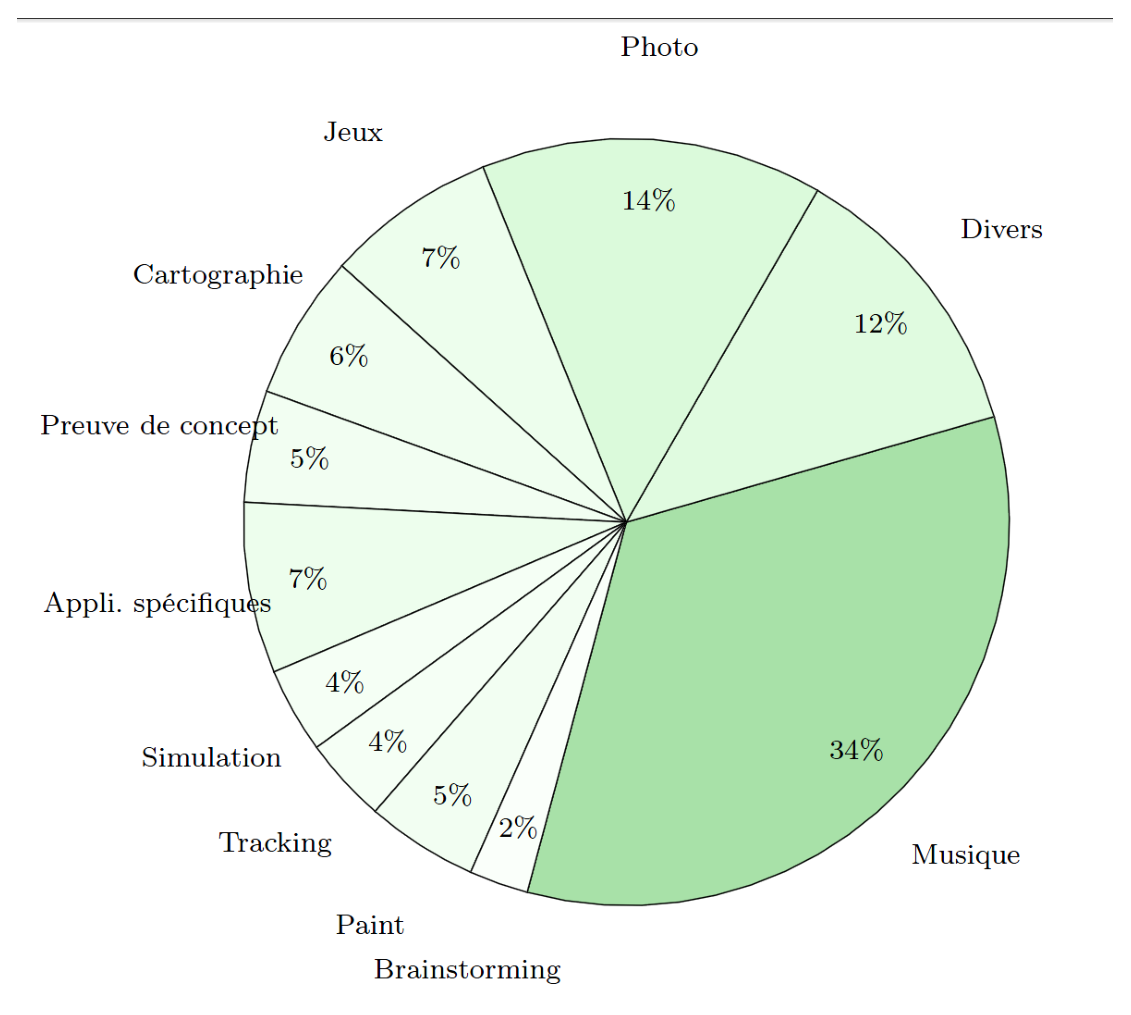
\includegraphics[scale=.9]{chap1/img-3}
\caption{R�partition des domaines d'utilisation des tables interactives en
2011}\label{fig:chap2:16}
\end{center}
\end{figure}

\subsection{Cas de l'application CBA}
\label{sec:chap2:2:1}
Consid\'{e}rons le cas d'\'{e}tude d'une application con\c{c}ue pour un desktop qui permet l'\'{e}laboration des bandes dessin\'{e}es (BD) telle que \textit{Comics Book Application }(CBA). Cette application est con\c{c}ue pour \^{e}tre utilis\'{e}e par un dessinateur de BD qui est assis devant son \'{e}cran en utilisant sa souris et son clavier. La fen\^{e}tre principale de l'application
CBA d\'{e}crite par la figure~\ref{fig:chap2:6} nous permet d'identifier trois zones majeures que sont la zone des menus correspondant aux composants graphiques situ\'{e}s en haut de la fen\^{e}tre principale, l'espace de travail qui contient les cadres d'une page de bande dessin\'{e}e et la zone de l\'{e}gende correspondant aux groupes, aux formulaires et listes \`{a} gauche de la fen\^{e}tre.

\begin{figure}[ht]
\begin{center}
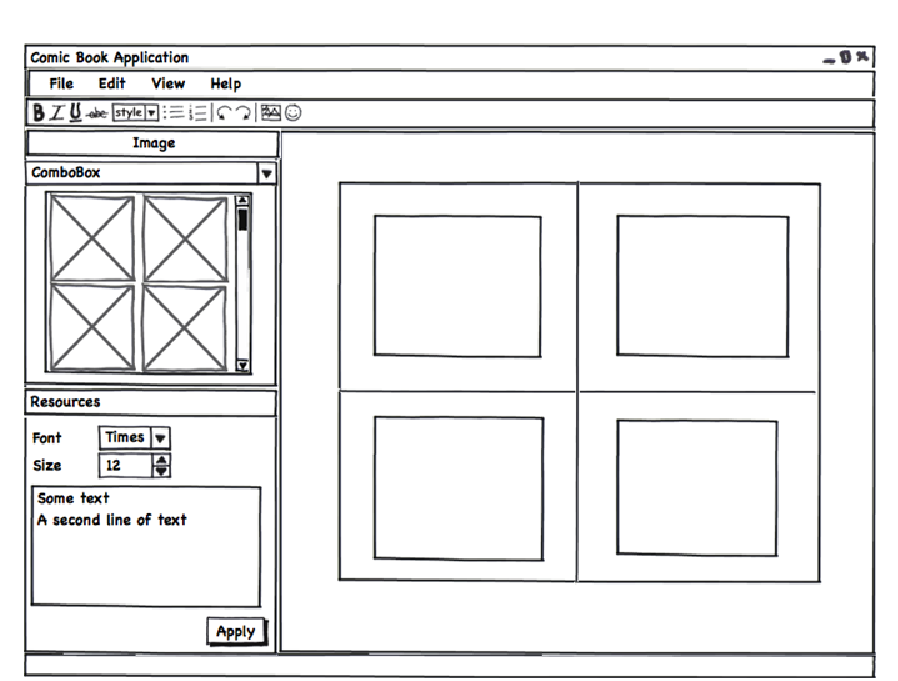
\includegraphics[width=413pt]{chap1/img-1}
\caption{Fen\^{e}tre principale de l'application CBA}
\label{fig:chap2:6}
\end{center}
\end{figure}


\subsection{Probl�matiques li�es � la migration des UI}
\label{sec:chap2:2:2}
La migration des UI des applications existantes vers une nouvelle plateforme tout en conservant le NF peut se faire en concevant une nouvelle UI pour la plateforme en se basant sur le NF et sur les sp�cificit�s de la plateforme d'arriv�e. Il est aussi possible de migrer une UI en l'adaptant � sa cible en tenant compte ou non des sp�cificit�s de cette cible. Ces deux types de migration d'UI (adaptation ou nouvelle conception) soul�vent plusieurs probl�mes.
\subsubsection{Probl�matiques li�es � une reconception de l'UI}
La reconception de l'UI suppose de s'appuyer sur le NF de l'application de d�part, particuli�rement sur les liens entre ce NF et l'UI � migrer et sur les sp�cificit�s de la plateforme d'arriv�e (les dispositifs d'interactions, les biblioth�ques graphiques, les crit�res ergonomiques, etc.). En effet, il est possible de d�duire une UI en se basant sur les liens entre le NF et l'UI, il existe des travaux qui pr�conisent la g�n�ration des UI � partir des descriptions des web services par exemple\cite{Kassoff2003}. 
La conception de l'UI en se basant sur le NF suppose de savoir comment d�duire une UI � partir d'une description abstraite du NF:
\begin{itemize}
	\item les composants graphiques qui composent l'UI, 
	\item la structure et le layout de ces composants graphiques, 
	\item le comportement de l'UI (c'est-�-dire l'enchainement des fen�tres et des activit�s de l'UI),
	\item et �valuer le respect des crit�res ergonomiques de l'UI g�n�r�e.
\end{itemize}

\subsubsection{Probl�matiques li�es � une adaptation de l'UI}
L'adaptation de l'UI pendant la migration suppose de s'appuyer sur les sp�cifications de l'UI � migrer d�crites par des mod�les abstraits et d'adapter ces mod�les � la plateforme d'arriv�e. Les mod�les servent � d�crire les diff�rents aspects de l'UI tels que les t�ches ou les activit�s d�crites par l'UI, le placement ou le layout des �l�ments de l'UI, les interactions entre l'utilisateur et l'UI, les styles de pr�sentations des aspects visuels (tailles et couleurs des textes, etc.) Le probl�me li� � la migration est: comment transformer les diff�rents aspects d'une UI pour qu'ils soient conforme aux sp�cificit�s de la plateforme cible? En effet la migration d'une UI desktop vers un smartphone peut entrainer le changement de layout et/ou du placement des �l�ments de l'UI de d�part. Et la diff�rence des moyens d'interactions entre un desktop et une table interactive implique une adaptation du mod�le d'interaction de l'UI de d�part par exemple.

\fbox{\parbox{0.9\textwidth}{
De mani�re g�n�rale, les migrations d'UI bas�es sur l'adaptation de l'existant �voquent des probl�mes li�es aux transformations des diff�rents aspects de l'UI pour la plateforme d'arriv�e.}}

 
\subsection{Probl�matiques li�es � la migration d'UI vers une table interactive}
\label{sec:chap2:2:3}
Dans le cas sp�cifique d'une migration d'UI vers une table interactive, les probl�matiques �voqu�es � la section~\ref{sec:chap2:2:2} peuvent �tre pr�cis�es d'avantages.  
En consid�rant l'application CBA (cf section~\ref{sec:chap2:2:1}), la migration de son UI sur une table interactive se fait en soulevant les questions suivantes:
\begin{itemize}
\item comment placer et organiser les �l�ments de l'UI de d�part pour une table interactive? \\
En effet, la fen�tre principale de l'application CBA est con�ue suivant la m�taphore de bureau  qui permet de d�crire les applications pour les ordinateurs personnels~\cite{AppleComputerInc1995}. Les menus sont plac�s en haut et � des positions fix�es, les outils ou les l�gendes sont toujours plac�s � gauche ou � droite et la zone de travail au centre. Cette structuration des zones permet aux utilisateurs des desktops de se retrouver  facilement quelque soit l'application.\\
Sur une table interactive, cette structuration n'est pas recommand�e car elle ne permet pas une utilisation par plusieurs utilisateurs et elle fixe l'orientation des composants graphiques de chaque zone. Pour l'application CBA, les diff�rentes zones de la structure de d�part peuvent �tre conserv�es mais chaque zone n'est plus associ�e � un espace g�ographique sp�cifique de l'�cran. Sur la droite de la figure~\ref{fig:chap2:18}, les diff�rentes zones de l'UI CBA de d�part n'ont plus de position fixe sur l'UI CBA de la table interactive � droite de la m�me figure.

\begin{figure}[h]
\begin{center}
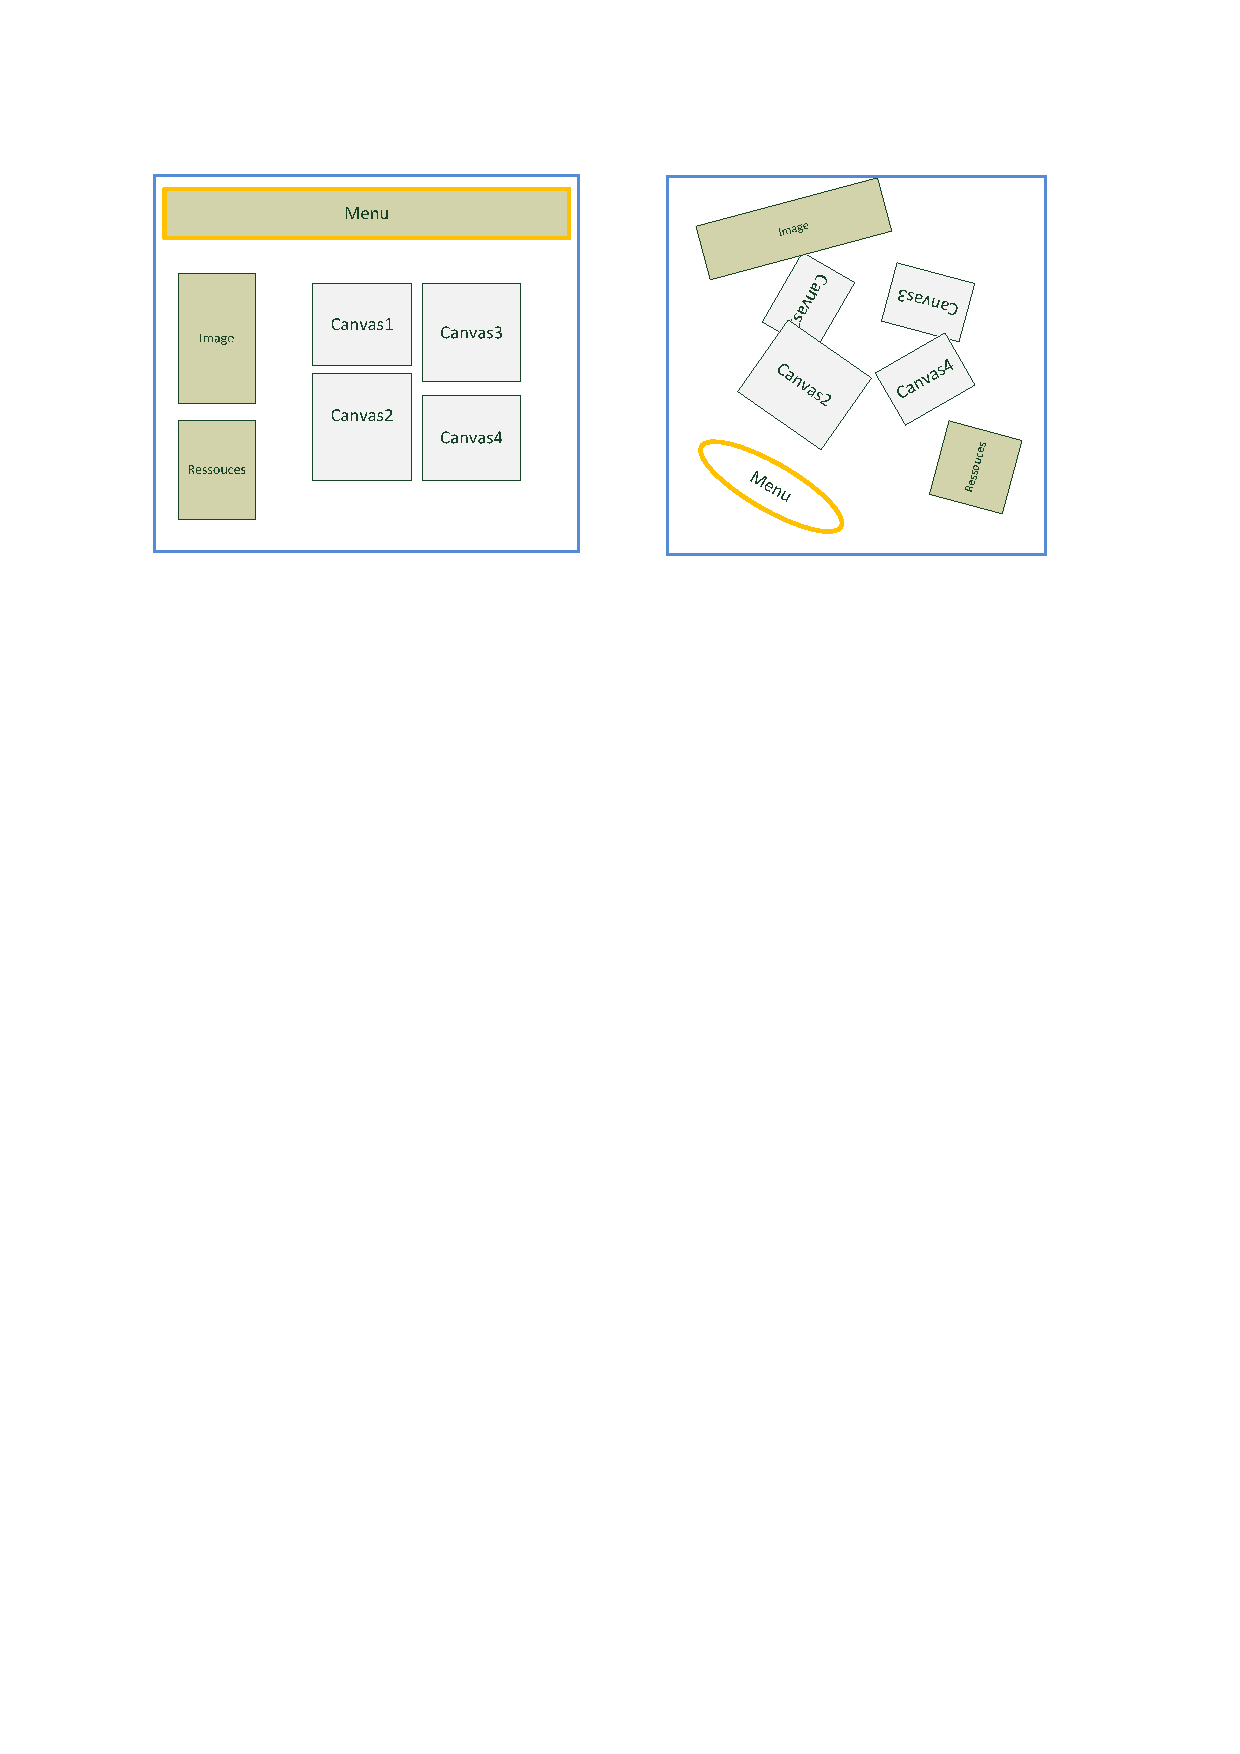
\includegraphics[width=432pt]{chap1/img-2}
\caption{Migration de la structure d'une UI Desktop sur une table interactive}\label{fig:chap2:18}
\end{center}
\end{figure}
\item comment utiliser les interactions (tactiles, tangiles) d'une table interactive avec l'UI de d�part?
\item comment prendre en compte la taille de la surface d'affichage d'une table interactive?
\item comment prendre en compte le nombre d'utilisateurs pendant la migration de l'UI de CBA? Cette probl�matique consiste aussi � transformer une UI mono utilisateur en UI collaborative dans le cas o� le nombre d'utilisateur est sup�rieur � un. Le projet CoWord ~\cite{Xia2004} permet � plusieurs utilisateurs d'utiliser le logiciel Microsoft Word en m�me temps mais pas sur un m�me support, en effet les utilisateurs sont dispers�s g�ographiquement et ils ont chacun un ordinateur de bureau. Dans notre cas les utilisateurs devront partager une m�me surface d'affichage qui est l'�cran de la table interactive cibl�e.
\end{itemize}
Dans la section suivante, nous d�taillerons ces probl�matiques en pr�sentant les sp�cificit�s des tables interactives � travers leur mod�le d'interaction et leurs principes de conception des UI.

\section{Sp�cificit�s de la migration d'UI vers les tables interactives}
\label{sec:chap2:3}
Les tables interactives sont des surfaces qui offrent la possibilit� d'interagir avec des syst�mes interactifs � travers des UI. Les sp�cificit�s d'interactions entre les utilisateurs et ces tables interactives peuvent �tre d�crites avec des interactions instrumentales~\cite{Beaudouin-Lafon2000}. Une interaction instrumentale est une action d'un utilisateur � l'aide de dispositifs physiques (�cran tactile par exemple) et de composants graphiques (boutons, scrolls par exemple) pour modifier ou acc�der � des objets d'un domaine (images, donn�es num�riques, etc.). Ensuite une interaction en sortie est une r�ponse traduite en une r�action ou un feedback par les instruments d'interaction en sortie. La figure~\ref{fig:chap2:1} montre les diff�rents �l�ments de ce mod�le d'interaction, les instruments servant de moyen d'interactions  pour l'utilisateur sont constitu�s de l'�cran tactile et des composants graphiques. La migration d'une UI d�crite suivant un autre mod�le d'interactions vers ce mod�le implique l'adaptation des objets du domaine et des interactions de l'UI de d�part aux nouveaux instruments qui constituent la plateforme d'arriv�e. L'adaptation des diff�rents aspects de l'UI de d�part � la table interactive, se fait suivant un ensemble de principes et des recommandations li�s aux tables interactives, dans l'objectif d'avoir une UI respectant ses crit�res ergonomiques.


Dans l'objectif d'identifier et de caract�riser les principes de conception des UI pour les tables interactives, cette section �tudie les diff�rents �l�ments qui composent le mod�le d'interaction d'une table interactive (instruments mat�riels, instruments logiciels, repr�sentation des interactions  en entr�e et en sortie entre les utilisateurs et les objets du domaine). Elle  pr�sente l'ensemble des principes de conception des UI li�es aux tables interactives n�cessaires pour la migration. 
	
\subsection{Mod�le d'interactions d'une table interactive}
Les instruments d'interactions constituent l'ensemble des dispositifs mat�riels et logiciels d'une table interactive qui permettent d'interagir avec un SI. Les dispositifs mat�riels d'interactions sont des moyens d'interactions en entr�e (actions) ou en sortie (r�actions et feedback) cf. figure~\ref{fig:chap2:1}. Et les biblioth�ques graphiques sont des instruments logiciels pour d�crire des interfaces utilisateurs graphiques dans le cadre des tables interactives. Dans ce paragraphe nous nous appuierons sur des tables interactives (Microsoft PixelSense, TangiSense, DiamondTouch, etc.) pour caract�riser les dispositifs mat�riels et d'interaction, les biblioth�ques graphiques et les modalit�s d'interactions des tables interactives. 

\begin{figure}[ht]
\begin{center}
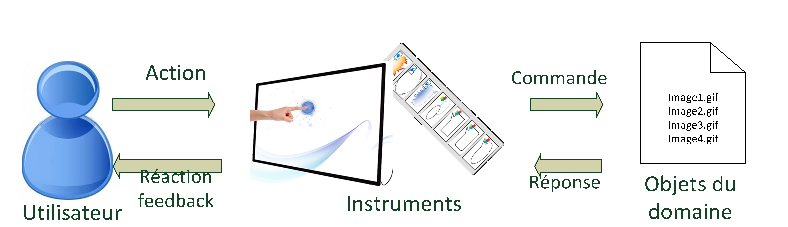
\includegraphics[width=360pt]{chap2/img-1}
\caption[b]{Mod�le d'interaction instrumentale d'une table interactive}
\label{fig:chap2:1}
\end{center}
\end{figure}
\subsubsection{Les dispositifs mat�riels d'interaction d'une table interactive}
\label{sec:chap2:3:1}
Dans ce paragraphe nous �tudions les instruments d'interactions de trois tables interactives. Nous �tudions d'abord DiamonTouch ~\cite{Dietz2001} qui est l'une des premi�re table interactive utilis�e dans un cadre non exp�rimental, elle fut industrialis�e par MERL~\cite{MitsubishiElectricResearchLaboratoriesb}, nous l'�tudions car elle comporte une biblioth�que graphique DiamondSpin et permet de d�crire des interactions multi utilisateurs, collaboratives et tactiles. Ensuite, l'on s'int�resse � metaDesk ~\cite{Ullmer1997} qui supporte que des objets tangibles comme moyen d'interaction. Enfin nous nous int�resserons aux tables Microsoft PixelSense 1.0 et 2.0 ~\cite{Microsoft2011} pour leurs biblioth�ques graphiques et leurs moyens d'interactions, contrairement aux deux autres tables pr�c�dentes, les tables Surface supportent � la fois les interactions collaboratives, tangibles et tactiles.

\paragraph {DiamondTouch}-
\label{sec:chap2:3:1:1}
Les moyens d'interaction de la table DiamonTouch sont une surface tactile non capacitif pour les interactions en entr�e et un vid�o projecteur pour les interactions en sortie. Cette table supporte des interactions multi utilisateurs et elle est capable d'identifier  les contacts de chaque utilisateus autour de la table. Elle ne supporte pas les interactions tangibles car elle ne peut pas d�tecter des objets ou des tags. Cette table permet de d�crire des UI collaboratives. Les UI collaboratives pour les tables interactives ont pour objectif de permettre � plusieurs utilisateurs de partager en m�me temps une UI.  Dans le cadre de la  table interactive DiamondTouch les utilisateurs d'une UI collaborative partagent un m�me espace (la table interactive) et il est possible de cr�er � chaque utilisateur son espace de travail. Cette solution implique une r�partition g�ographique fixe autour de la table. En effet pour migrer l'UI de l'application CBA par exemple sur une table DiamondTouch, il est indispensable de connaitre le nombre d'utilisateurs de l'UI migr�e car chaque utilisateur doit �tre assis sur une chaise pour utiliser la table(cf. figure~\ref{fig:chap2:17}). DiamondTouch ne permet aux utilisateurs d'�tre debout pendant l'utilisation de la surface d'affichage.  
 
\begin{figure}[h]
\begin{center}
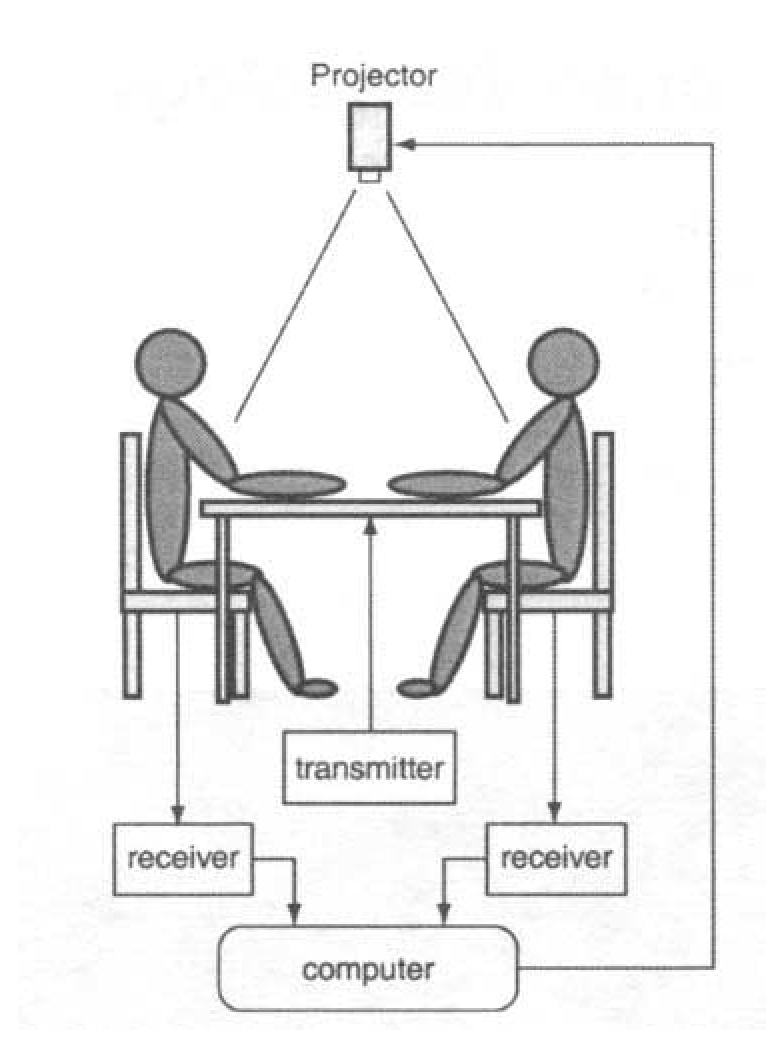
\includegraphics[scale=.4]{chap2/img-10}
\caption{Table interactive DiamondTouch}\label{fig:chap2:10}
\label{fig:chap2:17}
\end{center}
\end{figure}

\paragraph {metaDESK}-
\label{sec:chap2:3:1:2}
Les moyens d'interaction de la table metaDESK sont constitu�s des objets tangibles et de cam�ra infrarouge. Ces objets permettent � chaque utilisateur de manipuler des objets virtuels associ�s aux objets physiques. Elle ne limite pas le nombre d'utilisateurs comme la table DiamondTouch et permet � chaque utilisateur d'�tre mobile autour de la table. Cette Table permet de d�crire des UI tangibles (TUI).

Ulmer et Ishii ~\cite{Ishii1997} d�finissent un TUI comme des syst�mes interactifs qui utilisent des objets physiques pour repr�senter et utiliser des informations digitales. Le mapping entre le monde physique et digital peut se faire en repr�sentant les diff�rents composants graphiques d'une UI graphique � l'aide des objets concrets. La conception de TUI pour la table metaDESK~\cite{Ishii1997}, les concepteurs associent une lentille � une fen�tre, un plateau � un menu, etc. comme l'indique la figure~\ref{fig:chap2:12} d'instanciation physique des �l�ments GUI de metaDESK de la figure~\ref{fig:chap2:12}. Ce type d'association permet de concr�tiser des composants graphiques virtuels � travers des objets physiques.\\
Dans le cadre de la migration d'une UI desktop vers la table metaDESK, toutes les interactions de l'UI de d�part doivent �tre adapt�es ou �mul�es avec des objets tangibles. En consid�rant l'UI de l'application CBA par exemple, le formulaire \textit{Ressources} doit �tre affich� et rempli avec des objets tangibles, la s�lection de la taille ou de la police peuvent �tre �muler avec des objets circulaires en les tournant par exemple. Par ailleurs l'�mulation d'un clavier � l'aide d'un objet tangible pour la saisie des textes est possible mais n'est pas facilement utilisable~\cite{MenuTangible}. Les tables interactives uniquement tangibles comme metaDESK ou TangiSense~\cite{Kubicki2009} sont en g�n�rale con�ues pour faire de la r�alit� augment�e pour des applications de cartographie par exemple.
\begin{figure}[ht]
\begin{center}
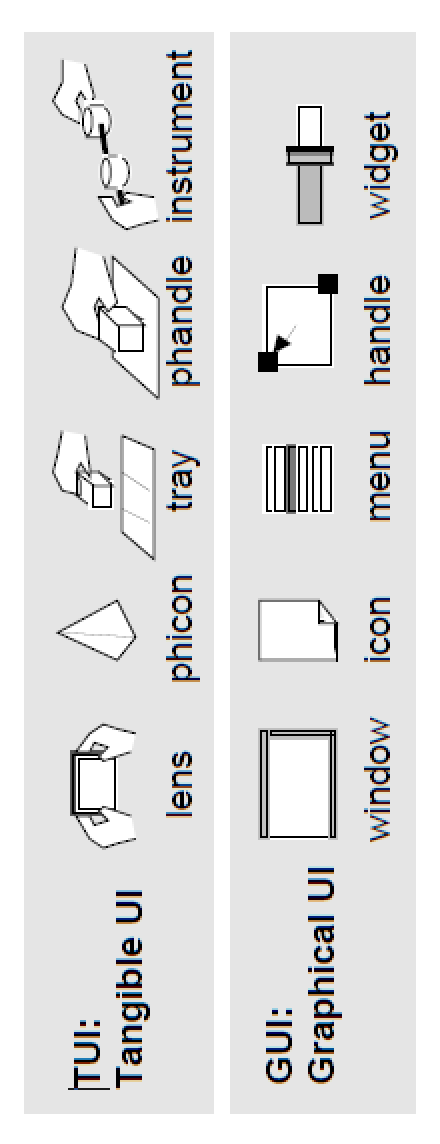
\includegraphics[angle=270,scale=.6]{chap2/img-12}
\caption{Instanciation physique des �l�ments GUI dans TUI}
\label{fig:chap2:12}
\end{center}
\end{figure}

\paragraph {Microsoft PixelSense }
\label{sec:chap2:3:1:3}
Les moyens d'interaction de la table interactive Microsoft PixelSense sont un �cran tactile permettant la reconnaissance des objets physiques, un clavier virtuel et des dispositifs sonores. Elles permettent de d�crire des UI tactiles et tangibles par l'utilisation des tags. Elles supportent  50 contacts simultan�s et permet donc de d�crire des UI multi utilisateurs dans la limite des contacts support�s. En effet une UI ne peut pas supporter plus de 50 points de contacts simultan�s, cette contrainte et la taille de l'�cran limite le nombre d'utilisateurs utilisant une application sur cette table au m�me moment.

Cette plateforme permet la description de TUI par la reconnaissance des Tags et la forme des objets. L'utilisation de tags permet de ne pas limiter les objets � utiliser dans la description des UI. Les tags sont des codes barres � deux dimensions qui sont facilement identifiables par la table surface. La Surface offre deux types tags : Identity tags et Byte tags\footnote{Les Identity tags sont des tags sur avec une plage de valeurs sur 128 bits, les Byte tags on une plage de valeurs sur 8 bits}. Ils peuvent �tre utilis�s pour reconna�tre des objets physiques ou les distinguer parmi plusieurs, pour d�clencher une commande ou une action (afficher un menu ou une application par exemple), pour pointer et orienter une application par un objet tagu� peut �tre utilis� pour le contr�le de volume car il peut d�tecter le changement d'angle d'un objet.

\paragraph{R�sum�}
\label{sec:chap2:3:1:4}
Les tables interactives de mani�re g�n�rale ont deux types de dispositifs physiques d'interactions: les dispositifs d'interaction en entr�e qui  peuvent �tre tactiles et/ou tangibles et les dispositifs d'interaction en sortie qui sont des surfaces d'affichage. Ces surfaces sont de tailles variables et de diff�rentes formes (rectangulaire, circulaire, etc.). Elles peuvent �tre dispos�es de mani�re horizontale (pour DiamondTouch, TangiSense, Microsoft PixelSense 1.0 et 2.0) ou de mani�re verticale (pour Microsoft PixelSense 2.0, etc. ).
 
Le nombre d'utilisateurs et leurs dispositions autour de la surface d'affichage sont des �l�ments qui permettent de caract�riser les interactions des tables interactives. En effet ces deux caract�ristiques impactent la conception des UI car une UI destin�e � plusieurs personnes doit permettre l'accessibilit� des diff�rentes fonctionnalit�s � tous les utilisateurs et elle doit aussi prendre en compte le partage des �l�ments de l'UI (menus, visualisation des contenus, etc.)

\fbox{\parbox{0.9\textwidth}{
Les dispositifs mat�riels des tables interactives permettent de d�crire des UI multi utilisateurs, co-localis�es, tactiles et tangibles. La migration des UI des applications qui ne prennent pas en compte ces caract�ristiques soul�ve des probl�matiques li�es � la prise en compte des diff�rents moyens d'interactions en entr�e et en sortie des tables interactives, du nombre d'utilisateurs et de la disposition des utilisateurs par rapport � la surface d'affichage.}}

\subsubsection{Biblioth�ques graphiques des tables interactives}
\label{sec:chap2:3:2}
Les biblioth�ques graphiques sont des bo�tes � outils logiciels qui contiennent des �l�ments pour d�crire des UI graphiques; dans le mod�le d'interactions des tables interactives, les composants graphiques sont des instruments logiciels qui permettent de faire le lien entre les dispositifs mat�riels d'interactions et les objets d'un domaine. Elles offrent des composants graphiques adapt�s aux moyens d'interactions d'une plateforme sp�cifique. Dans cette section nous pr�sentons quelques biblioth�ques graphiques sp�cifiques aux tables interactives.

\paragraph{DiamondSpin}
\label{sec:chap2:2:2:1} ~\cite{Shen2004} est une biblioth�que graphique pour table interactive qui offre des composants graphiques adapt�s � plusieurs utilisateurs. En effet, elle offre des composants graphiques qui permettent : une manipulation des documents visuels, la manipulation directe des �l�ments d'UI, la possibilit� d'utiliser ses doigts, un stylet ou un clavier comme moyen d'interaction, la rotation des composants graphiques, et la possibilit� de cr�er et de g�rer des espaces priv�s pour chaque utilisateur. Les composants graphiques \textit{DSContainer, DSPanel, DSWindow, DSFrame} (cf. figure \ref{fig:chap2:2}) par exemple permettent d'avoir un container qui regroupe un ensemble de composants graphiques qu'un utilisateur peut d�placer en fonction de sa position. 
\begin{figure}[ht]
\begin{center}
\includegraphics[angle=90, width=258pt]{chap2/img-16}
\caption{Instances des container DiamondSpin}\label{fig:chap2:2}
\end{center}
\end{figure}

\paragraph{Surface SDK  1.0 et 2.0}\label{sec:chap2:2:2:2} ~\cite{Microsoft2012} sont des API et des bo�te � outils pour d�velopper des applications pour une Table interactive Microsoft (1.0 et 2.0). Ils font partie du Framework .Net et offrent des biblioth�ques graphiques pour concevoir des UI WPF ~\cite{MicrosoftWPF2012} et XNA ~\cite{MicrosoftXNA2012}. Ces biblioth�ques graphiques offrent des composants graphiques permettant la reconnaissance des formes d'objets, l'utilisation des tags, 50 points de contacts simultan�s, la d�tection de l'orientation des touches, etc. Ces facilit�s par rapport � la biblioth�que graphique DiamondSpin �vitent au programmeur la gestion du d�placement ou la rotation des composants graphiques par exemple. En effet un \textit{ScatterView} (Figure \ref{fig:chap2:3}) d�finie le d�placement ou la rotation de mani�re intrins�que.
\begin{figure}[ht]
\begin{center}

\includegraphics[width=200pt]{chap2/img-4}
\caption{Exemple de ScatterView}
\label{fig:chap2:3}
\end{center}
\end{figure}
\paragraph{R�sum�}
\label{sec:chap2:2:2:3}
La biblioth�que DiamondSpin permet d'utiliser la table DiamondTouch � l'instar d'un bureau virtuel par plusieurs personnes assises autour de la table. Elle offre aussi des composants graphiques bas�s sur la m�taphore du papier~\cite{Besacier2007}. La m�taphore du papier permet l'utilisation des �l�ments graphiques d'un container comme une feuille de papier en ayant la possibilit� de plier, retourner, dupliquer ou d�chirer le container, sur une table interactive cette m�taphore permet de conserver les actions qu'on r�alise sur une table de travail concr�te.\\ 
La biblioth�que Surface SDK permet de d�crire des TUI � l'aide des tags. De mani�re g�n�rale, les biblioth�ques graphiques des tables interactives offrent des composants graphiques qui ont des interactions (rotation, redimensionnement, d�placement, tags, etc.) adapt�es pour la description des UI pour les tables interactives. Elles permettent d'affiner les caract�ristiques des tables interactives en pr�cisant si une table interactive supporte ou non des interactions tangibles, si elle a des composants graphiques accessibles par tous les utilisateurs par exemple.\\

\fbox{\parbox{0.9\textwidth}{
Dans le cadre de la migration, le changement de biblioth�que graphique implique une nouvelle conception de l'UI de d�part pour rendre accessible ses fonctionnalit�s sur la plateforme d'arriv�e en utilisant les composants graphiques adapt�s aux dispositifs physiques de la table interactive.}}

\subsubsection{Modalit�s d'interactions}
\label{sec:chap2:3:3}
Nigay ~\cite{Nigay1994a} propose une d�finition de la modalit� d'interaction comme un couple <d, l> constitu�  d'un dispositif d'interaction et d'un langage d'interaction ~\cite{Nigay1994a}: - d d�signe un dispositif physique (par exemple, une souris, une cam�ra, un �cran, un haut-parleur), - l d�note un syst�me repr�sentationnel, c'est-�-dire un syst�me conventionnel structur� de signes assurant une fonction de communication (par exemple, un langage pseudo naturel, un graphe, une table).

\fbox{\parbox{0.9\textwidth}{
La migration des UI vers les tables interactives implique un changement des dispositifs d'interactions et la possibilit� de d�crire des �quivalences entre les modalit�s d'interactions des plateformes de d�part et celles des tables interactives.}}\\

Dans cette section nous abordons la probl�matique li�e aux changements des modalit�s d'interactions des UI � migrer. En effet comment d�crire les interactions de l'UI de d�part � l'aide des modalit�s d'interactions de la plateforme d'arriv�e? Pour r�pondre � cette question nous �tudions au paragraphe \ref{sec:chap2:3:1} les probl�mes li�es aux changements de modalit�s d'interactions pendant la migration. Et au paragraphe \ref{sec:chap2:3:2} nous pr�sentons quelques mod�les d'interactions abstraite qui permet de d�crire les interactions ind�pendamment des modalit�s d'interactions.

\paragraph{Changement de modalit� d'interaction}-
\label{sec:chap2:2:3:1}
Consid�rons comme plateforme de d�part un desktop compos� d'un �cran comme moyen d'interaction en sortie et d'un clavier et d'une souris comme moyen d'interaction en entr�e. 
\begin{itemize}
\item La modalit� d'interaction en sortie M1  du  desktop est d�crite par l'�cran et par le langage de description des UI 2D (L1), M1=<Ecran, L1>. Le langage L1 correspond aux composants graphiques tels que labels, champ de texte, bo�te de dialogue, etc. d'une biblioth�que graphique.
\item La modalit� d'interaction en entr�e M2  du  desktop est d�crite par le clavier et par le langage des commandes (L2), M2=<Clavier, L2>. Le langage L2 d�crit pour chaque actions les t�ches r�alisables � l'aide d'un clavier sur une UI graphique, ces actions sont par exemple : copier avec Ctrl+C, couper avec Ctrl+X, coller avec Ctrl+V, saisir un texte avec les touches alphanum�riques, valider avec la touche entr�e, etc. 
\item La modalit� d'interaction en entr�e M3  du  desktop est d�crite par la souris et par le langage de manipulation directe d'une UI 2D (L3), M3=<Souris, L3>. Le langage L3 d�crit les actions r�alisables � l'aide d'une souris sur une UI graphique, ces actions sont par exemple : cliquer et valider pour s�lectionner un composant graphique, cliquer et d�placer pour s�lectionner un texte, d�placer un �l�ment, redimensionner, etc. 
\end{itemize}

Et consid�rant maintenant que la table interactive cible est compos�e d'un �cran tactile, d'un clavier virtuel et de la reconnaissance des objets physiques comme moyens d'interactions.
\begin{itemize}
\item La modalit� d'interaction en sortie M'1  de la table interactive est d�crite par l'�cran tactile et par le langage de description des UI 2D (L'1), M'1=<Ecran Tactile, L'1>. Le langage L'1 correspond � la biblioth�que graphique de la table interactive qui contient les composants graphiques tels que labels, champ de texte, images, fen�tre, etc.
\item La modalit� d'interaction en entr�e M'2  de la table interactive est d�crite par l'�cran tactile et par le langage de manipulation tactile d'une UI 2D (L'2), M'2=< Ecran Tactile, L'2>. Le langage L'2 d�crit les actions utilisateurs sur un �cran tactile. Ces actions sont par exemple : toucher avec un doigt pour activer ou s�lectionner un �l�ment, toucher avec deux doigts et d�placer pour agrandir, r�duire, tourner des composants graphiques, etc.
\item La modalit� d'interaction en entr�e M'3  de la table interactive est d�crite par le clavier virtuel  et par le langage de commande  (L'3), M'3=< Ecran Tactile, L'3>. Le langage L'3 d�crit les actions utilisateurs r�alisables avec un clavier virtuel tel que saisir un texte.
\item La modalit� d'interaction en entr�e M'4  de la table interactive est d�crite par l'�cran tactile et par le langage de manipulation des objets tangibles (L'4), M'4=< Objets Tangibles, L'4>. Le langage L'4 d�crit les actions utilisateurs sur un �cran tactile � l'aide des objets tangibles. Ces actions sont par exemple : poser un objet pour afficher un menu ou un formulaire, d�placer un objet physique pour d�placer l'objet virtuel associ�, tourner un objet physique pour s�lectionner une fonctionnalit�, etc.
\end{itemize}

Les langages d'interaction L1 et L'1 permettent de d�crire les interactions en sortie des UI des applications source et cible. Ces langages peuvent �tre mod�lis�s en se basant sur des bo�tes � outils ind�pendantes des dispositifs d'interactions en sortie. Crease dans ~\cite{December2001} propose une bo�te � outils d�crivant des widgets multimodales et ind�pendantes des dispositifs d'interactions en sortie. Les widgets de Crease~\cite{December2001} restent cependant li�es aux dispositifs d'interactions en entr�e tels que le clavier et la souris.

Les langages d'interaction L2, L3, L'2, L'3 et L'4 quant � eux permettent de d�crire et d'interpr�ter les interactions en entr�e des utilisateurs des plateformes de d�part et d'arriv�es. Ces langages d'interaction permettent d'associer � chaque action de l'utilisateur un comportement ayant un sens dans l'UI de l'application. Les actions utilisateurs telles que cliquer, s�lectionner, Ctrl+C, poser un objet, etc. d�pendent des dispositifs d'interactions tandis que les comportements de l'UI d�pendent du type d'UI et de l'interpr�tation souhait�e par le concepteur.\\

\paragraph{�quivalences des modalit�s d'interactions}
La migration de la plateforme desktop vers une table interactive peut �tre consid�r�e comme un processus de changement de modalit�s d'interactions. En effet dans le but de r�utiliser l'UI d'une application de d�part avec les dispositifs d'interactions de la plateforme d'arriv�e, il est possible d'�tablir des �quivalences entre les dispositifs d'interaction et les langages d'interactions des plateformes de d�part et d'arriv�e.\\
Pour d�crire les interactions d'une UI de d�part � l'aide des dispositifs d'interaction d'une table interactive, l'une des approches � envisager peut �tre la mise en correspondance des dispositifs d'interactions en �tablissant des �quivalences entre les diff�rentes modalit�s d'interactions des plateformes source et cible. Ce qui consiste par exemple � d�crire des �quivalences d'abord entre les modalit�s d'interactions en sortie  M1 et M'1 et ensuite entre les modalit�s d'interactions en entr�e M2, M3 et M'2, M'3 M'4.\\
L'�quivalence entre M1 et M'1 consiste � comparer les deux dispositifs qui sont des �crans qui peuvent afficher des UI graphiques et les langages L1 et L'1 qui ont des composants graphiques appartenant � des biblioth�ques graphiques diff�rentes.
L'�quivalence entre les modalit�s d'interactions en entr�e n'est possible que si l'on peut comparer les langages L2, L3, L'2, L'3 et L'4. Ces langages sont d�crits en fonction des dispositifs d'interaction et aussi en fonction des applications, en effet chaque concepteur peut d�crire un langage propre � son application, l'objectif de ces langages �tant de faciliter l'interaction entre un dispositif physique (clavier, souris, �cran tactile, etc.) et l'UI de l'application.


%\paragraph{R�sum�}
%\label{sec:chap2:2:3:3}
%Dans le processus de migration vers une table interactive, le paragraphe~\ref{sec:chap2:2:3:1} indique les diff�rences entre les modalit�s d'interactions en entr�e sont importantes au niveau du nombre de dispositifs physiques et des langages. 


\subsection{Propri�t�s caract�ristiques du mod�le d'interactions des tables interactives }
\label{sec:chap2:3:4}
Les �l�ments du mod�le d'interactions instrumentales des tables interactives tels que les dispositifs mat�riels d'interactions en entr�e et en sortie, les biblioth�ques graphiques ou les modalit�s d'interactions nous permettent d'identifier des propri�t�s caract�ristiques des tables interactives qui impactent la conception des UI pour des tables interactives. 
\subsubsection{Dispositifs d'interactions en entr�e }
\label{sec:chap2:3:4:1}
Ces dispositifs influencent la conception des interactions. Dans le cadre des tables interactives nous identifions deux propri�t�s qui correspondent aux moyens d'interactions tangibles et tactiles.

\fbox{\parbox{0.9\textwidth}{
\begin{prop}{Tangibilit� des interactions}\label{prop:chap2:1}\end{prop}
Les dispositifs d'interactions en entr�e permettent d'associer des objets physiques aux fonctionnalit�s\footnote{les objets physiques peuvent �tre utilis�s pour activer des fonctionnalit�s} ou aux composants graphiques\footnote{les objets physiques peuvent aussi �tre utilis�s pour afficher ou d�placer des objets virtuels} d'une UI.
}}

\fbox{\parbox{0.9\textwidth}{
\begin{prop}{Tactibilit� des interactions}\label{prop:chap2:2}\end{prop}
Les dispositifs d'interactions en entr�e des tables interactives permettent de d�crire des manipulations directes des UI telles que la s�lection, l'�dition, le redimensionnement, le d�placement, etc. }}

\subsubsection{Dispositifs d'interactions en sortie }
\label{sec:chap2:3:4:2}
Ce sont les surfaces d'affichage des tables interactives, les propri�t�s caract�ristiques li�es � la taille et � la disposition des tables interactives qui impactent la conception des UI.\\

\fbox{\parbox{0.9\textwidth}{
\begin{prop}{Taille de la surface d'affichage}\label{prop:chap2:3}\end{prop}
Cette propri�t� permet d'adapter la taille des composants graphiques par rapport � la taille de l'�cran pour faciliter l'utilisation de l'UI.
}}\\

\fbox{\parbox{0.9\textwidth}{
	\begin{prop}{Disposition de la surface d'affichage}\label{prop:chap2:4}\end{prop}
	La surface d'affichage peut �tre dispos�e de mani�re horizontale comme une table de travail ou de mani�re verticale comme un tableau collaboratif. Ces dispositions influencent l'orientation et l'utilisation des composants graphiques d'une UI.
}}
\subsubsection{Utilisateurs des tables interactives }
\label{sec:chap2:3:4:3}
Les utilisateurs influencent la conception de l'UI par leur nombre et leur r�partition autour de la surface d'affichage.\\

\fbox{\parbox{0.9\textwidth}{
	\begin{prop}{Nombre d'utilisateurs}\label{prop:chap2:5}\end{prop}
	Cette propri�t� permet de savoir comment disposer les �l�ments de l'UI pour faciliter l'accessibilit� en fonction du nombre d'utilisateurs.
}}
\\

\fbox{\parbox{0.9\textwidth}{
	\begin{prop}{R�partition des utilisateurs }\label{prop:chap2:6}\end{prop}
	Cette propri�t� permet de savoir comment d�crire la collaboration entre les utilisateurs autour de la table.
	La r�partition de l'espace de travail de chaque utilisateur peut se faire par une division g�ographique de la surface ou permettre aux utilisateurs d'acc�der � toute la surface. 
}}
\subsection{Principes de conception d'UI pour les tables interactives}
\label{sec:chap2:3:5}
Le paragraphe \ref{sec:chap2:3:3} nous montre les diff�rences de modalit�s d'interactions entre un desktop et une table interactive. Ces diff�rences impactent aussi la conception d'UI pour ces deux plateformes. Besacier et \textit{al.} montrent que la r�utilisation des applications desktop sur les tables interactives en adaptant les �l�ments de l'UI aux m�taphores du papier par exemple facilite l'utilisation des UI ~\cite{Besacier2007}. Par ailleurs, une r�utilisation d'une application desktop sur des tables interactives sans prise en compte de ses sp�cificit�s pose deux probl�matiques majeures: la transformation de l'UI de d�part en UI collaborative d'une part et la transformation d'une GUI en TUI d'autre part. Ces deux caract�ristiques font parties de l'ensemble des principes qui guident la conception des UI pour les tables interactives.\\

\fbox{\parbox{0.9\textwidth}{ Les principes de conception d'UI pour une plateforme constituent un ensemble de recommandations pour les concepteurs d'UI qui indiquent comment d�crire les aspects tels que les interactions instrumentales, le layout (ou le placement des �l�ments graphiques), les activit�s d'une UI et aussi les styles de pr�sentations (couleurs, polices, tailles, etc).}}

Les principes de conceptions sont des recommandations de haut niveau qui doivent �tre traduites en r�gles formelles utilisables pendant la migration~\cite{Vanderdonckt1997}.

Dans cette section nous caract�risons les principes de conception pour la migration des UI vers les tables interactives en trois cat�gories: les principes de conception pour les UI tangibles, les principes de conception pour les UI collaboratives et colocalis�es et enfin les autres principes de conception d'UI sur une grande surface d'affichage telles que la taille et la position de la surface d'affichage, l'utilisation en 360 degr� de l'UI et le style de l'UI.

\subsubsection{Corpus des principes de conception d'UI pour Microsoft PixelSense}
\label{sec:chap2:3:5:1}
Les principes de conception d'UI pour une Microsoft PixelSense sont d�crits sous forme de guidelines (ou recommandations) dans le document \textit{User Experience Design Guideline}~\cite{Microsoft2011}. Ces guidelines sont le fruit des exp�riences des utilisateurs ayant d�velopp� des UI pour cette plateforme. L'objectif de ces guidelines est de faciliter la conception des interfaces utilisateurs naturelles~\cite{Steinberg2012} et intuitives. Ces guidelines couvrent plusieurs aspects du processus de conception des UI tels que la conception des interactions entre les UI et les utilisateurs finaux, les guides de styles pour une coh�rence visuelle, les guides d'utilisation des textes, etc. 

\subsubsection{Guidelines pour TUI}
\label{sec:chap2:3:5:2}
Cette cat�gorie regroupe les recommandations qui permettent de d�crire le comportement des �l�ments de l'UI qui sont des objets virtuels d'une part et l'association entre ces objets virtuels et les objets tangibles d'autre part. L'association peut se faire par des tags qui permettent de marquer les objets physiques ou en se basant sur la forme des objets physiques. Les guidelines de cette cat�gorie sont inspir�es par la propri�t�~\ref{prop:chap2:1} de tangibilit� des interactions.


\shadowbox{\parbox{0.8\textwidth}{
\begin{guide}\label{guide:1}Comportement des objets virtuels\end{guide}
Les comportements des �l�ments d'une TUI pendant leurs utilisations doivent correspondre aux objets physiques. Les �l�ments (ou objets virtuels) de l'UI  � migrer doivent �tre associ�s � des objets physiques dans le but d'afficher des  menus, des formulaires ou des fen�tres et aussi dans le but d'activer ou d'utiliser des fonctionnalit�s. 
}}
%\\


\shadowbox{\parbox{0.8\textwidth}{
\begin{guide}\label{guide:2}Objets physiques tagu�s\end{guide} 
Un tag est associ� � un objet virtuel d'une TUI (les objets virtuels sont identifi�s gr�ce � la guideline~\ref{guide:1}). Le d�placement, l'orientation et la position du tag sur l'�cran peuvent �tre associ�s � des interactions en entr�e ou � des comportements de l'objet virtuel associ�. 
}}\\


\shadowbox{\parbox{0.8\textwidth}{
\begin{guide}\label{guide:3}Forme des objets physiques\end{guide}
La forme d'un objet physique peut �tre associ� � un objet virtuel ou � une fonctionnalit�. Le d�placement, l'orientation et la position d'un objet physique sur l'�cran peuvent �tre associ�s � des interactions en entr�e ou � des comportements de l'objet virtuel associ�. L'utilisation de la forme des objets physiques comme moyen d'interaction en entr�e n�cessite un module de reconnaissance de la forme d'un objet tangible. 
}}\\

En consid�rant l'UI de l'application CBA � la figure~\ref{fig:chap2:6}, le menu principal et le formulaire \textit{Ressources} par exemple peuvent �tre associ�s � un objet physique pour les afficher facilement sur l'�cran. Les r�gles formelles issues de la guideline~\ref{guide:1} permettront d'identifier et de transformer les �l�ments concrets de l'UI \\ Les tags permettent par exemple d'utiliser deux objets de la forme avec des couleurs diff�rentes et marqu�s  des deux diff�rents tags pour afficher un menu ou un formulaire. 

\subsubsection{Guidelines pour UI collaborative}
\label{sec:chap2:3:5:3}
Cette cat�gorie regroupe les recommandations pour la conception d'une UI collaborative et colocalis�e pour une table interactive. Les guidelines sont li�es � la propri�t�~\ref{prop:chap2:5} caract�risant le nombre d'utilisateurs et � la propri�t�~\ref{prop:chap2:6} qui caract�rise leur r�partition autour de la surface d'affichage. Elles sont aussi li�es � la propri�t�~\ref{prop:chap2:3} et � la propri�t�~\ref{prop:chap2:4} qui caract�rise la taille et la disposition (horizontale ou verticale) de la surface d'affichage des tables interactives. 

\shadowbox{\parbox{0.8\textwidth}{
\begin{guide}\label{guide:4}Nombre d'utilisateurs de l'UI migr�e\end{guide}
Cette guideline pr�conise de prendre en compte le nombre d'utilisateurs de l'UI apr�s la migration. Les UI d'une table interactive peuvent �tre collaboratives (plusieurs utilisateurs) ou non (dans le cas d'un seul utilisateur). Elle impacte  le couplage entre les t�ches et les utilisateurs (qui est sp�cifi� par la guideline~\ref{guide:5}), l'organisation de la surface de travail (qui est sp�cifi�e par la  guideline~\ref{guide:6}) et l'accessibilit� des �l�ments d'une UI collaborative (qui est sp�cifi�e par la guideline~\ref{guide:7}).}}


\shadowbox{\parbox{0.8\textwidth}{
\begin{guide}\label{guide:5}Couplage t�ches et utilisateurs d'une UI\end{guide}
Elle est une sp�cification de la guideline~\ref{guide:4}, car elle pr�conise dans le cas d'une UI multi utilisateurs :
\begin{itemize}
 \item d'�liminer toute les bo�tes de dialogues bloquantes pour les autres utilisateurs de l'UI.
 \item de dupliquer certains �l�ments de l'UI pour permettre � tous les utilisateurs d'acc�der aux �l�ments de l'UI.
\end{itemize}}}


\shadowbox{\parbox{0.8\textwidth}{
\begin{guide}\label{guide:6}Partage de l'espace de travail\end{guide}
Cette guideline sp�cifie la guideline~\ref{guide:4} en pr�conisant des composants graphiques qui facilitent le partage de l'�cran dans le cas d'une UI multi utilisateurs.
L'espace de travail doit:
\begin{itemize}
\item permettre � une personne d'utiliser une UI sans avoir l'aide d'autres utilisateurs,
\item permettre � un utilisateur d'utiliser l'UI sans interrompre les utilisateurs pr�sents.
\end{itemize}
 }}
 
 
Le partage de l'espace de travail est impl�ment� de diverses mani�res en fonction des tables interactives. La table DiamondTouch~\cite{Dietz2001} par exemple permet aux concepteurs d'associer un utilisateur � une zone de l'�cran. Cependant la table Microsoft PixelSense quant � elle ne permet pas une division de l'�cran en zones associ�es aux utilisateurs ou � des fonctionnalit�s. La figure~\ref{fig:chap2:14} illustre une division de l'�cran en quatre zones, ce type de partage d'�cran n'est pas autoris� par les guidelines de la table Surface. Dans le cadre de la migration d'UI vers les tables interactives, nous pensons que la division de l'�cran en plusieurs zones ne permet pas de d�crire des UI collaboratives si elle ne permet pas d'�changes entre les utilisateurs et leur mobilit� autour de l'�cran.
\begin{figure}[h]
\begin{center}
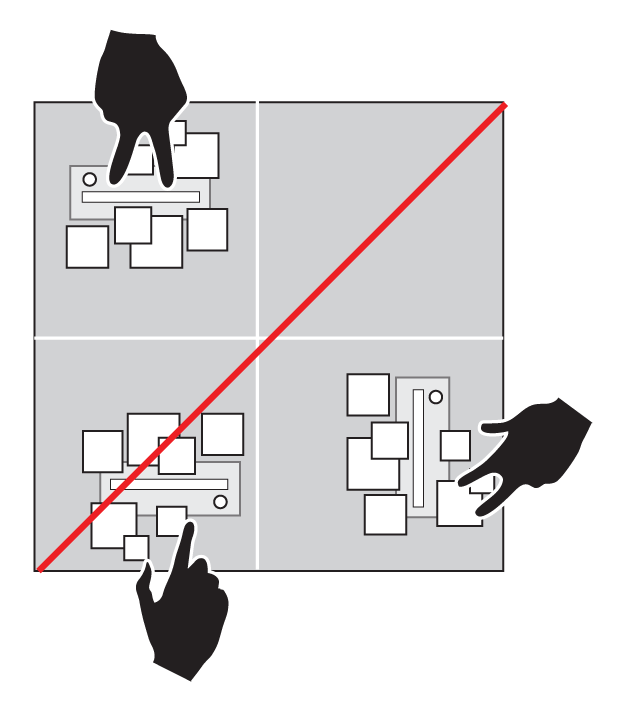
\includegraphics[angle=270,scale=.2]{chap2/img-22} 
\caption{Illustration de partage d'espace entre plusieurs utilisateurs}
\label{fig:chap2:14}
\end{center}
\end{figure}


\shadowbox{\parbox{0.8\textwidth}{
\begin{guide}\label{guide:7}Utilisation 360 degr� de l'UI\end{guide}
Cette guideline permet de sp�cifier la guideline~\ref{guide:4} car elle pr�conise la s�lection des composants graphiques pouvant �tre utilis�s partout autour de la table. Elle rend accessible les �l�ments d'une UI migr�e et renforce la collaboration entre les utilisateurs.}}
\\


La figure \ref{fig:chap2:13} illustre � un cas d'utilisation des composants graphiques utilisables � 360�. 
\begin{figure}[h]
\begin{center}
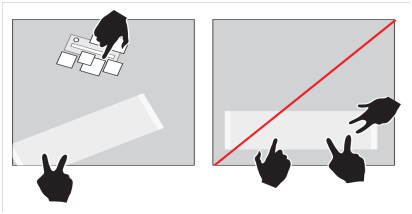
\includegraphics[angle=270,scale=.4]{chap2/img-13} 
\caption{Illustration de la propri�t� 360�}
\label{fig:chap2:13}
\end{center}
\end{figure}

En consid�rant que l'UI de l'application CBA (cf. figure~\ref{fig:chap2:6}) est migr�e vers une table Surface pour quatre dessinateurs de BD par exemple. Les ressources (images, ballons, etc.) utilis�s pour la conception des BD doivent �tre accessibles par les quatre utilisateurs. La guideline~\ref{guide:6} pr�conisant le partage de l'espace de travail et la guideline~\ref{guide:6} pr�conisant l'utilisation des objets 360 degr� permettent de d�crire une UI sans layout avec des groupes d'�l�ments utilisables � 360�. La guideline~\ref{guide:5} par exemple permettra de supprimer les composants graphiques bloquants tels que les boites de dialogues de l'UI de l'application CBA.

\subsubsection{Autres guidelines pour les UI sur surface}
\label{sec:chap2:3:5:4}
Les deux cat�gories de guidelines pr�sent�es ci-dessus qui permettent de d�crire des UI tangibles et des UI collaboratives (cf. section~\ref{sec:chap2:3:5:3}) ne constituent pas le corpus des guidelines applicables pendant la migration d'une UI vers une table interactive. En effet les apects de l'UI li�s au style des composants graphiques, des textes  de l'UI et les aspects li�s aux interactions tactiles ne sont pas pris en compte par ces deux cat�gories de guidelines. 
Cette troisi�me cat�gorie regroupe les guidelines de mise en {\oe}uvre des interactions tactiles et des styles de l'UI.
\paragraph{Guidelines pour les interactions tactiles}-
Les tables interactives permettent en g�n�ral de d�crire des interactions tactiles. L'ensemble des actions tactiles de l'utilisateur sont interpr�t�es par le dispositif d'interaction en entr�e. Dans le cadre des UI tactiles, il existe des actions tactiles standards pour des interactions de redimensionnement, de d�placement ou de rotation. Par exemple les guidelines des interactions tactiles pour une table Surface~\cite{Microsoft2011} identifient l'ensemble des gestes recommand�s aux concepteurs pour la s�lection, l'activation, le d�placement, la rotation, le zoom, etc. Cette cat�gorie de guidelines est li�e � la propri�t�~\ref{prop:chap2:2} de tactibilit� des interactions d'une table interactive.

\fbox{\parbox{0.9\textwidth}{
Dans le cadre de la migration de l'UI de l'application CBA  vers les tables interactives Surface, il est indispensable de pouvoir d�crire des correspondances entre les interactions tactiles et les interactions du clavier et de la souris de l'UI d�part.
}}

\paragraph{Guidelines pour le styles } - 
Cette sous cat�gorie regroupe l'ensemble des recommandations pour la personnalisation des aspects visuels d'une UI pour une table interactive. 
Ces guidelines peuvent �tre utilis�es dans le cadre d'une migration faisant intervenir les concepteurs comme des exemples pour les inspirer du choix de la forme, des couleurs, des icons et aussi de la diposition des textes d'une UI.
Dans le cas du sc�nario de migration, le formulaire \textit{Ressources} par exemple peut �tre migr� suivant comme l'indique le tableau~\ref{tab:chap2:1}. 

\begin{table}[h]
\begin{center}
\vspace{3pt} \noindent
\begin{tabular}{|p{143pt}|p{271pt}|}
\hline
Formulaire de l'application de d\'{e}part& Formulaire migr� en prenant en compte les guidelines de styles\\ 
\hline
\parbox{143pt}{ 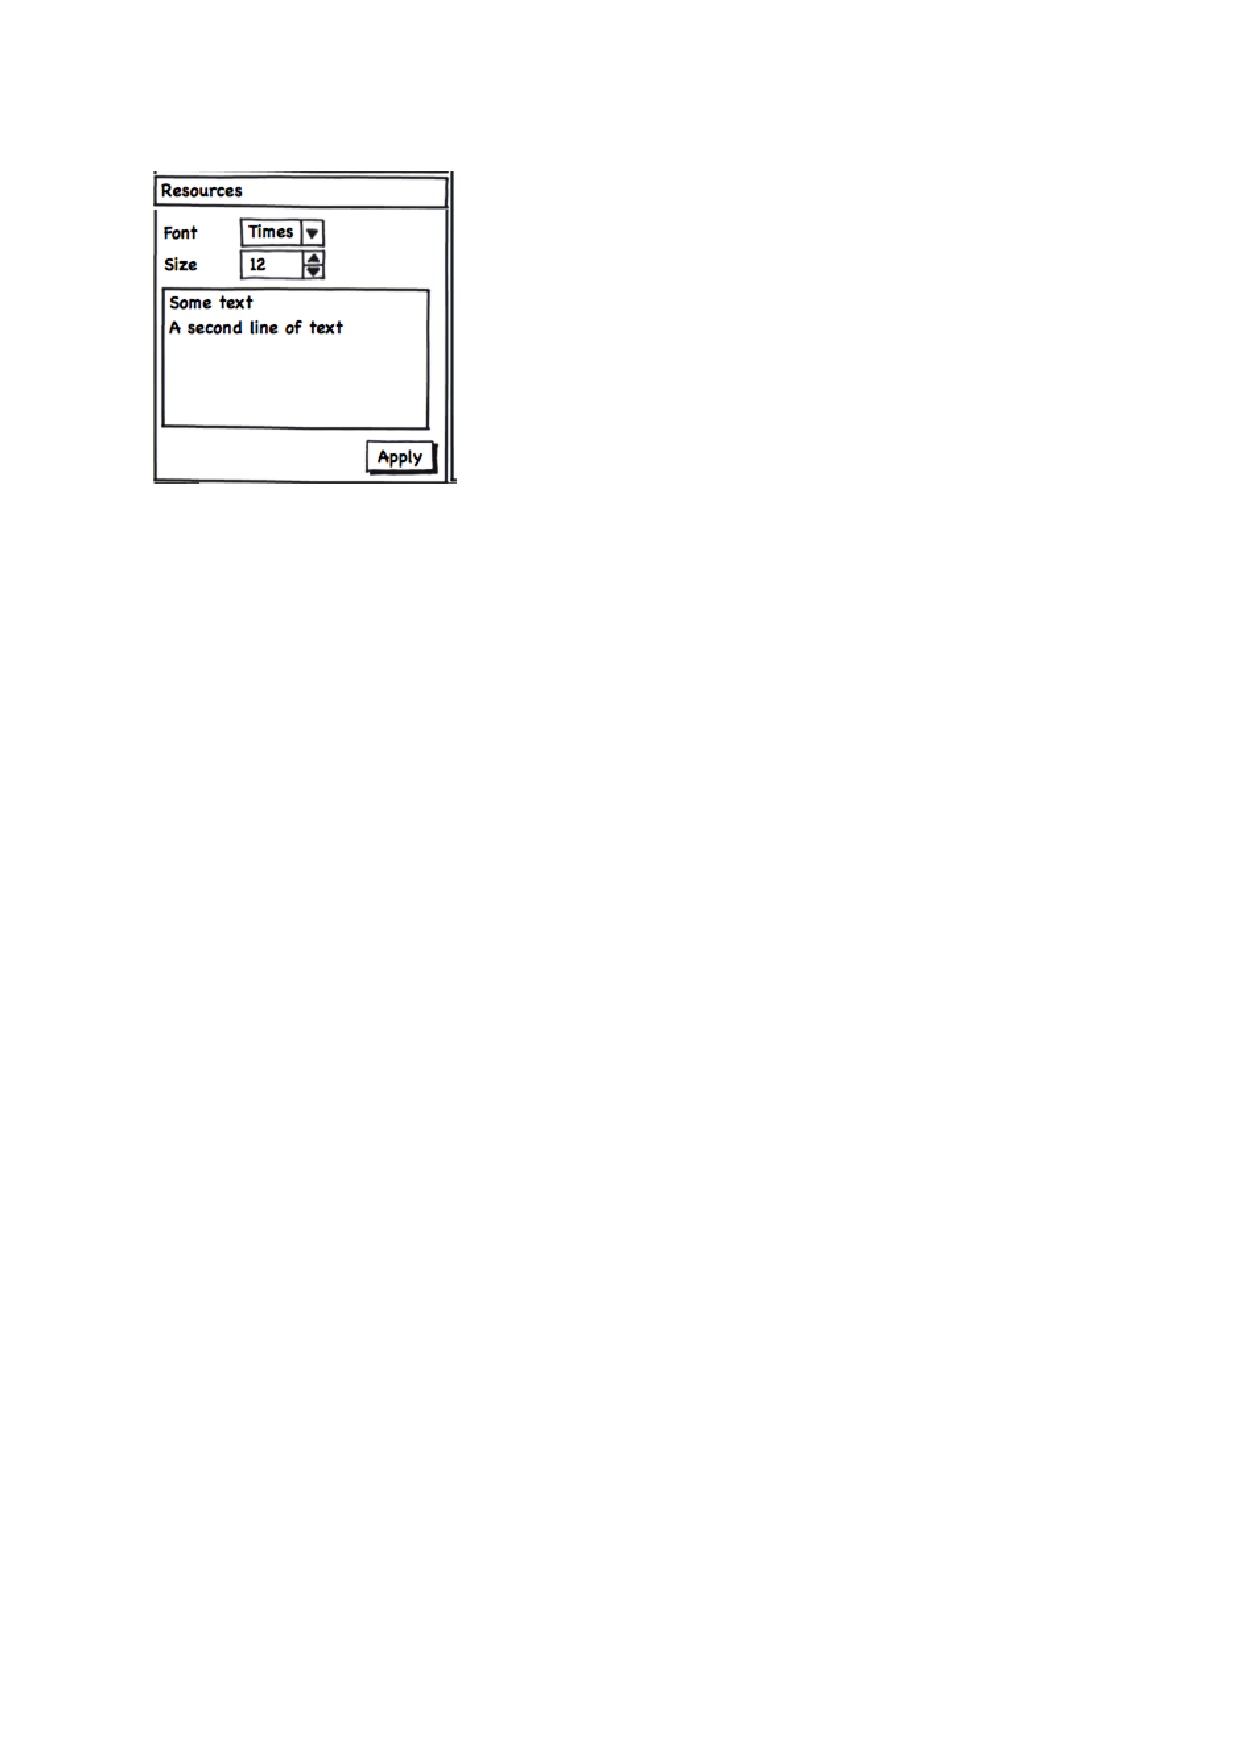
\includegraphics[scale=.8]{chap1/img-12}}& \parbox{271pt}{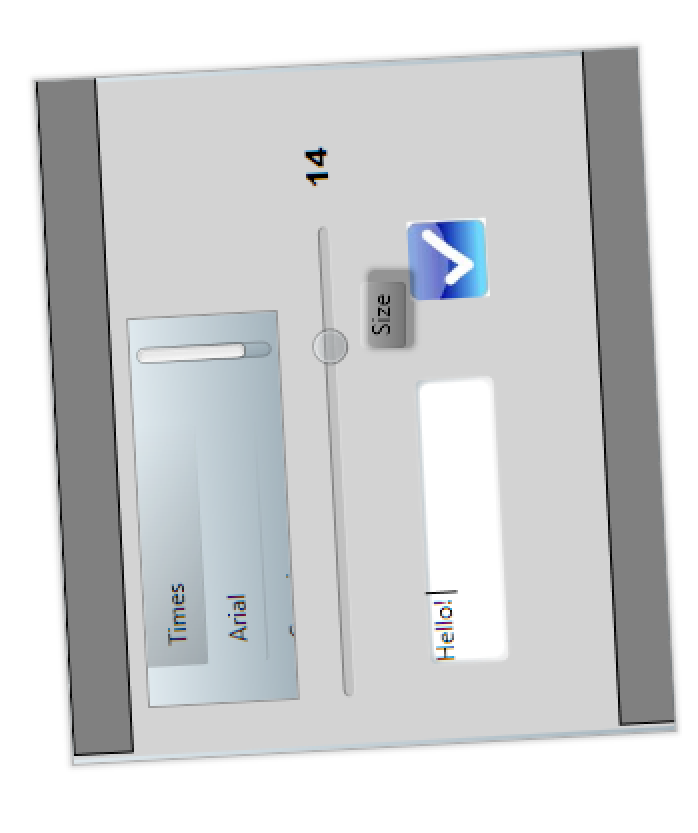
\includegraphics[angle=270, scale=.5]{chap1/img-13}}\\
\hline
\end{tabular}
\vspace{3pt}
\caption{Migration de l'aspect visuel d'un formulaire}
\label{tab:chap2:1}
\end{center}
\end{table}


\subsubsection{Synth�se des guidelines pour la migration d'UI vers les tables interactives}
\label{sec:chap2:3:5:5}
Le corpus de guidelines d�crit dans la section~\ref{sec:chap2:3:5} sont des recommandations de haut niveau utiles et n�cessaires pour la migration des UI vers une table interactive. Cette caract�risation de ce corpus a pour but de rendre une UI de d�part tangible et collaborative pendant la migration tout en consid�rant les autres modes d'interactions des tables interactives et les aspects visuels de l'UI.

Les liens entre ces guidelines peuvent �tre synth�tis�s � l'aide du diagramme de la figure~\ref{fig:chap2:21} qui pr�sente les trois cat�gories de guidelines, les 7 guidelines pour les UI tangibles et collaboratives et les liens entre ces guidelines. Dans la cat�gorie des guidelines pour TUI, les guidelines G2 (Objets physiques tagu�s) et G3 (Forme des objets Physiques) sp�cifient les moyens d'interactions tangibles � choisir et � associer aux objets virtuels identifi�s par la guideline G1. 

Dans la cat�gorie des guidelines pour UI collaborative, la guideline nombre d'utilisateurs (G4) est sp�cifi�e pour les apects li�s aux t�ches par la guidelines de couplage des t�ches et utilisateurs (G5), la guideline sp�cifiant le partage de l'espace de travail (G6) entre les utilisateurs et la guideline pr�conisant l'utilisation 360� de l'UI (G7) permet l'accessibilit� de l'UI pour tous les utilisateurs autour de la table.

Dans la cat�gorie comportant les autres guidelines pour les UI sur surface nous regroupons deux sous cat�gories; la premi�re concerne les interactions tactiles et la seconde le style de l'UI migr�e.
\begin{figure}[h]
\begin{center}
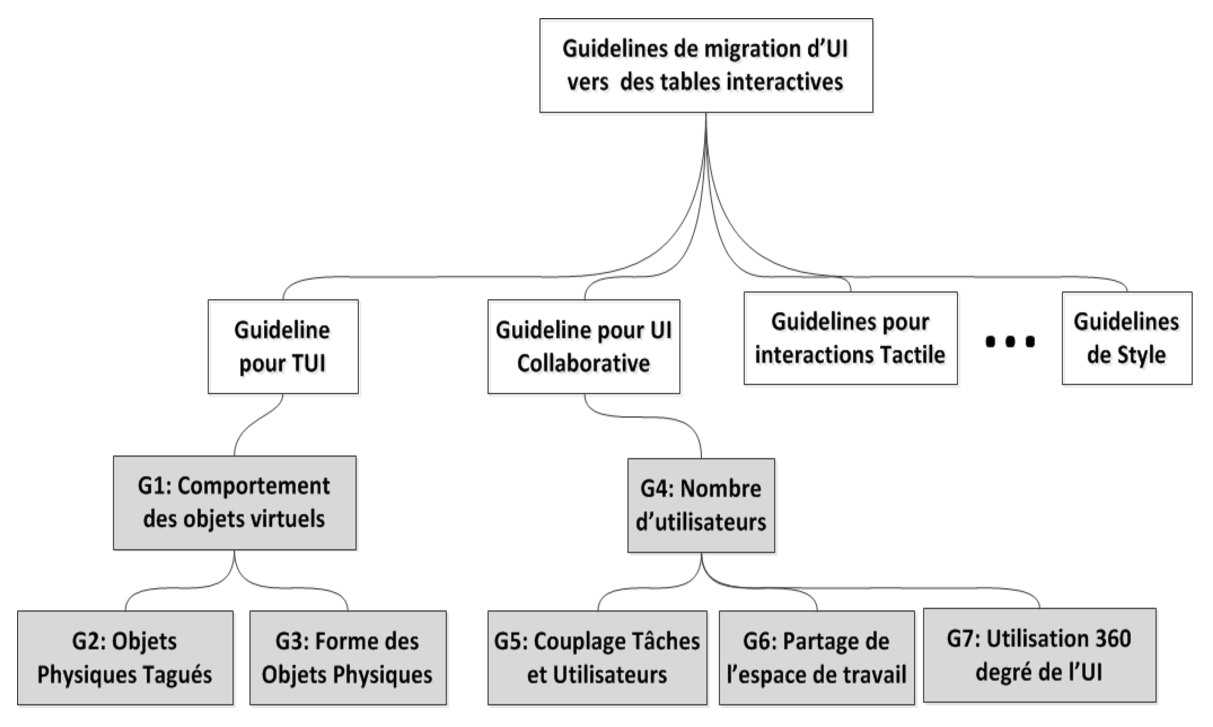
\includegraphics[angle=270, width=450pt]{chap2/img-23-1}
\caption{Liens entre les guidelines de migration d'une UI vers les tables interactives}
\label{fig:chap2:21}
\end{center}
\end{figure}

\section{Concepts pour la migration d'UI}
\label{sec:chap2:4}
Dans les sections pr�c�dentes, nous avons identifi� quels sont les probl�mes li�s � la migration d'UI vers une table interactives en partant d'un exemple d'application (� la section~\ref{sec:chap2:2}). Ensuite nous avons aussi identifi� les sp�cificit�s des tables interactives qui sont importantes pour la migration des UI � travers ses propri�t�s caract�ristiques et les guidelines. Dans cette section nous abordons les probl�matiques li�es aux architectures des applications � migrer et les mod�les d'interactions abstraites pour d�crire des �quivalences entre les modalit�s d'interactions.

\subsection{Architecture des applications � migrer}
\label{sec:chpa2:4:1}
Les applications � migrer sont des syst�mes interactifs (SI) con�us en respectant un mod�le d'architecture. Les mod�les d'architectures sont des patrons de conception logiciel, ils  pr�conisent des strat�gies de r�partition des services qui se traduisent par un ensemble de constituants logiciels. En g�n�ral, la d�composition minimale des SI pr�conise une s�paration entre le Noyau Fonctionnel (NF) et ceux de l'UI. Dans cette section nous pr�sentons deux mod�les d'architectures, d'abord le mod�le ARCH~\cite{UIMS1992} qui se base sur des composants logiciels sp�cifiques et ind�pendants des plateformes, ensuite le mod�le MVC~\cite{Krasner1988} .

\subsubsection{ARCH}
ARCH~\cite{UIMS1992} est un mod�le d'architecture qui se base sur des composants conceptuels du mod�le de Seeheim~\cite{Pfaff1985}. Comme l'indique la figure~\ref{fig:chap2:5}, ce mod�le permet une s�paration entre le NF, le Contr�leur de Dialogue (CD) et la Pr�sentation. Les deux pieds de l'arche sont des composants sp�cifiques � une plateforme; le composant NF d�crit un domaine pr�cis et les composants d'Interaction sont li�s � des dispositifs du monde r�el. Le CD g�re l'enchainement des t�ches ainsi que les liens avec les objets des deux composants voisins. L'Adaptateur de domaine joue un r�le d'interface avec le composant NF pour corriger les diff�rences de conceptions. Le composant Pr�sentation est une bo�te � outils virtuelle, telle que XVT~\cite{Valdes1989} qui impl�mente les objets de pr�sentations concr�tis�s finalement par les objets d'interaction de la biblioth�ques graphique. 
%PAC-Amodeus~\cite{Nigay1994} est un mod�le d'architecture bas� sur ARCH, il permet de d�finir plusieurs contr�leurs de dialogue pour une application gr�ce aux agents  PAC.  
\begin{figure}[h]
\begin{center}
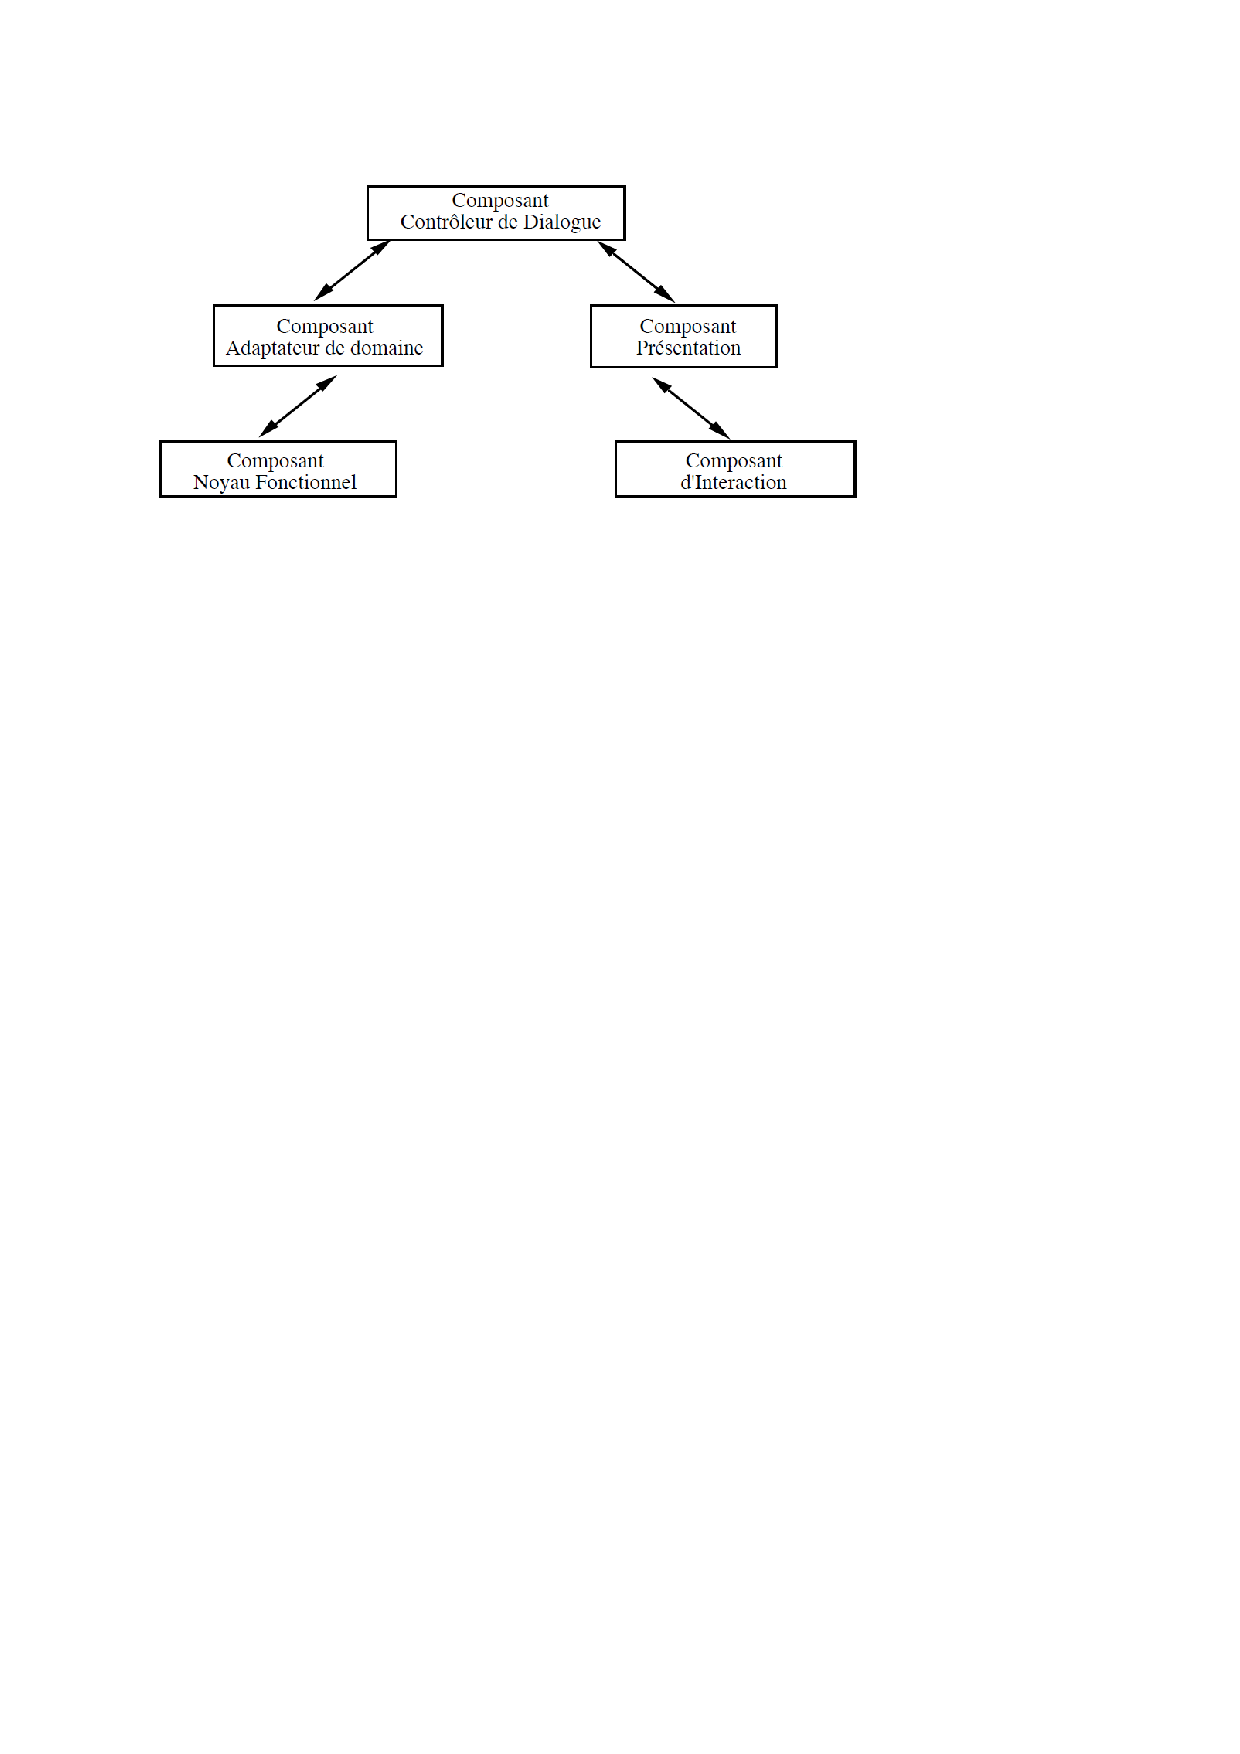
\includegraphics[width=340pt]{chap2/img-7}
\caption{Composants du mod�le ARCH}\label{fig:chap2:5}
\end{center}
\end{figure}

\paragraph{Migration d'une application respectant une architecture ARCH}-
Thevenin et al.~\cite{Thevenin2002} se basent sur l'architecture ARCH pour concevoir des applications avec des UI multi cibles et adaptables. Dans le cadre de la migration, cette approche consiste � remplacer les composants des interacteurs logiques et physiques de l'UI � migrer pour qu'ils soient conformes aux principes de conception de la table interactive cibl�e.

La migration des interacteurs physiques concerne la migration du composant d'interaction du mod�le ARCH~\cite{Thevenin2002}. Elle consiste en un changement de biblioth�que graphique de l'application de d�part et � utiliser celle de la plateforme d'arriv�e. Ce type de migration permet de conserver la nature des composants graphiques mais leurs rendus sont distincts en fonction des plateformes et des biblioth�ques graphiques. En consid�rant l'application CBA par exemple, la nature des �l�ments logiques de l'UI d�crits dans le composant Pr�sentation tels que Bouton, Liste d'images, etc. sont interpr�t�s en fonction des biblioth�ques graphiques (DiamondSpin, Surface SDK, etc.).

La migration des interacteurs physiques permet certes d'utiliser la biblioth�ques graphique de la plateforme d'arriv�e mais elle ne prend pas en compte les guidelines de la plateforme cibl�e.\\
\fbox{\parbox{0.9\textwidth}{ En effet en migrant les interacteurs physiques de l'UI CBA desktop par les �l�ments de la bo�te � outils d'une table interactive sans prendre en compte les guidelines pour les TUI ou les UI collaboratives, le layout et les interactions de UI r�sultantes par exemple ne seront pas conformes aux sp�cificit�s de la table interactive cibl�e.}}

\paragraph{Prise en compte des principes de conceptions}- 
Dans le cadre de la migration d'une application respectant le mod�le d'architecture ARCH~\cite{Pfaff1985}, les guidelines identifi�es � la section~\ref{sec:chap2:3:5} sont utiles pour transformer le Composant de pr�sentation et pour la g�n�ration du composant d'interaction en permettant par exemple la s�lection des composants graphiques. En consid�rant l'UI CBA et les guidelines pour UI collaboratives, la guideline pour le partage d'espace de travail (G6) permet par exemple de r�organiser le layout de l'UI CBA en transformant le composant de pr�sentation et la guideline d'utilisation 360 degr� permet de choisir des panels avec des mouvements de rotation, de d�placement pendant la g�n�ration du composant d'interaction. 


\subsubsection{MVC}
MVC~\cite{Krasner1988} est un mod�le d'architecture pour la conception des syst�mes interactifs r�utilisables. Il divise les applications en trois types de composants : le mod�le(M), la vue(V) et le contr�leur(C). Le mod�le est une repr�sentation du domaine d'une application, il peut contenir des donn�es, des services, etc. et il fait partie du NF d'une application. La vue est la structure de l'UI d'une application, elle est constitu�e des �l�ments d'une biblioth�que graphique. Le contr�leur est une interface entre le mod�le, la vue et les dispositifs d'interactions en entr�e.

\paragraph{Migration d'une application respectant une architecture MVC}-
En consid�rant une partie de l'UI de l'application CBA, la figure~\ref{fig:6} repr�sente des instances des diff�rents �l�ments du mod�le MVC. La vue est compos�e de \textit{JPanel, JLabel, JComboBox} et d'une \textit{JList} contenant des images. La s�lection d'une cat�gorie du s�lecteur \textit{JComboBox}  avec un clavier ou une souris modifie la liste d'images en faisant d'abord appel au contr�leur de \textit{JComboBox} ensuite au mod�le de JList pour mettre � jour la vue.
La migration de cet art�fact d'UI vers une table interactive qui supporte la biblioth�que graphique DiamondSpin par exemple implique la modification de la vue en rempla�ant les composants graphiques par leurs �quivalents et en adaptant le code du contr�leur et du mod�le pour remplacer les variables correspondant aux composants graphiques de la vue. Par exemple dans le cas o\`{u} \textit{DSComboBox} correspond � \textit{JComboBox} dans DiamondSpin, le type de la variable \textit{cb} du contr\^{o}leur doit \^{e}tre remplac� dans le contr\^{o}leur et le mod\`{e}le.

Par cons�quent, la migration de l'UI vers la table interactive avec cette hi�rarchie implique une modification � la fois du contr\^{o}leur, de la vue et du mod\`{e}le. Pour �viter ces modifications, il faut que le code des applications � migrer respecte des heuristiques qui favorisent la r�utilisation des diff�rents composants de l'application. Parmi ces heuristiques on peut citer: la s�paration entre les �l�ments sp�cifiques � la plateforme (PSM) et les �l�ments ind�pendants de la plateforme (PIM) au niveau du contr\^{o}leur et de la vue d'une part, et la non utilisation des �l�ments PSM du contr�leur de la vue au niveau du mod�le d'autre part. Cette s�paration permettra de changer les contr\^{o}leurs de dialogue sp�cifiques aux dispositifs d'interaction et les vues sp�cifiques aux biblioth\`{e}ques graphiques.
\begin{figure}[h]
\begin{center}
\includegraphics[width=432pt]{chap2/img-2.eps}
\caption{Mod�le Vue Contr�leur}\label{fig:6}
\end{center}
\end{figure}

La prise en compte guidelines pendant la migration des �l�ments du mod�le MVC con�us en respectant les heuristiques pr�conisant de s�paration PIM et PSM se fait comme pour les composants du mod�le d'architecture ARCH.

\subsubsection{R�sum�}
Nous avons pr�sent� dans cette section~\ref{sec:chpa2:4:1} le mod�le d'architecture de ARCH  qui permet la migration des composants de l'UI sans modification des composants du NF. Le mod�le d'architecture ARCH facilite aussi la prise en compte des guidelines pendant la migration. Par ailleurs, En consid�rant un mod�le d'architecture MVC avec des composants qui respectent une s�paration entre les �l�ments PSM et les �l�ments PIM, il est possible de migrer les composants d'UI sans modifier les composants du NF et aussi de prendre en compte les principes de conception pendant la migration. Le mod�le MVC permet en une s�paration entre les interactions en entr�e d�crites au niveau des contr�leurs et les interactions en sortie. Cette s�paration facilite le \textbf{changement des interactions} en entr�e. 


\subsection{Mod�le d'interactions abstraites}
\label{sec:chap2:4:2}
La migration d'une UI desktop  vers les tables interactives est un processus qui implique un changement de modalit� d'interaction tel que nous l'avons montr� � la section~\ref{sec:chap2:3:3}. Le \textbf{changement des modalit�s d'interactions} doit pr�server les actions de l'UI de d�part et l'adapter aux dispositifs d'interactions de l'UI d'arriv�e. 
Le changement de modalit�s d'interactions est possible en d�crivant des �quivalences entre les diff�rentes modalit�s d'interactions d'une UI. Ce qui peut se faire en se basant sur un mod�le ind�pendant des dispositifs d'interactions.

\fbox{\parbox{0.9\textwidth}{Le mod�le d'interactions abstraites permet de d�crire des �quivalences entre deux modalit�s d'interactions en jouant un r�le de langage pivot. }}

Dans cette section nous pr�sentons deux mod�les d'interactions abstraites et nous en d�duirons quelques caract�ristiques d'un mod�le d'interactions abstraites pour la migration.
 
\subsubsection{Mod�le de Vlist}
Vlist et al. ~\cite{Vlist2011} proposent les primitives d'interaction (\textit{interaction primitives}) qui constituent les plus petits �l�ments d'interactions adressables ayant une relation significative avec l'interaction elle-m�me. Selon eux, il est possible de d�crire les capacit�s d'interactions des dispositifs d'interactions  � l'aide des primitives d'interactions et ensuite la relation entre les dispositifs et l'UI sera d�crite en faisant un mapping s�mantique. Les primitives d'interactions sont associ�es � chaque dispositif d'interaction, elles sont choisies, identifi�es et associ�es aux dispositifs par le concepteur de l'UI. Par exemple les primitives d'interactions Up, Down correspondent aux touches �tiquet�es '+' et '-', ces primitives d'interactions ont des types de donn�es et des valeurs, elles sont mapp�es sur des composants graphiques tels que les contr�les de volume pour permettre l'utilisation de composants avec ces touches. L'objectif de ce mapping s�mantique est de faciliter son adaptation en fonction des contextes.

Dans le cadre de la migration, la mise en correspondance des dispositifs d'interactions des plateformes de d�part et d'arriv�e semble �tre possible en utilisant une description s�mantique des capacit�s des dispositifs d'interaction d'une plateforme par les primitives d'interactions. Pour cela les primitives d'interactions doivent pouvoir d�crire tous les dispositifs d'interactions en se basant sur un seul vocabulaire. En effet Up et Down sont certes adapt�s pour les touches '+' et '-' mais en consid�rant un �cran tactile par exemple il faut d�crire les diff�rents types de contacts (simple, double, multiple, toucher et glisser, etc.).
\subsubsection{Mod�le de Gellersen}
Gellersen~\cite{Gellersen1995}  quant � lui propose un mod�le d'interactions abstraites qui a pour but de d�crire les interactions en entr�e et en sortie ind�pendamment des modalit�s d'interactions. Ce mod�le est aussi ind�pendant d'un domaine ou d'une application. Il est pr�sent� � la figure \ref{fig:chap2:15} et il d�crit une hi�rarchie des interactions en entr�e et en sortie. Les interactions en entr�e sont raffin�es en deux cat�gories, les interactions d'entr�e de donn�es telles que \textit{Editor, Valuator} (�diter du texte) et \textit{Option} (s�lectionner un �l�ment d'une liste) qui sont des sous classes de \textit{Entry} d'une part et les interactions de \textit{Command}\footnote{les Command sont des interactions en entr�e de contr�le avec des param�tres (exemple copier texte, coller texte, etc.)} et de \textit{Signal}\footnote{Les Signal sont des interactions en entr�e sans param�tres (exemple valider)} d'autre part. Les interactions en sortie sont aussi de deux types : les messages (alertes, confirmation, etc.) et la vue qui permet l'affichage des donn�es et des composants de l'UI. 

\begin{figure}[h]
\begin{center}
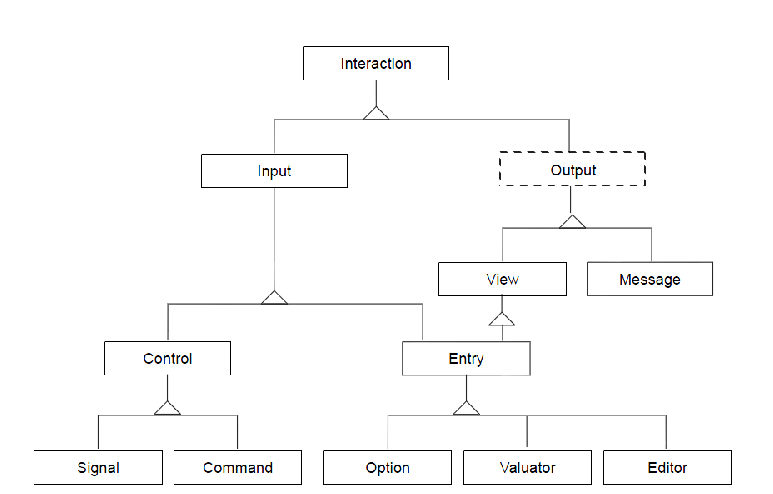
\includegraphics[width=353pt]{chap2/img-5.eps}
\caption{Mod�le d'interactions abstraites de Gellersen}\label{fig:chap2:15}
\end{center}
\end{figure}


Dans le cadre du changement de modalit� d'interaction entrain� par la migration, ce mod�le permet de d�crire les interactions des diff�rents composants 
graphiques de l'UI de mani�re ind�pendante des modalit�s d'interactions. Par exemple une fen�tre d'authentification comportant des champs de texte et des boutons, les champs de texte seront repr�sent�s par les Editor qui sont des interactions � la fois en entr�e et en sortie et les boutons seront repr�sent�s par des Command dans un mod�le abstrait. 

Ce mod�le identifie � la fois les interactions en entr�e et en sortie de haut niveau et ind�pendamment des modalit�s d'interactions. Dans le cadre de la migration de l'UI CBA par exemple, les interactions telles que la rotation, le d�placement ou le redimensionnement qui sont li�s aux guidelines de la table interactives doivent �tre interpr�t�s comme des commandes. Cette interpr�tation n'est pas g�n�rique et d�pend du concepteur des interactions,  en effet le d�placement peut �tre consid�r� comme une rotation en modifiant l'angle par exemple. De mani�re g�n�rale, le mod�le de Gellersen est un mod�le d'interactions abstraites qui n�c�ssite la sp�cification de certaines interactions ind�pendantes des modalit�s d'interactions pendant la migration.


\subsubsection{R�sum�}
\fbox{\parbox{0.9\textwidth}{
Deux caract�ristiques sont essentielles pour les mod�les d'interactions abstraites : 
\begin{itemize}
\item leurs ind�pendances d'une modalit� d'interaction 
\item et leur capacit� � d�crire toutes interactions du langage d'une modalit�. 
 \end{itemize}
}}

\section{Conclusion}
\label{sec:chap2:5}
Dans ce chapitre nous avons �tudi� les probl�mes li�s � la migration d'UI vers une table interactive qui consiste �:
\begin{itemize}
\item transformer le layout de l'UI de d�part conform�ment aux guidelines pour les UI collaboratives
\item changer les modalit�s d'interactions de l'application de d�part conform�ment aux guidelines pour les UI tangibles et tactiles
\item adapter la taille et le style de l'UI de d�part aux recommandations de la plateforme d'arriv�e.
\end{itemize}

Dans le chapitre suivant, nous �tudions quelques m�canismes de migration des UI en faisant ressortir les probl�matiques li�es � la prise en compte des guidelines et au changement de modalit�s d'interactions de ces m�canismes de migration.
	
	\chapter{Tables interactives et Migration des UI}
	%\label{chap3}
	%\minitoc
	%\section{Introduction}

\label{sec:chap3:0}

La migration des applications est une activit� de d�placement et d'adaptation d'un logiciel d'un environnement source vers un environnement cible. Elle est plus globale que le portage d'application  ~\cite{Mooney1995} car elle ne se limite pas qu'au changement de langages de programmation ou au changement des syst�mes d'exploitation. La migration englobe les probl�matiques de r� engineering, de reverse engineering, de forward engineering et de portage d'applications. McClure et al.~\cite{McClure1992} d�finissent le r� engineering comme une am�lioration d'un syst�me existant pour le rendre conforme aux standards. Le reverse engineering consiste � analyser un syst�me existant pour d�crire la repr�sentation d'origine de mani�re plus abstraite~\cite{McClure1992}. Le forward engineering est une concr�tisation de la repr�sentation abstraite d'un syst�me dans une impl�mentation. Une approche de migration d'UI vers une table interactive implique un r� engineering de l'UI source en impliquant d'abord une phase de reverse engineering de l'UI source ensuite une phase de forward engineering.

Dans notre contexte, les SI � migrer ont une d�composition fonctionnelle minimale qui comprend une UI et un NF. Cette d�composition facilite la migration de l'UI en r�utilisant le NF de l'application de d�part par exemple. Les solutions de migration d'UI d'une application qui prennent en compte les guidelines de la plateforme cible peuvent �tre manuelles et sp�cifiques dans le cas o� le concepteur se charge de transformer l'UI de d�part pour la plateforme cible. Ces solutions peuvent aussi �tre automatis�es par des processus qui se basent sur des mod�les et des principes g�n�riques pour une classe d'applications ou de plateformes. 

Nous pr�sentons dans ce chapitre des approches de migration d'UI dans le but de savoir comment sont adapt�s les diff�rents aspects des UI par ces approches de migration. Pour r�pondre � cette question, nous nous basons sur trois crit�res importants pour d�finir une solution r�utilisable pour la migration d'UI vers les tables interactives.
\begin{enumerate}
\item \textbf{Les �quivalences} entre les dispositifs d'interactions, les biblioth�ques graphiques des plateformes source et cible. 
\item \textbf{La mod�lisation} des diff�rents aspects des UI : Structure, Interactions, Comportement, Layout, Style.
\item La prise en compte des \textbf{Guidelines} par les m�canismes de migration d'UI pour garantir une UI conforme aux crit�res d'utilisabilit�.
\end{enumerate}


Dans ce chapitre, la section~\ref{sec:chap3:1} pr�sente les approches de migration sp�cifiques � des applications ou � des bo�tes � outils. La section~\ref{sec:chap3:3} pr�sente les approches de migration d'UI bas�es sur des mod�les d'UI. La section~\ref{sec:chap3:3} fait une synth�se des diff�rentes approches de migration d'UI et pr�sente les objectifs de notre solution.


\section{Approches sp�cifiques de migration d'UI }
\label{sec:chap3:1}

Dans cette section nous �tudions les processus de migrations sp�cifiques � une
application ou � une bo�te � outils. Nous pr�sentons d'abord un processus qui
permet de migrer manuellement une application sp�cifique (AgilePlanner) sur une
table interactive, ce processus identifie des guidelines pour les
UI collaboratives et s'appuie sur une d�marche structur�e. Ensuite nous
pr�sentons une famille de m�canismes de migration d'UI des applications
existantes sur les tables interactives sans re conception de l'UI de d�part.


\subsection{Migration de l'application AgilePlanner vers une table interactive}

\label{sec:chap3:1:1}

C'est un processus manuel et ad hoc mis en place pour la migration de l'application AgilePlanner\footnote{AgilePlanner est une application de planification et de gestion de projet suivant la m�thode Agile. Sur une table interactive, elle est utilis�e pour faire du brainstorming dans le cadre de plannings de projets par exemple} vers une table interactive~\cite{Wang2008}. Le processus mis en place �tait bas� sur quatre phases. 

La premi�re phase consistait � analyser l'UI de l'application � migrer, elle permettait d'identifier les diff�rentes zones (menu, l�gendes, zones d'interaction, espace de travail, etc.). 

La deuxi�me phase consistait � �valuer l'UI de l'application � migrer sur une table interactive, le but de cette �valuation �tait de ressortir les diff�rences entre desktop et table interactive dans le but d'en d�duire des recommandations qui seront des guidelines pour le concepteur. Il en est ressorti les 7 guidelines suivantes:

\begin{itemize}

\item Avoir des composants d'UI de l'application d�pla�ables et utilisables en 360� 

\item Utiliser la reconnaissance gestuelle pour les interactions utilisateurs et �viter les menus traditionnels

\item Utiliser l'�criture � main lev�e au lieu du clavier pour la saisie des textes

\item Prendre en compte les interactions concurrentes pendant la conception de l'UI

\item Pouvoir utiliser des composants graphiques de taille assez grande pour faciliter les interactions tactiles

\item �viter l'utilisation des bo�tes de dialogues pop up

\item Permettre � l'UI de l'application de s'adapter aux diff�rentes tailles des tables interactives.

\end{itemize}
Ces guidelines sont conformes aux guidelines pour les UI collaboratives et aux guidelines pour les interactions tactiles que nous avons pr�sent�es au chapitre pr�c�dent (cf. section~\ref{sec:chap2:3:5}).

La troisi�me phase consistait � appliquer les guidelines de la phase pr�c�dente pour concevoir � nouveau une UI de l'application AgilePlanner utilisable sur table interactive. Certaines des guidelines telles que la rotation et le d�placement des composants graphiques, l'�criture � main lev�e, les reconnaissances gestuelle et vocale �taient fournies par l'environnement logiciel de certaines tables interactives.

La derni�re phase du processus consistait � �valuer l'UI produite en demandant aux utilisateurs finaux d'�valuer l'utilisabilit� de chaque fonctionnalit� migr�e de l'application AgilePlanner. L'UI migr�e a �t� modifi�e par rapport aux remarques issues des �valuations. Enfin l'UI a �t� r��valu�e � nouveau pour mesurer la satisfaction des testeurs. Les r�sultats de cette r��valuation ont montr� que l'utilisabilit� de l'�criture � main lev�e sur la table interactive peut �tre am�lior�e.

La migration manuelle  d'une UI est un processus qui comporte plusieurs phases. Dans cette section nous avons pr�sent� une approche qui nous permet d'identifier quatre phases importantes:

\begin{enumerate}

	\item Analyser l'UI de d�part pour identifier la structure des �l�ments qui la compose et ses fonctionnalit�s
	\item Identifier les guidelines qui permettront la migration: cet identification se fait en se basant sur les diff�rences entre la plateforme de d�part et celle d'arriv�e
	\item Appliquer les guidelines pour migrer l'UI de d�part
	\item �valuer  et am�liorer le r�sultat obtenu.

\end{enumerate}


\subsubsection{R�utilisation du processus pour d'autres applications}
\label{sec:chap3:1:1:1}
Les �tapes du processus de migration de l'application AgilePlanner vers une table interactive et la mise en \oe{}uvre des guidelines identifi�es constituent des ``savoir faire'' qu'un d�veloppeur souhaiterais r�utiliser pour d'autres applications. 

Les m�canismes d'adaptation de l'application AgilePlanner ne peuvent pas �tre r�utilis�s pour d'autres applications car ils sont sp�cifiques  � cette application. En effet, l'analyse et l'identification des diff�rentes zones de l'UI ne s'appuient pas sur des \textbf{mod�les ind�pendants de la plateforme}.

La mise en \oe{}uvre des guidelines identifi�es dans ce processus est bas�e sur l'\textbf{intuition}. Nous avons consid�r� l'UI de deux applications: l'application CBA et l'UI d'une application agenda pr�sent�e � la figure~\ref{fig:chap3:6}. En appliquant les guidelines identifi�es � la section~\ref{sec:chap3:1:1} pour migrer ces deux UI. En ce qui concerne l'application agenda,  les composants graphiques repr�sentant la barre de menu, la barre de recherche, la liste de cat�gorie et le tableau peuvent �tre tous d�pla�ables sur la table ou bien  l'on peut consid�rer la liste des cat�gories et le tableau de contacts comme �tant ensemble. Dans le cas de l'application CBA, le choix des groupes utilisables � 360� peut se faire comme le propose la figure~\ref{fig:chap2:18} par exemple.
 
Nous remarquons que l'utilisation des guidelines pour deux applications distinctes d�pend de l'\textbf{interpr�tation} faite par les personnes en charge de la migration car ces guidelines ne pr�cisent pas formellement comment on peut regrouper les composants graphiques d�pla�ables par exemple.

\begin{figure}[h]

\begin{center}

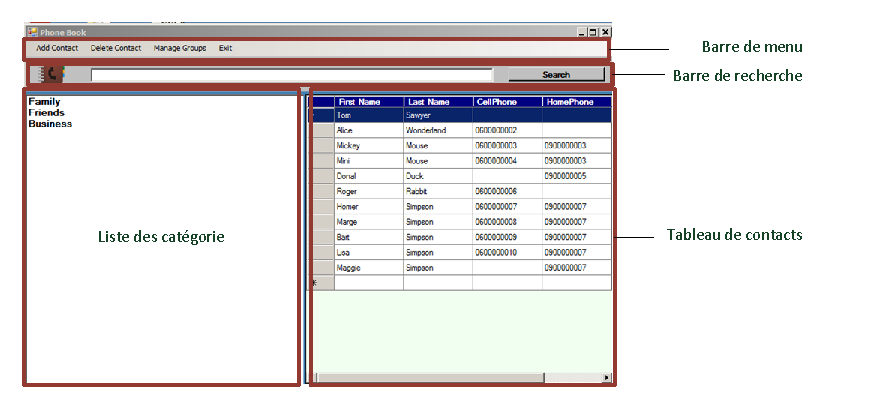
\includegraphics[scale=1]{chap3/img-12}

\caption{Application de consultation des contacts }

\label{fig:chap3:6}

\end{center}

\end{figure}

\subsubsection{R�sum�}
Les m�canismes de migration du processus d�crits dans cette section, tels que les �quivalences des composants graphiques ou des dispositifs d'interactions des plateformes source et cible sont manuels. Et les m�canismes de prise en compte de guidelines sont aussi manuels et bas�s sur les \textbf{connaissances} des personnes en charge de la migration. 

\fbox{\parbox{0.9\textwidth}{
Par ailleurs si l'on souhaite r�utiliser ce m�canisme de migration d'UI, il est
indispensable de formaliser les guidelines en s'appuyant sur des mod�les ind�pendants des plateformes source et cible (tels qu'un menu, un formulaire, etc.) et en d�crivant des r�gles de transformations des mod�les d�crivant les aspects de l'UI concern�s par la migration (layout, interactions, styles, etc.)}}


\subsection{Portage des applications existantes sur des tables interactives }
\label{sec:chap3:1:2}
Cette approche~\cite{Besacier2010} a pour but de r�utiliser des applications pour desktop sur une table interactive sans reconception de l'UI, l'objectif est d'adapter les diff�rents moyens d'interactions (clavier et souris) des desktops sur une table interactive DiamondTouch en utilisant plusieurs types de technologies. 
L'approche regroupe des technologies qui prennent en compte des guidelines li�es � la conception des UI collaboratives. Besacier~\cite{Besacier2010} a caract�ris� six technologies qui permettent la r�utilisation des applications existantes sur une table interactive.

\paragraph{La capture d'�cran }est une technologie qui consiste � prendre une capture de l'�cran de l'UI de d�part � intervalle r�gulier, la capture d'�cran enregistre une copie exacte de l'image affich�e sur l'�cran du desktop dans une zone m�moire o� elle peut �tre modifi�e pour �tre adapt�e � l'environnement de la table interactive. Cette approche se situe dans un contexte de portage des applications existantes. Elle ne permet pas de porter des interactions en entr�e car l'UI port�e est constitu�e d'images captur�es et ces images ne contiennent pas de m�ta donn�es. 
\paragraph{La carte graphique virtuelle} est une am�lioration de la technologie bas�e sur la capture d'�cran. L'approche utilise le serveur Metisse~\cite{} qui stocke les fen�tres de l'application de d�part sous forme d'images.  Le serveur Metisse joue un r�le de carte graphique virtuelle car il redessine les fen�tres sur l'�cran de la table interactive � travers un compositeur et il redirige les �v�nements venant d'une souris ou d'un clavier vers l'application. Cette technologie permet de porter les fen�tres des applications desktops sur une table interactive en offrant la possibilit� aux utilisateurs de les manipuler facilement. Cependant les composants graphiques des fen�tres port�es ne sont pas interactifs car ils restent des images de l'UI de d�part.

\paragraph{L'�mulation du clavier et de la souris} est une technologie qui am�liore les deux technologies pr�sent�es ci-dessus. Elle permet de porter aussi les interactions en entr�e (du clavier et de la souris). Cette technologie se base sur des techniques qui permettent d'utiliser plusieurs pointeurs avec applications Java existante~\cite{}.  Les probl�mes li�s aux passages d'une UI mono utilisateur � une UI multi utilisateurs sur la table interactive sont partiellement r�solus par cette approche. En effet, la technique permet de porter plusieurs applications � la fois sur une table interactive et � chaque application est associ�e un utilisateur avec son clavier et sa souris virtuels. Dans le cas d'une UI mono utilisateur que l'on souhaiterait utiliser en multi utilisateurs, cette technique ne permet pas de multi touches simultan�es car l'interaction d'un utilisateur verrouille la table � d'autres utilisateurs d'une m�me application.

\paragraph{Le langage de script }est une technologie qui permet de porter des UI des applications existantes sur une table interactive en r�solvant les limites li�es aux multi touches et multi utilisateurs de la technologie pr�c�dente. Le langage de script est sp�cifique � une application et consiste � �crire dans un sc�nario un ensemble de scripts qui font appel chacun � une fonctionnalit� de l'application � porter. Les scripts sont appel�s par une application de table interactive qui capture les �v�nements en entr�e de la table et les associes � un script pr�cis. Par exemple pour afficher un fichier sur la table, l'application table interactive associe un script d'ouverture et de lecture de fichiers de l'application de d�part � l'�v�nement lanc� apr�s la pause d'une feuille de papier sur la table interactive. Cette technique n'est pas facilement r�utilisable pour d'autres applications car les scripts sont �crits en fonction des applications. Les donn�es �chang�es entre l'application � migrer et l'application table interactive sont d�crites dans un mod�le. Ce mod�le de donn�es permet de faire le mapping entre les donn�es issues des composants graphiques de l'application � miger et les composants graphiques (DiamondSpin) de la table interactive. Les guidelines de la m�taphore du papier\footnote{d�placement, rotation, redimensionnement, changement d'�chelle, pliage}~\cite{Besacier2007} sont prises en compte dans l'impl�mentation de cette approche qui consid�re la biblioth�que graphique DimaondSpin de la table DiamondTouch. Cette prise en compte des guidelines d�pend fortement des connaissances et de l'intuition du concepteur en charge du portage.

\paragraph{Les API d'accessibilit� num�rique}\footnote{ Elles sont utilis�es pour offrir des interfaces alternatives � des groupes d'utilisateurs sp�cifiques, par exemple des utilisateurs souffrant de d�ficience visuelle} permettent d'obtenir des informations s�mantiques � propos des UI graphiques en cours d'ex�cution. Ces informations constituent des instances de mod�les de structure d'une UI donn�e (comprenant les composants graphiques, les donn�es, les positions, etc.). Ce mod�le permet de d�crire une technique de migration qui segmente les images obtenues par capture d'�cran de l'UI source. Les parties de l'UI de d�part peuvent donc �tre dupliqu�es ou juxtapos�es en se basant sur le mod�le de structure et les images segment�es. Le mod�le de structure et les images segment�es sont les �l�ments de l'UI source qui permettent de g�n�rer l'UI cible. Compar�e aux technologies pr�c�dentes, cette technologie est moins r�utilisable que la capture d'�cran, la carte graphique virtuelle et l'�mulation des dispositifs d'interactions.

\paragraph{La r��criture d'une boite � outils d'interface homme machine}%\begin{itemize}
%
%\item Le premier axe est la structuration de donn�es �chang�es entre
%l'application et la table interactive, ces donn�es sont structur�es lorsqu'elles
%d�crivent les composants d'interfaces (fen�tres, boutons, etc.) et elle ne sont
%pas structur�es si les composants d'interfaces sont repr�sent�s � l'aide
%d'images de type bitmap par exemple. La structuration de donn�es concerne le
%syst�me repr�sentatif des \textbf{modalit�s d'interactions} (cf.
%section~\ref{sec:chap2:3:3}). Le niveau de structuration de donn�es est un axe
%important car la migration est aussi un changement des modalit�s d'interactions
%d'une application sans concevoir � nouveau l'UI  de d�part. 
%
%\item Le deuxi�me axe est la flexibilit� des modifications possibles, les
%diff�rentes mani�res d'utilisation des applications existantes sur une table
%impliquent par exemple une r�organisation libre des fen�tres de l'application �
%migrer ou pour permettre � plusieurs personnes l'interaction en m�me temps avec
%les diff�rents �l�ments de l'UI. La flexibilit� des modifications consiste �
%�valuer la \textbf{prise en compte les guidelines pour les UI collaboratives}
%par une technologie. 
%
%\item Le troisi�me axe est la performance de l'ensemble du syst�me. La
%performance est une caract�ristique qui permet d'�valuer le r�sultat de la
%migration. 
%
%\item Le quatri�me axe est la compatibilit� et la r�utilisabilit�. La
%compatibilit� avec les applications d�termine l'int�r�t global d'une
%technologie. En effet une technologie doit permettre la migration de plusieurs
%applications. La r�utilisabilit� d�termine l'utilit� d'un prototype. Une
%solution
%doit �tre \textbf{g�n�rique} et applicable pour plusieurs cat�gories
%d'applications.
%
%\item Le cinqui�me axe est la difficult� d'impl�mentation d'une solution de
%migration. Elle permet d'�valuer d'une solution par le concepteur avant de la
%choisir.
%
%\end{itemize}
%
%Ces cinq crit�res ont permis d'�valuer des technologies de r�utilisation des
%applications existantes sur les tables interactives dont le r�sultat est
%synth�tis� sur la figure~\ref{fig:chap3:4}. La solution pr�conisant la
%r��criture de la bo�te � outils de l'interface homme machine(cf.
%section~\ref{sec:chap3:1:2:1}) est � la fois la plus r�utilisable et celle qui
%permet une structuration de donn�es �lev�e m�me si elle est difficile � mettre
%en place.

%\begin{figure}[h]
%
%\begin{center}
%
%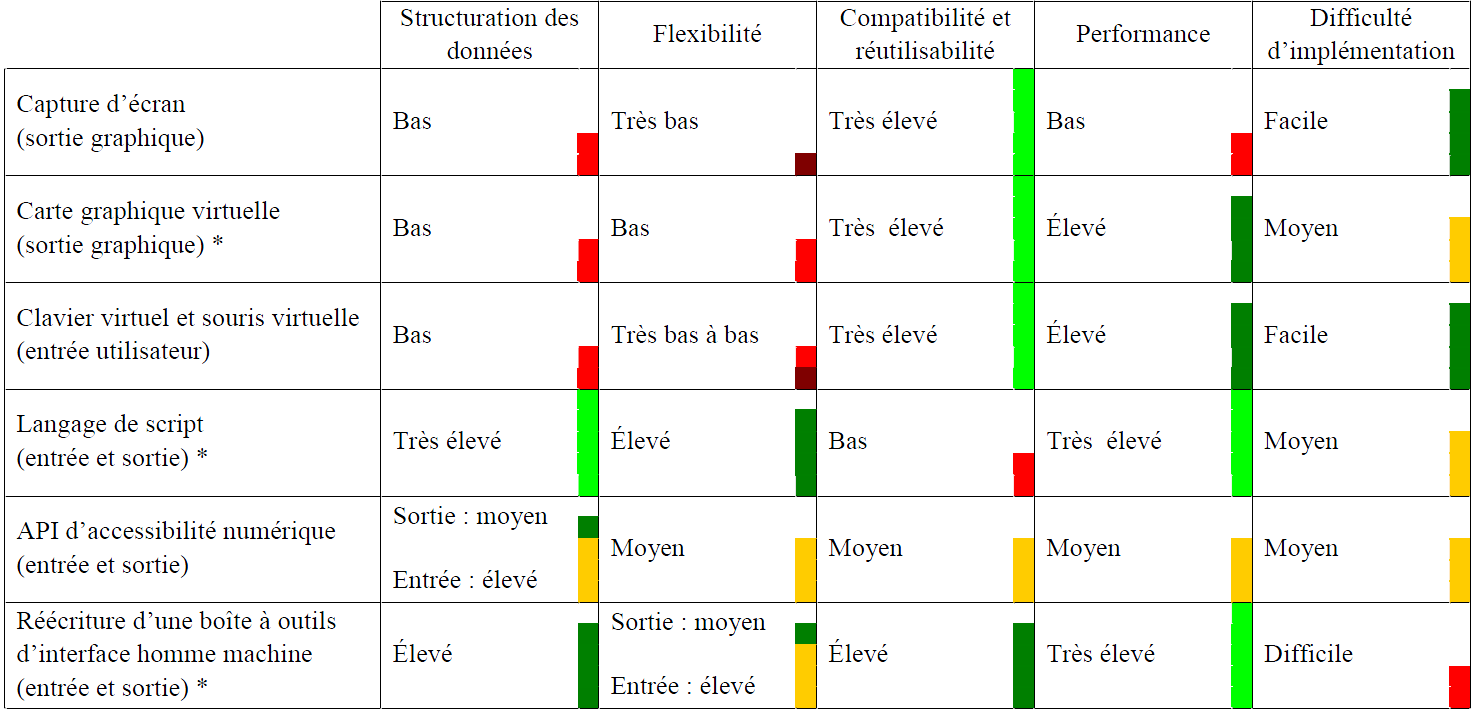
\includegraphics[angle=270,scale=0.55]{chap3/img-10}
%\caption{�valuation des technologies de r�utilisation des applications
%existantes sur les tables interactives}
%\label{fig:chap3:4}
%
%
%
%\end{center}
%
%\end{figure}

%\subsubsection{R��criture d'une bo�te � outils d'interface homme machine}
%\label{sec:chap3:1:2:1} 
consiste � utiliser la bo�te � outils de la table interactive � la place de celle du desktop. Le remplacement se fait en interceptant tous les appels de fonction de l'application vers les objets de la bo�te � outils d'IHM de d�part et en les redirigeant vers les �l�ments de la bo�te � outils de la table interactive. L'avantage de cette approche est d'utiliser des composants graphiques respectant les guidelines de la table interactive sans une nouvelle conception de l'application de d�part. Cette solution peut �tre impl�ment�e en utilisant les wrappers~\cite{Bartolomei2010} par exemple, le wrapper du listing~\ref{DescriptiveLabel} permet de r��crire un \textit{JComboBox}  en DSJComboBox. 
Cette approche ne permet pas le respect de l'ensemble des guidelines car la structure et le layout de l'UI par exemple n'est pas modifi�e pendant le portage. Elle permet de choisir les composants graphiques qui ont des interactions ou des styles conformes � la table interactive. 
%Cette solution couteuse en temps pour sa mise en place est sp�cifique pour les bo�tes � outils mais r�utilisable pour les applications d'une bo�te � outils.


%\definecolor{javared}{rgb}{0.6,0,0} % for strings
%\definecolor{javagreen}{rgb}{0.25,0.5,0.35} % comments
%\definecolor{javapurple}{rgb}{0.5,0,0.35} % keywords
%\definecolor{javadocblue}{rgb}{0.25,0.35,0.75} % javadoc
%
%\lstset{language=Java, basicstyle=\ttfamily,
%keywordstyle=\color{javapurple}\bfseries, stringstyle=\color{javared},
%commentstyle=\color{javagreen},
%morecomment=[s][\color{javadocblue}]{/**}{*/},numbers=left,
%numberstyle=\tiny\color{black}, stepnumber=2, numbersep=10pt, tabsize=4,
%showspaces=false,showstringspaces=false, caption=Exemple de wrapper,
%label=DescriptiveLabel}
%\lstinputlisting{chap3/listing.java}



\subsubsection{R�sum�}

%dans~\cite{Besacier2010} consid�re les guidelines pour la conception des UI collaboratives (cf.section~\ref{sec:chap2:3:3}) et en prenant en compte la m�taphore du papier~\cite{Besacier2007}.


%\fbox{\parbox{0.9\textwidth}{ La mise en \oe{}vre de cette solution induit la probl�matique de la description des \textbf{�quivalences entre les �l�ments des biblioth�ques graphiques} sources et cibles tout en pr�servant la nature des interactions en entr�e et en sortie.}}

\begin{table}[h]

\begin{tabularx}{15cm}{|Y|Y|Y|Y|}
\hline  \textbf{Approches}& \textbf{�quivalences} & \textbf{Mod�lisations} & \textbf{Guidelines} \\ 
\hline \textbf{Capture d'�cran }& Aucune �quivalence & Aucune mod�lisation & Aucune prise en compte \\ 
\hline \textbf{Carte graphique virtuelle }
						& Aucune �quivalence & Aucune mod�lisation  &  Aucune prise en compte\\ 
\hline \textbf{�mulation du clavier et de la souris} & �quivalences entre les dispositifs d'interactions en entr�e des plateformes source et cible d�finies manuellement 
						& Aucune mod�lisation  & Aucune prise en compte \\ 
\hline  \textbf{Langage de script}&
						 �quivalence manuelle des dispositifs d'interactions 
						 & Mod�lisation des donn�es, approche non r�utilisable &  Prise en compte des guidelines\\ 
\hline \textbf{API d'accessibilit� num�rique }& Manuelles &  Mod�lisation de la structure &  Prise en compte des guidelines \\ 
\hline \textbf{R��criture d'une boite � outils}  & Manuelles & Aucune & Prise en compte partielle \\ 
\hline 
\end{tabularx} 
\caption{Synth�se des approches de portage d'UI sur tables interactives}
\label{tab:chap3:4}
\end{table}
Il existe plusieurs solutions de portage des applications existantes sur les tables interactives. Les technologies pr�sent�es ci-dessus permettent la migration � l'ex�cution des applications sources. Ces approches sont limit�es car elles sont faiblement r�utilisables avec d'autres applications ou d'autres bo�tes � outils. 


Le tableau~\ref{tab:chap3:4} pr�sente une synth�se de ces technologies en prenant en compte les crit�res d'�quivalences entre les �l�ments de la plateforme, les mod�les utilis�s et la prise en compte des guidelines. L'on que remarque les �quivalences entre les dispositifs d'interactions sont d�crites manuellement pendant la mise en \oe{}uvre de la solution. Et toutes ces approches n'utilisent une mod�lisation des interactions et seulement deux approches mod�lisent la structure de l'UI. Les prises en compte des guidelines d�pendent du l'utilisation ou non de la bo�te � outils cible. En effet le langage de script, les API d'accessibilit� et la r��criture d'une bo�te � outils permettent d'utiliser  les �l�ments de la bo�te � outils cible. Cependant dans le cas de la r��criture d'une bo�te � outils, la prise en compte est partielle car la structure et le layout de l'UI de d�part ne sont pas modifi�s pendant le portage.


\section{Approches de migration bas�es sur les mod�les de l'UI }
\label{sec:chap3:3}

Cette section pr�sente des approches de migration bas�es sur des mod�les pour �tre ind�pendantes des applications et des plateformes. En effet les solutions de portage d'UI sur une table interactive pr�sent�es � la section~\ref{sec:chap3:1:2} utilisent des mod�les de donn�es et de structure de l'UI de d�part pour g�n�rer l'UI cible. Ces mod�les comportent des informations s�mantiques qui incluent pour chaque composant son nom, son r�le (bouton menu, case � cocher etc.), sa position sur l'�cran et dans la hi�rarchie en terme de contenant et de contenu. Cependant ces informations sont exploit�es par des m�canismes non r�utilisables et sp�cifiques � des applications car ces m�canismes sont constitu�s de scripts sp�cifiques � une fonctionnalit� d'une UI. 

Dans cette section nous �tudions les approches de migration qui se basent sur des mod�les qui d�crivent les diff�rents aspects de l'UI. D'abord l'approche MORPH\textit{ (Model Oriented Reengineering Process for HCI)}~\cite{Moore1997} qui mod�lise la structure et les interactions et qui d�crit des m�canismes de transformations de ces mod�les. Ensuite les approches bas�es sur les services de migration qui mod�lisent la structure, le layout, les interactions et le comportement des UI � migrer.


\subsection{Migration avec MORPH}

\label{sec:chap3:3:1}

MORPH~\cite{Moore1997} est une solution de migration d'une UI textuelle vers une UI graphique en se
basant sur des mod�les abstraits d'UI et un support pour les transformations
vers de nouvelles impl�mentations graphiques. Le processus de migration avec
MORPH implique une reconception de l'UI textuelle en UI graphique car les UI
graphiques de type WIMP~\cite{VanDam1997} supportent les dispositifs
d'interactions de manipulations directes comme une souris. Cette nouvelle
conception est aussi un \textbf{changement de modalit�s d'interactions} et
l'utilisation d'une bo�te � outils graphique. Nous �tudions cette approche de
migration car comme la migration d'UI vers des tables interactives, les
modalit�s d'interactions des plateformes d'arriv�e sont diff�rentes des
plateformes de d�part avec des nouveaux dispositifs d'interactions.

\subsubsection{Processus de migration}

\label{sec:chap3:3:1:1}

Il est repr�sent� par l'ensemble des m�canismes qui permettent l'extraction du
mod�le de l'UI, sa transformation et enfin sa g�n�ration pour la plateforme
cible. Les mod�les abstraits sont utilis�s pour la repr�sentation de  l'UI.

MORPH d�crit un processus  de migration en trois
�tapes : la d�tection, la repr�sentation et la transformation (cf. figure~\ref{fig:chap3:5}). 

\begin{itemize}

\item La \textbf{d�tection} est une activit� de reverse engineering qui consiste � analyser le code source de l'application � migrer dans le but d'identifier les mod�les de structure et d'interactions. 

\item La \textbf{g�n�ration} est l'op�ration inverse de la d�tection qui consiste � produire le code source de l'application migr�e � partir de mod�les abstraits transform�s.

\item La \textbf{repr�sentation} de l'UI de d�part est un ensemble de mod�les abstraits issu de la phase de d�tection. La \textbf{transformation} consiste � manipuler\footnote{Elle consiste � modifier les aspects visuels de l'UI � travers les mod�les  }, augmenter\footnote{Elle consiste � ajouter des composants graphiques ou des fonctionnalit�s � l'UI de d�part}, restructurer\footnote{Elle consiste a modifier les types de donn�es ou la structure hi�rarchique de l'UI} les mod�les abstraits de l'UI source pour �tre utilisables dans l'environnement
cible. 

\end{itemize}
	
\begin{figure}[h]

\begin{center}

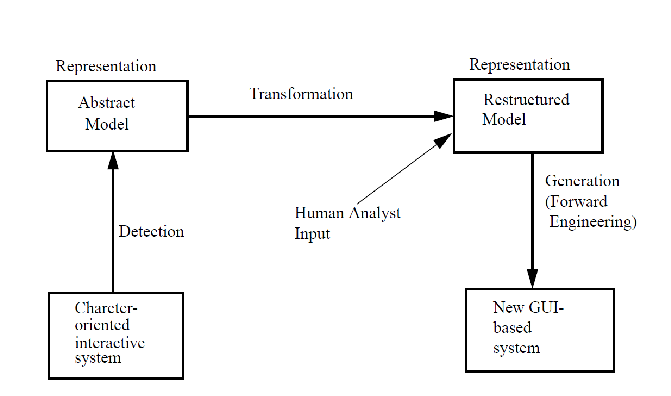
\includegraphics[ scale=1]{chap3/img-5}

\caption{Processus de migration avec MORPH}

\label{fig:chap3:5}

\end{center}

\end{figure}

\subsubsection{Les mod�les abstraits d'UI} 

\label{sec:chap3:3:1:2}

Ce sont des �l�ments cl�s du processus MORPH car ils repr�sentent les diff�rents
aspects (layout, activit�s, etc.)
de l'UI � migrer. Les mod�les sont d�crits suivant deux niveaux
d'abstractions:
\begin{itemize}
\item  le  niveau des \textbf{t�ches d'interactions} qui regroupe quatre interactions de base d'une UI ~\cite{Foley1990} qui sont : -la s�lection dans une liste, -la quantification ou la saisie d'une donn�e num�rique, -l'indication de la position\footnote{Sur une UI textuelle la position est exprim�e en termes de ligne et de colonne pour positionner le curseur du clavier par exemple} d'un �l�ment sur l'�cran et -la saisie d'une donn�e textuelle. Ces t�ches d'interactions sont identifi�es pour la migration d'UI textuelle vers une UI graphique. 
\item et le niveau d'\textbf{objet d'interactions abstraites} qui repr�sente les �l�ments abstraits ind�pendants d'une biblioth�que graphique (tel que Button, List, Menu, etc.), ce mod�le est sp�cifique aux UI graphiques.
\end{itemize}

Dans le cadre de la migration, les t�ches d'interactions permettent de d�crire les interactions des objets d'interactions abstraits ind�pendamment du dispositif d'interactions de d�part (clavier). \\


\fbox{\parbox{0.9\textwidth}{Les t�ches d'interactions constituent un \textbf{mod�le d'interactions abstraites} pour la migration d'une UI textuelle vers une UI graphique. }}\\  


Les objets d'interactions abstraits sont raffin�es � partir des attributs les diff�rentes t�ches d'interactions et en se basant sur le langage de repr�sentation des connaissances CLASSIC~\cite{Resnick1995}. 

\paragraph{Extraction des mod�les abstraits\\}
Les t�ches d'interactions et les objets d'interactions abstraites sont identifi�s � partir d'UI textuelles en se basant sur l'architecture de l'application � migrer et sur des \textbf{r�gles d'identifications}~\cite{Moore1996,Ratiu2008}. Pour identifier les t�ches d'interactions Moore et al.~\cite{Moore1996} d�crivent les r�gles d'identifications sous la forme: \[ Si\ \mathbf{Condition}\ est\ vraie;\ Alors\ identifier\ une\ \mathbf{T\hat{a}che\ d'interactions} \] o� $\mathbf{Condition}$ correspond � une situation d'une instance d'UI qui repr�sente une \textbf{T�che d'interactions} du mod�le abstrait. Cette forme de r�gle n�cessite que l'ensemble des situation soit identifi�es par un mapping entre la bo�te � outils de l'UI source et les interactions abstraites. 

Il existe d'autres approches pour extraire un mod�le � partir d'une UI existante, par exemple Ratiu et al.~\cite{Ratiu2008} proposent une ontologie pour analyser et comprendre des API sp�cifiques � un domaine comme les biblioth�ques graphiques. Le principe de l'approche consiste d'abord � construire une ontologie capable de repr�senter les concepts d'une biblioth�que graphique que l'on souhaite utiliser pour la migration; dans notre cas ce sont la structure et les interactions abstraites d'une UI. Dans notre cas l'ontologie d�crirait les liens de contenance entre les composants graphiques, les donn�es et les t�ches interactions en entr�e (s�lection, quantification, position, �dition). 

Ensuite, � partir d'une UI d�crite � l'aide des instances des �l�ments d'une biblioth�que graphique, l'on extrait gr�ce � l'ontologie les objets d'interactions abstraites. Cette extraction est possible gr�ce � un algorithme d'extraction d�crit dans~\cite{Ratiu2008}. Les objets d'interactions abstraites de l'UI source sont utilis�s comme pivot pour d�crire l'UI cible. 

Cette approche d'extraction pr�sente un avantage par rapport aux r�gles d'identifications de~\cite{Moore1996} car elle ne s'appuie pas sur des situations d�crivant des cas possibles dans une UI mais elle se base sur les types des �l�ments utilis�s pour d�crire l'UI et elle est plus g�n�rique. Cependant le choix de l'ontologie doit �tre exhaustive pour une API et pour les concepts qui sont repr�sent�s.


%En consid�rant une application qui respecte une architecture ARCH et en analysant statiquement les codes sources du composant de pr�sentation de cette application, les r�gles d'identification des objets d'interactions abstraites et des t�ches d'interactions permettent de distinguer les menus des listes de s�lection.


\paragraph{M�canismes de transformations et de g�n�ration de  l'UI\\ }

Une fois l'UI source d�crite par les t�ches d'interactions et ensuite raffin�e en objets d'interactions abtraites,  la repr�sentation abstraite de l'UI de d�part est transform�e en modifiant manuellement le mod�le d'UI. 

Le \textbf{transformation} consiste d'une part � remplacer des objets d'interactions de l'UI source. Par exemple une t�che de s�lections dans une liste  qui est raffin�e en une liste � choix unique peut �tre remplac�e par un menu si le nombre d'�l�ments est inf�rieur � 10. 

D'autre part cette phase fait intervenir un utilisateur humain pour d�finir la position, la taille ou pour modifier l'UI. Le concepteur intervient manuellement sur les mod�les d'UI apr�s la transformation dans le but de placer les �l�ments de l'UI. En effet, l'UI textuelle de d�part n'est pas structur�e comme une UI graphique et les mod�les de t�ches d'interactions et d'objets abstraits d'interactions ne permettent pas de d�crire le layout par exemple.


La s�lection des �l�ments de la biblioth�que graphique cible se fait en recherchant dans une biblioth�que graphique d�crite par une ontologie des �l�ments qui correspondent le plus � un objet abstrait du mod�le restructur�. 


\fbox{\parbox{0.9\textwidth}{
Le mapping entre objets abstraits et les �l�ments d'une biblioth�que graphique est fait \textbf{dynamiquement en se basant sur les ontologies}. En effet les correspondances entre les objets abstraits et les �l�ments de la biblioth�que graphique ne sont pas d�finies manuellement et de mani�re exhaustives � la conception de la solution, mais elles sont �tablies en se basant sur les attributs de chaque �l�ments.}}


Les m�canismes de transformations et g�n�rations utilis�s par MORPH sont bas�s aussi sur des ontologies. Dans le cadre de la transformation par exemple il est possible d'introduire des guidelines dans la base de connaissances, en pr�f�rant remplacer une liste en menu si elle contient moins de 10 �l�ments par exemple.


\fbox{\parbox{0.9\textwidth}{La transformation utilis�e par MORPH permet d'inclure les principes de conception d'UI pour la plateforme cible dans la base de connaissances~\cite{Moore1997}.}}

%faite sur les attribut des t�ches d'interactions. elle permet d'�tablir des r�gles d'�quivalences entre les mod�les abstraits sources et cibles en se basant sur les r�les. Par exemple un AWT-Choice est �quivalent � un  MORPH-BASIC-MENU au nombre d'�tat pr�s suivant le tableau~\ref{tab:chap3:2} et ceci ind�pendamment des types des t�ches d'interactions.
%Le mod�le abstrait d�crit � la fois les interactions de l'utilisateur (la s�lection, l'�dition, etc.) et les composants graphiques (bouton, liste de s�lection, menu etc.) ind�pendamment des biblioth�ques graphiques.

%\begin{table}[h]
%
%\vspace{3pt} \noindent
%
%\begin{tabular}{|p{113pt}|p{85pt}|p{180pt}|}
%
%\hline
%
%\parbox{113pt}{\raggedright 
%
%\textbf{{\footnotesize Composants Graphiques}}
%
%} & \parbox{85pt}{\raggedright 
%
%\textbf{{\footnotesize Objets d'Interactions}}
%
%} & \parbox{180pt}{\raggedright 
%
%\textbf{{\footnotesize R\^{o}les} }
%
%} \\
%
%\hline
%
%\parbox{113pt}{\raggedright 
%
%{\footnotesize MORPH-RADIO-BUTTON}
%
%} & \parbox{85pt}{\raggedright 
%
%{\footnotesize SELECTION-OBJECT}
%
%} & \parbox{180pt}{\raggedright 
%
%{\footnotesize -action= Visible-State-Change}
%
%
%
%{\footnotesize -number-of-states=2}
%
%
%
%{\footnotesize -variability = fixed}
%
%
%
%{\footnotesize -grouping= grouped}
%
%} \\
%
%\hline
%
%\parbox{113pt}{\raggedright 
%
%{\footnotesize MORPH-BASIC-MENU}
%
%} & \parbox{85pt}{\raggedright 
%
%{\footnotesize SELECTION-OBJECT}
%
%} & \parbox{180pt}{\raggedright 
%
%{\footnotesize -action= Procedural-Action}
%
%
%
%{\footnotesize -number-of-states=(min=2, max=10)}
%
%
%
%{\footnotesize -variability = fixed}
%
%
%
%{\footnotesize -grouping= not-grouped}
%
%} \\
%
%\hline
%
%\parbox{113pt}{\raggedright 
%
%{\footnotesize AWT-Choice}
%
%} & \parbox{85pt}{\raggedright 
%
%{\footnotesize INTERACTION-OBJECT}
%
%} & \parbox{180pt}{\raggedright 
%
%{\footnotesize -action=Procedural-Action}
%
%
%
%{\footnotesize -number-of-states=(min=2, max=15)}
%
%
%
%{\footnotesize -variability = fixed}
%
%
%
%{\footnotesize -grouping= not-grouped}
%
%} \\
%
%\hline
%
%\end{tabular}
%
%\caption{Composant graphique et r�les}
%
%\label{tab:chap3:2}
%
%\end{table}

%Dans le cas de la migration d'UI vers une table interactive, la description des
%mod�les d'interactions et des composants graphiques ind�pendamment des �l�ments
%de la plateforme facilite leur mise en correspondances.





\subsubsection{Comment adapter MORPH pour la migration d'UI vers les tables interactives?}

La r�ponse � cette question passe d'abord par l'ajout de la biblioth�que graphique de la table interactive � la base de connaissances pour permettre l'extraction et la g�n�ration de l'UI finale. Ensuite, il faut d�crire les mod�les abstraits.  Par exemple, nous utilisons les mod�les abstraits de l'approche MORPH pour repr�senter les interactions des �l�ments graphiques d'un art�fact de l'UI
CBA cf. figure~\ref{fig:chap2:2}: 
\begin{itemize}
	\item le menu principal a une t�che d'interactions de type SELECTION-OBJET avec les r�les (action = \textit{Procedural-Action}, number-of-states = (2..10), variability = \textit{fixed}, grouping= \textit{not-grouped})
	\item la liste d�roulante (\textit{ComboBox}) a une t�che d'interactions de type SELECTION-OBJET avec les r�les (action= \textit{Procedural-Action}, number-of-states = (2..10), variability = \textit{fixed}, grouping = \textit{not-grouped})
	\item la liste d'images a une t�che d'interactions de type SELECTION-OBJET avec les r�les (action = \textit{Procedural-Action},  number-of-states = (2..10), variability = \textit{fixed}, grouping = \textit{not-grouped})
\end{itemize}

Enfin, il faut mettre en place des r�gles de transformations des mod�les abstraits en prenant en compte les guidelines. Par exemple, la prise en compte de la guideline~\ref{guide:7} d'utilisation en 306� des �l�ments graphiques consiste � remplacer les composants graphiques contenant d'autres avec ceux qui ont ces interactions. Les mod�les abstraits doivent �tre capables de d�crire et de s�lectionner les composants graphiques conformes � une guideline.

%Cette transformation pose un probl�me de regroupement des �l�ments graphiques migr�s sur la table interactive. En effet sur l'exemple ci-dessous (cf figure~\ref{fig:chap3:14}), la liste d�roulante et la liste d'images par exemple doivent �tre regroup�s dans un m�me container car l'utilisation de ces deux composants se fait au m�me moment par un utilisateur.


%La r�utilisation de ce processus de migration dans le cadre de la migration vers une table interactive \textit{DiamondTouch} par exemple n�cessite  un mapping entre les objets d'interactions abstraites et chaque �l�ment de la biblioth�que graphique \textit{DiamondSpin} . 


%\begin{figure}[h]
%
%\begin{center}
%
%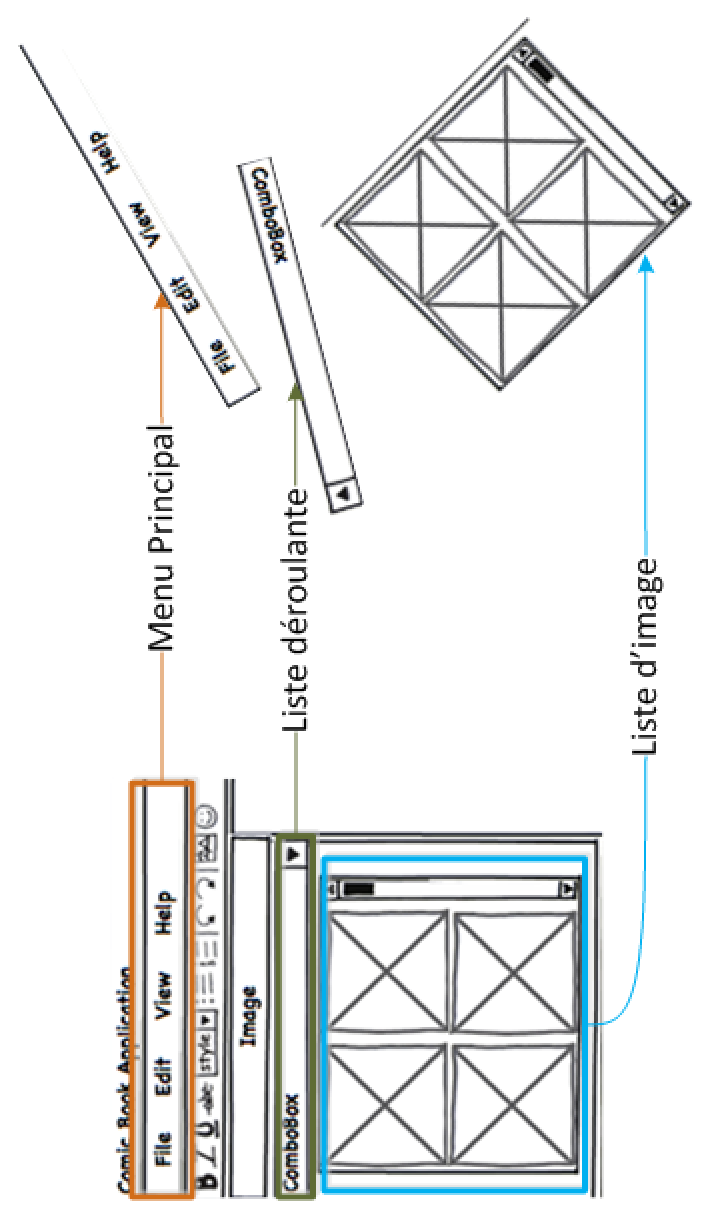
\includegraphics[angle=270, scale=.4]{chap3/img-15}
%
%\caption{Migration vers une table interactive avec MORPH}
%
%\label{fig:chap3:14}
%
%\end{center}
%
%\end{figure}



\subsubsection{R�sum�}
\label{sec:chap3:3:1:3}


Cette approche propose une solution de migration r�utilisable qui prend en compte une phase reverse engineering (\textbf{d�tection}), une phase de re engineering (\textbf{transformation}) et une phase de forward engineering (\textbf{g�n�ration}). Le tableau~\ref{tab:chap3:2} pr�sente l'approche MORPH suivant les caract�ristiques d'�quivalences des �l�ments des plateformes, de mod�lisation et de prise en compte des guidelines.


L'approche est bas�e sur des mod�les abstraits qui d�crivent la structure et les interactions (et les comportements) des UI � migrer. Le layout et le style des UI ne sont pas mod�lis�s par cette approche, leur migration est effectu� manuellement par un utilisateur humain. 
Cependant les mod�les abstraits propos�s par MORPH ne sont pas adapt�s pour �tre utilis�s pour une plateforme comme une table interactive.  Le mod�le de t�che d'interactions par exemple ne prend pas en compte les mouvements (rotation, d�placement, etc) des composants graphiques des tables interactives. Le mod�le de t�che d'interactions permet d'�tablir des �quivalences entre dispositifs d'interactions en se basant sur des t�ches de haut niveau d'abstraction et ind�pendantes des plateformes. Cependant ce mod�le n'est pas exhaustif.

En ce qui concerne les �quivalences entre les biblioth�ques graphiques par exemple, elles sont bas�es sur les mod�les de connaissances et elles sont �tablies dynamiquement.

\fbox{\parbox{0.9\textwidth}{
 Les �quivalences dynamiques entre les biblioth�ques graphiques permettent de s�lectionner les composants graphiques appropri�s pour chaque cas en fonction de leurs caract�ristiques d'utilisation. }}



Par ailleurs cette approche permet la prise en compte des guidelines � travers les transformations (remplacement des objets abstraits ou s�lection des composants graphiques sp�cifiques). Cependant l'identification des guidelines et leur prise en compte pendant la transformation sont � d�crire par le concepteur de la solution de migration sur une plateforme comme les tables interactives.

\begin{table}[h]
\begin{tabularx}{15cm}{|Y|Y|Y|Y|}
\hline  & \textbf{�quivalences} & \textbf{Mod�lisations} & \textbf{Prise en compte des guidelines}  \\ 
\hline \textbf{MORPH} & Dynamique des biblioth�ques graphiques  bas�es sur des mod�les de connaissances 
			& Mod�lisation des interactions abstraites,   Mod�lisation de la structure 
			& Prise en compte par les r�gles de transformations des mod�les abstraits \\ 
\hline 
\end{tabularx} 
\caption{R�capitulatif de MORPH}
\label{tab:chap3:2}
\end{table}



\subsection{Approches de migration automatiques d'UI}
\label{sec:chap3:3:2}
La solution MORPH ne mod�lise pas tous les aspects d'une UI, ce qui implique une intervention de l'utilisateur pour la migrations des aspects non g�r�s. Dans cette section nous pr�sentons les approches de migration r�utilisables pour diff�rentes plateformes en s'appuyant sur des mod�les abstraits d'UI et qui ne font pas appel � des processus manuels.

Ces solutions de migration d'UI sont g�n�riques et sont utilis�es par des services de migration des UI dans des contextes ubiquitaires comportant plusieurs types de plateformes. Les services de migration d'UI sont charg�s d'adapter une UI pendant son ex�cution\footnote{C'est une migration � la vol�e d'une UI d'une application o� l'�tat courant de l'UI est sauvegard� par des mod�les abstraits d'UI et adapt� sur une autre plateforme en permettant � l'utilisateur de continuer une t�che sans interruption~\cite{Calvary2002}} ou entre deux sessions de son utilisation\footnote{C'est une migration qui implique que l'utilisateur quitte l'application, sauvegarde son �tat et red�marre l'application sur la nouvelle plateforme~\cite{Calvary2002}}  pour une plateforme donn�e. Nous �tudions dans cette section les mod�les d'UI et les m�canismes de ces approches pour la migration d'UI vers une table interactive.

\subsubsection{Mod�les d'UI}
\label{sec:chap3:3:2:1}
Les mod�les abstraits permettent de d�crire les UI comportant en g�n�ral plusieurs niveaux d'abstraction dans l'objectif de d�crire les diff�rents aspects des UI. Le framework de r�f�rence CAMELEON (CRF)~\cite{Calvary2002} propose quatre niveaux d'abstraction pour d�crire les UI: le niveau des t�ches et concepts, le niveau interface abstraite (AUI), le niveau interface concr�te (CUI) et le niveau interface finale (FUI). 

\paragraph{Mod�le de t�ches et concepts} Ce mod�le exprime les t�ches  et les concepts d'UI dans un contexte pr�cis tel que d�fini par le concepteur. 
Ce mod�le exprime les interactions de l'UI avec les utilisateurs ou le syst�me, le comportement et les diff�rents �tats des composants graphiques. Dans le cadre de la migration des UI � la vol�e, le mod�le de t�ches permet de conserver l'�tat d'une UI en cours d'ex�cution par exemple. 

Dans notre cas, la migration ne se fait pas � l'ex�cution, mais elle se fait de mani�re statique et elle passe par une re conception de l'UI de d�part. Le mod�le de t�ches peut permettre d'exprimer les interactions entre les utilisateurs et l'UI ind�pendamment des modalit�s d'interactions.
\paragraph{Mod�le AUI} Ce mod�le permet de repr�senter les �l�ments d'une UI ind�pendamment des modalit�s d'interactions en exprimant leur fonctionnalit� essentielle. Ce mod�le concr�tise les �l�ments du domaine utilis� par le mod�le de t�ches, par exemple une t�che de saisie de donn�es correspond � un �l�ment de type Input dans le mod�le AUI (cf. figure~\ref{fig:chap3:2}). Les �l�ments du mod�le AUI permettent en g�n�ral d'exprimer les diff�rents types d'interactions tels que l'entr�e de donn�es (Input), l'affichage d'informations (Output), l'activation d'une commande (Command). Ce mod�le exprime aussi la structure d'une UI � travers les regroupements (Container) ou les types des donn�es. 

Dans notre cas, le mod�le d'AUI exprime les interactions de haut niveau entre UI et NF et ind�pendamment des dispositifs d'interactions. Cependant ce mod�le n'exprime pas les interactions sur les propri�t�s visuelles des composants graphiques (redimensionnement, d�placement, rotation, etc.). En effet le mod�le AUI est ind�pendant de toute modalit�, il peut �tre concr�tis� en UI graphique, vocale, multimodale, etc.

\paragraph{Mod�le CUI} Ce mod�le permet de d�crire une repr�sentation concr�te de l'UI suivant une modalit�. Dans le cadre des UI graphiques qui nous concernent par exemple, des composants graphiques sont choisies pour raffiner les �l�ments du mod�le AUI. Ce mod�le exprime la structure, le positionnement (layout) et m�me le style des �l�ments graphiques. Les composants graphiques de ce mod�le sont exprim�s dans un langage ind�pendant des biblioth�ques graphiques pour garantir leur r�utilisabilit�. 

Dans notre cas, le mod�le de CUI exprime des UI de modalit� graphique et l'on peut consid�rer la migration d'UI desktop vers une table interactive comme un changement de biblioth�que graphique qui n�cessite une adaptation des interactions, de la structure, du layout et du style de l'UI de d�part.

Il existe plusieurs impl�mentations pour chacun de ces niveaux de mod�le. Patern� \textit{et al}.~\cite{Paterno'2009} proposent le langage MARIA XML qui d�crit les UI aux niveaux (AUI et CUI) et USIXML (User Interface eXtensible Markup Language)~\cite{Vanderdonckt2004} d�crit aussi des mod�les de CUI, AUI.


%Le lien entre ces diff�rents niveaux d'abstraction �tant assur� par un mod�le de mapping, le processus de d�veloppement consiste en un raffinement successif du niveau le plus abstrait pour atteindre une plateforme pr�cise. En effet l'application est sp�cifi�e d'abord sous forme de t�che et de concept qui seront raffin�s en AUI, ensuite en CUI et enfin en FUI  (cf. figure~\ref{fig:chap3:2}).

%TODO:
%Le mod�le CUI d�crit la structure d'une UI: Donn�es, le regoupement, la cardinalit� de l'UI
%Ce mod�le dans certain cas d�crit le layout de l'UI aussi
\begin{figure}[ht]

\begin{center}

 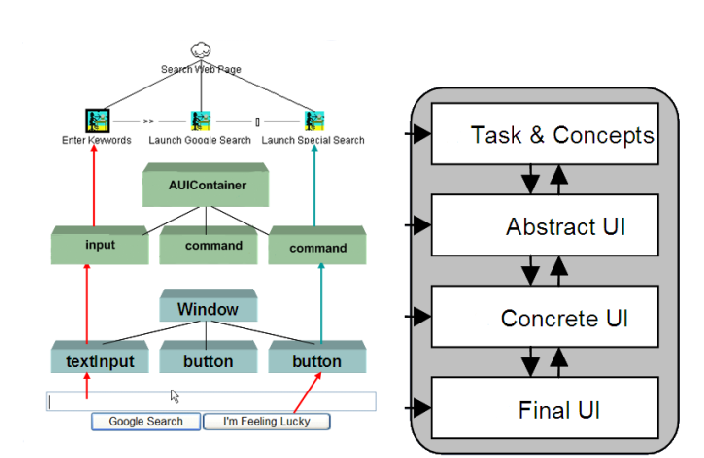
\includegraphics[scale=.8]{chap3/img-7} 

 \caption{Exemple de transformation USIXML}

 \label{fig:chap3:2}

\end{center}

\end{figure}


%\fbox{\parbox{0.9\textwidth}{Les mod�les des niveaux d'abstractions de t�ches,  d'AUI et de CUI sont utilis�s par les m�canismes de migrations pour transformer l'UI de d�part � la plateforme cible. }}

Les diff�rents mod�les du CRF permettent de concevoir des UI multi plateformes, dans une approche de conception top down qui consiste � partir du mod�le le plus abstrait (mod�le de t�ches et concepts), le concepteur g�n�re les UI par raffinements successifs des mod�les du CRF. Dans le cadre de la migration d'UI, ces mod�les sont utilis�s soit par des m�canismes de g�n�ration des UI finales pour la nouvelle plateforme � partir des mod�les abstraits~\cite{Macias2006}, soit par reverse engineering de l'UI existante~\cite{Paterno2010}.

\subsubsection{M�canismes de migration d'UI top down}
\label{sec:chap3:3:2:3}
Nous appelons les m�canismes de migration d'UI bas�s sur le raffinement des mod�les abtraits du CRF en migration d'UI top down. En effet, les concepteurs g�n�rent par exemple le mod�le CUI sp�cifique � chaque plateforme � partir des mod�les AUI et t�ches. Cette approche permet de migrer les �tats d'UI  � l'ex�cution, MigriXML~\cite{Macias2006} par exemple d�finie gr�ce � ces m�canismes un environnement virtuel comprenant diff�rentes plateformes (desktops avec diff�rentes tailles d'�cran, smartphones, etc.)

La g�n�ration des mod�les les moins abstraits dans cette approche est effectu�e � la conception. L'approche permet d'�tendre une application � d'autres plateformes en r�utilisant les mod�les de t�ches et d'AUI dans le cas d'une nouvelle plateforme ayant des modalit�s diff�rentes de la plateforme de d�part. 
Pour la migration d'une application existante par ces m�canismes, il est indispensable d'avoir les mod�les du CRF associ�s. Cette contrainte exclue toutes les UI des applications qui ne sont pas con�ues suivant le CRF.

%Ces m�canismes ont pour objectif de faciliter le changement de modalit�s d'interactions de l'UI de d�part. Kong et al.~\cite{Kong1999a} proposent � cet effet un mod�le de t�ches\footnote{Ce mod�le de t�ches est utilis� par un processus de migration g�n�rique d'une UI textuelle vers une UI graphique.} bas� sur les \textit{actions des utilisateurs}, sur les \textit{�crans }et les transitions entre les diff�rents �crans. Ce mod�le identifie trois types d'actions:
%
%\begin{itemize}
% \item les actions d'entr�e de donn�e (\textit{tell}), 
% \item les actions d'affichage d'informations � un m�me endroit de l'�cran (\textit{ask-standard}\footnote{Dans le cadre d'une UI textuelle, certaines zones de l'�cran peuvent �tre utilis�es pour pr�senter des informations de progression par exemple. }) 
% \item et les actions d'affichage d'informations � diff�rents endroits de l'�cran(\textit{task-select}). 
%\end{itemize}
%
%Les trois types d'actions permettent d'identifier les diff�rentes informations �chang�es entre l'application et l'utilisateur. Les activit�s permettent de repr�senter le actions possibles de l'utilisateur � partir de l'UI textuelle dans le but de d�duire le mod�le d'interface abstrait. Par exemple les actions de types \textit{tell} qui manipulent les dates sont repr�sent�es par des objets graphiques qui peuvent �tre des calendriers.
%
%
%Dans le cadre de la migration d'une UI desktop vers une table interactive, le mod�le de t�ches peut permettre la prise en compte de la guideline  de ``couplage t�ches et utilisateurs'' (G\ref{guide:5}) et se fait en identifiant et en supprimant les activit�s bloquantes pour les autres utilisateurs telles que l'affichage d'une bo�te de dialogue par exemple.
%
%
%Par ailleurs, les trois types d'actions identifi�es ci-dessus ne permettent pas de repr�senter toutes les activit�s possibles sur une UI desktop. En effet, les interactions en entr�e par exemple peuvent �tre des saisies de donn�es ou des commandes (d�placement, redimensionnement ou activation) avec ou sans param�tre.\\
%
%\fbox{\parbox{0.9\textwidth}{
%Les mod�les d'interactions abstraites permettant de repr�senter l'ensemble des activit�s possibles des plateformes sources et cibles et peuvent �tre utilis�s pour repr�senter le mod�le de t�ches.}}

\subsubsection{M�canismes de migration d'UI bottom up}
\label{sec:chap3:3:2:4}
Ces m�canismes permettent la migration d'UI en utilisant les mod�les du CRF et en les abstrayant � partir d'UI existantes. 
%Les m�canismes de migration bas�s sur les mod�les AUI et CUI sont utilis�s par plusieurs solutions de migrations~\cite{Masso2006,Wong}. 
Patern� \textit{et al}.~\cite{Paterno2010} proposent un service d'adaptation d'une page web � un t�l�phone portable~\ref{fig:chap3:1}   bas� sur le reverse engineering et l'adaptation d'une UI existante. Ce service abstrait les pages HTML dans les mod�les CUI et AUI du langage MARIA XML et transforme les mod�les obtenus en fonction de ces principes:
\begin{itemize}

\item adapter les tableaux en les d�coupant en plusieurs tableaux pour ceux comportant plusieurs colonnes ou en r�duisant les donn�es qu'ils contiennent (si une cellule d'un tableau contient un nombre maximum de mots alors on cr�e un lien ``\textit{d�tail...}'' pour afficher les contenus en trop)

\item transformer les textes longs en liens ``\textit{d�tail...}'' comme pour les contenus des tableaux

\item transformer les images en les redimensionnant

\item convertir les listes en menu drop down par exemple

\item adapter la taille et la disposition des composants graphiques en les redimenssionnant et en adoptant un layout vertical par exemple

\end{itemize}

Le concepteur d�finie des m�canismes de transformations~\cite{Limbourg} pour appliquer ces principes sur les mod�les de CUI et d'AUI. Dans ce cas, la migration ne change pas de biblioth�que graphique car l'UI reste toujours en HTML. Cependant le layout, la taille des composants graphiques, les donn�es et le type de certains composants graphiques sont transform�s et remplac�s pendant la migration. Les transformations des instances des mod�les AUI et CUI de l'UI de d�part sont horizontales car elle g�n�rent d'autres instances de ces mod�les pour la plateforme d'arriv�e.

L'avantage de cette approche  est que seuls les mod�les indispensables pour la migration sont abstraits � partir de l'UI de d�part. En effet, pour adaptation du layout par exemple, le mod�le de t�che n'est pas indispensable. Dans le cadre de la migration d'UI vers les tables interactives qui implique un changement de dispositifs d'interactions, il est indispensable d'exprimer les interactions de mani�re abstraite par les mod�les du CRF (T�ches et AUI). Cependant les mod�les de t�ches et AUI du CRF n'expriment pas toutes les interactions des tables interactives (cf. section~\ref{sec:chap3:3:2:1}). Ces m�canismes bas�es sur le reverse engineering n�cessitent aussi que les applications respectent des architectures pr�nant la s�paration entre UI et NF (telles que MVC ou ARCH).

 \begin{figure}[h]

 \begin{center}

 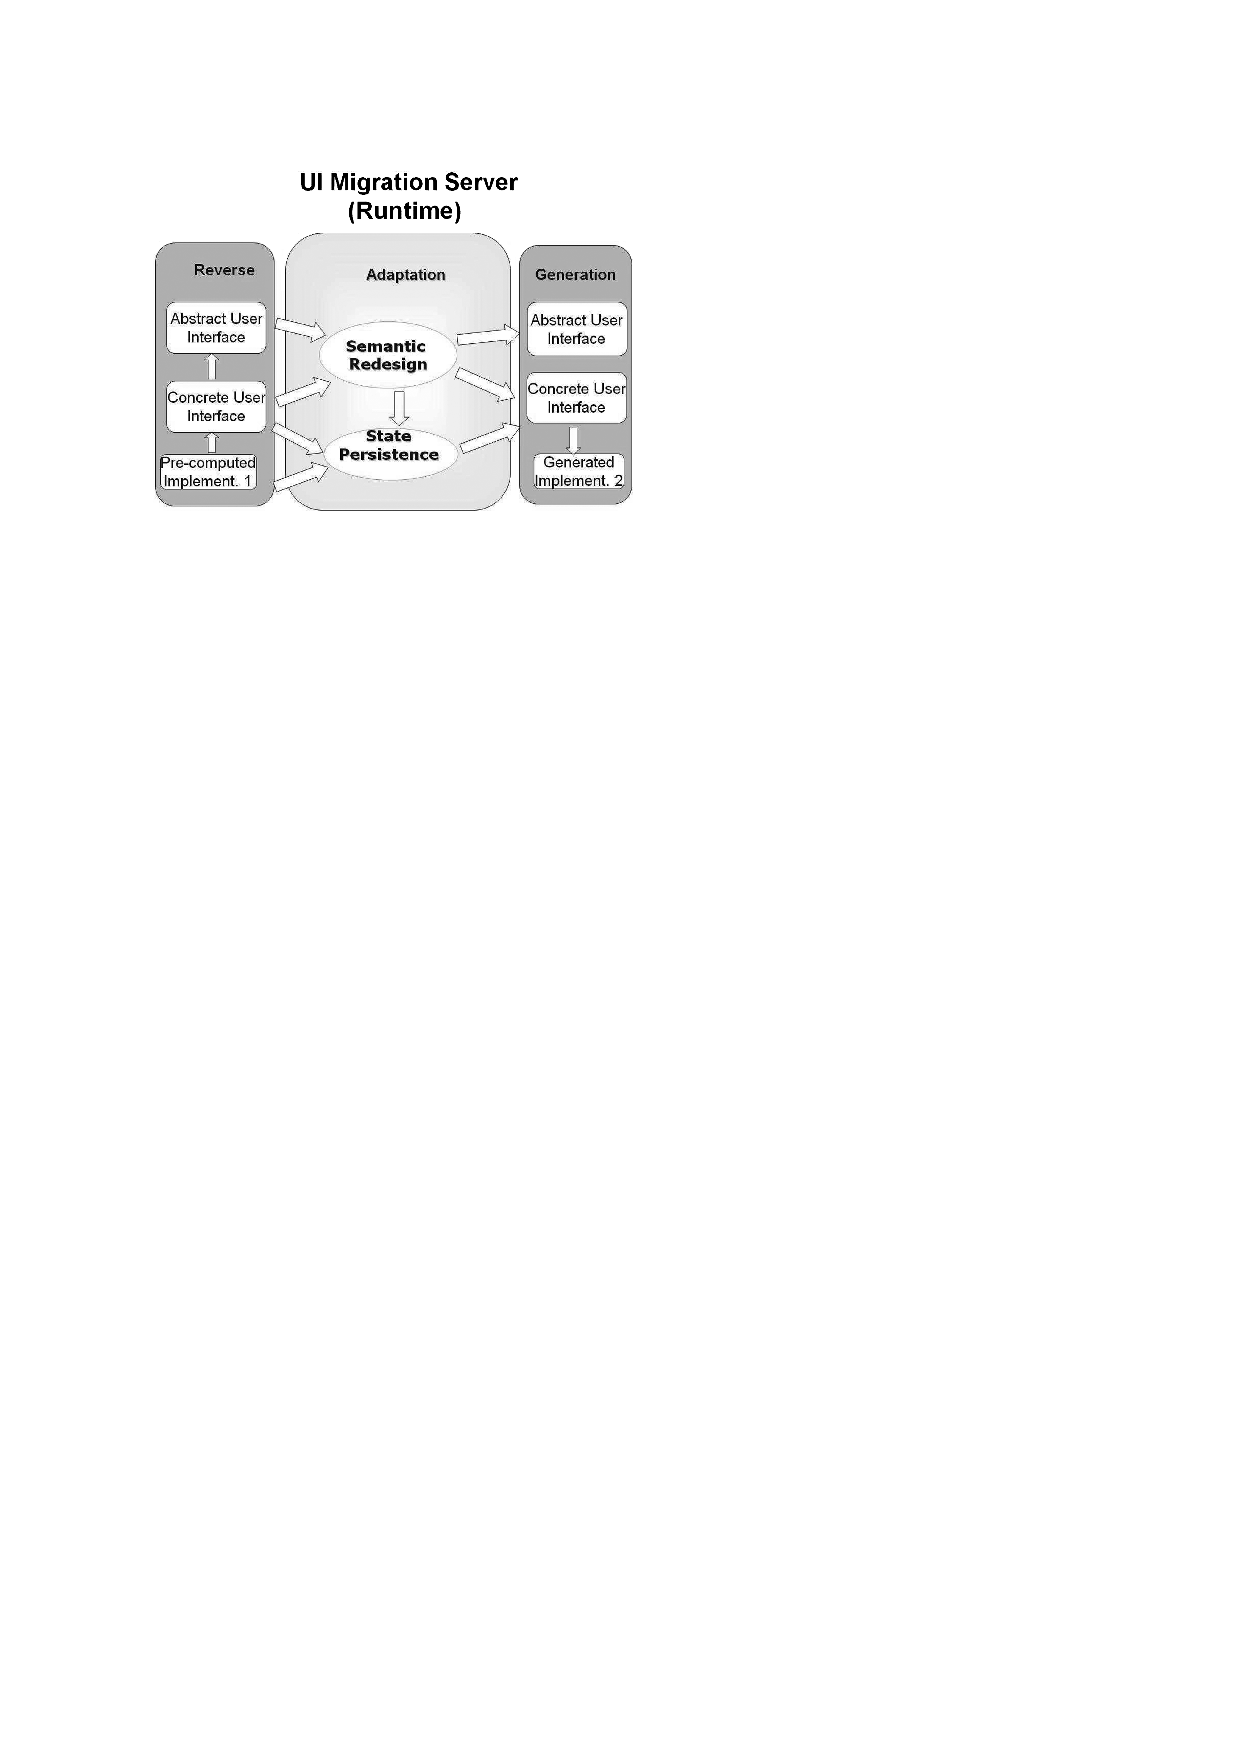
\includegraphics[scale=1]{chap3/img-6} 

 \caption{Service de migration d'UI}

 \label{fig:chap3:1}

 \end{center}

 \end{figure}


\subsubsection{Service de migration d'UI desktop vers les tables interactives}
%L'utilisation d'un serveur de migration d'UI pour les tables interactives
%implique la possibilit� d'extraire les mod�les abstraits des applications �
%migrer et formalisation des r�gles de transformation des mod�les de
%l'application de d�part pour la plateforme d'arriv�e.\\

Dans cette section nous �tudions les adaptations n�cessaires dans le cas d'une r�utilisation du service de migration d'UI (cf. figure~\ref{fig:chap3:1}). Nous choisissons d'adapter cette solution car elle prend en compte des UI sources en retrouvant les mod�les abstraits n�cessaires. Nous consid�rons toujours  notre exemple fil rouge :l'application CBA (cf. section~\ref{sec:chap2:2:1}) � migrer sur une table interactive (Microsoft PixelSense). 
Une adaptation du service de migration d'UI n�cessite:
\begin{itemize}
	\item  une table d'�quivalences (tableau~\ref{tab:chap3:1}) entre les �l�ments du langage MARIA XML, XAML et l'API Java Swing pour abstraire et concr�tiser l'UI de d�part
	\item une formalisation des guidelines sur les �l�ments du langage MARIA XML.
\end{itemize}
    
   


\begin{table}[h]
\caption{Table d'�quivalences}
\label{tab:chap3:1}
\begin{center}
\begin{tabular}{|c|c|c|}

\hline \textbf{MARIA XML}&	\textbf{Java Swing}&	\textbf{XAML Surface}\\ 

\hline Activator&	JButton&	Button\\ 

\hline Single choice&	JCombox&	ListBox\\ 

\hline Text Edit&	JTextField&	TextBox\\ 

\hline Object&	Image&	Image\\ 

\hline Grouping&	JPanel&	  {\footnotesize ScatterViewItem, Grid}\\
\hline 
\end{tabular} 

\end{center}
\end{table}

La table d'�quivalence permet de d�crire les correspondances entre les
biblioth�ques graphiques des plateformes sources et cibles. Le
tableau~\ref{tab:chap3:1} par exemple d�crit une correspondance entre Java Swing
et XAML en se basant sur le langage MARIA XML. Cette correspondance est statique
et doit �tre �tablie pour l'ensemble des composants graphiques d'une
biblioth�que graphique.

Par ailleurs, Silva \textit{et al.}~\cite{Silva2012} proposent plusieurs crit�res pour la
correspondance entre biblioth�ques graphiques bas�es sur les langages XML. Le
premier crit�re est le comportement des composants graphiques car il caract�rise
les actions utilisateurs ind�pendamment de la repr�sentation du composant
graphique. Les autres crit�res utilisables dans le cadre de la migration sont le
style des UI et les balises des �l�ments graphiques.

En consid�rant par ailleurs la guideline d'utilisation 360� (G\ref{guide:7}),
elle peut �tre traduite sur les �l�ments
du langage MARIA XML, qui par exemple  donne la r�gle suivante: tous les
\textit{Grouping} sont
transform�s en ScatterViewItem pour �tre conformes � la guideline d'utilisation
360�de l'UI.


%\begin{figure}[ht]

%\begin{center}
% 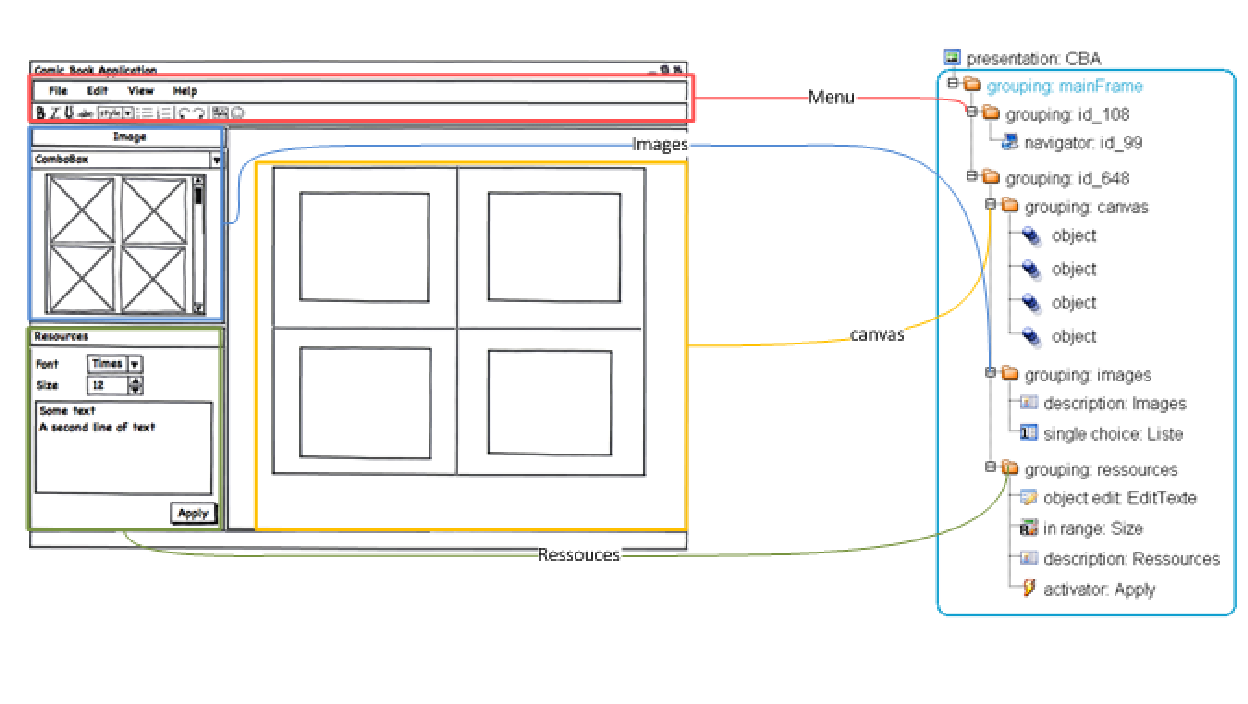
\includegraphics[scale=.5]{chap3/img-14} 
%  \caption{Processus de migration d'une UI Desktop vers un t�l�phone portable}
%  \label{fig:chap3:3}
 
%\end{center}

%\end{figure}

\subsubsection{R�sum�}
%Les serveurs de migration pr�sent�s dans cette section se basent sur des mod�les d'UI pour leur permettre de d�crire des m�canismes de migration g�n�riques. Le mod�le d�crivant les actions utilisateurs et les transitions des �crans propos�s par Kong et al.~\cite{Kong1999a} peut �tre consid�r� aussi comme un mod�le de t�che. Dans notre contexte de migration, ce mod�le permet de d�duire le AUI et permet aussi  la prise en compte de guidelines pour la table interactive.
Cette section pr�sente des m�canismes de migration d'UI bas�s sur les mod�les de CRF. Le mod�le de CUI graphique permet de d�crire la structure hi�rarchique, les donn�es et le positionnement d'une UI. Dans un m�canisme de migration d'UI vers la table interactive, le mod�le de CUI est transform� pour rendre l'UI de d�part conforme aux guidelines. 

Le mod�le d'AUI d�crit � la fois le regroupement des �l�ments abstraits d'UI et les interactions (en entr�e ou en sortie) entre l'utilisateur et le syst�me (NF). Les mod�les de t�ches et de concepts d�crivent les activit�s d'UI	 et les comportements de l'UI de fa�on globale dans langage de haut niveau. 

\fbox{\parbox{0.9\textwidth}{
Les interactions d�crites par les mod�les de t�ches et AUI expriment les interactions sur une UI ind�pendamment des dispositifs d'interactions, mais elles n'expriment pas l'ensemble des comportements des composants graphiques n�cessaires pour �tablir des �quivalences.}}


%La concr�tisation des mod�les d'UI en applications finales se fait en se basant sur des tables d'�quivalences statiques ou sur des r�gles d'inf�rences.

\begin{table}[h]
\begin{tabularx}{15cm}{|Y|Y|Y|}
\hline  \textbf{�quivalences} & \textbf{Mod�lisations} & \textbf{Prise en compte des guidelines} \\ 
\hline  Statique des biblioth�ques graphiques table d'�quivalences   
		& CUI: Structure et Layout\newline AUI et T�ches: Interactions utilisateurs de haut niveau   
		& D�finie dans les r�gles de transformation des mod�les  \\ 
%\hline    &  &  \\ 
\hline 
\end{tabularx} 
\end{table}
\section{Synth�se et objectifs}
\label{sec:chap3:4}

\subsection{Synth�se}

Nous avons pr�sent� dans le tableau~\ref{tab:chap3:3} le r�capitulatif des approches de migration d'UI �tudi�es suivant les crit�res d'�valuation d�crits � la section~\ref{sec:chap3:0}. Ces approches de migration d'UI nous montrent que les solutions de migration peuvent �tre sp�cifiques � une application ou � une biblioth�que graphique. Et ces solutions peuvent aussi �tre r�utilisables en se basant sur une mod�lisation des diff�rents aspects d'une UI. 

Nous avons raffin� les crit�res d'�valuation des approches pr�sent�es. Nous avons identifi� deux types d'�quivalences entre les �l�ments des plateformes: 
\begin{itemize}
 \item les \textbf{�quivalences statiques} entre les biblioth�ques graphiques  qui sont d�finies par les concepteurs (� l'aide d'une table d'�quivalence par exemple) 
 \item et les \textbf{�quivalences dynamiques} qui sont �tablies en se basant sur les caract�ristiques des �l�ments � comparer (utiliser les inf�rences d'un mod�le de connaissances par exemple) 
\end{itemize}


En ce qui concerne la prise en compte des guidelines, nous avons constat� que le concepteur peut se baser sur ses \textbf{connaissances} dans une approche manuelle pour d�crire les m�canismes de transformations et d'�quivalences. Pour des approches qui mod�lisent l'UI � migrer, les guidelines � consid�rer sont\textbf{ traduites en r�gles }de transformation des diff�rents aspects et les guidelines permettent aussi d'�tablir des �quivalences entre les biblioth�ques graphiques par exemple.

Les mod�lisations d'UI utilis�es par les diff�rentes approches pr�sent�es nous permettent d'affirmer que :
\begin{itemize}
\item les \textbf{interactions} dans un processus de migration d'UI peuvent �tre mod�lis�es partiellement par les mod�les de t�ches et AUI~\cite{}, les t�ches d'interactions~\cite{Foley1990, Kong1999a}.
\item la \textbf{structure d'une UI} comprend � la fois les donn�es de l'UI et les relations hi�rarchiques entre les diff�rents composants de l'UI. Cet aspect de l'UI peut �tre mod�lis� par des \textbf{m�ta donn�es}~\cite{Besacier2007} ou des mod�les d'UI~\cite{Vanderdonckt2004, Paterno'2009} pour d�crire les composants graphiques et les donn�es d'UI. 
\item le \textbf{positionnement des �l�ments d'UI graphique} peut aussi �tre d�crit dans un mod�le ind�pendant d'une plateforme. Les langages de description d'UI (UIDL) tels que USIXML, MARIA, UIML permettent de d�crire le layout.
\item le \textbf{style} d'UI peut �tre mod�liser au travers d'UIDL comme  UIML\footnote{\hyperref{http://www8.org/w8-papers/5b-hypertext-media/uiml/uiml.html}{category}{UIML}{UIML: An Appliance-Independent XML User Interface Language}}.
\end{itemize} 
 
  
   

%Dans le but de proposer une solution de migration qui permet\footnote{conform�ment aux probl�matiques identifi�es au chapitre pr�c�dent.} le changement des modalit�s d'interactions conform�ment aux guidelines d'UI tactiles et tangibles, la transformation des layout et l'adaptation de la taille et du style de l'application de d�part, nous �valuons les approches pr�sent�es ci-dessus suivant quatre crit�res:
%\begin{itemize}
%\item \textbf{�quivalences entre les plateformes source et cible}: ce crit�re permet de savoir comment une approche d�crit les �quivalences entre la plateforme source et cible. Dans les approches ci-dessus, les �quivalences entres les plateformes se font en se basant sur les t�ches, mod�les AUI ou CUI et les composants graphiques. Nous avons aussi identifi� deux types d'�quivalence entre ces �l�ments des plateformes: - les �quivalences statiques qui sont d�finies par les concepteurs (� l'aide d'une table d'�quivalence par exemple) - et les �quivalences dynamiques qui sont �tablies en se basant sur les caract�ristiques des �l�ments � comparer (utiliser les inf�rences d'un mod�le de connaissance par exemple) 
%\item \textbf{Prise en compte des guidelines}: ce crit�re permet de savoir comment une approche permet la prise en compte des guidelines. Cette prise en
%compte peut �tre bas�e sur l'intuition du concepteur ou �tre d�crite formellement dans des r�gles. Certaines approches ne permettent pas la prise en compte de toutes les guidelines que nous avons identifi�es au chapitre pr�c�dent.
%
%\item \textbf{Mod�le d'interactions de l'UI}: ce crit�re nous permet de savoir comment est d�crit les interactions utilis�es par une approche et si le mod�le peut �tre r�utilis� dans le cadre de la migration vers les tables interactives.
%
%\item \textbf{Mod�le de structures de l'UI}: ce crit�re permet de savoir si les mod�les de structures d'une approche permettent de transformer l'UI de d�part conform�ment aux guidelines pour les UI collaboratives.
%\end{itemize}



\begin{table}[h]

\caption{Synth�se des approches de migration d'UI}
\label{tab:chap3:3}

\begin{tabularx}{15cm}{|Y | Y| Y |Y |}

\hline \textbf{Approches}&\textbf{�quivalences } 
						& \textbf{Prise en compte des guidelines}
						& \textbf{Mod�les} \\ 

\hline Approches ad-hoc & \begin{flushleft}
						�quivalences statiques :
							\begin{itemize}
							\item des biblioth�ques graphiques,
							\item des dispositifs d'interactions
							\end{itemize}
						\end{flushleft}
						& \begin{center}
						Bas�e sur les connaissances du concepteur
						\end{center}
						& 
						\begin{flushleft}
						Aucun mod�le d'UI
						\end{flushleft}\\ 
\hline Portage d'UI sur table interactive& \begin{flushleft}
						�quivalences statiques : 
							bas�es sur les bo�tes � outils graphiques et d�finies par le concepteur
						\end{flushleft}
						& \begin{center}
						Toutes les guidelines ne peuvent pas �tre prises en compte
						\end{center}
						& \begin{center}
						Mod�le de structure d'UI (m�ta donn�es)
						\end{center}\\ 
\hline MORPH  & Dynamique: bas�e sur un mod�le de connaissances et exprim�e par
des r�les
						& R�gles de transformations bas�es sur les mod�les abstraits
						& Mod�le de structure d'UI \& Mod�le d'interactions abstraites\\
\hline Service de migration d'UI& \begin{flushleft}
						Statique: tables d'�quivalences statiques et mapping des mod�les
						\end{flushleft}
						& R�gles de transformations des mod�les
						& \begin{flushleft}
						T�ches, AUI et CUI
						\end{flushleft}\\
%b						Style d�finie manuellement par le concepteur\\ 
\hline 

\end{tabularx} 
\end{table}

\subsubsection{Les points forts des approches pr�sent�es}

\begin{itemize}
	\item Les solutions de migration d'UI~\cite{Wu2003, Moore1997} faisant intervenir les utilisateurs humains permettent de g�n�rer des UI migr�es proche de l'attente des utilisateurs finaux. En effet ces approches permettent une re conception manuelle pendant la migration et les prises en compte des guidelines sont plus fines pour les utilisateur ayant une bonne connaissance des plateformes cibles.
	\item Les solutions de migration bas�es sur les mod�les permettent de d�crire des m�canismes de transformations et d'�quivalences r�utilisables pour des applications respectant une architecture d�finie. 
	
\end{itemize}

\subsubsection{Les limites}

%Le tableau~\ref{tab:chap3:3} nous permet de remarquer que les mod�les d'interactions utilis�s par  MORPH et les serveurs de migration ne d�crivent pas de mani�re exhaustive les interactions de chaque objet d'interactions ind�pendamment de modalit�s d'interactions car leurs objectifs sont de d�crire les activit�s d'une UI donn�e. Dans le cadre de la migration, une description des interactions de chaque composant graphique permet d'�tablir des �quivalences entre les plateformes source et cible. Par ailleurs, les mod�les de structures utilis�s par les approches MORPH et les serveurs de migration peuvent �tre r�utilis�s dans le cadre de la migration vers les tables interactives.
La r�utilisation des approches bas�es sur des mod�les d'UI dans le cadre des tables interactives  nous permet d'identifier les limites ci-dessous:
%En r�utilisant les diff�rents mod�les d'UI (interactions et structures) pr�sent�s dans les approches ci-dessus dans le cadre de la migration vers les tables interactives, nous identifions les limites suivantes. 
\begin{itemize}
	\item les \textbf{�quivalences statiques} entre les plateformes ne sont pas exhaustives et ne facilitent pas la r�utilisation de l'approche pour d'autres applications ou d'autres plateformes
	\item la \textbf{prise en compte des guidelines} par toutes les approches d�crites. % permettent pas la prise en compte de toutes les guidelines pour les tables interactives car les mod�les de structures et d'interactions n'expriment pas tous les aspects des UI pour les tables interactives.
\end{itemize}


\subsection{Objectifs}
%TODO: Objectifs de haut niveau cf pr�sentation
L'objectif principal de cette th�se est de faire de la migration des UI existantes en prenant en compte les guidelines de plateforme d'arriv�e. Pour atteindre cet objectif nous choisissons de passer par le reverse engineering des UI d'abord en l'abstrayant dans des mod�les abstraits. Ensuite,  notre solution transforme les mod�les abstraits tout en faisant intervenir le concepteur pour personnaliser les aspects non mod�lis�s. Et enfin  nous g�n�rerons l'UI finale � partir des mod�les abstraits transform�s. La solution de migration d'UI que nous proposons se base aussi sur des applications d�crivant le mod�le d'architecture MVC. 


En consid�rant cet objectif principal, l'�tude des diff�rentes approches de migration d'UI de fa�on globale et aussi particuli�rement la migration sur les tables interactives nous montre des mod�les d'interactions qui ne facilitent pas les �quivalences entre les plateformes. 
Pour atteindre notre objectif, notre contribution dans cette th�se est de :
\begin{itemize}
\item proposer un mod�le d'interactions qui permet le changement de modalit� d'interactions et la pr�servation des interactions de l'UI de d�part tout en prenant en compte celles de la plateforme d'arriv�e
\item permettre la prise en compte des toutes les guidelines. 
\end{itemize}
% solution a pour objectifs 

Dans la partie suivante, nous pr�sentons le c\oe{}ur de notre approche pour la migration des UI vers des tables interactives. En nous servant de l'�tude pr�c�dente, nous proposons une approche bas�e sur un mod�le d'interactions abstraites qui permet d'�tablir des �quivalences dynamiques entre les  plateformes et qui permet aussi la prise en compte des guidelines pour les tables interactives.



	\part{Contributions}
	
	\chapter{Approches de migration des UI }
	%\label{chap4}
	%\minitoc
	%\section{Introduction}
\label{sec:chap4:1}
\par Les approches de migration d'UI g�n�riques et r�utilisables que nous avons �tudi�es dans le chapitre pr�c�dent se basent sur des mod�les abstraits qui d�crivent ind�pendamment des plateformes et des applications les diff�rents aspects\footnote{Interactions~\cite{Gellersen1995,Kong1999}, Structure, Positionnement~\cite{Paterno'2009, Vanderdonckt2004} et le Style} des UI. 
\par La migration d'UI vers les tables interactives implique un changement de modalit� d'interactions car elles offrent des nouveaux types d'interactions. L'objectif de mise en place d'un m�canisme d'�quivalences dynamiques entre instruments d'interactions  des plateformes source et cible et  qui permet la prise en en compte des sp�cificit�s\footnote{Ces sp�cificit�s concernent les instruments d'interactions, les types d'UI et les guidelines associ�es.} de la plateforme cible. Nous nous basons sur l'id�e de d�crire les correspondances entre les instruments d'interactions de la source et la cible � l'aide d'un mod�le d'interactions abstraites. 
%\par Dans le cadre de la migration, l'un des objectifs est d'�tablir des �quivalences entre les composants graphiques des plateformes source et cible. Pour atteindre cet objectif, nous nous basons sur un mod�le d'interactions abstraites qui permet de d�crire l'ensemble des activit�s possibles sur les diff�rents composants graphiques et de mani�re ind�pendante des dispositifs d'interactions des plateformes source et cible.
%\par Le processus de migration transforme aussi les �l�ments structurels d'une UI tels que la position et le regroupement des �l�ments d'une UI. Par exemple, la migration de l'application AgilePlanner~\cite{Wang2008} par exemple les menus sont regroup�s dans des panels utilisable en 360�. 
\par Ce chapitre propose � la section~\ref{sec:chap4:2} un mod�le d'interactions abstraites qui d�crit les activit�s atomiques possibles sur les composants graphiques dans l'objectif de d�crire des �quivalences. Ce mod�le identifie l'ensemble des primitives d'interactions des composants graphiques, la section~\ref{sec:chap4:3} pr�sente les primitives d'interactions par rapport aux composants graphiques instanci�s dans une UI et ceux d'une biblioth�que graphique. La section~\ref{sec:chap4:4} propose un ensemble d'op�rateurs d'�quivalence entre les composants graphiques en se basant sur les primitives d'interactions.





\section[Primitives d'interactions]{Primitives d'interactions: un mod�le des interactions abstraites }
\label{sec:chap4:2}

Les mod�les des syst�mes interactifs~\cite{Nigay1994a, Preece2002, Wegner1997} distinguent deux types d'interactions entre les utilisateurs et une UI~\cite{W3C2003}: les interactions en entr�e et les interactions en sortie. Les interactions en entr�e permettent de fournir des donn�es ou d'invoquer des fonctionnalit�s du NF gr�ce � une UI et � des dispositifs d'entr�e (souris, clavier, microphone, camera de reconnaissance gestuelle, �cran tactile, acc�l�rom�tre, etc.). Les interactions en sortie permettent d'effectuer des rendus des donn�es du NF � travers des dispositifs de sortie (tel un �cran, des hauts parleurs, etc.). Les interactions (en entr�e ou en sortie) se d�clinent en plusieurs modalit�s d'interactions en fonction des langages et des dispositifs d'entr�e ou des dispositifs de sortie utilis�s. Chaque modalit� d'interaction est utilis�e comme un canal de communication entre un utilisateur et une application pour transmettre ou acqu�rir des informations~\cite{Nigay1994}.

%Les interactions utilisateurs sur une UI sont d�crites
%ind�pendamment d'une modalit� d'interaction \textbf{[Guthrie 1995; Hans-W.
%Gellersen 1995]}. En effet certaines actions de l'utilisateur en particulier sur
%une UI graphique (telles que l'�dition de contenu, la s�lection des �l�ments
%d'une liste, l'activation d'un bouton, etc.) peuvent �tre effectu�es � l'aide de
%dispositifs diff�rents. Les actions utilisateurs sur des objets graphiques
%\textbf{[Beaudouin-Lafon 2000; van Dam 1997]} dans le cadre des interfaces WIMP
%\textbf{[van Dam 1997]} sont par exemple la s�lection d'une donn�e ou d'un item
%d'une liste, le d�placement par un drag \& drop de donn�es, le d�placement ou le
%redimensionnent des widgets, l'activation d'une commande � travers un menu ou un
%raccourci clavier, l'�dition d'un champ dans une bo�te de dialogue. 


Une \textbf{primitive d'interaction} est une d�composition atomique d'une interactions\footnote{en entr�e par l'utilisateur et en sortie par le NF} sur les composants graphiques d'une UI.


En consid�rant que les composants graphiques sont caract�ris�s par les donn�es qu'ils
contiennent, leurs propri�t�s graphiques et leurs comportements. Et qu'Ils
appartiennent � des biblioth�ques graphiques qui permettent de d�crire des UI
graphiques 2D, des images de synth�se en 3D, jeu vid�o, des graphiques de
donn�es~\cite{Bowman2006, Long2010, Shreiner2003}, etc. Les interactions en entr�e en modifient l'�tat d'un composant graphique soit �
travers ses propri�t�s (donn�es contenues, taille, position et repr�sentation) ou par
son comportement (tels les appels des fonctionnalit�s du NF et les interactions sur
d'autres composants graphiques d'une UI, etc.). Les interactions en sortie quant � elles permettent d'afficher des donn�es provenant du NF ou de changer les propri�t�s graphiques des composants graphiques de l'UI. 

Les primitives d'interactions sont des interactions abstraites ind�pendantes des dispositifs physiques qui sont d�riv�s en interactions concr�tes. Par exemple l'�dition dans un champ de texte n�cessite une s�lection de ce champ de texte (\textbf{WidgetSelection} ou \textbf{Navigation}) avec une souris ou un clavier puis l'�dition(\textbf{Edition}) de son contenu. 

Cette section pr�sente une caract�risation des primitives d''interactions en fonction des deux types d'interactions (entr�e et sortie) ainsi qu'une m�ta mod�lisation des primitives d'interactions pour le processus de migration.
%et en fonction de leurs impacts sur les caract�ristiques des composants graphiques

\subsection{Les primitives d'interactions en entr�e}
\label{sec:chap4:2:1}
Elles d�crivent de mani�re abstraite toutes les actions des utilisateurs ou des autres composants graphiques qui permettent de modifier l'�tat d'un composant graphique. Nous avons identifi�s comme interactions en entr�e sur les contenus l'�dition (\hyperref[primitive:WDE]{\textbf{Data Edition}}), la s�lection (\hyperref[primitive:WDS]{\textbf{Data Selection}}) et le d�placement (\hyperref[primitive:WMI]{\textbf{Data Move In}} et \hyperref[primitive:WMO]{\textbf{Data Move Out}}) de contenus. Elles sont ind�pendantes des dispositifs d'interaction en entr�e et sont effectu�es avec des dispositifs de manipulation directe (souris, �cran tactile, reconnaissance gestuelle, etc.) ou en combinant plusieurs mode d'interaction (clavier et souris).


\primitive{\textbf{Data Edition}}{ Elle consiste � modifier les donn�es d'un composants graphiques qui ont des contenus. }\label{primitive:WDE}
La modification du contenu d'un composant graphique peut se faire avec un clavier, une reconnaissance vocale, gestuelle ou de forme en fonction des plateforme. Dans le cadre des tables interactive, l'�dition se fait avec un clavier virtuelle ou � main lev�e sur une �cran tactile.

\primitive {\textbf{Data Selection}}{Elle permet d'acc�der aux contenus d'un composant graphique.}\label{primitive:WDS} 
Les composants graphiques peuvent contenir plusieurs donn�es, dans le cas des listes par exemple elle permet la s�lection d'un contenu pr�cis. Elle se fait � l'aide d'un clavier, d'une souris, d'un �cran tactile, d'un dispositif de reconnaissance gestuelle, etc.

\primitive { \textbf{Data Move In}}{ Elle permet de recevoir le contenu d'un autre composant graphique de type compatible. }\label{primitive:WMI}
Les composants graphiques peuvent s'�changer des contenus, le drag et le drop permettent de d�placer un contenu � l'aide d'une souris ou d'un geste tactile. Cette interaction n'est pas que li�es � une souris, elle peut �tre migr� sur une table interactive en utilisant l'�cran tactile ou �mul�e avec un objet tangible.

\primitive{ \textbf{Data Move Out} }{Elle permet d'exporter le contenu vers un autre composant graphique.}\label{primitive:WMO}


Cette primitive d'interaction correspond � la premi�re action d'un drag-drop. Elle est ind�pendant des dispositifs physiques et peut �tre �mul�e sur une table interactive.


%ok: Montrer que ces trois primitives peuvent d�crire toutes activit�s sur les donn�es des composants graphiques.

Les trois primitives d''interactions en entr�e sur le(s) contenu(s) des composants graphiques d�crit de mani�re exhaustive l'ensemble des actions possible qu'un utilisateur peut faire sur un �l�ment graphique contenant des donn�es utilisable par le noyau fonctionnel. En effet, si nous consid�rons le(s) contenu(s) d'un composant graphique comme une donn�e, ces primitives d''interactions permettent la cr�ation, la modification, l'acc�s et la suppression des donn�es (CRUD~\cite{DHeinemeierHansson2006}) d'un composant graphique.

%\subsubsection{Les primitives d'interactions concernant les composants graphiques et leurs propri�t�s graphiques}

Par ailleurs, les actions utilisateurs sur une UI\footnote{Ces actions concerne les UI en 2D telles les GUI classiques} ne concernent pas que le contenu des composants graphiques, leurs propri�t�s graphiques sont modifi�es aussi par soit un d�placement (\hyperref[primitive:WM]{\textbf{Widget Move}}), soit une rotation sans changement de position (\hyperref[primitive:WRt]{\textbf{Widget Rotation}}), soit un redimensionnement (\hyperref[primitive:WRs]{\textbf{Widget Resize}}). Un composant graphique peut aussi �tre s�lectionn� de mani�re directe (\hyperref[primitive:WS]{\textbf{Widget Selection}}) ou en naviguant � travers un container (\hyperref[primitive:WN]{\textbf{Navigation}}). Les primitives d''interactions sur ces propri�t�s graphiques sont ind�pendantes des dispositifs d'interaction en entr�e. En effet elles peuvent �tre effectu�es avec des dispositifs de manipulation directe (souris, �cran tactile, reconnaissance gestuelle, etc.) ou en combinant plusieurs mode d'interaction (clavier et souris).

\primitive{\textbf{Widget Move }}{Elle permet d'exprimer le changement de la position d'un composant graphique.}
\label{primitive:WM}
La position des composants graphiques peuvent �tre chang�e par un utilisateur � l'aide d'un dispositifs de manipulations directes ou des raccourcis d'un clavier. Cette primitive d'interaction est d�finie pour les composants graphiques d�pla�able � l'aide.

\primitive{ \textbf{Widget Rotation }}{Elle permet d'exprimer le changement d'orientation d'un composant graphique. }\label{primitive:WRt}
L'orientation des composants graphiques est une caract�ristique importante dans le cadre des UI collaboratives et co localis�e. Nous consid�rons le changement d'orientation comme une primitive d'interaction car elle peut �tre d�finie pour des �cran utilisables par plusieurs personnes tels qu'une table interactive, une tablette tactile, un ordinateur portable avec �cran pliable, etc. La rotation de composant graphique n'est pas d�finie pour les composants graphiques de la plateforme desktop. Dans le cadre de la migration vers des plateformes multi utilisateurs cette primitive d'interaction est indispensable.

\primitive{  \textbf{Widget Resize}}{Elle permet de modifier les dimensions d'un composant graphique.}
\label{primitive:WRs}
Les dimensions d'une composant graphique peuvent �tre red�finie par un utilisateur d'une UI par une interaction. Cette action peut �tre effectu�e avec un clavier ou une souris sur un desktop et � l'aide d'un geste tactile sur une table interactive.

\primitive{  \textbf{Widget Selection}}{ Elle permet d'exprimer la s�lection imm�diate de composants graphiques avec un dispositif de manipulation directe. }
\label{primitive:WS}

\primitive{  \textbf{Navigation }}{Elle permet d'exprimer la s�lection d'un composant graphique de mani�re s�quentielle }
\label{primitive:WN}

Les primitives d''interactions \textbf{Widget Selection} et  \textbf{Navigation } d�crivent les diff�rents types de s�lections d'un composant graphique par un utilisateur.

%Todo: Montrer que ces trois primitives peuvent d�crire toutes activit�s sur les caract�ristiques graphiques des composants graphiques.
%\fbox{\parbox{0.9\textwidth}{
Les primitives d''interactions ci-dessus\footnote{Widget Move, Widget Rotation, Widget Resize, Widget Selection et Navigation} caract�risent les actions utilisateurs sur les propri�t�s graphiques(position, orientation, taille et repr�sentation) d'un composant graphique.
%}}


%\subsubsection{La primitive d'interaction d'activation}
\primitive{Activation}{Elle permet de d�crire les interactions des composants graphiques avec le NF d'une applications}\label{primitive:WA}
L'activation repr�sente le lien entre la structure d'une UI les fonctionnalit�s. Concr�tement, dans le cadre d'une architecture MVC, cette primitive permet de repr�senter une appel de m�thode du contr�leur par un �l�ment de la vue.


\subsubsection{R�sum�}
Les primitives d''interactions en entr�e caract�risent les actions possibles des utilisateurs sur le(s) contenu(s), la taille, la position, l'orientation, et la repr�sentation des composants graphiques d'une UI.

En consid�rant l'art�fact d'UI de l'application CBA~\ref{chap2} par exemple, la liste d'images permet aux dessinateurs de BD de s�lectionner des images pr�d�finies et de l'ajouter � sa BD. Les �l�ments de cette liste peuvent �tre ajout�s au canevas de dessin par une interactions de glisser-d�poser (drag-drop). Le tableau~\ref{tab:chap4:1} pr�sente les primitives d''interactions de la liste d'images et de la liste d�roulante (ComboBox) de la figure~\ref{fig:chap4:2}


\begin{figure}[h]
\begin{center}
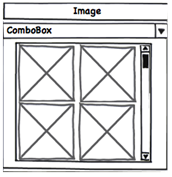
\includegraphics[scale=.6]{chap4/img-1}
\caption{Art�fact d'UI}
\label{fig:chap4:2}
\end{center}
\end{figure}


\begin{table}[h]
\begin{tabularx}{15cm}{|p{3cm}|Y|}
\hline  \textbf{Composants graphiques} & \textbf{Primitives d'interaction en entr�e}\\ 
\hline Liste d'images & 
			Widget Selection, Navigation, Widget Display, Data Selection,  Data Move Out, Activation \\ 
\hline Liste d�roulante & 
			Widget Selection, Navigation, Data Selection, Data Display, Activation \\ 
\hline 

\end{tabularx} 
\caption{Exemple de primitives d'interactions en entr�e}
\label{tab:chap4:1}
\end{table}


\subsection{Les primitives d'interactions en sortie}
\label{sec:chap4:2:2}
Elles d�crivent de mani�re abstraite les feed-back, les r�ponses ou les r�actions du NF sur les diff�rents �l�ments d'une UI. Elles concernent  le(s) contenu ou la repr�sentation d'un composant graphique. Nous avons identifi�s deux primitives d'interactions en sortie: la primitive d'interactions \hyperref[primitive:DD]{\textbf{Data Display}} et la primitive d'interactions \hyperref[primitive:WD]{\textbf{Widget Display}}

%\subsubsection{Primitives d'interaction concernant les donn�es }
\primitive{Data Display}{Elle permet d'exprimer la modification du contenu d'un �l�ment graphique par le NF}
\label{primitive:DD}
Certains composants graphiques sont utilis�s pour afficher des donn�es provenant du NF, cette primitive  exprime par exemple la possibilit� pour le NF de pr�senter des donn�es provenant du mod�le dans cas d'une architecture MVC par exemple. 

%\subsubsection{Primitives d'interaction concernant les composants graphiques}
\primitive{Widget Display}{Elle exprime les actions du NF  sur l'aspect visuel d'un composant graphique}
\label{primitive:WD}
Cette primitive d'interactions repr�sente la mise � jour des propri�t�s graphiques (visibilit�, position, taille) d'un composant graphique de la Vue par le Contr�leur ou Mod�le dans le cadre d'une architecture MVC par exemple.

\subsubsection{R�sum�}
Les primitives d'interactions en sortie caract�risent les r�actions et les feedback du NF sur les composants graphiques d'une UI.

Consid�rons par exemple la bo�te de dialogue de la figure~\ref{fig:messagebox} de l'application CBA, elle est affich�e apr�s une demande de fermeture d'une document. La bo�te de dialogue aura la primitive d'interactions \textbf{Widget Display} tels que d�crit dans le tableau~\ref{tab:chap4:2}. Le message est affich� dans un label qui obtient le nom du fichier � partir du mod�le, ce label aura donc la primitive d'interactions \textbf{Data Display}.

\begin{figure}[h]
\centering
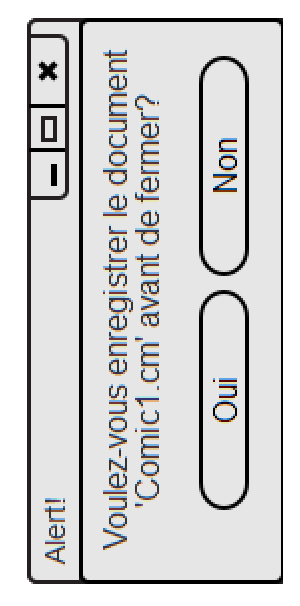
\includegraphics[angle=270, scale=.5]{chap5/messagebox}
\caption{Bo�te de dialogue}
\label{fig:messagebox}
\end{figure}


\begin{table}[h]
\begin{center}
\begin{tabular}{|p{3cm}|c|}
\hline  \textbf{Composants graphiques} & \textbf{Primitives d'interactions en sortie}\\ 
\hline Label Message & 	Data Display\\ 
\hline Bo�te de dialogue & 
			Widget Display \\ 
\hline 
\end{tabular} 
\end{center}
\caption{Exemple de primitives d'interactions en entr�e}
\label{tab:chap4:2}
\end{table}

\section[Composants graphiques]{Primitives d'interactions et Composants graphiques}
\label{sec:chap4:3}
%Cette section � pour objectif d'expliquer comment les PI des composants graphiques sont utiliser pour la migration et comment elle seront mod�liser � partir d'une UI finale.
Les composants graphiques appartiennent � des biblioth�ques graphiques (ou bo�tes � outils) et sont utilis�s pour d�crire des UI. Les composants graphiques qui constituent une UI sont des instances des composants graphiques d'une biblioth�que graphique. Les composants graphiques instanci�s n'impl�mentent pas syst�matiquement toutes les interactions possibles de son type. En consid�rant l'illustration de la figure~\ref{fig:instanceof} du lien entre une instance et son type d'une ListBox. De mani�re intrins�que, le composant ListBox d�finie les primitives d'interactions \textbf{Data Move Out} et \textbf{Data Move In} car il supporte l'interaction glisser-d�poser (drag-drop). Cependant de mani�re effective, il est possible de l'instancier sans impl�menter ces primitives d'interactions dans le cas d'une liste qui ne permet pas d'effectuer un glisser-d�poser de son contenu.

\begin{figure}[h]
\centering
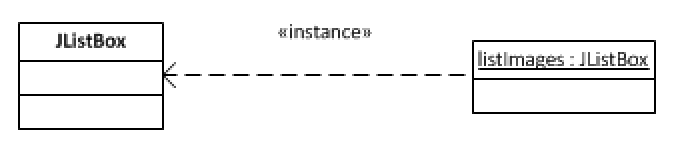
\includegraphics[ scale=.7]{chap5/instanceof}
\caption{Lien type-instance des composants graphiques}
\label{fig:instanceof}
\end{figure}

%\fbox{\parbox{0.9\textwidth}{
Nous constatons que pour des composants graphique qu'il existe des \textbf{primitives d'interactions intrins�ques} et des\textbf{ primitives d'interactions effectives}. %}}


Dans le cadre d'un processus de migration, l'on remarque aussi que pour les primitives d'interactions des �l�ments de l'UI � migrer sont des \textbf{primitives d'interactions effectives} car elles sont issues des instances des composants graphiques. Les composants graphiques de l'UI cible seront instanci�s � partir de la biblioth�que graphique de la plateforme d'arriv�e et ces instances devront conserv�s au moins les m�me primitives d'interactions que l'UI de d�part.


Les primitives d'interactions pr�sent�es � ci-dessus(cf. section~\ref{sec:chap4:2}) sont utilis�es pour d�crire l'ensemble des interactions possibles sur les composants graphiques. Elles font parties des mod�les abstraits d'UI avec les mod�les de structures, de layout et de styles. Les primitives d'interactions ne d�crivent pas les aspects structurels d'une UI tels que les types des donn�es, la cardinalit�s des donn�es ou le regroupement des composants graphiques. Dans notre processus de migration d'UI vers les tables interactives, nous nous basons sur deux mod�les abstraits (les primitives d'interactions et un mod�le de structure) pour d�crire les m�canismes automatiques de migration. Nous r�sumons les diff�rents �l�ments intervenants dans notre solution par la figure~\ref{fig:modelsutilises}, en effet l'UI finale est d�crite par des instances des �l�ments d'une biblioth�que graphique. Et les composants graphiques d'une biblioth�que graphiques sont d�crite par un mod�le de composant graphique g�n�rique, chaque composant graphique abstrait d�finit des primitives d'interactions intrins�ques. Par ailleurs les �l�ments d'une UI finale sont mod�lis�s � l'aide d'un mod�le de structure\footnote{Le mod�le de structure d�crit les types de donn�es, la cardinalit� des donn�es et le regroupement des �l�ments graphiques d'une UI} dont chaque instances impl�mente des primitives d'interactions effectives.  

Cette section pr�sente d'abord un mod�le de composant graphique ainsi que les r�gles qui permettent d'identifier les
\textbf{primitives d'interactions intrins�ques} � chaque composant graphique. Ensuite cette section pr�sente un mod�le de structure d'une instance d'UI ainsi que les r�gles d'identifications des \textbf{primitives d'interactions effectives}.


\begin{figure}[h]
\centering
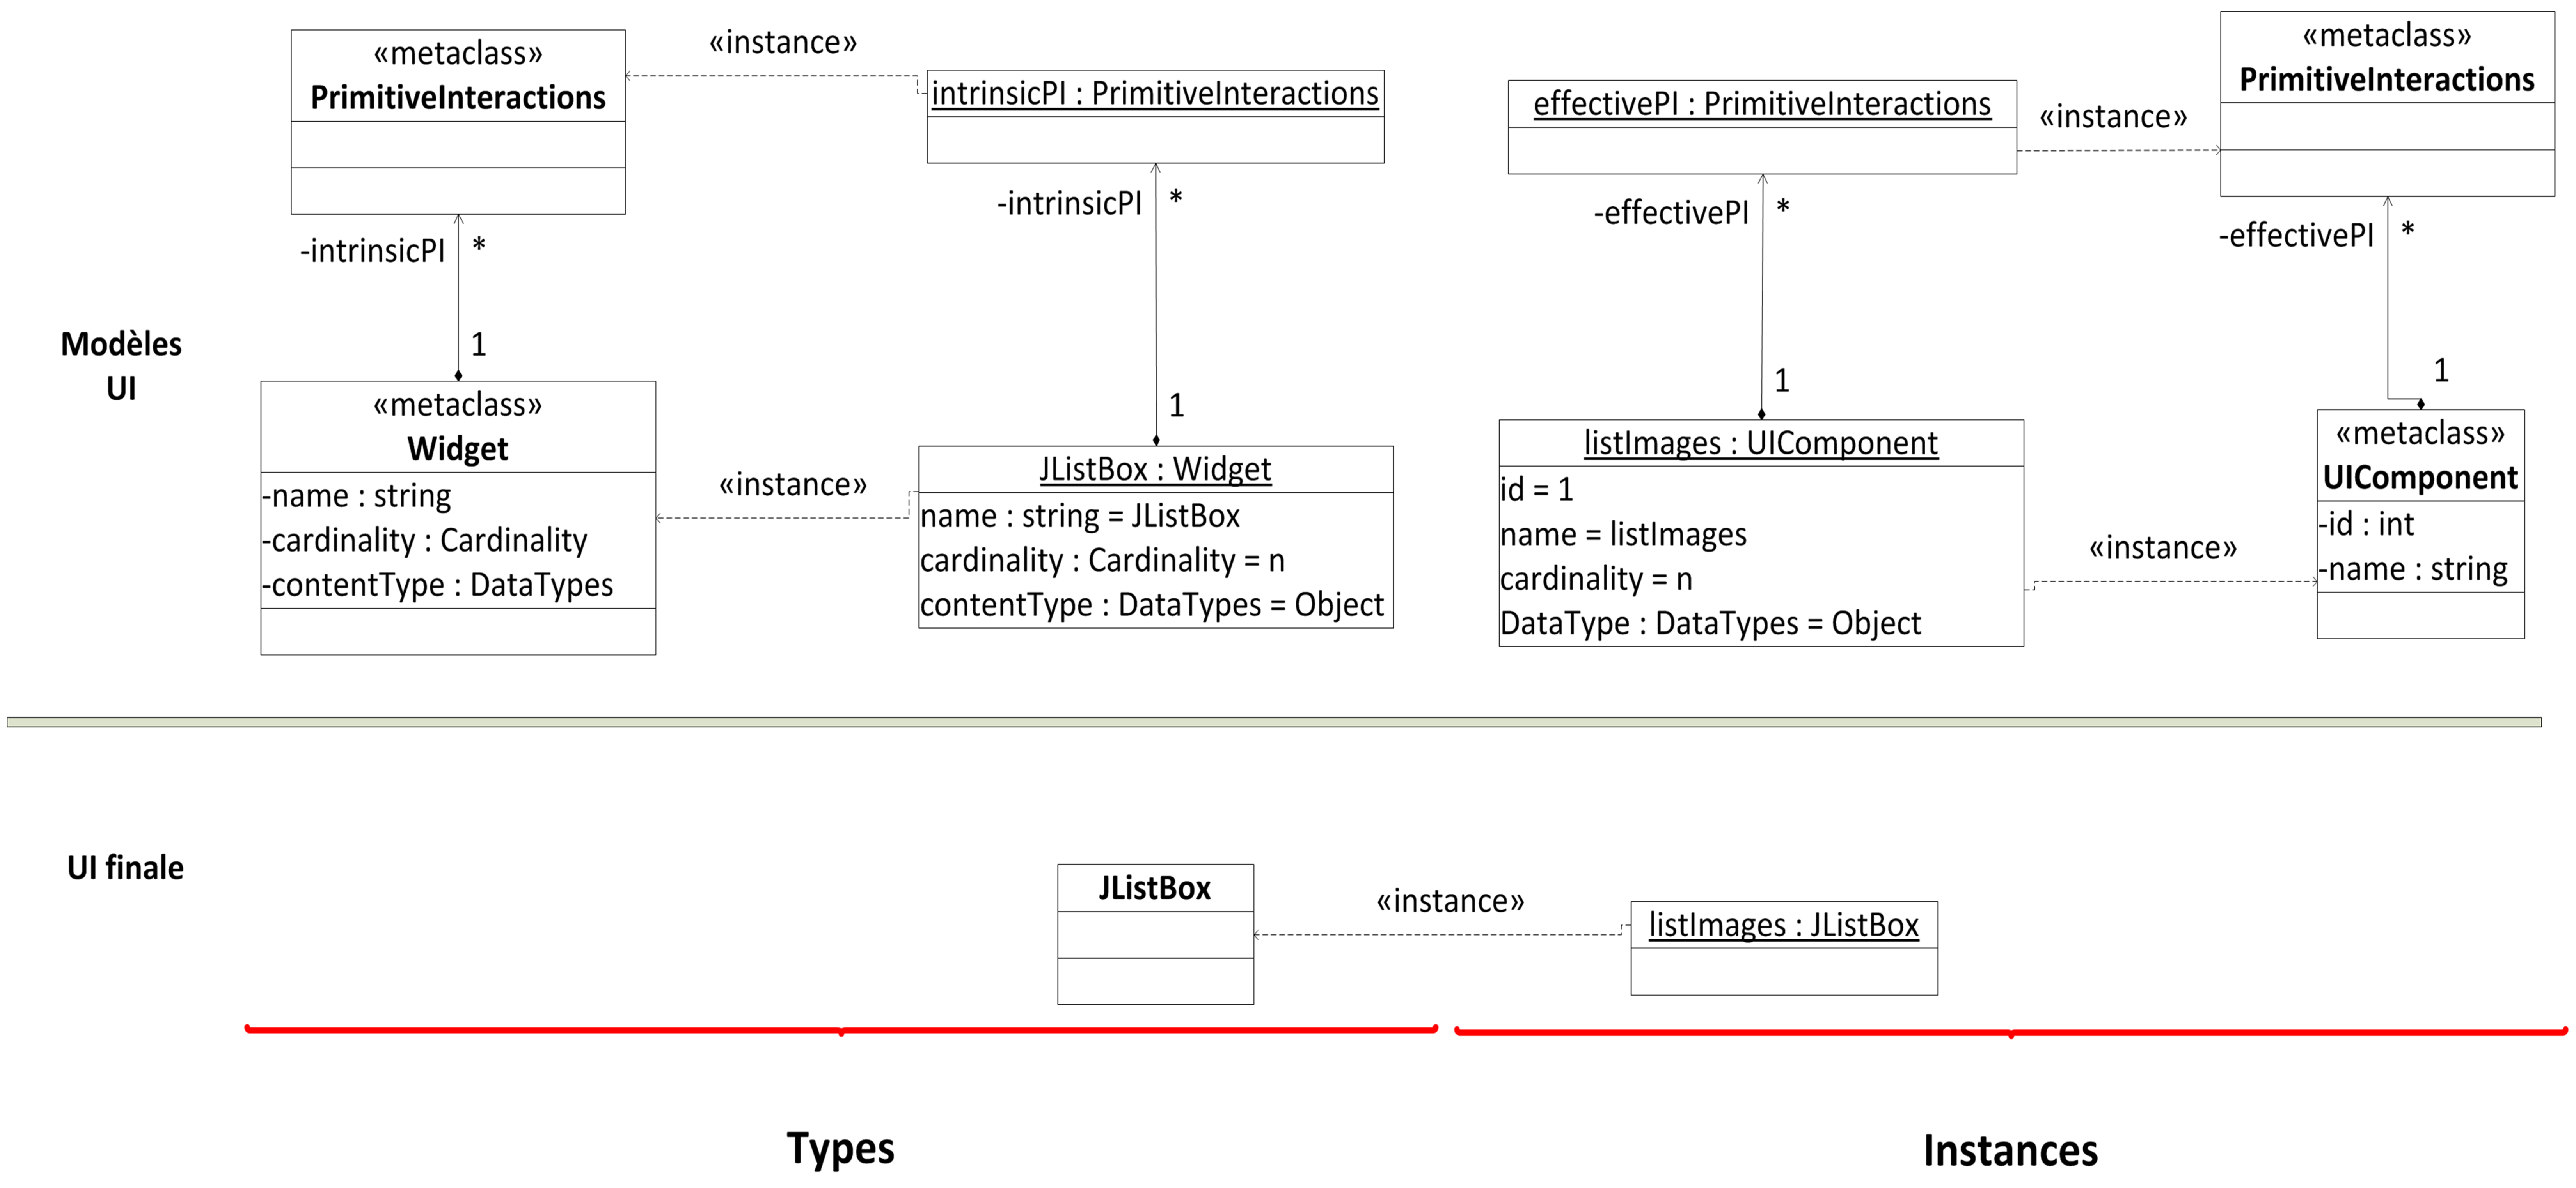
\includegraphics[ scale=.13]{chap5/modelsutilises-2}
\caption{Mod�les abstraits d'UI et UI finale}
\label{fig:modelsutilises}
\end{figure}

\subsection{Un mod�le abstrait de composants graphiques}
\label{sec:chap4:3:1}
Nous proposons dans cette section une formalisation des diff�rentes caract�ristiques d'un composant graphique dans un m�ta mod�le(cf figure~\ref{fig:chap4:3}), ceci dans le but de faciliter la d�finition des r�gles d'identification des primitives d'interactions des composants graphiques d'une UI � migrer.

\textit{``Widget is a user interface object which defines specific
interaction behaviour and a model of information presented to the user''}~\cite{December2001} 

Nous compl�tons cette d�finition en prenant en compte les caract�ristiques graphiques telles que la taille, la position, l'orientation et la structure du Widget. Nous ne consid�rons pas les caract�ristiques li�es aux styles de pr�sentation ou au layout car notre processus de migration permet aux d�veloppeurs de personnaliser l'UI pendant la migration. 

\begin{figure}[h]
\begin{center}
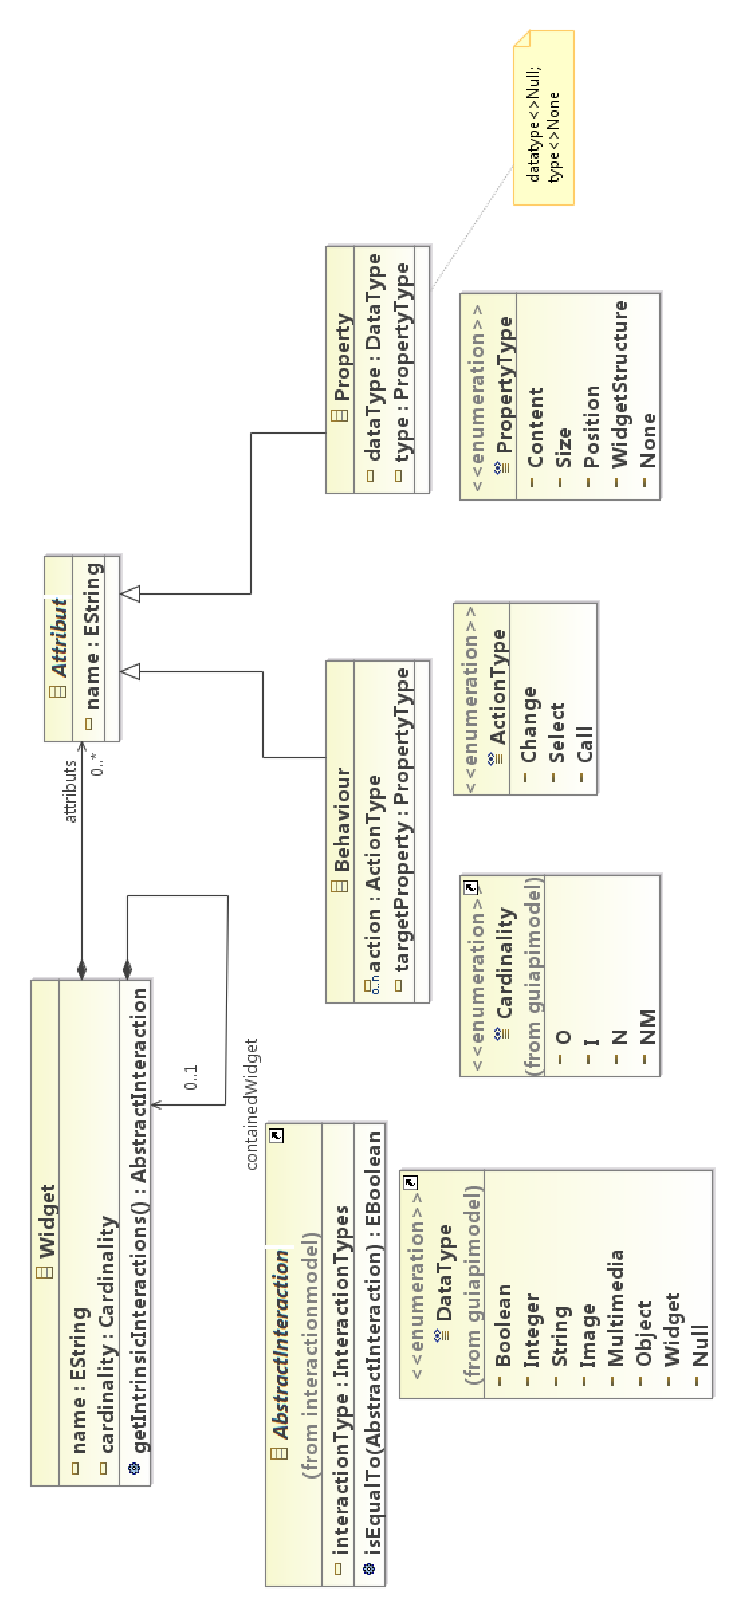
\includegraphics[scale=.6, angle=270]{chap4/widgetmodel}
\caption{M�ta mod�le de composant graphique}
\label{fig:chap4:3}
\end{center}
\end{figure}

\paragraph{Widget} Le m�ta mod�le de la figure 4-2 d�crit un composant graphique par la classe \textit{Widget} avec son nom (\textit{name}) et le nombre d'�l�ments qu'il peut contenir (\textit{cardinaltity}). Le champ \textit{name} permet de l'identifier de mani�re unique dans une biblioth�que graphique. La cardinalit� permet quand � elle de pr�ciser le nombre de donn�es ou de \textit{Widget} maximal qu'il peut contenir. Un composant graphique n�cessite dans certains cas d'autres composants graphiques pour ses contenus, l'association \textit{containedWidget} repr�sente les widgets utilis�s comme item. Par exemple en XAML~\cite{MicrosoftWPF2012} les ListBox n�cessitent des ListBoxItem. La classe Widget correspond � tous les composants graphiques d'une biblioth�que graphique.


\paragraph{Behaviour} Le m�ta mod�le de la figure~\ref{fig:chap4:3} consid�re que les comportements des composants graphiques consistent � modifier ou � s�lectionner son contenu, sa taille, sa position ou sa structure. Il consid�re aussi qu'un comportement fait aussi appel � des fonctionnalit�s. La classe \textit{Behaviour} est un attribut de \textit{Widget}, qui est caract�ris�e par les types de comportements (\textit{type}) et les propri�t�s qu'elle impacte (\textit{targetProperty}). Nous identifions trois types de comportements (\textit{BehaviorType)} parmi les caract�ristiques d'un \textit{Widget}~: 

\begin{enumerate}
\item  la modification (\textit{Change}) de valeurs du contenu (\textit{Content}), des propri�t�s graphiques (\textit{Size, Position,
Orientation}) 

\item  la s�lection (\textit{Select}) d'un contenu ou du Widget lui-m�me (\textit{WidgetStructure}) 

\item  et l'appel d'une fonctionnalit� (\textit{Call}).
\end{enumerate}

L'attribut \textit{targetProperty} de la classe \textit{Behaviour} permet de pr�ciser le type de propri�t� modifi�e par un comportement, dans le cas d'un comportement de type \textit{Call} alors ma propri�t� cible est nulle. Si un comportement est de type \textit{Select} alors la propri�t� cible est de type \textit{WidgetStructure} ou \textit{Content}. En effet la s�lection s'effectue uniquement  sur un composant graphique ou sur son contenu. Si un comportement est de type \textit{Change} alors la propri�t� cible est de type \textit{Size, Position, Orientation} ou \textit{Content}. En effet, le contenu, la taille, la position ou l'orientation d'un composant graphique sont modifi�s.

Un comportement peut combiner plusieurs types par exemple une liste
d�roulante permet de s�lectionner un item de la liste et aussi de d�clencher une
fonctionnalit�. Elle aura un attribut \textit{Behaviour} avec les types
\textit{Change} et \textit{Call} sur la propri�t� de type \textit{Content}. Un
\textit{Widget} peut avoir plusieurs comportements pour exprimer toutes ses
interactions intrins�ques, en effet les comportements d�crivent l'ensemble des
interactions possibles d'un composant graphiques, ces comportements sont
sp�cifiques � une biblioth�que graphique.

La classe \textit{Behaviour} est impl�ment�e de diff�rentes mani�res
par les biblioth�ques graphiques. Les comportements de type \textit{Change} et
\textit{Select} sont identifi�s en fonction des �v�nements, des m�thodes ou des
propri�t�s des composants graphiques. Par exemple en Java Swing, la propri�t�
\textit{isEditable} permet de dire qu'un composant graphique d�finit de mani�re
intrins�que un comportement pour changer son contenu. La m�thode
\textit{addActionListener} permet de dire qu'un composant graphique d�finit de
mani�re intrins�que un comportement pour faire appel � des fonctionnalit�s et la
m�thode \textit{getSelectedItem} permet de dire qu'un composant graphique d�fini
de mani�re intrins�que un comportement pour s�lectionner son contenu. Les
comportements de la biblioth�que graphique XAML sont identifi�s � partir des
�v�nements et des propri�t�s~; par exemple l'�v�nement \textit{SelectedText}
permet d'exprimer le comportement de s�lection d'un contenu, et la propri�t�
\textit{AllowDrop} permet d'exprimer que le contenu peut �tre chang�.

Pour chaque biblioth�que graphique, une table d�crivant les
correspondances entre les types de comportement et les caract�ristiques des
composants graphiques qui permet de les identifier de mani�re intrins�que est
fournie, des exemples de cette table sont d�crits de mani�re exhaustive pour les
biblioth�ques graphiques XAML et XAML Surface � l'annexe (r�f).


\paragraph{Property} La classe \textit{Property} (cf. figure~\ref{fig:chap4:3}) permet de d�crire les attributs
statiques des \textit{Widget}  qui sont impact�s par les comportements. Les
types des propri�t�s sont identifi�s de mani�re sp�cifique � chaque biblioth�que
graphique en d�crivant une correspondance entre les propri�t�s des composants
graphiques et les types de propri�t�s g�n�riques du m�ta mod�le de composant
graphique. Pour chaque biblioth�que graphique, il faut fournir les diff�rents
noms des propri�t�s des composants graphiques correspondant aux diff�rents types
(\textit{Content, Size, Position, Orientation, WidgetStructure}).

Les contenus d'un composant graphique sont de type
bool�en(\textit{Boolean}), entier (\textit{Integer}), cha�ne de
caract�re(\textit{String}), image (\textit{Image}), son ou vid�o
(\textit{MediaElement}), des classes ind�pendantes de la biblioth�que graphique
(\textit{Object}), des composants graphiques (\textit{Widget}). Tout autre type
n'est pas pris en compte par ce mod�le de composant graphique. L'identification
des types est faite � l'aide d'une table de correspondances entre les types
sp�cifiques aux biblioth�ques graphique et les types d�crit dans notre mod�le.
L'annexe (r�f) pr�sente des exemples de cette table de mani�re exhaustive pour
les biblioth�ques graphiques XAML et XAML Surface.

Le nom d'une propri�t� (tel que d�crit dans la biblioth�que graphique)
est conserv� pendant la migration (\textit{name)}, pour permettre � l'UI migr�
de pr�server les ressources (�tiquettes des widgets, etc.) de l'UI de d�part,
ceci permet de retrouver dans la structure analysable (\textit{UIStructure}) la
valeur de la propri�t� � partir de son nom.


\subsubsection{Identification des primitives d'interactions intrins�ques}

La m�thode $getIntrinsicInteractions: \{ Attributs\} \longrightarrow   \{AbstractInteraction\}$ du m�ta
mod�le (cf. figure~\ref{fig:chap4:3}) permet d'identifier les primitives d'interactions d'intrins�que d'un Widget. Cette m�thode se base sur des r�gles pour identifier chaque primitive d'interaction.


\idRule{Widget Selection et Navigation}{
\textbf{Widget Selection} et \textbf{Navigation}~sont d�finies de mani�re intrins�que pour tous les widgets.}

\idRule{Widget Resize}{  \textbf{Widget Resize} est d�finie de mani�re intrins�que pour tous les
widgets qui ont un comportement de changement des propri�t�s de type
\textit{Size}.\\
\[\exists prop\in Widget.attributs, prop.type=Size\]
\[ \bigwedge \]
\[\exists beh\in Widget.attributs beh.type=Change\] \[\bigwedge\] \[beh.targetProperty=Size \] }



\idRule{Widget Move}{ \textbf{ Widget Move} est d�finie de mani�re intrins�que pour tous les
widgets qui ont un comportement de changement des propri�t�s de type
\textit{Move.}\\
\[\exists prop\in Widget.attributs, prop.type=Position\] \[ \bigwedge \]
\[\exists beh \in Widget.attributs/beh.type=Change\bigwedge beh.targetProperty=Position \] }



\idRule{ Widget Rotation}{ \textbf{ Widget Rotation }est d�finie de mani�re intrins�que pour tous les
widgets qui ont un comportement de changement des propri�t�s de type
\textit{Orientation}. 
\[\exists prop\in Widget.attributs, prop.type=Orientation\]
\[\bigwedge\] 
\[\exists beh\in Widget.attributs/beh.type=Change \bigwedge evt.targetProperty=Orientation\] }



\idRule{Widget Display}{ \textbf{ Widget Display }est d�finie de mani�re intrins�que pour tous les
widgets.}



\idRule{Data Edition}{  \textbf{Data Edition} est d�finie de mani�re intrins�que pour tous les
widgets qui ont un comportement de changement des propri�t�s de type
\textit{Content }et dont le type de donn�es contenu n'est pas un
\textit{Widget.} \textit{ }\textbf{}
\[\exists prop\in Widget.attributs/prop.type=Content\] 
\[ \bigwedge \]
\[prop.dataType\notin \{Widget,\ Null\} \]
\[\bigwedge \] 
\[\exists beh\in Widget.attributs/beh.type=Change\ \bigwedge beh.targetProperty=Content\] }



\idRule{Data Selection}{ \textbf{ Data Selection }est d�finie de mani�re intrins�que pour tous les
widgets qui ont un comportement de s�lection des propri�t�s de type
\textit{Content}
\[ \exists prop\in Widget.attributs, prop.type=Content\] 
\[\vee \] 
\[ \exists beh\in Widget.attributs/beh.type=Select\wedge beh.targetProperty=Content \] }



\idRule{Data Move In}{ \textbf{ Data Move In} est d�finie de mani�re intrins�que pour tous les
widgets qui ont un comportement de changement des propri�t�s de type
\textit{Content}
\[\exists prop\in Widget.attributs/prop.type=Content\] 
\[ \bigwedge \]
\[ \exists beh\in Widget.attributs/ beh.type=Change\bigwedge beh.targetProperty=Content\] }



\idRule{Data Move Out}{ \textbf{ Data Move Out }est d�finie de mani�re intrins�que pour tous les
widgets qui ont un comportement de s�lection et de changement des propri�t�s de
type \textit{Content.} 
\[ \left\{ \begin{array}{c}
\exists {\mathbf \ }prop1\in Widget.attributs/\ prop1.type=Content\ \  \\ 
\wedge  \\ 
\exists beh1\in Widget.attibut\ /beh1.type=Select\  \\ 
\wedge \ beh1.targetProperty=Content \end{array}
\right\}\] 
\[\wedge \] 
\[\left\{ \begin{array}{c}
\exists {\mathbf \ }prop2\in Widget.attributs,\ prop2.type=Content\ \  \\ 
\wedge  \\ 
\ \exists {\mathbf \ }beh2\in Widget.attributs/beh2.type=Change\  \\ 
\wedge beh2.targetProperty=Content \end{array}
\right\}\]
\[ \wedge \] 
\[ prop1.valueDataType=prop2.valueDataType\]}



\idRule{Data Display}{ \textbf{ Data Display }est d�finie de mani�re intrins�que pour tous les
widgets qui ont des propri�t�s de type \textit{Content.} 
\[\exists {\mathbf \ }prop\in Widget.attributs/\ prop.type=Content\]  }



\idRule{Activation}{ \textbf{ Activation }est d�finie de mani�re intrins�que pour tous les
widgets qui ont des comportements de type \textit{Call} \textbf{}
\[\exists {\mathbf \ }evt\in Widget.attributs/beh.type=Call\] }



%Repr�sentation g�n�rique de la structure analysable d'une UI
\subsection{Un mod�le de structure d'UI}
\label{sec:chap4:4}

%L'utilisation des diff�rents mod�les~\cite{Demeure2007, Vanderdonckt2004}  pour la conception et l'adaptation~\cite{Favre2008,Kong1999} des UI a pour objectif de les d�crire ind�pendamment des plateformes~\cite{Brajnik2010} (dispositifs d'interaction en environnement
%logiciel). Ceci �vite aux concepteurs d'UI d'aborder tr�s t�t des questions
%li�es � l'impl�mentation telles que le choix des biblioth�ques graphiques, des
%widgets ou du style de pr�sentation. Dans notre contexte, la migration concerne
%les UI de modalit� graphique et permet d'adapter les UI des applications
%existantes � d'autres biblioth�ques graphiques. Les mod�les d'interface concr�te
%pr�sent�s au chapitre [r�f �tat de l'art] d�crivent des interacteurs qui
%permettent la repr�sentation des UI de la modalit� graphique ind�pendamment des
%biblioth�ques graphiques.
%
%Le processus de migration propos� dans ce manuscrit (r�f processus) a
%pour objectif d'assister les d�veloppeurs en charge d'adapter les UI sur des
%plateformes ayant des guidelines diff�rents. La structure analysable fournie en
%entr�e de ce processus (\textit{UIStructure}) est un arbre qui d�crit l'UI �
%l'aide des composants graphiques sp�cifiques � une biblioth�que graphique. Dans
%l'objectif d'adapter l'UI de d�part, nous avons extrait de la structure fournie
%une repr�sentation ind�pendante de la biblioth�que graphique qui d�crit la
%structure de l'UI � l'aide des composants graphiques instanci�s que nous
%appelons interacteurs~\cite{}. Cette repr�sentation nous permet de pr�ciser pour
%chaque interacteur les primitives d'interactions r�ellement utilis�es (primitives
%d'interaction effectives), les diff�rents groupes d'interacteurs et les
%ressources de l'UI � migrer. 

La structure des instances d'UI � migrer est d�crite sous diff�rents formats (XML, Archives Java, etc.) cependant tous ces formats peuvent �tre repr�sent�s � l'aide d'une structure arborescente. En effet, une fen�tre d'une UI peut �tre consid�rer comme la racine de l'arbre la repr�sentant et les �l�ments de la fen�tre seront des n\oe{uds fils. Si un ensemble de composants graphiques est regroup� dans un container alors ils seront repr�sent�s par n\oe{}ud parent correspondant au container et des n\oe{}ud fils correspondant aux composants de l'ensemble.

Les structures des UI sont mod�lis�es au niveau CUI du CRF~\cite{Calvary2002}, les diff�rents m�ta mod�le du niveau CUI~\cite{W3CIncubatorGroup2010, Vanderdonckt2004, Paterno'2009} caract�risent  entre autre les liens de contenance entre les �l�ments d'une UI, le cardinalit�s  et les types de donn�es que contiennent les composants graphiques. Les mod�les de CUI caract�risent aussi le style ou layout dans le cadre des UI graphiques, par exemple le langage UsiXML a plusieurs balises de layout pour le mod�le CUI  telque \textit{box, groupBox, flowBox}, etc.~\cite{Silva2012}.

%\fbox{\parbox{0.9\textwidth}{
Dans notre contexte, nous consid�rons qu'un mod�le de CUI capable de d�crire les liens de contenance, la cardinalit� et les types de donn�es d'une UI peut �tre utilis�s. Le but d'un mod�le de structure pour le processus de migration est de conserver les \textbf{donn�es} et  les \textbf{liens entre les composants graphiques} de l'UI de d�part. %}}

\begin{figure}[h]
 \begin{center}
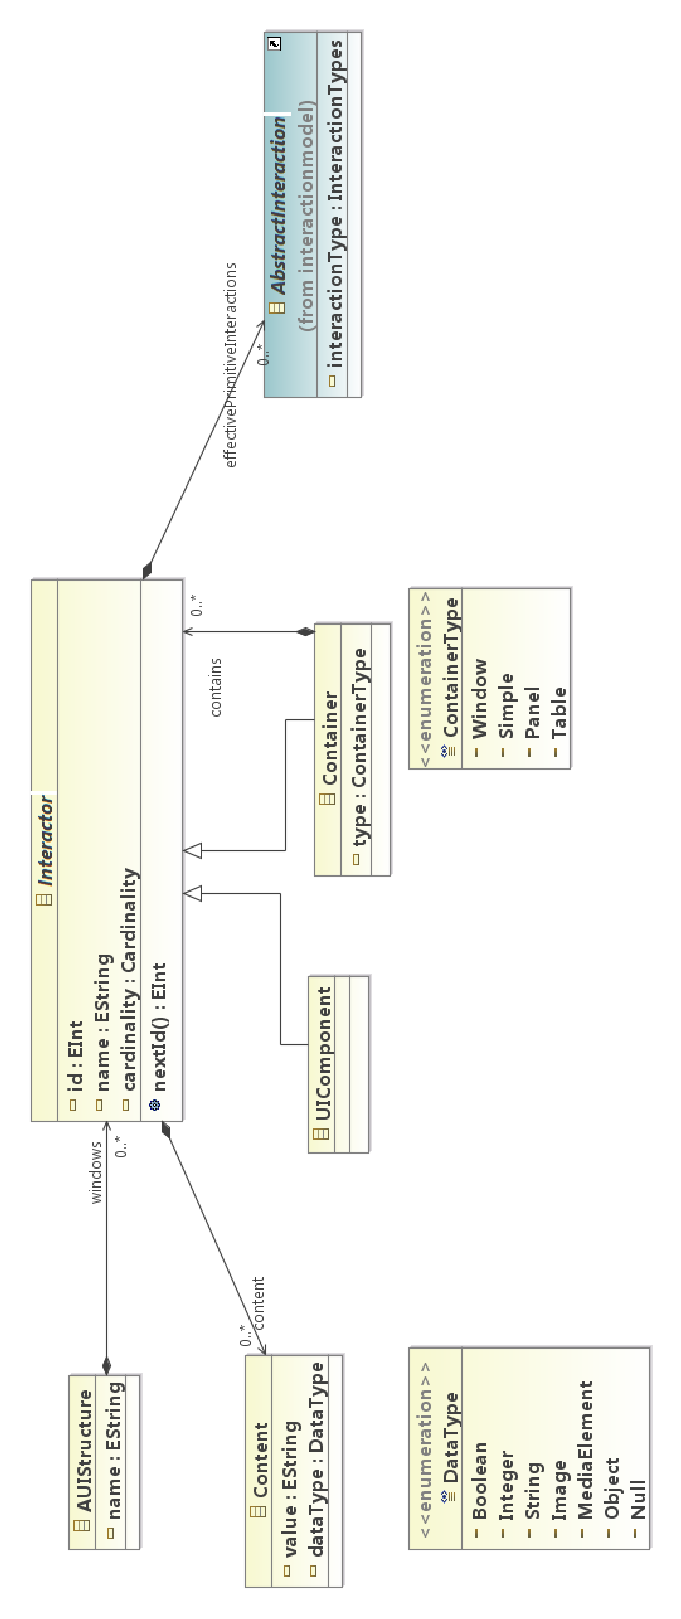
\includegraphics[angle=270, scale=.5]{chap4/interactormodel}
\caption{M�ta mod�le de structure}
\label{fig:chap4:4}
\end{center}
\end{figure}

Le mod�le de structure que nous utilisons pour la migration comporte des instances de composants graphiques d'une UI que nous repr�sentons dans un mod�le abstrait sous forme d'\textit{interacteurs}. Ces \textit{interacteurs} qui sont repr�sent�s par la classe abstraite \textit{Interactor} (cf. figure~\ref{fig:chap4:4}) sont caract�ris�es par leur identifiant unique pour une instance d'UI et leur nom qui correspond au nom du composant graphique de l'UI � migrer. Ils pr�servent les valeurs des donn�es structurelles de l'UI � migrer par la classe \textit{Content} , par exemple les �tiquettes des labels, des boutons, des images, etc. On distingue deux types d'instances de widgets : 

\begin{itemize}
\item  \textit{UIComponent} repr�sentant l'ensemble des composants graphiques ne pouvant pas contenir de composant graphique. Ils sont identifi�s � partir des widgets dont les contenus ne sont pas d'autres widgets,

\item  et \textit{Container} repr�sentant l'ensemble des composants graphiques pouvant contenir d'autres instances de widgets. Ils sont identifi�s � partir des widgets pouvant contenir d'autres widgets. 
\end{itemize}

\subsubsection{Types de Container}
Les Container peuvent �tre cat�goris�s en fonction des interacteurs qu'ils contiennent. Nous caract�risons dans le  tableau~\ref{tab:chap4:3} quatre types de container. Les types de containers sont identifi�s � partir de la structure d'une UI de mani�re r�cursive en identifiant d'abord les types des interacteurs fils.

\begin{table}[t]
\begin{tabularx}{15cm}{|Y|Y|}
\hline   Contenu &  Type de container \\
\hline  $\{UIComponent\}$ & 
  \textbf{Homog�ne}: donn�es du m�me type \newline \textbf{H�t�rog�ne}: donn�es de type diff�rents \newline \textbf{Racine}: si pas de parent  \\ 
\hline  $\{ UIComponent\}\cup \{Container\} $ &
\textbf{H�t�rog�ne:} si a un parent \newline \textbf{Racine}: si pas de parent\\ 
\hline $ \{Container\} $ & \textbf{R�cursif:} si contient des containers \newline \textbf{Racine}: si pas de parent\\ 
\hline 
\end{tabularx} 
\caption{Types de container}
\label{tab:chap4:3}
\end{table}


%{|p{0.7in}|p{0.9in}|p{1.1in}|p{0.8in}|p{0.7in}|}
%{|p{3.4in}|}
%\begin{table}[h]
%\begin{tabularx}{15cm}{|Y|Y|Y|Y|Y|} 
%\hline 			& \multicolumn{4}{|c|}{\textbf{Types de container}} \\ 
%\hline  \textbf{El�ments du container} 
%				& \textbf{Table} 
%				& \textbf{Panel} 
%				& \textbf{Simple} 
%				&  \textbf{Window} \\  
%\hline \textit{$$ \left\{ UIComponent \right\} $$}
%				& Si tous ses interacteurs ont des contenus de m�me type. 
%				& \centering Si tous les interacteurs n'ont pas de contenu  Ou  Si les contenus ne sont pas de m�me type 
%				& \cellcolor{green!7} Le container  n'est pas de type Simple 
%				&    \\ \cline{1-4}
%\cline{1-4} \textit{ $$\left\{  Container \right\}$$  } 
%				& \cellcolor{green!7} \centering Le container  n'est pas de type Table \newline  
%				& \cellcolor{green!7} \centering  Le container n'est pas de type Panel 
%				& \centering Si tous ses interacteurs sont des Container  
%				&  \\ 
%\cline{1-4} \textit{ $$\left\{ UIComponent \right\}$$ }
%				\newline $$\cup $$ \newline \textit{ $$ \left\{ Container \right\}$$ } 
%				& \cellcolor{green!7}  \centering Le container  n'est pas de type Table 
%				& \centering Si tous les interacteurs ne sont pas des Container mais des \textit{ UIComponent} aussi 
%				&  \cellcolor{green!7} \centering Le container  n'est pas de type Simple 
%				& \multirow{-3}{2cm}{\centering Si le container  est l'�l�ment racine d'une UI } \\
%\hline 
%\end{tabularx}
%
%\caption{Types de container}
%\label{tab:chap4:3}
%\end{table}

\paragraph{Container Racine}C'est la d'une structure d'UI. Il peut contenir des containers et des interacteurs simple.

\paragraph{Container R�cursif}C'est un container ne contenant que des \textit{Container}. Ce type permet d'identifier un regroupement de plusieurs containers sur le quel on pourra appliquer des transformations. Un container de type \textit{R�cursif} ne peut donc pas contenir des interacteurs de types \textit{UIComponent}. En consid�rant la figure~\ref{fig:chap4:5}, le container vert de est une illustration d'un \textit{Container} de type \textit{R�cursif}. 


\paragraph{Container Homog�ne}C'est un container contenant uniquement des \textit{UIComponent} dont les donn�es du m�me type et de m�me cardinalit�. Un container de ce type permet de d�finir un groupe de composants graphique de m�me type (tel qu'une liste, un tableau, un menu, etc.). Le container bleu de la figure~\ref{fig:chap4:5} est une illustration d'un \textit{Container} de type \textit{Homog�ne}.

\paragraph{Container H�t�rog�ne}C'est un container pouvant contenir � la fois des\textit{UIComponent} et des \textit{Container}. Ce type permet d'identifier les instances de widgets pouvant contenir des donn�es non structur�es et qui sont interpr�t�s de diverses mani�res pendant la migration. En consid�rant la figure~\ref{fig:chap4:5} Le container rouge est une illustration d'un \textit{Container} de type \textit{H�t�rog�ne}. 
%[width=5.01in, height=3.16in,keepaspectratio=false]

\begin{figure}[h]
 \begin{center}
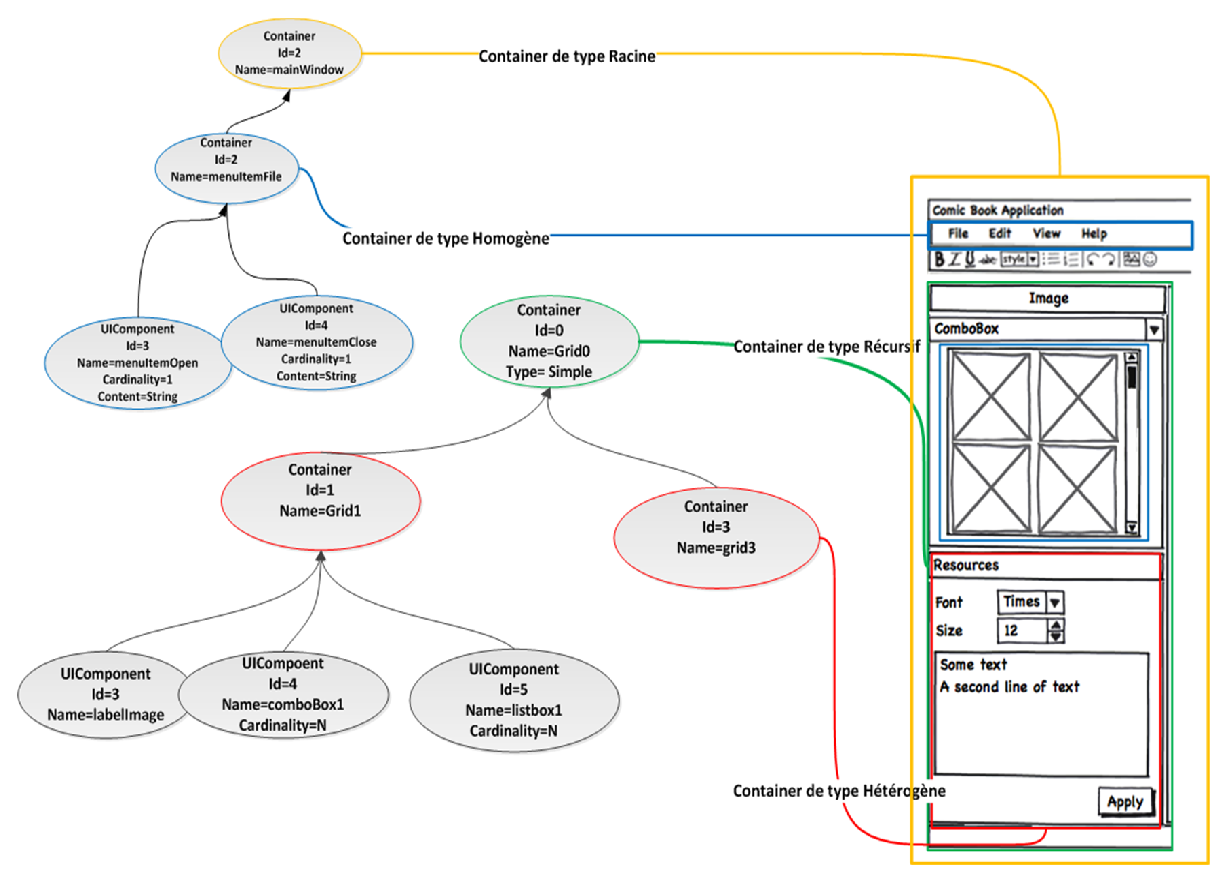
\includegraphics[scale=.8]{chap4/typecontainers}
\caption{Illustration des types de container}
\label{fig:chap4:5}
\end{center}
\end{figure}


\subsubsection{Donn�es des interacteurs}
Le mod�le de structure pr�sent� � la figure~\ref{fig:chap4:4} permet de pr�server les donn�es d'une UI � migrer. Le processus de migration dans notre cas permet un changement de la modalit� d'interactions mais les donn�es contenues dans une UI ou �chang�es entre l'UI et NF doit �tre pr�server car le NF est r�utilis�s.

Le mod�le de structure~\ref{fig:chap4:4} propose un ensemble de type de donn�es classiques d'UI. \textit{DataType} est consid�r� comme un mod�le de type de donn�es abstrait qui sera instanci� en fonction de chaque langage de programmation. Par exemple le type \textit{MediaElement}  repr�sente un objet de type vid�o et le type \textit{Object}  d�signe des types complexes.


\subsubsection{Primitives d'interactions effectives}
Les primitives d'interactions r�ellement utilis�es par chaque interacteur sont identifi�es � partir de la structure de l'UI de d�part. Cependant pour pr�server l'assemblage des composants graphiques de l'UI � migrer, on extrait au moyen d'interacteurs cette structure arborescente � l'aide du m�ta mod�le \textit{AUIStructure}. Il d�crit la structure de l'UI comme un ensemble d'arbre dont les racines sont des fen�tres, les n\oe{}uds des interacteurs et les arcs la relation de contenance entre les interacteurs. Chaque interacteur a une m�thode qui permet d'identifier les primitives d'interactions effectives en fonction du n\oe{}ud correspondant dans la structure analysable de d�part et du mod�le de \textit{Widget}.


On consid�re que l'UI de d�part est une structure analysable \textit{UIStructure} qui est constitu� d'un ensemble d'arbres (\textit{Tree}) qui d�crit les diff�rentes fen�tres de l'UI � migrer.
\[UIStructure=\ \bigcup^N_{i=0}{Tree_i}\] 
\[Tree_i=\left\langle root,\ Node,\ Contains\right\rangle \ \ \] 


%\setcounter{idRul}{0}

La m�thode $getEffectiveInteractions: WidgetNode \rightarrow\ \left\{AbstractInteraction\right\} $ du m�ta mod�le (cf. figure~\ref{fig:chap4:3}) permet d'identifier les primitives d'interactions utilis�es par un interacteur. Cette
m�thode se base sur des r�gles effectives suivantes.

%\begin{enumerate}

\idRule{Widget Selection et Navigation}{
\textbf{Widget Selection} et \textbf{Navigation}~sont d�finies de mani�re
effective pour les interacteurs accessible dont les propri�t�s de type
\textit{WidgetStructure}(cf. figure~\ref{fig:chap4:3})sont de type bool�en et avec une valeur diff�rente de
false.\\
\[ \exists prop \in Widget.attributs, prop.type=WidgetStructure \]
\[\wedge\]
\[ \exists att\in{Node}/prop.dataType=Boolean \]
\[\wedge\]
\[ att.name=prop.name\wedge node.value\ne False\]
}

\idRule{Widget Resize}{
\textbf{Widget Resize} est d�finie de mani�re effective pour les
interacteurs redimensionnables dont les propri�t�s de type \textit{Size} sont de
type bool�en et avec une valeur diff�rente de false.\\
\[\exists prop\in Widget.attributs, prop.type=Size \]  
\[\wedge\] 
\[\exists att\in {Node}/prop.dataType=Boolean \]
\[\wedge \] 
\[ att.name=prop.name\wedge node.value\ne False\ \] 
}


\idRule{Widget Mode}{ \textbf{ Widget Move} est d�finie de mani�re effective pour les
interacteurs d�pla�ables dont les propri�t�s de type \textit{Move} sont de type
bool�en et avec une valeur diff�rente de false.\\
\[ \exists prop\in Widget.attributs, prop.type=Move\] 
\[\wedge\] 
\[\exists att\in{Node}/prop.dataType=Boolean\]
\[\wedge\]
\[ att.name=prop.name\wedge node.value\ne False \]
}

\idRule{Widget Rotation}{\textbf{ Widget Rotation }est d�finie de mani�re effective pour les
interacteurs orientables dont les propri�t�s de type \textit{Orientation} sont
de type bool�en et avec une valeur diff�rente de false.\\
\[ \exists prop\in Widget.attributs, prop.type=Orientation\]
\[\wedge\]
\[ \exists att\in {Node}/prop.dataType=Boolean\] 
\[\wedge\]
\[ att.name=prop.name\wedge node.value\ne False\ \] }

\idRule{Widget Display}{\textbf{Widget Display }est d�finie de mani�re effective pour tous les
interacteurs.}\\



\idRule{Data Edition}{\textbf{Data Edition}est d�finie de mani�re effective pour tous les interacteurs
accessibles dont les widgets pour lesquels la primitive est d�finie de mani�re
intrins�que.}


\idRule{Data Selection} {\textbf{ Data Selection }est d�finie de mani�re effective pour tous les
interacteurs accessibles dont les widgets pour lesquels la primitive est d�finie
de mani�re intrins�que.}


\idRule{Data Move In}{\textbf{ Data Move In} est d�finie de mani�re effective pour tous les
interacteurs accessibles dont les widgets pour lesquels la primitive est d�finie
de mani�re intrins�que}


\idRule{Data Move Out}{\textbf{ Data Move Out }est d�finie de mani�re effective pour tous les
interacteurs qui d�finissent de mani�re effective \textbf{Data Selection} et
\textbf{Data Edition}.}


\idRule{Data Display}{\textbf{Data Display }est d�finie de mani�re effective pour tous les
interacteurs qui ont un contenu ou dont la propri�t� de contenu est modifi�e
dans une m�thode. \textbf{}}


\idRule{Activation}{ \textbf{ Activation }est d�finie de mani�re effective pour tous les interacteurs qui font appel � une m�thode du contr�leur (dans une architecture MVC)}}



\subsection{Synth�se des mod�les abstraits}
% Faire la synth�se des mod�les pr�sent� et dire � quoi ils vont servir pour la suite dans le processus de migration
Cette section a pr�sent� un mod�le de composants graphiques et un mod�le de structure pour une instance d'UI. Le mod�le de composant graphique d�crit de mani�re abstraite tous les aspects des widgets d'une biblioth�que graphique. En effet, le m�ta mod�le de la figure~\ref{fig:chap4:3} d�crit le contenu, la cardinalit�, les propri�t�s graphiques (position et taille), les comportements et les interactions d'un composant graphique ind�pendamment de sa repr�sentation par une bo�te � outils donn�e.
 
Par ailleurs le mod�le de structure (cf. figure~\ref{fig:chap4:4}) repr�sente les liens de contenances et les donn�es d'une instance d'UI � migrer. Ce mod�le est certes compos� d'instances de composants graphiques mais il ne d�crit pas tous les aspects d'une UI.
% Nous formalisons le lien entre un mod�le de composant graphique et un mod�le de structure par la fonction $instanciateUIStructure:UIStructure\times \{Widget\} \to AUIStructure$ qui permet d'abstraire le mod�le de structure d'une UI de d�part. 

Dans le cadre de la migration, les applications � migrer sont abstraits dans le mod�le de structure \textit{AUIStructure} en exprimant aussi les primitives d'interactions effectives. L'application source ainsi abstrait est transform�e pour �tre conforme aux recommandations de la plateforme cible. La section suivante pr�sente le m�canisme de migration bas�e sur les primitives d'interactions et les mod�les d�crits dans cette section.
 

\section[Op�rateurs d'�quivalences ]{Op�rateurs d'�quivalences des composants graphiques bas�s sur des primitives d'interactions}


Les \textit{Widget} ou \textit{Interactor} sont caract�ris�s respectivement par leurs primitives interactions intrins�ques et effectives qui sont des sous-ensembles des primitives d'interactions. Nous d�finissons trois op�rateurs de comparaisons de ces sous-ensembles de primitives d'interaction: l'�galit�($=$), l'inclusion($\subseteq$) et la contenance($\supseteq$).

\paragraph{�galit� des deux sous ensemble de primitives d'interactions\\}  
$=:\{PrimitiveInteractions\}\times \{PrimitiveInteractions\}\to Boolean$.\\
Si toutes les primitives d'interactions de deux sous-ensemble sont identiques.

\paragraph{Inclusion des primitives d'interactions\\}
$\subseteq:\{PrimitiveInteractions\}\times \{PrimitiveInteractions\}\to Boolean$\\
Si toutes les primitives d'interaction du sous ensemble de gauche se retrouvent dans le sous-ensemble de droite. Ceci est possible si une instance de \textit{Widget} n'utilise pas toutes ses primitives d'interaction intrins�ques.

\paragraph{Contenance des primitives d'interactions\\} 
$\supseteq :\{PrimitiveInteractions\}\times \{PrimitiveInteractions\}\to Boolean$ \\
Ceci est possible si la biblioth�que graphique ne contient pas de widgets avec le sous ensemble de primitives d'interaction intrins�ques �quivalent � l'interacteur. Dans ces cas on consid�re les widgets qui n'impl�mentent pas les primitives d'interactions concernant les propri�t�s graphiques tout en conservant les autres primitives d'interactions. Les primitives d'interaction \textbf{Widget Move}, \textbf{Widget Rotation} et \textbf{Widget Resize} sont les seules qui peuvent �tre omis par l'op�rateur de comparaison$\supseteq $.

%TODO: A quoi sevent ces op�rateurs?

\subsection{�quivalences des interacteurs}

La s�lection est un processus qui permet de retrouver l'ensemble des
widgets �quivalents � un interacteur dans la biblioth�que graphique de la
plateforme d'arriv�e. Ce processus se base sur des op�rateurs de comparaison qui
permettent d'�tablir les �quivalences entre les interacteurs et les widgets.
Cette section pr�sente les diff�rents op�rateurs de comparaison et l'algorithme
de s�lection des widgets �quivalents.


\subsubsection{Les op�rateurs de comparaison}

La comparaison entre les interacteurs et les widgets se basent sur les
caract�ristiques qui leurs sont communes telles que les primitives
d'interactions (effectives et intrins�ques), le type et la cardinalit� de
donn�es. 

La comparaison des cardinalit� est effectu�e pour v�rifier si les
widgets �quivalents supportent le m�me nombre de donn�es que l'interacteur �
migrer. Elle est possible gr�ce � la fonction $equalCard:Interactor\times Widget\to Boolean.\ \forall i\in \left\{Interactor\right\}\wedge \forall w\in \left\{Widget\right\},$
\[equalCard\left(i,w\right)=\left\{ 
\begin{array}{l}
	True,\ i.content.Cardinality=w.Cardinality \\ 
	False,\  else  
\end{array} \right.\ \] 
La prise en compte de la caract�ristique types de donn�es pour comparer les
interacteurs et les widgets � pout but de v�rifier si l'adaptation des widgets
�quivalents n�cessite l'ajout d'un adaptateur de types de donn�es. En effet si
la cardinalit� et les primitives d'interaction d'un \textit{Widget}
correspondent � ceux d'un interacteur alors ce Widget sera propos� au concepteur
comme �quivalent m�me si son utilisation n�cessite un travail suppl�mentaire
(�criture du code pour adaptateur de type).

La fonction $equalDataType:Interactor\times Widget\to Boolean$ permet v�rifier l'�galit� des types de donn�es des interacteurs et des
widgets. $\forall  i \in \left\{Interactor\right\},\forall w\in \left\{Widget\right\},\ $
\[equalDataType(i ,w )=\left\{
\begin{array}{l}
	True, \left(\genfrac{}{}{0pt}{}{
				\begin{array}{l}
					\begin{array}{c}
						\exists att\in w.attibuts,\\
						i.Content.dataType=att.dataType\\
					\end{array}
				\end{array}}
			{\begin{array}{l}
				\begin{array}{c}
					\vee  \\ 
					i.Content.dataType=Null \\ 
					\wedge  \\ 
					\nexists att \in w.{attibuts}/{att.type=Content}\  
				\end{array}
			\end{array}
		}\right) \\ 
 	\\ 
	False , else  
\end{array}
\right.\] 


Les op�rateurs de comparaison combinent les trois caract�ristiques en consid�rant d'abord la cardinalit� des donn�es, car il n'y a pas d'�quivalence entre un interacteur et un Widget s'ils n'ont pas la m�me cardinalit�. Ensuite, les op�rateurs consid�rent les types des donn�es des interacteurs et enfin les sous-ensembles de primitives d'interaction. La combinaison des ces op�rateurs des caract�ristiques nous permet de relever quatre cas d'�quivalences signifiant pour le processus de migration~: le cas d'une �quivalence stricte suivant les trois caract�ristiques ci-dessus, le cas d'une �quivalence
large , le cas d'une �quivalence simple et le cas d'une �quivalence faible (6.2.1.4).


\subsubsection{�quivalence stricte }

\begin{flushleft}
Il ya une �quivalence stricte entre un interacteur et un Widget s'ils ont des
cardinalit�s �gales, les m�me types de donn�es et des primitives d'interaction
�gales. La fonction$\ {\mathbf strongEquivalent}{\rm \ }:Interactor\times
Widget\to Boolean$\textit{ }permet de v�rifier cette �quivalence, $\forall \ i\
\in \left\{Interactor\right\},\forall w\in \left\{Widget\right\},\ $
\[ strongEquivalent (i,w ){\rm =}\left\{ 
	\begin{array}{l}
		True {\rm ,\ }\left(\genfrac{}{}{0pt}{}
						{\begin{array}{c}
							 equalCard\left(i, w\right) \\
							 \wedge  \\ 
							 equalDataType\left( i, w \right) \\ 
						\end{array}}
						{ \begin{array}{c}
							\wedge  \\ 
							i =w
						\end{array}
					}\right) \\ 
			{\rm \ \ } \\ 
		False, else 
	\end{array}
\right.\ \] 
\end{flushleft}


\subsubsection{Equivalence large}

\begin{flushleft}
Il y a une �quivalence large entre un interacteur et un Widget s'ils ont des
cardinalit�s �gales,  les m�mes types de donn�es et si les primitives
d'interaction de l'interacteur sont incluses dans celles du Widget. La fonction
${\mathbf largeEquivalent}{\rm \ }:Interactor\ X\ Widget\to Boolean$ permet de
v�rifier cette �quivalence.$\forall \ i\ \in \left\{Interactor\right\},\forall
w\in \left\{Widget\right\},\ $
\[ largeEquivalent ( i,w ){\rm =}
	\left\{ 
		\begin{array}{l} True {\rm ,\ }
		\left(\genfrac{}{}{0pt}{}{
			\begin{array}{c}
				equalCard\left(i,w \right) \\
				\wedge  \\
				equalDataType \left(i,w \right) \\ 
			\end{array}}
			{ \begin{array}{c}
				\wedge  \\ 
				i\subseteq w 
			\end{array}}
		\right) \\ 
		{\rm \ \ } \\ 
		False, else 
		\end{array}
	\right.\] 
\end{flushleft}


\subsubsection{�quivalence simple}

\begin{flushleft}
Il y a une �quivalence simple entre un interacteur et un Widget s'ils ont des
cardinalit�s �gales,  les types de donn�es diff�rentes et si les primitives
d'interaction de l'interacteur sont �gales ou incluses dans celles du Widget. La
fonction $simpleEquivalent \ :Interactor\ X\ Widget\to Boolean$ permet de v�rifier cette �quivalence. $\forall \ i\ \in
\left\{Interactor\right\},\forall w\in \left\{Widget\right\},$
\[ simpleEquivalent( i , w ) = \left\{ 
			\begin{array}{l}
				 True, \left(\genfrac{}{}{0pt}{}{
				 	\begin{array}{c}
						equalCard\left( i, w \right)\\
						\wedge  \\ 
						!equalDataType\left(i,w \right) \\ 
						\wedge  \\ 
					\end{array}}
					{ \begin{array}{c}
						\left(i \subseteq w \vee i=w \right) 
					\end{array}}
				\right) \\
				\\  
				False, else 
			\end{array}
\right.\] 

\end{flushleft}


\subsubsection{�quivalence faible}

\begin{flushleft}
La fonction $lowEquivalent:Interactor\ X\ Widget\to Boolean$ permet
de v�rifier cette �quivalence. $\forall \ i\ \in \left\{Interactor\right\},\forall w\in \left\{Widget\right\},$
\[ lowEquivalent (i,w) =\left\{
			\begin{array}{l}
				True, \left(\genfrac{}{}{0pt}{}{ 
					\begin{array}{c}
						equalCard ( i,w )\\
						\wedge  \\ 
						!equalDataType (i,w)\\ 
						\wedge  \\ 
					\end{array}}
				{ \begin{array}{c}
					( i \supseteq w ) 
				\end{array}}
				\right) \\ 
				False
			\end{array}
\right.\] 
\end{flushleft}


\subsection{Correspondances entre interacteurs et composants graphiques}


\section{Synth�se}
\label{sec:chap4:5} \textbf{[TODO]}
Les primitives d'interaction pr�sent�es dans ce chapitre permettent la repr�sentation des interactions intrins�ques aux composants graphiques et effectives aux interacteurs. Cette repr�sentation offre des �l�ments de comparaison entre interacteurs de l'UI � migrer et les composants graphiques de la plateforme d'arriv�e. Les algorithmes d'�quivalence utilis�s par le processus de migration s'appuient sur les primitives d'�quivalence pour la s�lection des widgets correspondants aux interacteurs � migrer. 
Les interacteurs permettent de d�crire les instances d'UI et leurs interactions effectives ind�pendamment des biblioth�ques graphiques  tout en conservant leurs ressources et les liens entre eux. La structure analysable \textit{UIStructure} fournie en entr�e est repr�sent�e de mani�re abstraite par un ensemble d'arbre d'interacteurs. 

Cette structure abstraite est utilis�e par le processus de migration pour �tablir les �quivalences avec les widgets de la plateforme cible et pour  identifier et transformer les groupes d'interacteurs en fonction des guidelines.   
Par ailleurs cette mod�lisation des interactions et de la structure des �l�ments d'une UI ne prend pas en compte toutes les pr�occupations li�es � la conception des UI adaptables aux contextes d'usage telles que d�finies par CRF. En effet, les mod�lisations pour l'adaptation des styles de pr�sentation de l'UI [r�f style], du layout [r�f layout] des composants graphiques ou des comportements de l'UI de fa�on globale [r�f t�che] ne sont pas prises en compte dans la mod�lisation propos�e dans ce chapitre. Le processus de migration que nous proposons permet aussi d'assister les d�veloppeurs pendant le choix des styles et pr�sentation ou du layout suivant les guidelines de la plateforme d'arriv�e.  


	%
	\chapter{Mod�lisation des UI }
	%\label{chap5}
	%\minitoc
	%%\section{Introduction}
\label{sec:chap5:1}
La solution de migration assist�e que nous proposons est constitu�e de
trois phase~: la phase d'extraction � partir de la structure analysable
(\textit{UIStruture}) d'une repr�sentation (\textit{AUIStructure})  qui est
d�crite dans le chapitre pr�c�dent, la phase d'adaptation de la structure de
l'UI aux r�gles ergonomiques de la table interactive et enfin la phase de
projection du mod�le d'UI adapt�, cette phase permet aussi aux concepteurs de
personnaliser l'UI finale.   


\section{Adaptation de la structure de l'UI }

Cette phase a pour finalit� la production d'une structure d'UI adapt�e
aux r�gles ergonomiques de  la table interactive. L'adaptation du mod�le de
structure (\textit{AUIStructure}) extraite de l'UI � migrer se fait en fonction
des r�gles ergonomiques que nous pr�sentons � la section 6.2.1.  La section
6.2.2 pr�sente une formalisation des r�gles d'adaptation de la structure et
enfin la section 6.2.3 est une synth�se du processus d'adaptation de la
structure.


\subsection{R�gles ergonomiques pour l'adaptation du mod�le AUIStructure}


\subsubsection{R�gles ergonomique pour l'adaptation des groupes d'interacteurs}

Les guidelines G1, G38, G39 et G40 sont rattach�es de G18 qui
pr�conise de prendre en compte le nombre d'utilisateur et le partage de l'�cran 
pendant la mise en ?uvre de l'UI. En effet ce principe impact la structuration
des groupes d'interacteurs (G38, G38, G40) en  fonction de leur contenu, elle
impacte aussi l'accessibilit� de ces groupes qui doivent �tre 360${}^\circ$
utilisable (G1). Les r�gles d'adaptations relatives � ces principes doivent
consid�rer les types de Container (\textit{Window, Simple, Panel }et\textit{
Table}). 


\subsubsection{Guidelines d'utilisation des objets tangibles}

Les guidelines G15, G16 et G18 sont rattach�es � G5 pr�conise la
consid�ration des objets physiques comme moyen d'interaction. Elles pr�cisent
les cadres d'utilisation des  objets tagu�s ou non. Les r�gles associ�es � ces
guidelines ne sont pas appliqu�es dans tous les pendant cet �tape du processus,
le concepteur doit pr�ciser dans s'il souhaite les appliquer avant la g�n�ration
de l'UI propos�e.


\subsection{Identification des r�gles d'adaptation}

Les r�gles identifi�es dans cette section permettent de g�n�rer la
structure de l'UI pour la table interactive, cette structure est d�crite par
l'ensemble $TargetUIStructure$ � l'aide des widgets de la plateforme cible.


\subsubsection{R�gles d'adaptation des containers de type Table}

Les containers de type \textit{Table} sont compos�s des
\textit{UIComponent} ayant des donn�es du m�me type (cf. chapitre 5.4.2.4), ils
d�crivent un groupe d'interacteurs permettant de structurer des ressources de
l'UI. Ce groupe se concr�tise en menu, ensemble de raccourcis ou en liste de
donn�es de type (texte, image, etc.) sur une table interactive. La guideline G40
pr�conise de garder le regroupement des donn�es structur�e  pour facilit� son
utilisation (la recherche d'information par exemple), en la combinant � la
guideline G1 qui pr�conise l'utilisation des composants graphiques en
360${}^\circ$, nous d�duisons les r�gles d'adaptation 1 et 2 pour adapter les
containers de type \textit{Table} ayant des contenu que l'on souhaite rendre
accessible � tous les utilisateurs de la table. 

La r�gle 1 concerne le cas o� les interacteurs fils d'un container de
type \textit{Table} contiennent des donn�es de type \textit{Images, MediaElement
ou Object} alors chaque interacteur fils doit �tre accessible � tout le monde
(contenus dans un Widget ayant les primitives d'interactions intrins�ques
\textbf{Widget Move }et \textbf{Widget Rotation).}

\textbf{R�gle 1~:}$\ \forall \ container\ \in AUIStructure\wedge
container.ty??e=Table,$
\[\forall i\in container.contains\wedge\]
\[ \left(i.content.dataType\in \left\{ \begin{array}{c} Image,\  \\ 
	MediaElement, \\ 	
	Object \end{array} \right\} 
	\right)\] \[ \wedge \ \exists {\mathbf w}{\mathbf '}\in EquivalentWidget\]
	\[ \left(i\right)\wedge \left\{ \begin{array}{c}
			Widget\ Move, \\ 
			Widget\ Rotation\  \end{array}
\right\}\in {\mathbf w'}.getIntrinsicInteraction()\] 
\[ \ \wedge \ \exists
{\mathbf w}\in EquivalentWidget\left(container\right)\wedge \left\{
\begin{array}{c}
Widget\ Move, \\ 
Widget\ Rotation\  \end{array}
\right\}\notin {\mathbf w}.getIntrinsicInteraction()\ \] 
\[{\mathbf w}{\mathbf '}:est\ le\ widget\ �\ choisir\ pour\ concr�tiser\ les\
fils\ de\ container\] 
\[{\mathbf w}:est\ le\ widget\ �\ choisir\ pour\ concr�tiser\ le\ container\ de\
type\ Table\] 
\[container:{est\ l}^ interacteur �\ consid�rer\ pendant\ la\ g�n�ration\ de\
TargetAUIStructure\] 

La r�gle 2 permet d'adapter les containers de type \textit{Table} contenant des
interacteurs activable quelques soit le type de donn�es des interacteurs fils.
Si tous les interacteurs fils ont les primitives d'interactions~effectives
\textbf{Widget Selection ou Navigation, Widget Display, Activation,} alors
choisir un Widget qui permet de rendre le container accessible � tout le monde
(\textbf{Widget Move }et \textbf{Widget Rotation).} 

\textbf{R�gle 2~:} $\forall container\in AUIStructure\wedge
container.type=Table$
\[\wedge \forall i\in container.contains\] 
\[\exists {\mathbf w}\in EquivalentWidget\left(container\ \right)\wedge \left\{
\begin{array}{c}
Widget\ Move, \\ 
Widget\ Rotation\  \end{array}
\right\}\in {\mathbf w}.getIntrinsicInteraction()\wedge \ \exists {{\mathbf
w}}^{{\mathbf '}}\in EquivalentWidget\left(i\ \right)\wedge \left\{
\begin{array}{c}
Widget\ Move, \\ 
Widget\ Rotation\  \end{array}
\right\}\notin {{\mathbf w}}^{{\mathbf '}}.getIntrinsicInteraction()\ \] 
\[{\mathbf w}:est\ le\ widget\ �\ choisir\ pour\ concr�tiser\ le\ container\ de\
type\ Table\] 
\[{{\mathbf w}}^{{\mathbf '}}:est\ le\ widget\ �\ choisir\ pour\ concr�tiser\
les\ fils\ de\ container\] 
\[container:{est\ l}^ interacteur �\ consid�rer\ pendant\ la\ g�n�ration\ de\
TargetAUIStructure\] 
La r�gle 3 permet d'associer un objet physique � un container de type
\textit{Table}. Cette r�gle permet d'activer un menu par un objet ou un tag par
exemple conform�ment aux guidelines G5, G15 et G16. Elle est optionnelle et
d�pend du concepteur car tous les menus peuvent ne pas �tre activ�s par un objet
physique.

\textbf{R�gle 3~:} $\forall \ container\ \in AUIStructure,\ \
container.type=Table$

\begin{flushleft}
Associer le Table � un objet physique pour l'afficher sur la table pendant la
concr�tisation de \textit{container}.
\end{flushleft}


\subsubsection{R�gles d'adaptation des containers de type Panel}

Les containers de type \textit{Panel} repr�sentent un groupe
d'interacteurs qui est compos� que des \textit{UIComponent} avec des types de
donn�es diff�rentes ou compos� � la fois de \textit{Container} et
d'\textit{UIComponent}. Sur la table interactive, nous consid�rons qu'un
\textit{Panel} est groupe qui contient des interacteurs destin�s � un
utilisateur et le concepteur peut d�cider de l'afficher par un objet physique
par exemple. De mani�re concr�te un container de type Panel peut �tre un
formulaire, une description d'un objet ou un ensemble de commandes pour acc�der
� des fonctionnalit�s. Les Guidelines G1, G40  et G5 permettent d'�crire la
r�gle 4 et la r�gle 5. La r�gle 5 est optionnelle et ne s'applique que lorsque
le concepteur le souhaite.

\textbf{R�gle 4~:} $\forall container\in AUIStructure\wedge
container.type=Panel$
\[\wedge \forall \ i\ \in container.contains\] 
\[\ \exists {\mathbf w}\in EquivalentWidget\left(container\right)\wedge \left\{
\begin{array}{c}
Widget\ Move, \\ 
Widget\ Rotation\  \end{array}
\right\}\in {\mathbf w}.getIntrinsicInteraction()\ \] 
\[\wedge \exists {{\mathbf w}}^{{\mathbf '}}\in
EquivalentWidget\left(i\right)\wedge \left\{ \begin{array}{c}
Widget\ Move, \\ 
Widget\ Rotation\  \end{array}
\right\}\notin {{\mathbf w}}^{{\mathbf '}}.getIntrinsicInteraction()\] 
\[{\mathbf w}:est\ le\ widget\ �\ choisir\ pour\ concr�tiser\ le\ container\ de\
type\ Panel\] 
\[{{\mathbf w}}^{{\mathbf '}}:est\ le\ widget\ �\ choisir\ pour\ concr�tiser\
les\ fils\ de\ container\] 
\[container:{est\ l}^ interacteur �\ consid�rer\ pendant\ la\ g�n�ration\ de\
TargetAUIStructure\] 
\textbf{R�gle 5~:}$\ \forall \ container\in AUIStructure,\ \
container.type=Panel$

\begin{flushleft}
Associer le panel � un objet physique pour l'afficher sur la table pendant la
concr�tisation de \textit{container}.

\textbf{Exception~5:} Dans le cas o� un ou plusieurs \textit{Panel}
est fils d'un autre Panel, seuls le \textit{Panel} le plus proche de la racine
est consid�r� par les r�gles 4 et 5.
\end{flushleft}


\subsubsection{R�gle d'adaptation des containers de type Simple}

Les containers de type \textit{Simple} ne contiennent que des
containers, ils doivent �tre transform�s pour que chaque container puisse �tre
utilis� par tous les utilisateurs suivant la guideline G1. 

Cependant dans le cas o� tous les containers fils est de type Simple,
ils sont supprim�s et leurs fils sont consid�r�s comme fils du container
courant, et r�cursivement. Cette exception permet de consid�rer que les groupes
d'interacteurs pouvant �tre manipul�s par les utilisateurs de l'UI sur la table
interactive.

\textbf{R�gle 6~: }$\forall \ container\ \in AUIStructure\wedge
container.type=Simple$
\[\forall \ i\in container.contains\ \wedge i.type\ne Simple\wedge \exists
{{\mathbf w}}^\in EquivalentWidget\left(i\right),\ \ \left\{ \begin{array}{c}
Widget\ Move, \\ 
Widget\ Rotation\  \end{array}
\right\}\in {{\mathbf w}}^.getIntrinsic??nteraction()\wedge \exists {\mathbf
w}\in EquivalentWidget\left(container\right)\wedge \left\{ \begin{array}{c}
Widget\ Move, \\ 
Widget\ Rotation\  \end{array}
\right\}\notin {\mathbf w}.getIntrinsicInteraction()\] 
\[{\mathbf w}:est\ le\ widget\ �\ choisir\ pour\ concr�tiser\ le\ container\ de\
type\ Simple\] 
\[{{\mathbf w}}^{{\mathbf '}}:est\ le\ widget\ �\ choisir\ pour\ concr�tiser\
les\ fils\ de\ container\] 
\[container:{est\ l}^interacteur�\ consid�rer\ pendant\ la\ g�n�ration\ de\
TargetAUIStructure\] 
\begin{flushleft}
\textbf{Exception 6~: }$\forall \ container\ \in AUIStructure,\ \
container.type=Simple$

Si $\forall \ i\in container.contains\ \wedge i.type=Simple\ $Alors
remplacer les containers i par leur fils, si l'un des fils n'est pas un
\textit{Container} alors \textit{container.type=Panel} et appliquer la r�gle 4 
�ventuellement la r�gle 5 en fonction des pr�f�rences du concepteur.

La figure ci-dessous illustre le cas trait� par l'exception � la r�gle
6


\end{flushleft}


\subsubsection{R�gle d'adaptation des containers de type Window}

Les containers de type \textit{Window} sont les racines du mod�le
\textit{AUIStructure}. La fen�tre principale d'une UI est adapt�e � la table
interactive pour que les diff�rents �l�ments qui la compose puis �tre utilis�s
en respectant G1. Tous fils imm�diats d'une fen�tre principale doivent �tre
conformes � G1. 

Les autres fen�tres d'une UI (bo�te de dialogue, formulaire, etc.) qui
sont repr�sent�s par les containers de types \textit{Window} sont transform�s en
un groupe non dissociable mais conforme � G1.

La r�gle 7 s'applique pour les fen�tres principales des applications �
migrer, elle permet rendre accessible tous les fils conforme � G1. Cette r�gle
modifie le mod�le de structure de l'UI � migrer, le mod�le de structure d'UI
pour la table surface doit avoir qu'un seul container de type \textit{Window}
apr�s l'application de cette r�gle. 

\textbf{R�gle 7~}:      
\[\forall \ container\ \in AUIStructure,\ container.type=Window\wedge
container={\mathbf MainWindow}\ \] 
\[\forall \ i\in container.contains\wedge \] 
\[{\mathbf Si}\left\{ \begin{array}{c}
\left(\genfrac{}{}{0pt}{}{ \begin{array}{c}
i.type=Table\  \\ 
\vee  \\ 
i.type=Panel \\ 
\vee  \end{array}
}{i.type=Simple}\right)\ {\mathbf Alor}{\mathbf s}\ appliquer\ les\ r�gles\
associ�es\ �\ chaque\ container \\ 
i\ est\ UIComponent\ {\mathbf Alors}\left(\genfrac{}{}{0pt}{}{ \begin{array}{c}
\exists {\mathbf w}\in \{Widget\},\ \  \end{array}
}{\left\{ \begin{array}{c}
Widget\ Move, \\ 
Widget\ Rotation\  \end{array}
\right\}\in {\mathbf w}.getIntrinsicInteraction()}\right) \end{array}
\right.\] 
\begin{flushleft}


\textbf{Exception~7: }$\forall \ container\ \in AUIStructure,\ \
container.type=Window\wedge container\ne {\mathbf MainWindow}$ 
\[\exists {\mathbf w}\in EquivalentWidget\left(container\right)\wedge \left\{
\begin{array}{c}
Widget\ Move, \\ 
Wi??get\ Rotation\  \end{array}
\right\}\in {\mathbf w}.getIntrinsicInteraction()\] 
\[{\mathbf w}{\mathbf \ }est\ le\ widget\ �\ choisir\ pour\ concr�tiser\ le\
container\ de\ type\ Window.\] 
\end{flushleft}
\textit{container} est plac� comme fils de la fen�tre principale dans
\textit{TargetAUIStructure et }$container.type=Panel.$

La figure ci-dessous illustre un exemple de cas trait� par l'exception
� la r�gle 7.




\subsubsection{Adaptation des interacteurs de type UIComponent }

Tous les interacteurs de type UIComponent non concern� par les r�gles
ci-dessus sont r�utilis�s dans \textit{TargetAUIStructure} et concr�tis�s en
choisissant le \textit{Widget} propos� par la fonction de classement des widgets
�quivalents$\ {\mathbf BestEquivalentWid}{\mathbf get}$\textbf{.}


\subsubsection{Adaptation d'AUIStructure en TargetAUIStructure}

Les r�gles ci-dessus modifient le mod�le de structure de l'UI de
d�part en supprimant des interacteurs (cf. R�gle 6) ou en changeant la position
des interacteurs dans l'arbre de structure (cf. R�gle 7). L'algorithme r�cursif
${\mathbf AdapteInteractor}:Interactor\ \to Interactor$ permet l'adaptation de
chaque interacteur appartenant � \textit{AUIStructure} pour g�n�rer le mod�le
\textit{TargetAUIStructure}. Cet algorithme utilise les R�gles 1, 2, 4, 6 et 7
pour adapter les containers. 





\begin{flushleft}
\textbf{\underbar{Algorithme} }${\mathbf \ }{\mathbf
AdapteInteractor}$\textbf{\underbar{ }}

\textbf{\underbar{Entr�e}}~:
\end{flushleft}

\begin{enumerate}
\item   $interactor\ \in AUIStructure$
\end{enumerate}

\begin{flushleft}
\textbf{\underbar{Sortie}}~:
\end{flushleft}

\begin{enumerate}
\item  $targetInteractor\ \in TargetAUIStructure$
\end{enumerate}

\begin{flushleft}
\textbf{\underbar{D�but}}

\textbf{\underbar{Si}} $interactor\in \left\{Container\right\}$
\textbf{\underbar{Alors}}

 \textbf{\underbar{Si}} $\left(Exception\ 6\right)$ \textbf{\underbar{Alors}}

${\mathbf Si}$ ${\rm \ }\forall {\rm \ }{cont}_{{\rm child}}\in {\rm
container.contains}\wedge {\rm \ }\forall {\rm \ }i\in {\rm con}{{\rm t}}_{{\rm
child}}$ \textbf{\underbar{Alors}}
\[\ interactor.contains\leftarrow \left\{i\right\}\] 

\textbf{\underbar{Si}} $\exists {\rm \ }i^\in {\rm con}{{\rm t}}_{{\rm
child}}.contains\wedge i^\in \left\{UIComponent\right\}$
\textbf{\underbar{Alors}}
\[interactor.type=Panel\] 
\[targetInteractor=interactor\] 

\textbf{\underbar{Sinon Si}} $\left(Exception\ 7{\rm \ }\right)$
\textbf{\underbar{Alors}}

\textbf{\underbar{Si}}$\ \exists {\rm \ }i.type=Window\wedge i\ne {\mathbf
MainWindow}$\textbf{ \underbar{Alors}}
\[interactor.contains\leftarrow \left\{i\right\}\ \] 
\[\ \ targetInteractor=interactor\] 

\textbf{\underbar{Sinon }}
\[{\rm targetInteractor=}interactor\] 
\[\forall {\rm i}\in {\rm container.contains}\] 
\[{\rm targetInteractor}.contains={\mathbf \ }{\mathbf AdapteInteractor}{\mathbf
(}{\mathbf i}{\mathbf )\ }\] 
\textbf{\underbar{Sinon Si} }${\mathbf interactor}\in \left\{{\mathbf
UIComponent}\right\}$\textbf{ \underbar{Alors}}
\[{\rm targetInteractor=}{\mathbf interactor}\] 
\textbf{\underbar{Return} }$targetInteractor$

\textbf{\underbar{Fin}}

Le mod�le \textit{TargetAUIStructure }obtenu � l'issue de cette phase
d'adaptation respect ont les propri�t�s suivantes~:
\end{flushleft}

\begin{enumerate}
\item  Il n'existe qu'un seul container de type \textit{Window} appartenant �
\textit{TargetAUIStructure}

\item  Tous les containers de type \textit{Simple}  sont des fils du container
racine de type \textit{Window} ou fils d'un container de type \textit{Panel}.

\item  Aucun container de type \textit{Simple} n'est fils d'un container de type
\textit{Simple}
\end{enumerate}


\subsection{G�n�ration de l'UI propos�e}

L'UI propos�e est d�crite par sa structure \textit{TargetUIStructure}
et son comportement \textit{TargetUIBehavior} qui sont g�n�rer � partir du
mod�le de structure adapt� \textit{TargetAUIStructure }et de \textit{UIBehavior
}(cf. Chapitre 4)\textit{. }La concr�tisation du mod�le\textit{
TargetAUIStructure} en structure ex�cutable \textit{TargetUIStructure} se fait
en utilisant les r�gles d'adaptation ci-dessus. Les r�gles (R�gle 3 \& R�gle 5)
permettant l'utilisation des objets tangibles comme moyen d'interactions sont
appliqu�es pendant cette phase. En laissant le choix aux concepteurs d'appliquer
ou non les r�gles 3 et 5, le processus de g�n�ration de
\textit{TargetUIStructure} parcours l'arbre \textit{TargetAUIStructure } et pour
chaque interacteurs retrouve les widgets �quivalents de la table interactive. 

La structure ex�cutable g�n�rer est constitu�e des widgets de la table
interactive et elle est affich�e � l'�cran mais non utilisable car les
composants graphiques ne sont pas plac�s suivant un layout pr�cis, les
ressources de l'UI de ne sont pas d�finies, et elle n'est pas reli�e aux
contr�leurs.

Les Handler du composant \textit{TargetUIBehavior }sont g�n�rer �
partir des primitives d'interactions effectives des interacteurs du mod�le de
structure. 

Le composant \textit{TargetUIBehaviorComponent }qui d�crit les
m�thodes permettant la mise jour de la vue est adapt� aux widgets �quivalents
choisis pendant la g�n�ration en modifiant automatiquement les m�thodes de type
�\textit{inputContainer}�.


\subsubsection{Exemple d'applications de r�gles d'adaptation}

La figure ci-dessous pr�sente une illustration de l'application des
r�gles d�finies � la section 6.4.2 pour la migration d'une UI Desktop vers une
UI Table surface. Cette figure montre les types de containers de l'UI de d�part
et les r�gles qui permettent leur adaptation sur la table interactive. En
appliquant les r�gles 2 et 3 sur un container de type Table par exemple, on
obtient un container de type Table et activable par un Tag (ou un objet
physique). 

\begin{flushleft}

\end{flushleft}


\section{Projection de la structure de l'UI adapt�}


\subsection{S�lection des widgets}

La s�lection est un processus qui permet de retrouver l'ensemble des
widgets �quivalents � un interacteur dans la biblioth�que graphique de la
plateforme d'arriv�e. Ce processus se base sur des op�rateurs de comparaison qui
permettent d'�tablir les �quivalences entre les interacteurs et les widgets.
Cette section pr�sente les diff�rents op�rateurs de comparaison et l'algorithme
de s�lection des widgets �quivalents.


\subsubsection{Les op�rateurs de comparaison}

La comparaison entre les interacteurs et les widgets se basent sur les
caract�ristiques qui leurs sont communes telles que les primitives
d'interactions (effectives et intrins�ques), le type et la cardinalit� de
donn�es. 

La comparaison des cardinalit� est effectu�e pour v�rifier si les
widgets �quivalents supportent le m�me nombre de donn�es que l'interacteur �
migrer. Elle est possible gr�ce � la fonction ${\mathbf
equalCard}:Interactor\times Widget\to Boolean.\ \forall i\in
\left\{Interactor\right\}\wedge \forall w\in \left\{Widget\right\},$
\[{\mathbf equalCard}\left(i,w\right)=\left\{ \begin{array}{c}
{\mathbf True},\ {\mathbf \ }i.content.Cardinality=w.Cardinality \\ 
{\mathbf False},\ \ else\ \ \ \ \ \ \ \ \ \ \ \ \ \ \ \ \ \ \ \ \ \ \ \ \ \ \ \
\ \ \ \ \ \ \ \ \ \ \ \ \ \ \ \ \ \ \ \ \ \ \ \ \ \ \ \ \ \ \ \ \ \ \ \ \ \ \ \
\ \ \ \  \end{array}
\right.\ \] 
La prise en compte de la caract�ristique types de donn�es pour comparer les
interacteurs et les widgets � pout but de v�rifier si l'adaptation des widgets
�quivalents n�cessite l'ajout d'un adaptateur de types de donn�es. En effet si
la cardinalit� et les primitives d'interaction d'un \textit{Widget}
correspondent � ceux d'un interacteur alors ce Widget sera propos� au concepteur
comme �quivalent m�me si son utilisation n�cessite un travail suppl�mentaire
(�criture du code pour adaptateur de type).~

La fonction ${\mathbf equalDataType}:Interactor\times Widget\to
Boolean$ permet v�rifier l'�galit� des types de donn�es des interacteurs et des
widgets. $\forall \ i\ \in \left\{Interactor\right\},\forall w\in
\left\{Widget\right\},\ $
\[{\mathbf equalDataType}{\mathbf (}{\mathbf i},{\mathbf w}{\mathbf )=}\left\{
\begin{array}{c}
{\mathbf True}{\mathbf ,\ \ \ }\left(\genfrac{}{}{0pt}{}{\exists att\in
w.attibuts/i.Content.dataType=att.dataType}{ \begin{array}{c}
 \begin{array}{c}
\vee  \\ 
\ i.Content.dataType=Null \\ 
\wedge  \\ 
\nexists att^\in w.{attibuts}/{att^.type=Content}\  \end{array}
 \end{array}
}\right) \\ 
 \\ 
{\mathbf False}{\mathbf ,\ \ \ }else\  \end{array}
\right.\] 
La prise en compte des primitives d'interaction par les op�rateurs implique la
comparaison des sous-ensembles des primitives d'interactions qui permettent de
caract�riser respectivement les interactions intrins�ques des widgets et les
interactions effectives des interacteurs. Nous d�finissons trois op�rateurs de
comparaisons de ces sous-ensembles de primitives d'interaction: 

\begin{enumerate}
\item  l'�galit� des deux sous ensemble: $\ {\mathbf =}:Interactor\times
Widget\to Boolean,\ $si toutes les primitives d'interaction effectives de
l'interacteur se retrouvent dans le sous-ensemble des primitives effectives du
Widget et si les deux sous ensembles de primitives d'interactions ont la m�me
cardinalit�. Ceci est possible si une instance de \textit{Widget} utilise toutes
ses primitives d'interaction intrins�ques.

\item  l'inclusion des primitives d'interaction effective d'un interacteur dans
le sous-ensemble des primitives d'interaction d'un \textit{Widget: }$\subseteq
:Interactor\times Widget\to Boolean,\ $si toutes les primitives d'interaction du
sous ensemble de gauche se retrouvent dans le sous-ensemble de droite. Ceci est
possible si une instance de \textit{Widget} n'utilise pas toutes ses primitives
d'interaction intrins�ques.

\item  l'inclusion des primitives d'interaction intrins�que d'un \textit{Widget}
dans le sous-ensemble des primitives d'interaction effective d'un interacteur$:\
\supseteq :Interactor\times Widget\to Boolean$. Ceci est possible si la
biblioth�que graphique ne contient pas de widgets avec le sous ensemble de
primitives d'interaction intrins�ques �quivalent � l'interacteur. Dans ces cas
on consid�re les widgets qui n'impl�mentent pas les primitives d'interactions
concernant les propri�t�s graphiques tout en conservant les autres primitives
d'interactions. Les primitives d'interaction \textbf{Widget Move},
\textbf{Widget Rotation} et \textbf{Widget Resize} sont les seules qui peuvent
�tre omis par l'op�rateur de comparaison$\supseteq $.
\end{enumerate}

Les op�rateurs de comparaison combinent les trois caract�ristiques en
consid�rant d'abord la cardinalit� des donn�es, car il n'y a pas d'�quivalence
entre un interacteur et un Widget s'ils n'ont pas la m�me cardinalit�. Ensuite,
les op�rateurs consid�rent les types des donn�es des interacteurs et enfin les
sous-ensembles de primitives d'interaction. La combinaison des ces op�rateurs
des caract�ristiques nous permet de relever  quatre cas d'�quivalences
signifiant pour le processus de migration~: le cas d'une �quivalence stricte
(6.2.1.1) suivant les trois caract�ristiques ci-dessus, le cas d'une �quivalence
large (6.2.1.2), le cas d'une �quivalence simple (6.2.1.3) et le cas d'une
�quivalence faible (6.2.1.4).


\subsubsection{Equivalence stricte }

\begin{flushleft}
Il ya une �quivalence stricte entre un interacteur et un Widget s'ils ont des
cardinalit�s �gales, les m�me types de donn�es et des primitives d'interaction
�gales. La fonction$\ {\mathbf strongEquivalent}{\rm \ }:Interactor\times
Widget\to Boolean$\textit{ }permet de v�rifier cette �quivalence, $\forall \ i\
\in \left\{Interactor\right\},\forall w\in \left\{Widget\right\},\ $
\[{\mathbf strongEquivalent}{\mathbf \ (}{\mathbf i},{\mathbf w}{\mathbf )}{\rm
=}\left\{ \begin{array}{c}
{\mathbf True}{\rm ,\ }\left(\genfrac{}{}{0pt}{}{{\mathbf
equalCard}\left({\mathbf i},{\mathbf w}\right)}{ \begin{array}{c}
\wedge  \\ 
{\mathbf equalDataType}\left({\mathbf i},{\mathbf w}\right) \\ 
\wedge  \\ 
{\mathbf i}{\mathbf =}{\mathbf w} \end{array}
}\right) \\ 
{\rm \ \ } \\ 
{\mathbf False}{\mathbf ,\ }else \end{array}
\right.\ \] 
\end{flushleft}


\subsubsection{Equivalence large}

\begin{flushleft}
Il y a une �quivalence large entre un interacteur et un Widget s'ils ont des
cardinalit�s �gales,  les m�mes types de donn�es et si les primitives
d'interaction de l'interacteur sont incluses dans celles du Widget. La fonction
${\mathbf largeEquivalent}{\rm \ }:Interactor\ X\ Widget\to Boolean$ permet de
v�rifier cette �quivalence.$\forall \ i\ \in \left\{Interactor\right\},\forall
w\in \left\{Widget\right\}{\mathbf ,\ }$
\[{\mathbf largeEquivalent}{\mathbf (}{\mathbf i},{\mathbf w}{\mathbf )}{\rm
=}\left\{ \begin{array}{c}
{\mathbf True}{\rm ,\ }\left(\genfrac{}{}{0pt}{}{{\mathbf
equalCard}\left({\mathbf i},{\mathbf w}\right)}{ \begin{array}{c}
\wedge  \\ 
{\mathbf equalDataType}\left({\mathbf i},{\mathbf w}\right) \\ 
\wedge  \\ 
{\mathbf i}\subseteq {\mathbf w} \end{array}
}\right) \\ 
{\rm \ \ } \\ 
{\mathbf False}{\mathbf ,\ }else \end{array}
\right.\] 
\end{flushleft}


\subsubsection{Equivalence simple}

\begin{flushleft}
Il y a une �quivalence simple entre un interacteur et un Widget s'ils ont des
cardinalit�s �gales,  les types de donn�es diff�rentes et si les primitives
d'interaction de l'interacteur sont �gales ou incluses dans celles du Widget. La
fonction ${\mathbf simple}{\mathbf Equivalent}{\rm \ }:Interactor\ X\ Widget\to
Boolean$  permet de v�rifier cette �quivalence. $\forall \ i\ \in
\left\{Interactor\right\},\forall w\in \left\{Widget\right\}{\mathbf ,\
}$
\[{\mathbf simpleEquivalent}{\rm \ }{\mathbf (}{\mathbf i},{\mathbf w}{\mathbf
)}{\rm =}\left\{ \begin{array}{c}
{\mathbf True}{\rm ,\ }\left(\genfrac{}{}{0pt}{}{{\mathbf
equalCard}\left({\mathbf i},{\mathbf w}\right)}{ \begin{array}{c}
\wedge  \\ 
{\mathbf !}{\mathbf equalDataType}\left({\mathbf i},{\mathbf w}\right) \\ 
\wedge  \\ 
\left({\mathbf i}\subseteq {\mathbf w}\vee {\mathbf i}{\mathbf =}{\mathbf
w}\right) \end{array}
}\right) \\ 
{\rm \ \ } \\ 
{\mathbf False}{\mathbf ,\ }else \end{array}
\right.\] 

\end{flushleft}


\subsubsection{Equivalence faible}

\begin{flushleft}
La fonction ${\mathbf lowEquivalent}:Interactor\ X\ Widget\to Boolean$  permet
de v�rifier cette �quivalence. $\forall \ i\ \in
\left\{Interactor\right\},\forall w\in \left\{Widget\right\}{\mathbf ,\
}$
\[{\mathbf lowEquivalent}{\mathbf (}i,w{\mathbf )}{\rm =}\left\{
\begin{array}{c}
{\mathbf True}{\rm ,\ }\left(\genfrac{}{}{0pt}{}{{\mathbf equalCard}{\mathbf
(}{\mathbf i},{\mathbf w}{\mathbf )}}{ \begin{array}{c}
\wedge  \\ 
{\mathbf !}{\mathbf equalDataType}{\mathbf (}{\mathbf i},{\mathbf w}{\mathbf )}
\\ 
\wedge  \\ 
{\mathbf (}{\mathbf i}\supseteq {\mathbf w}{\mathbf )} \end{array}
}\right){\rm \ \ } \\ 
{\mathbf False} \end{array}
\right.\] 
\end{flushleft}


\subsection{Le processus de s�lection des widgets �quivalents}

L'algorithme utilis� par ce processus � pour objectif de retrouver les
widgets �quivalents � chaque interacteur appartenant � \textit{AUIStructure} en
se basant sur les quatre op�rateurs d�crit ci-dessus. Les Widgets �quivalents
sont plac�s dans le tableau de Widget �quivalent qui � quatre
colonnes~repr�sentant les diff�rents op�rateurs utilis�s pour la recherche. La
colonne \textbf{strong} qui contient la liste des widgets strictement
�quivalents,  la colonne \textbf{large} qui contient la liste des widgets
d'�quivalence large, la colonne \textbf{simple} qui contient la liste des
widgets d'�quivalence simple et la colonne \textbf{low }contient la liste des
widgets d'�quivalence faible. Les widgets de ce tableau seront class�s en
fonction des guidelines et du co�t qu'ils impliquent pour le concepteur en
charge de migration. Le processus de s�lection parcourt pour chaque interacteur
d'\textit{AUIStructure} l'ensemble des \textit{Widgets} d'une biblioth�que
graphique.


\subsubsection{Algorithme de s�lection}

$TargetGUILib=\left\{Widget\right\}~$: Biblioth�que graphique d'une
table interactive

$EquivalentWidget:\ $Le tableau de Widget �quivalent
\[\forall \ interactor_i\in ATree_i,\ \] 
\[\exists \ widget_{equivalent}\in TargetGUILib,\ \] 
Si ${\mathbf
strongEquivalent}\left(interactor_i,widget_{equivalent}\right)$\textbf{ }Alors
\[{\mathbf
EquivalentWidget}\left[interactor_i\right]\left[strong\right]\leftarrow
widget_{equivalent}\] 
Sinon Si ${\mathbf
largeEquivalent}\left(interactor_i,widget_{equivalent}\right)$\textbf{ }Alors
\[{\mathbf
EquivalentWidget}\left[interactor_i\right]\left[large\right]\leftarrow
widget_{equivalent}\] 
Sinon Si ${\mathbf
simpleEquivalent}\left(interactor_i,widget_{equivalent}\right)$\textbf{ }Alors
\[{\mathbf
EquivalentWidget}\left[interactor_i\right]\left[simple\right]\leftarrow
widget_{equivalent}\] 
Sinon Si $\ \left( \begin{array}{c}
{\mathbf EquivalentWidget}\left[interactor_i\right]\left[strong\right]=\emptyset
 \\ 
\wedge  \\ 
{\mathbf EquivalentWidget}\left[interactor_i\right]\left[large\right]=\emptyset 
\\ 
\wedge  \\ 
{\mathbf EquivalentWidget}\left[interactor_i\right]\left[simple\right]=\emptyset
 \\ 
\wedge  \\ 
{\mathbf lowEquivalent}\left(interactor_i,widget_{equivalent}\right) \end{array}
\right)$\textbf{ }Alors
\[{\mathbf EquivalentWidget}\left[interactor_i\right]\left[low\right]\leftarrow
widget_{equivalent}\] 



\subsubsection{Exemple de s�lection}

Consid�rons quelques widgets appartenant � cette interface~utilisateur
de l'application d�crit dans le sc�nario du chapitre 1. La figure pr�sente~: un
container d�crivant le menu principale (\textit{File, Edition, etc.)}, un
container contenant les widgets pour d�crire la liste d'image � utiliser, et une
liste contenant les images utilisable pour la conception des bande dessin�es.

\begin{center}
\begin{figure}
\centering
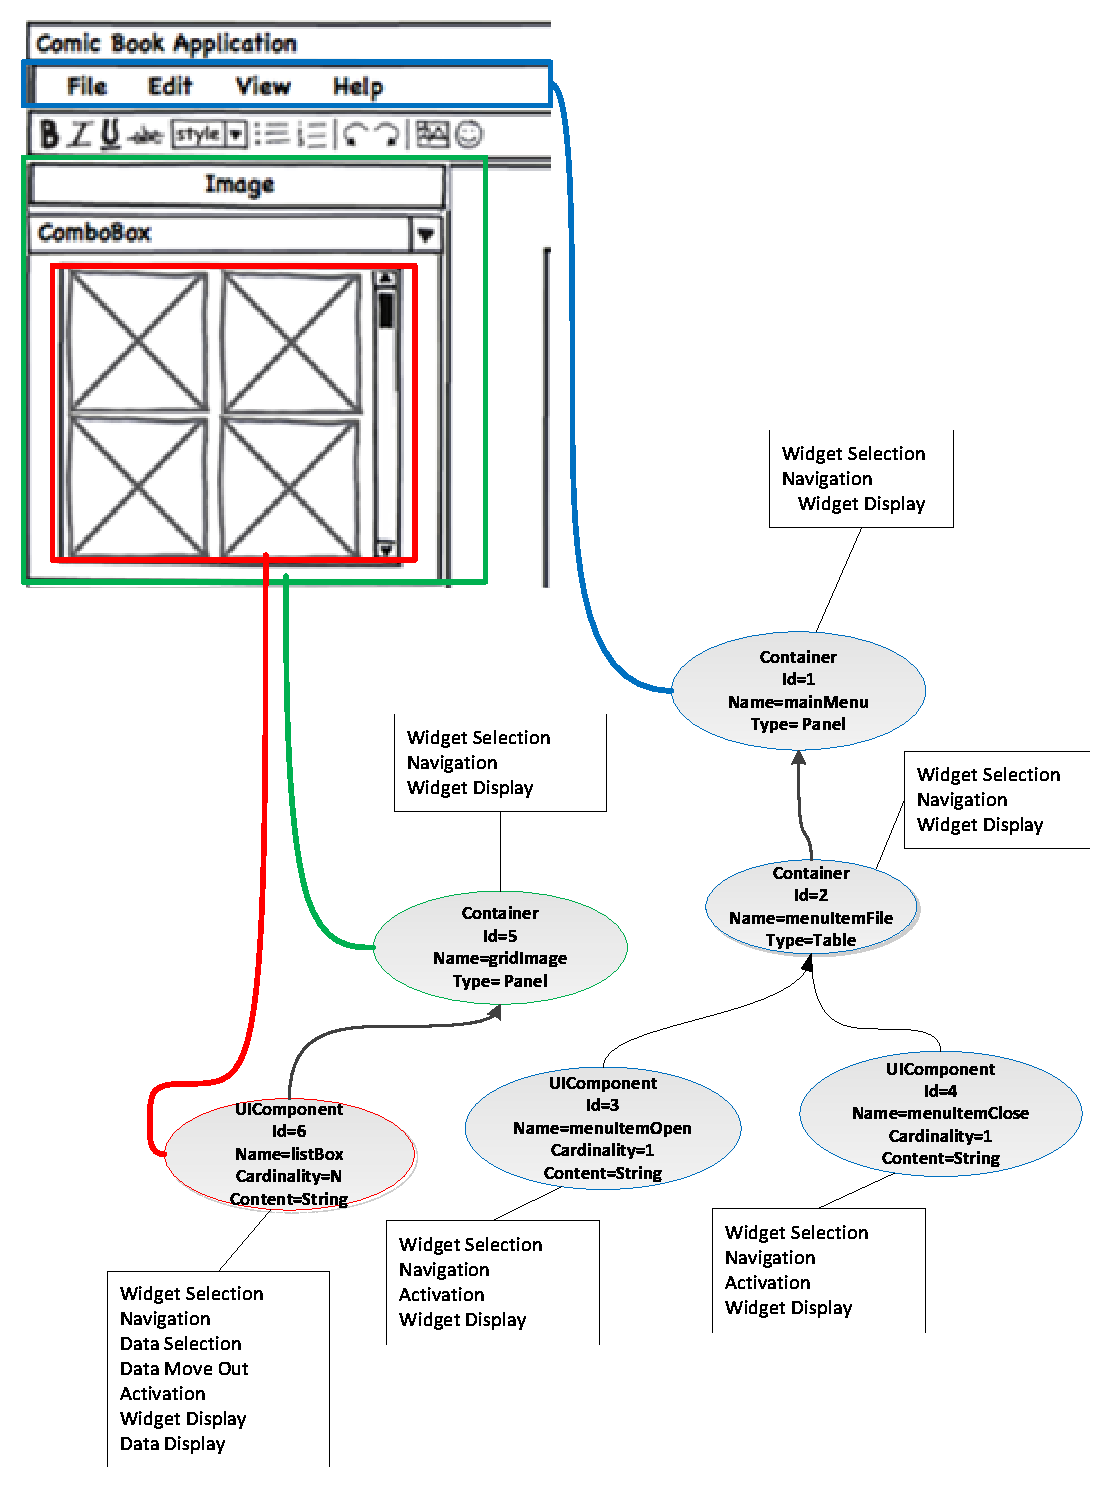
\includegraphics[width=0.7\linewidth]{chap4/image6}
\caption{Art�fact d'UI}
\label{fig:image6}	
\end{figure}
\end{center}


Pour chaque interacteur correspondant aux Widgets d�crits ci-dessus,
nous appliquons l'algorithme d�crit � la section 6.2.2.1 pour rechercher les
widgets �quivalents dans la biblioth�que graphique XAML Surface (cf. annexe). Le
tableau des widgets �quivalents obtenu correspond au tableau. Ce tableau nous
montre que~:

\begin{enumerate}
\item  le container \textit{gridImage} est strictement �quivalent �
\textit{Grid}, le \textit{Widget} \textit{ScatterViewItem} a en plus les
primitives d'interaction \textbf{Widget Move} et \textbf{Widget Resize}.
L'op�rateur \textbf{\textit{simpleEquivalent}} ne trouve rien de plus que
l'op�rateur \textbf{\textit{largeEquivalent}} car l'interacteur de d�part
(\textit{gridImage}) ne contient pas de donn�es~; par cons�quent il n'a pas de
type de donn�e. L'op�rateur \textbf{\textit{lowEquivalent}} ne trouve rien car
les autres colonnes du tableau ne sont pas vides. 

\item  L'interacteur \textit{listBox} n'a pas de Widget strictement �quivalent
dans la biblioth�que XAML Surface car il n'impl�mente pas la primitive
d'interaction \textbf{Data Move In}  qui est intrins�que � une \textit{ListBox}.
L'op�rateur \textbf{\textit{largeEquivalent}} retrouve \textit{SurfaceListBox}
car il d�crit des primitives d'interactions en plus. L'op�rateur
simpleEquivalent permet de retrouver des widgets qui supportent d'autres types
de donn�es. L'op�rateur \textbf{\textit{lowEquivalent}} ne trouve rien car les
autres colonnes du tableau ne sont pas vides.

\item  Le container contenant les �l�ments du menu principal (\textit{mainMenu})
est strictement �quivalent � un \textit{Grid}, il a une �quivalence large avec
un \textit{ScatterViewItem} (qui impl�mente les primitives d'interaction
\textbf{Widget Move} et \textbf{Widget Resize} en plus), et n'as pas de widgets
�quivalent simplement ou d'une �quivalence faible. Le choix du
\textit{ScatterViewItem} permettra d'avoir un menu d�pla�able et utilisable
partout sur la table interactive. L'op�rateur \textbf{\textit{lowEquivalent}} ne
trouve rien car les autres colonnes du tableau ne sont pas vides.

\item  Les �l�ments du menu (\textit{menuItemFile, menuItemEdit}) ont des
widgets �quivalents suivants les op�rateurs d'�quivalence stricte, large ou
simple. L'op�rateur \textbf{\textit{lowEquivalent}} ne trouve rien car les
autres colonnes du tableau ne sont pas vides.
\end{enumerate}
\begin{table} %{|p{1.1in}|p{0.9in}|p{0.9in}|p{0.8in}|p{0.3in}|}
\begin{tabularx}{15cm}{|Y|Y|Y|Y|p{0.3in}|} 
\hline  \textbf{Interactor Id/Name} 
		& \textbf{Strong} 
		& \textbf{Large} 
		& \textbf{Simple}
		& \textbf{Low} \\ 
\hline Id=5, Name=gridImage 
		& Grid 
		& ScatterViewItem 
		&  
		&  \\ 
\hline Id=6, Name=listBox 
		&  
		& SurfaceListBox 
		& LibraryContainer, LibraryBar 
		&  \\ 
\hline Id=1, Name=mainMenu 
		& Grid 
		& ScatterViewItem 
		&  
		&  \\ 
\hline Id=2, Name=menuItemFile 
		& ElementMenu, Grid 
		& ScatterViewItem 
		& LibraryContainer, LibraryBar 
		&  \\ 
\hline Id=3, Name=menuItemOpen 
		& ElementMenuItem, Button 
		&  
		& Image 
		&  \\
\hline Id=4, Name=menuItemClose 
		& ElementMenuItem, Button 
		&  
		& Image 
		& \\ 
\hline 
\end{tabularx}
\caption {Equivalent Widget}
\label{tab:chap5:1}
\end{table}
L'algorithme de s�lection permet d'avoir l'ensemble des widgets
�quivalents pour un interacteur donn� dans le tableau des widgets �quivalents.
L'utilisation des �l�ments de cet ensemble pour la migration est guid�e par les
guidelines de la plateforme d'arriv�e qui permettra d'abord de classer les
widgets �quivalents, ensuite de proposer une version d'UI migr�e et enfin pour
faciliter la personnalisation de cette proposition.


\subsection{Classement des widgets}

Le processus de classement des widgets � pour but d'assister les
d�veloppeurs dans le choix des widgets de la plateforme d'arriv�e. Ce processus
d�termine les `\textit{meilleurs widgets'} de la classe d'�quivalence d'un
interacteur � l'aide d'une fonction qui prend en compte deux crit�res~: les
principes du guidelines et la charge de travail pour le programmeur. Cette
fonction permet de consid�rer le classement des widgets �quivalents � un
interacteur comme une instance d'un probl�me d'optimisation qui consiste �
trouver les widgets qui sont conformes aux principes des guidelines (maximiser
les crit�res conformes aux guidelines) et qui r�duit la charge de travail pour
le d�veloppeur (minimiser la charge de travail). 

Cette section d�crit la prise en compte des guidelines (6.3.1) et la
charge de travail pour le programmeur (6.3.2) comme crit�re pour le classement
des widgets utilis�e par l'algorithme de classement (6.3.3).


\subsubsection{Prise en compte des guidelines}

La prise en compte des guidelines se fait en se basant sur les
primitives d'interactions intrins�ques et les types de donn�es qui caract�risent
les widgets de mani�re ind�pendante des biblioth�ques graphiques. Elle se fait
d'abord en traduisant ses principes sous formes de r�gles appliqu�es sur les
caract�ristiques des composants graphiques dans le but de les classer. Ensuite
en calculant la conformit� de chaque widgets aux principes des guidelines
formalis�es en r�gles.


\subsubsection{Traduction des principes du guidelines en r�gles de classement des widgets �quivalents.}

Les principes des guidelines � consid�rer par le processus de
classement sont celles qui facilitent le choix des widgets �quivalents. En
consid�rant les 2 premiers principes d�crits par le chapitre 4~:

\begin{enumerate}
\item  \textbf{G1}:\textit{``Provide a 360-Degree User Interface''}

\item  \textbf{G2}\textit{:`` Make Experiences Natural and Better than Real''} 
\end{enumerate}

La traduction de ces deux principes pour le processus de classement
des widgets �quivalents conform�ment aux deux �tapes pr�sent�s  � la section
\eqref{GrindEQ__4_3_5_} se fait en identifiant les �l�ments de l'UI qui
permettront de faciliter le choix des widgets ensuite nous pr�ciseront comment
ces �l�ments faciliterons le classement des widgets �quivalents.

\textbf{G1} s'applique sur les primitives d'interactions car en
privil�giant les widgets qui ont des primitives d'interactions interaction
\textbf{Widget Move }et \textbf{Widget Rotation,} tous les utilisateurs auront
aux widgets qui l'ont ind�pendamment de leur orientation ou de leur position
autour de la table interactive. 

\textbf{R�gle 1}: Les primitives d'interaction \textbf{Widget Move }et
\textbf{Widget Rotation} sont privil�gi�s pour les containers.

\textbf{G2}  s'applique sur les types des donn�es car le choix des
widgets ayant des types de donn�es  images, son ou vid�o permet de r�v�ler leur
contenu � l'utilisateur. 

\textbf{R�gle 2}: Les types \textbf{Image}, \textbf{MediaElement et
Object} sont mieux consid�r�s pour widgets ayant des contenus sur une table
interactive.

Ces deux r�gles pr�cisent les �l�ments du mod�le des primitives
d'interaction sur les quels peuvent s'appliquer les guidelines G1 et G2 des
guidelines de la table interactive. La conformit� par rapport � ces r�gles est
d�termin�e par les fonctions d�crites ci-dessous.


\subsubsection{Conformit� des widgets aux principes du guideline}

Pour marquer l'importance de certaines caract�ristiques (primitives
d'interaction et type de donn�es) par rapport � d'autres, un poids est attribu�
� celles qui sont conforme aux principes du guidelines. Le choix de la valeur du
poids se fait par le programmeur avant la migration et ce choix permet de
d�terminer s'il pr�f�re maximiser la conformit� aux principes du guidelines par
rapport � la charge de travail ou s'il pr�f�re l'inverse. 

L'ensemble des poids des primitives d'interactions d'un Widget est
d�termin� par la fonction$\ {\mathbf Interactions}{\mathbf Weight}{\mathbf
:}{\mathbf Widget}\to {\mathbf \ }\left\{Interger\right\}{\mathbf \ }$ en
utilisant le tableau ci-dessous.

L'ensemble des poids des types des donn�es d'un Widget est d�termin�
par la fonction ${\mathbf DataType}{\mathbf Weight}{\mathbf :}{\mathbf
Widget}\to {\mathbf \ }\left\{Interger\right\}$ en utilisant le tableau
ci-dessous.

Ce tableau pr�cise un poids non nul pour  les primitives
d'interactions et les types de donn�es conformes aux R�gle 1 et 2 ci-dessus. 

\begin{tabular}{|p{1.9in}|p{1.5in}|p{0.3in}|} \hline 
\textbf{Primitive d'interaction} & \textbf{Type de donn�es} & \textbf{Poids} \\
\hline 
Widget Move, Widget Rotation & Image, M�dialement, Object & P$>$0 \\ \hline 
Toutes les autres primitives d'interaction  & Tous les autres types de donn�es &
0 \\ \hline 
\end{tabular}



Nous formalisons le calcul de la conformit� d'un Widget aux principes
des guidelines par la fonction$\ {\mathbf guidelinesRate}{\mathbf :}Widget\to
Integer$. Cette fonction est la somme des fonctions repr�sentant les
caract�ristiques  suivantes prises en compte pour d�terminer la conformit� aux
principes des guidelines~:

\begin{enumerate}
\item  la prise en compte des primitives d'interaction se fait par la
fonction${\mathbf \ }{\mathbf interactionRate}{\mathbf :}Widget\to Integer$,
elle permet de faire la somme des poids des primitives d'interaction
intrins�ques qui sont conformes aux principes des guidelines. Les widgets
�quivalents � un interacteur sont identifi�s par le processus dans la table
\textbf{\textit{EquivalentWidget}}.
\[\ \forall w\in {\mathbf EquivalentWidget},\ \ {\mathbf
interactionRate}\left({\mathbf w}\right){\mathbf =}\sum{{{\mathbf P}}_{{\mathbf
i}}}{\mathbf ,\ }{{\mathbf P}}_{{\mathbf i}}\in {\mathbf Interactions}{\mathbf
Weight}{\mathbf (}w{\mathbf )}\] 

\item  La prise en compte des types de donn�es est effectu�e par la fonction$\
{\mathbf dataTypeRate}{\mathbf :}Widget\to Integer$, cette fonction fait la
somme des poids des types de donn�es des widgets �quivalents � un interacteur.
\[\forall w\in {\mathbf EquivalentWidget},\ \ {\mathbf
dataTypeRate}\left({\mathbf w}\right){\mathbf =}\sum{{{\mathbf P}}_{{\mathbf
i}}}{\mathbf ,\ }{{\mathbf P}}_{{\mathbf i}}\in {\mathbf DataType}{\mathbf
Weight}{\mathbf (}w{\mathbf )}\] 
\end{enumerate}
La fonction ${\mathbf guidelinesRate}\left(w_{{\mathbf i}}\right){\mathbf
=}{\mathbf interactionRate}\left(w_i\right){\mathbf +\ }{\mathbf
dataTypeRate}{\mathbf (}w_i{\mathbf )}$\textbf{ }pour tout $w_{{\mathbf
i}}$\textbf{ }appartenant � la classe des widgets �quivalents � un interacteur.


\subsection{Charge de travail du programmeur}

Le choix d'un Widget conforme aux principes des guidelines peut
entrainer soit l'ajout d'un connecteur pour l'adaptation de type de donn�es,
soit l'ajout des nouvelles donn�es pour l'interface utilisateur , soit l'ajout
de codes suppl�mentaires pour la prise en compte des nouvelles primitives
d'interactions. L'ajout d'un connecteur [Mehta, Medvidovic, and Phadke 2000]
consiste � g�n�rer un code qui permet de faire un changement de type entre le
type de donn�es de l'interacteur et le type de donn�es support� par les widgets
�quivalents, cette t�che est automatisable pour l'ensemble des types de donn�es
d'une biblioth�que graphique, elle n'entraine pas  une charge de travail pour le
programmeur.

Cependant, l'ajout des donn�es suppl�mentaires engendr� par le choix
d'un Widget n'est pas automatisable car l'utilisateur doit trouver ou cr�er ces
donn�es et ensuite faire le `\textit{mapping'} avec les types de donn�es d�part.
Par exemple le remplacement d'un menu classique dont les �tiquettes sont des
chaines de caract�res avec un menu dont les �tiquettes sont des icones (Images)
n�cessite la recherche ou la cr�ation de ces ic�nes. 

Par ailleurs, l'ajout de code suppl�mentaire pour la prise en compte
des nouvelles primitives d'interaction est une t�che manuelle car les codes �
ajouter d�pendent des primitives d'interactions intrins�ques � impl�ment�es.


\subsubsection{Calcule de la charge de travail}

Les crit�res permettant le calcul de la charge de travail engendr�e
par le choix d'un Widget sont~: la diff�rence entre le type de donn�es de
l'interacteur et celui des widgets �quivalent, et les primitives d'interaction
intrins�ques en plus des widgets �quivalents. A chacun de ces crit�res, le
programmeur associe un co�t en se basant sur ses comp�tences pour r�aliser une
t�che. L'estimation de ce co�t peut se faire en se basant sur la technique
\textit{Pomodoro} [Gobbo and Vaccari 2008] qui est utilis�e en \textit{Extreme
Programming} [Beck 2000] pour permettre aux programmeurs d'optimiser leur temps
de programmation en �valuant au mieux le temps de diff�rentes t�ches �
effectuer.

La fonction$\ {\mathbf workLoad}{\mathbf :}{\mathbf
Interactor}{\mathbf \times }{\mathbf Widget}\to {\mathbf I}??{\mathbf
teger}$\textbf{, }calcule la charge de travail engendr�e par le choix d'un
widget �quivalent � un interacteur. C'est une somme des co�ts de chaque crit�re
v�rifi� par le widget � choisir. Les crit�res sont~:

\begin{enumerate}
\item  la n�cessit� des donn�es suppl�mentaires � la suite d'un changement de
type. Ce crit�re est v�rifi� si l'interacteur et le widget � choisir n'ont pas
le m�me type de donn�es et si le type de donn�es du widget est \textbf{Image},
\textbf{MediaElement }ou \textbf{Object.~}Le co�t de ce crit�re est donn� par la
fonction${\mathbf \ }{\mathbf DataTypeCost}~{\mathbf :\ }{\mathbf
Interactor}{\mathbf \times }{\mathbf Widget}\to {\mathbf Integer}$ � l'aide du
tableau ci-dessous qui permet aussi au programmeur de pr�ciser avant la
migration le co�t de chaque op�tation.

\item  L'utilisation des primitives d'interactions intrins�ques des widgets
�quivalent. Ce crit�re est calcul� par la fonction${\mathbf \ }{\mathbf
InteractionCost}{\mathbf :}{\mathbf Interactor}{\mathbf \times }{\mathbf
Widget}\to {\mathbf Integer}$ en utilisant le tableau ci-dessous. 
\end{enumerate}

Dans ce tableau, le co�t de chaque t�che manuelle est estim� par le
programmeur avant de commencer une migration. De nouvelles op�rations manuelles
peuvent �tre d�finies, cette liste n'est pas exhaustive.

\begin{tabular}{|p{2.4in}|p{1.6in}|} \hline 
\textbf{Operations Manuelles} & \textbf{Co�t estim� par le programmeur} \\
\hline 
Nouvelles ressources de type Image  & C${}_{1}$$>$0 \\ \hline 
Nouvelles ressources de type Media Element & C${}_{2}$$>$0 \\ \hline 
Nouvelles ressources de type Object & C${}_{3}$$>$0 \\ \hline 
Code de redimensionnement des widgets d'un container & C${}_{2}$$>$0 \\ \hline 
Code permettant de faire un Drop & C${}_{4}$$>$0 \\ \hline 
Code permettant de faire un Drag & C${}_{5}$$>$0 \\ \hline 
\end{tabular}

La charge de travail est calcul�e par la fonction~:
\[{\mathbf workLoad}\left({\mathbf interactor}{\mathbf ,\ }{\mathbf
widget}\right){\mathbf =\ }\sum{{{\mathbf C}}_{{\mathbf i}}}{\mathbf ,\ \
}{{\mathbf C}}_{{\mathbf i}}\in {\mathbf DataTypeCost}\left({\mathbf
interactor},{\mathbf widget}\right)\cup {\mathbf InteractionCost}\left({\mathbf
interactor},{\mathbf widget}\right)\] 


\subsection{Algorithme de classement }

L'algorithme de classement d�termine le rang de chaque widget de la
classe d'�quivalence d'un interacteur en faisant la diff�rence entre la
conformit� aux guidelines et le charge de travail. La fonction$\ F:{\mathbf
Interactor}{\mathbf \times }{\mathbf Widget}\to {\mathbf Integer}{\mathbf \
}$d�termine la valeur de l'objectif d'un widget appartenant � une classe
d'�quivalence. Cette valeur permet de classer le widget dans la classe
d'�quivalence de l'interacteur.$\ \forall \ i\in \left\{Interactor\right\},\
\forall w\in {\mathbf EquivalentWidget}\left({\mathbf i}\right),$\textbf{ }
\[{\mathbf F}{\mathbf (}{\mathbf i},{\mathbf w}{\mathbf )=}{\mathbf
gu}??{\mathbf delinesRate}\left({\mathbf w}\right){\mathbf -}{\mathbf
workLoad}{\mathbf (}{\mathbf i},{\mathbf w}{\mathbf )}.\] 
Le `\textit{meilleurs widget'} en consid�rant les principes du guidelines est
celui qui a le max de la fonction$\ {\mathbf F};;$
\[{\mathbf BestEquivalentWidget}\left({\mathbf i}{\mathbf ,\ }{\mathbf
EquivalentWidget}\right){\mathbf =}max\left(\bigcup_{\forall \ w\in {\mathbf
EquivalentWidget}\left(i\right)}{\left({\mathbf F}{\mathbf (}{\mathbf
i},{\mathbf w}\right)}\right)\ .\] 


\subsubsection{Exemple de classement}

Consid�rons les interacteurs \textit{id=6} et \textit{id=1} de
l'exemple d�crit � la section 6.2.2.2 et les widgets de leurs classes
d'�quivalence. 

Consid�rons que le programmeur souhaite utilis�s les widgets les plus
conformes aux principes des guidelines et pour cela fixe la valeur du poids des
primitives d'interactions � P=2 et les co�ts C${}_{i }$=1, 0$<$i$<$6

 Le widget \textit{SurfaceListBox} de la classe d'�quivalence de
l'interacteur id=6 a pour type de donn�es \textit{String.} 
\[guidelines\left(offSurfaceListBox\right)=interactionRate\left(SurfaceListBox\right)+dataType\left(SurfaceListBox\right)=0+0=0\]

\[\ workload\left(listBox,SurfaceListBox\right)=0+0+0+0+0\] 
\[F\ (listBox,\
SurfaceListBox)=guidelines\left(offSurfaceListBox\right)-workload\left(listBox,SurfaceLi??tBox\right)=0-0=0\]

%\begin{flushleft}
% Les widgets \textit{LibraryContainer }et\textit{ LibraryBar} ont pour type de
%donn�es \textit{Object}.
%\[guidelines\left(offLibraryContainer\
%\right)=interactionRate\left(LibraryContainer\
%\right)+dataType\left(LibraryContain??r\ \right)=0+2=2\] 
%\[\ workload\left(listBox,SurfaceListBox\right)=0+0+1+0+0\] 
%\[F\ (listBox,\
%SurfaceListBox)=guidelines\left(offSurfaceListBox\right)-workload\left(listBox,SurfaceListBox\right)=2-1=1\]
%
%Le widget ScatterView a en plus les primitives d'interactions Widget Rotation et
%Widget Move.
%\[guidelines\left(offScatterView{\rm \
%}\right)=interactionRate\left(ScatterView{\rm \
%}\right)+dataType\left(ScatterView{\rm \ }\right)=4+0=4\] 
%\[\ workload\left(main??enu,ScatterView{\rm \ }\right)=0+0+0+0+0\] 
%\[F\ (mainMenu,\ ScatterView{\rm \ })=guidelines\left(offScatterView{\rm \
%}\right)-workload\left(mainMenu,ScatterView{\rm \ }\right)=4-0=4\] 
%Le widget Grid n'a pas de primitives d'interactions en plus ou  des type de
%donn�es diff�rents
%\[guidelines\left(offGrid{\rm \ }\right)=interactionRate\left(Grid{\rm \
%}\right)+dataType\left(Grid{\rm \ }\right)=0+0=0\] 
%\[\ workload\left(mainMenu,Grid{\rm \ }\right)=0+0+0+0+0\] 
%\[F\ (mainMenu,\ Grid{\rm \ })=guidelines\left(offGrid{\rm \
%}\right)-workload\left(mainMenu,Grid{\rm \ }\right)=0-0=0\] 
%\end{flushleft}
%
%\begin{tabular}{|p{0.7in}|p{0.8in}|p{1.7in}|p{0.3in}|} \hline 
%\textbf{Interacteur\newline Id/ Name} & \textbf{Widget \newline Equivalent} &
%${\mathbf F}\left({\mathbf i},{\mathbf w}\right){\mathbf =}$\textbf{\newline
%}${\mathbf guidelinesRate}\left({\mathbf w}\right){\mathbf -}{\mathbf
%workLoad}{\mathbf (}{\mathbf i},{\mathbf w}{\mathbf )}$ & \textbf{Rang}
%\\ \hline 
%Id=6\newline Name=listBox & SurfaceListBox & 0 & 3 \\ \hline 
% & LibraryContainer & 1 & 1${}^{*}$ \\ \hline 
% & LibraryBar & 1 & 1${}^{*}$ \\ \hline 
%Id=1\newline Name=mainMenu & Grid & 0 & 0 \\ \hline 
% & ScatterView & 4 & 1${}^{*}$ \\ \hline 
%\end{tabular}
%
%\begin{flushleft}
%\textit{${}^{*}$Les `meilleurs' widgets}
%\end{flushleft}
%
Le classement des widgets �quivalents facilite leur choix pour la
prochaine �tape du processus de migration. Cette �tape consiste � proposer � aux
concepteurs une  premi�re version d'UI pour la table interactive. La mise en
?uvre de cette premi�re version se fait utilisant le classement propos� � cette
�tape et en consid�rant les principes des guidelines relatives � la structure de
l'UI et aux interactions. 


\section{Personnalisation de l'UI propos�e}

La personnalisation de l'UI migr�e sur la table interactive � pour
objectifs de produire une UI finale conforme aux attentes des concepteurs et qui
respecte les crit�res ergonomiques li�s aux tables interactives. Cette �tape
fait intervenir les concepteurs pour modifier et fa�onner la structure, les
interactions et l'aspect visuel de l'UI g�n�rer automatiquement � la phase
pr�c�dente. Le processus de personnalisation assiste les concepteurs pour chaque
action de modification de l'UI propos�e. Cette section pr�sente les diff�rentes
actions des concepteurs et l'assistance apport�e par le processus � l'aide des
guidelines.


\subsection{Op�rations de modification de la structure}

La personnalisation de la structure d'UI propos�e permet aux
concepteurs de remplacer, repositionner, redimensionner les composants
graphiques\textit{.} Elle permet aussi d'effectuer les op�rations manuelles
d�crite � la section 6.3.2.1 telles que l'ajout de nouvelles ressources d'UI,
l'ajout de code par exemple. Cette �tape permet enfin l'�dition des aspects
visuels de l'UI (couleurs, taille, police, etc.) gr�ce � un �diteur graphique.
Les op�rations manuelles de personnalisation de l'UI sont �valu�es par rapport �
leurs conformit�s aux des guidelines de la table interactive. 


\subsubsection{Remplacer des composants}

Cette op�ration permet de changer un ou plusieurs composants
graphiques choisis pendant la phase pr�c�dente. Cette op�ration utilise les
r�gles de classements des widgets �quivalents pour �valuer la conformit� aux
guidelines (G1 et G2) et la charge de travail. 


\subsubsection{Supprimer un composant graphique}

Cette op�ration permet de r�duire les composants graphiques dans le
but de bloquer l'acc�s � des fonctionnalit�s non d�sir�es par l'utilisateur sur
la table interactive. La guideline G19 justifie cette op�ration car elle
pr�conise la r�duction des fonctionnalit�s~; le choix des fonctionnalit�s �
conserver d�pend des applications � migrer et des objectifs de concepteur. Les
composants graphiques supprim�s dans la structure \textit{TargetUIStructure}
sont aussi supprim�s dans le mod�le de structure \textit{TargetAUIStructure.}

L'assistance permet � l'utilisateur de v�rifier si deux interacteurs
activent la m�me m�thode du contr�leur. En effet les primitives d'interactions
effectives du mod�le \textit{TargetAUIStructure} permettent  de retrouver
l'ensemble des interacteurs qui permettent d'activer la m�me m�thode du
Contr�leur. La  ${\mathbf findInterac}??{\mathbf orByMethods}$\textbf{
}ci-dessous est utilis�e par les concepteurs avant la suppression d'un composant
graphique pour retrouver les composants graphiques activants les m�mes
fonctionnalit�s.
%\[{\mathbf findInteractorByMethods}:MethodSignature\times TargetAUIStructure\to
%\ \left\{Interactor\right\}\] 
%\[\forall \ interactor\in TargetAUIStructure\wedge \exists \ activation\in
%interactor.getEffectiveInteraction\left(off\right)\wedge
%typeOf\left(activation\right)={\mathbf Activation}\] 
%\textbf{Si}$\ \left( \begin{array}{c}
%\exists interactor \in TargetAUIStructure\wedge interactor  \ne interactor  \\
%
%\wedge \exists \ activation  \in interactor .getEffectiveInteraction() \\ 
%\wedge typeOf \left(activation  \right)={\mathbf Activation} \\ 
%\wedge \exists methodSignture\in activation.inputMethods \\ 
%\wedge methodSignture\in activation'.inputMethods \end{array}
%\right)$ 
%
%\textbf{Alors}${\mathbf \ }interactor \in {\mathbf
%findInteractorByMethods}\left(methodSignture,TargetAUIStructure\right)$


\subsubsection{Dupliquer un groupe de composants graphiques}

Cette op�ration � pour objectifs multiplier les composants graphiques
pour permettre � tous les utilisateurs autour de la table d'y avoir acc�s
facilement. Elle est pr�conis�e par les guidelines G7, G8 et G18. La duplication
concerne les containers de type \textit{Panel} ou \textit{Table} et leurs fils
car ils peuvent �tre concr�tis�s comme des menus, ou des groupes permettant la
consultation des contenus. Les composants graphiques dupliqu�s dans la structure
\textit{TargetUIStructure} sont aussi dupliqu�s dans le mod�le de structure
\textit{TargetAUIStructure.}

L'assistance pour la duplication permet aux concepteurs de
s�lectionner les interacteurs repr�sentant des menus ou des contenus �
dupliquer.

\begin{enumerate}
\item  Les menus sont d�crits � l'aide des \textit{Container} de type Table et
qui contiennent des \textit{UIComponent} ayant que les primitives d'interactions
effectives de cet ensemble $\left\{Widget\ Selection,\ \ Navigation,\
Activation,\ WidgetDisplay\right\}$ 

\item  Les groupes de composant permettant la consultation des contenus sont
d�crits � l'aides des \textit{Container} de type Table ou Panel qui contiennent
des \textit{UIComponent} avec des contenu ($UIComponent.Content!=Null$) et
n'ayant les primitives d'interaction effective$\ Data\ Edition\ et\ Activation$.
\end{enumerate}


\subsubsection{Op�rations de personnalisation des interactions}

Cette cat�gorie regroupe les op�rations qui permettent de d�finir
l'utilisation des dispositifs d'interactions et les op�rations manuelles
impos�es par le choix des widgets �quivalents. 


\subsubsection{Associer un objet physique � un groupe de widgets }

Cette op�ration permet l'utilisation des objets tangibles comme moyens
d'interaction pour afficher des composants graphiques ou pour activer. En effet
les recommandations des guidelines G15 et G16 permet d'utiliser les objets
physiques pour afficher un menu ou un formulaire. Elle concerne que les
\textit{Container} de type \textit{Table} et de type \textit{Panel.}


\subsubsection{Compl�ter les codes }

\begin{flushleft}
Cette op�ration permet aux concepteurs de compl�ter les codes non g�n�rer
automatiquement � la phase de g�n�ration de \textit{TargetUIStructure}.
\end{flushleft}


\subsection{Op�rations de personnalisation de l'aspect visuelle de l'UI}

L'ensemble des op�rations de personnalisation de l'aspect visuelle de
l'UI pour permettre une utilisation naturelle de l'UI. 


\subsubsection{D�finir un layout}

Cette op�ration permet de placer  les �l�ments d'un \textit{Container}
de type \textit{Panel} car ils sont empil�s ou dispos�s al�atoirement en
fonction du l'impl�mentation du g�n�rateur de l'UI propos�e. Le concepteur doit
d�finir le layout de chaque container de type \textit{Panel} manuellement. Elle
est conforme � la guideline G40 qui pr�conise de structurer les widgets d'un
container qui est conforme � G1.


\subsubsection{Ajouter les ressources de l'UI}

Cette op�ration permet aux concepteurs d'ajouter des ic�nes, des
images ou d'autres ressources pour permettre une utilisation naturelle de l'UI,
elle s'inspire de G4 qui pr�conise l'utilisation des composants graphiques ayant
des contenus qui facilitent l'interaction.


\subsubsection{D�finir le style de textes et les couleurs}

Ces op�rations permettent la personnalisation des textes descriptifs
(�tiquettes, info-bulles, etc.). Elles sont  d'�tre conformes aux guidelines
G34, G35, G36, G45, G46, G47, G48, G50, G51.


\subsection{Synchronisation du mod�le  TargetAUIStructure et TargetUIStructure}

Les op�rations d�crites ci-dessus sont effectu�es par le concepteur
sur l'UI permettent  d'abord de modifier \textit{TargetUIStructure, }cependant
les op�rations de personnalisation de la structure ont ensuite un impacte sur le
mod�le de structure\textit{ TargetAUIStructure.} La synchronisation du mod�le et
sa concr�tisation permettent de garder une coh�rence pour les op�rations de
modifications suivantes.


\section{Synth�se }
	%
	\chapter{M�canismes de migration des UI}
	%\label{chap6}
	%\minitoc
	%\section{Introduction}
\label{sec:chap6:1}

Le processus de migration que nous proposons est bas� sur les primitives d'interactions\footnote{Elles constituent aussi  un mod�le d'interactions abstraites} et un mod�le de structure de l'UI. Conform�ment aux approches bas�es sur les mod�les~\cite{Moore1997,Paterno'2009} �tudi�es au chapitre~\ref{chap3}, notre processus de migration comporte trois grande phases: \begin{itemize}
\item la premi�re consiste � d�crire l'application � migrer � l'aide des mod�les abstraits par un processus d'abstraction.
\item La deuxi�me phase consiste � transformer le mod�le de structure l'application de d�part pour la plateforme cible tout en prenant en compte les guidelines et en pr�servant au moins les interactions de d�part. Les interacteurs de la structure de l'UI transform�e sont des instances des composants graphiques de la plateforme cible. L'identification de ces interacteurs ce fait en \textbf{comparant les primitives d'interactions} effectives des interacteurs de l'UI source avec les primitives d'interactions des composants graphiques instanci�s de la plateforme cible.
\item La troisi�me consiste � produire l'UI finale de la plateforme cible en int�grant les aspects (style et layout)  qui ne sont pas pris en compte par les mod�les abstraits. La g�n�ration de l'UI finale consiste d'une part � s�lectionner pour chaque interacteur \textbf{le composant graphique �quivalent} conform�ment aux guidelines, d'autre part les composants s�lectionn�s sont positionn�s manuellement suivant les guidelines associ�es � la plateforme cible.
\end{itemize}

Les deux derni�re phase de ce processus de migration font appels � la \textbf{comparaison entre les interacteurs} en se basant sur les primitives d'interactions et la \textbf{s�lection de composant graphique} en fonction des primitives d'interactions. Ces deux notions d�finissent des �quivalences en se basant sur les primitives d'interactions entre les interacteurs des structures des UI sources et cibles d'une part et entre les interacteurs de l'UI cible et les composants graphiques de la plateforme cible d'autre part. 

Cette section se propose de d�finir et formaliser les op�rateurs de comparaison entre les interacteurs et les composants en se basant sur les primitives d'interactions.

	
	\chapter{Validations du processus}
	%\label{chap7}
	%\minitoc
	%\section{Introduction}
\label{sec:chap7:1}
Les syst�mes interactifs (SI) � migrer peuvent avoir une d�composition fonctionnelle minimale de la figure %\ref{fig:chap3:1} 
qui comprend une interface utilisateur (UI) et un noyau fonctionnel (NF). La migration des SI vers la table interactive est un processus qui impacte � la fois le NF et l'UI. 


\subsection{Introduction}
La solution de migration assist\'{e}e que nous proposons est constitu\'{e}e 
de trois phase~: la phase d'extraction \`{a} partir de la structure 
analysable ({\it UIStruture}) d'une repr\'{e}sentation ({\it AUIStructure}) qui est d\'{e}crite dans le 
chapitre pr\'{e}c\'{e}dent, la phase d'adaptation de la structure de l'UI 
aux r\`{e}gles ergonomiques de la table interactive et enfin la phase de 
projection du mod\`{e}le d'UI adapt\'{e}, cette phase permet aussi aux 
concepteurs de personnaliser l'UI finale. 

\subsection{Adaptation de la structure de l'UI }
\label{subsec:adaptation}
Cette phase a pour finalit\'{e} la production d'une structure d'UI 
adapt\'{e}e aux r\`{e}gles ergonomiques de la table interactive. 
L'adaptation du mod\`{e}le de structure ({\it AUIStructure}) extraite de l'UI \`{a} migrer se 
fait en fonction des r\`{e}gles ergonomiques que nous pr\'{e}sentons \`{a} 
la section \ref{subsubsec:mylabel1}. La section 
\ref{subsubsec:identification} pr\'{e}sente une formalisation des r\`{e}gles 
d'adaptation de la structure et enfin la section 
\ref{subsubsec:mylabel2} est une synth\`{e}se du processus 
d'adaptation de la structure.

\subsubsection{R\`{e}gles ergonomiques pour l'adaptation du mod\`{e}le AUIStructure}
\label{subsubsec:mylabel1}
\paragraph{R\`{e}gles ergonomique pour l'adaptation des groupes d'interacteurs}
Les guidelines G1, G38, G39 et G40 sont rattach\'{e}es de G18 qui 
pr\'{e}conise de prendre en compte le nombre d'utilisateur et le partage de 
l'\'{e}cran pendant la mise en \oe uvre de l'UI. En effet ce principe impact 
la structuration des groupes d'interacteurs (G38, G38, G40) en fonction de 
leur contenu, elle impacte aussi l'accessibilit\'{e} de ces groupes qui 
doivent \^{e}tre 360\textdegree utilisable (G1). Les r\`{e}gles 
d'adaptations relatives \`{a} ces principes doivent consid\'{e}rer les types 
de Container ({\it Window, Simple, Panel }et{\it Table}). 

\paragraph{Guidelines d'utilisation des objets tangibles}
Les guidelines G15, G16 et G18 sont rattach\'{e}es \`{a} G5 pr\'{e}conise la 
consid\'{e}ration des objets physiques comme moyen d'interaction. Elles 
pr\'{e}cisent les cadres d'utilisation des objets tagu\'{e}s ou non. Les 
r\`{e}gles associ\'{e}es \`{a} ces guidelines ne sont pas appliqu\'{e}es 
dans tous les pendant cet \'{e}tape du processus, le concepteur doit 
pr\'{e}ciser dans s'il souhaite les appliquer avant la g\'{e}n\'{e}ration de 
l'UI propos\'{e}e.

\subsubsection{Identification des r\`{e}gles d'adaptation}
\label{subsubsec:identification}
Les r\`{e}gles identifi\'{e}es dans cette section permettent de 
g\'{e}n\'{e}rer la structure de l'UI pour la table interactive, cette 
structure est d\'{e}crite par l'ensemble $TargetUIStructure$ \`{a} l'aide 
des widgets de la plateforme cible.

\paragraph{R\`{e}gles d'adaptation des containers de type Table}
Les containers de type {\it Table} sont compos\'{e}s des {\it UIComponent} ayant des donn\'{e}es du 
m\^{e}me type (cf. chapitre 5.4.2.4), ils d\'{e}crivent un groupe 
d'interacteurs permettant de structurer des ressources de l'UI. Ce groupe se 
concr\'{e}tise en menu, ensemble de raccourcis ou en liste de donn\'{e}es de 
type (texte, image, etc.) sur une table interactive. La guideline G40 
pr\'{e}conise de garder le regroupement des donn\'{e}es structur\'{e}e pour 
facilit\'{e} son utilisation (la recherche d'information par exemple), en la 
combinant \`{a} la guideline G1 qui pr\'{e}conise l'utilisation des 
composants graphiques en 360\textdegree , nous d\'{e}duisons les r\`{e}gles 
d'adaptation 1 et 2 pour adapter les containers de type {\it Table} ayant des contenu 
que l'on souhaite rendre accessible \`{a} tous les utilisateurs de la table. 

La r\`{e}gle 1 concerne le cas o\`{u} les interacteurs fils d'un container 
de type {\it Table} contiennent des donn\'{e}es de type {\it Images, MediaElement ou Object} alors chaque interacteur fils 
doit \^{e}tre accessible \`{a} tout le monde (contenus dans un Widget ayant 
les primitives d'interactions intrins\`{e}ques {\bf Widget Move }et {\bf 
Widget Rotation).}

{\bf R\`{e}gle 1~:}$\, \forall \, container\, \in AUIStructure\wedge 
containerty??e=Table$
\[
\forall i\in containercontains\wedge \left( i.content.dataType\in \left\{ 
{\begin{array}{l}
 Image,\, \\ 
 MediaElement, \\ 
 Object \\ 
 \end{array}} \right\} \right)\wedge \, \exists \mathbf{w'}\in 
EquivalentWidget\left( i \right)\wedge \left\{ {\begin{array}{l}
 Widget\, Move, \\ 
 Widget\, Rotation\, \\ 
 \end{array}} \right\}\in \mathbf{w'}getIntrinsicInteraction()\, \, \wedge 
\, \exists \mathbf{w}\in EquivalentWidget\left( container \right)\wedge 
\left\{ {\begin{array}{l}
 Widget\, Move, \\ 
 Widget\, Rotation\, \\ 
 \end{array}} \right\}\notin \mathbf{w}getIntrinsicInteraction()\, 
\]
\[
\mathbf{w'}:est\, le\, widget\, \`{a}\, choisir\, pour\, concr\'{e}tiser\, 
les\, fils\, de\, container
\]
\[
\mathbf{w}:est\, le\, widget\, \`{a}\, choisir\, pour\, concr\'{e}tiser\, 
le\, container\, de\, type\, Table
\]
\[
container:{est\, l}^{'}interacteur\`{a}\, consid\'{e}rer\, pendant\, la\, 
g\'{e}n\'{e}ration\, de\, TargetAUIStructure
\]
La r\`{e}gle 2 permet d'adapter les containers de type {\it Table} contenant des 
interacteurs activable quelques soit le type de donn\'{e}es des interacteurs 
fils. Si tous les interacteurs fils ont les primitives 
d'interactions~effectives {\bf Widget Selection ou Navigation, Widget 
Display, Activation,} alors choisir un Widget qui permet de rendre le 
container accessible \`{a} tout le monde ({\bf Widget Move }et {\bf Widget 
Rotation).} 

{\bf R\`{e}gle 2~:} $\forall container\in AUIStructure\wedge 
containertype=Table$
\[
TRIAL RESTRICTION
\]
\[
TRIAL RESTRICTION
\]
\[
TRIAL RESTRICTION
\]
\[
TRIAL RESTRICTION
\]
\[
TRIAL RESTRICTION
\]
La r\`{e}gle 3 permet d'associer un objet physique \`{a} un container de 
type {\it Table}. Cette r\`{e}gle permet d'activer un menu par un objet ou un tag par 
exemple conform\'{e}ment aux guidelines G5, G15 et G16. Elle est optionnelle 
et d\'{e}pend du concepteur car tous les menus peuvent ne pas \^{e}tre 
activ\'{e}s par un objet physique.

{\bf R\`{e}gle 3~:} $TRIAL RESTRICTION$

Associer le Table \`{a} un objet physique pour l'afficher sur la table 
pendant la concr\'{e}tisation de {\it container}.

\paragraph{R\`{e}gles d'adaptation des containers de type Panel}
Les containers de type {\it Panel} repr\'{e}sentent un groupe d'interacteurs qui est 
compos\'{e} que des {\it UIComponent} avec des types de donn\'{e}es diff\'{e}rentes ou 
compos\'{e} \`{a} la fois de {\it Container} et d'{\it UIComponent}. Sur la table interactive, nous 
consid\'{e}rons qu'un {\it Panel} est groupe qui contient des interacteurs destin\'{e}s 
\`{a} un utilisateur et le concepteur peut d\'{e}cider de l'afficher par un 
objet physique par exemple. De mani\`{e}re concr\`{e}te un container de type 
Panel peut \^{e}tre un formulaire, une description d'un objet ou un ensemble 
de commandes pour acc\'{e}der \`{a} des fonctionnalit\'{e}s. Les Guidelines 
G1, G40 et G5 permettent d'\'{e}crire la r\`{e}gle 4 et la r\`{e}gle 5. La 
r\`{e}gle 5 est optionnelle et ne s'applique que lorsque le concepteur le 
souhaite.

{\bf R\`{e}gle 4~:} $TRIAL RESTRICTION$
\[
TRIAL RESTRICTION
\]
\[
TRIAL RESTRICTION
\]
\[
TRIAL RESTRICTION
\]
\[
TRIAL RESTRICTION
\]
\[
TRIAL RESTRICTION
\]
\[
TRIAL RESTRICTION
\]
{\bf R\`{e}gle 5~:}$TRIAL RESTRICTION$

Associer le panel \`{a} un objet physique pour l'afficher sur la table 
pendant la concr\'{e}tisation de {\it container}.

{\bf Exception~5:} Dans le cas o\`{u} un ou plusieurs {\it Panel} est fils d'un autre 
Panel, seuls le {\it Panel} le plus proche de la racine est consid\'{e}r\'{e} par les 
r\`{e}gles 4 et 5.

\paragraph{R\`{e}gle d'adaptation des containers de type Simple}
Les containers de type {\it Simple} ne contiennent que des containers, ils doivent 
\^{e}tre transform\'{e}s pour que chaque container puisse \^{e}tre 
utilis\'{e} par tous les utilisateurs suivant la guideline G1. 

Cependant dans le cas o\`{u} tous les containers fils est de type Simple, 
ils sont supprim\'{e}s et leurs fils sont consid\'{e}r\'{e}s comme fils du 
container courant, et r\'{e}cursivement. Cette exception permet de 
consid\'{e}rer que les groupes d'interacteurs pouvant \^{e}tre manipul\'{e}s 
par les utilisateurs de l'UI sur la table interactive.

{\bf R\`{e}gle 6~: }$TRIAL RESTRICTION$
\[
TRIAL RESTRICTION
\]
\[
TRIAL RESTRICTION
\]
\[
TRIAL RESTRICTION
\]
\[
TRIAL RESTRICTION
\]
{\bf Exception 6~: }$TRIAL RESTRICTION$

Si $TRIAL RESTRICTION$Alors remplacer les containers i par leur fils, si 
l'un des fils n'est pas un {\it Container} alors {\it container.type}$=${\it Panel} et appliquer la r\`{e}gle 4 
\'{e}ventuellement la r\`{e}gle 5 en fonction des pr\'{e}f\'{e}rences du 
concepteur.

La figure ci-dessous illustre le cas trait\'{e} par l'exception \`{a} la 
r\`{e}gle 6

\begin{figure}[htbp]
\centerline{\includegraphics[width=5.97in,height=2.23in]{Chapitre1.eps}}
\caption{Art\'{e}fact d'UI}
\label{fig1}
\end{figure}

\paragraph{R\`{e}gle d'adaptation des containers de type Window}
Les containers de type {\it Window} sont les racines du mod\`{e}le {\it AUIStructure}. La fen\^{e}tre 
principale d'une UI est adapt\'{e}e \`{a} la table interactive pour que les 
diff\'{e}rents \'{e}l\'{e}ments qui la compose puis \^{e}tre utilis\'{e}s en 
respectant G1. Tous fils imm\'{e}diats d'une fen\^{e}tre principale doivent 
\^{e}tre conformes \`{a} G1. 

Les autres fen\^{e}tres d'une UI (bo\^{\i}te de dialogue, formulaire, etc.) 
qui sont repr\'{e}sent\'{e}s par les containers de types {\it Window} sont 
transform\'{e}s en un groupe non dissociable mais conforme \`{a} G1.

La r\`{e}gle 7 s'applique pour les fen\^{e}tres principales des applications 
\`{a} migrer, elle permet rendre accessible tous les fils conforme \`{a} G1. 
Cette r\`{e}gle modifie le mod\`{e}le de structure de l'UI \`{a} migrer, le 
mod\`{e}le de structure d'UI pour la table surface doit avoir qu'un seul 
container de type {\it Window} apr\`{e}s l'application de cette r\`{e}gle. 

{\bf R\`{e}gle 7~}: 
\[
TRIAL RESTRICTION
\]
\[
TRIAL RESTRICTION
\]
\[
TRIAL RESTRICTION
\]
{\bf Exception~7: }$TRIAL RESTRICTION$ 
\[
TRIAL RESTRICTION
\]
\[
TRIAL RESTRICTION
\]
{\it container} est plac\'{e} comme fils de la fen\^{e}tre principale dans 
{\it TargetAUIStructure et }$TRIAL RESTRICTION$

La figure ci-dessous illustre un exemple de cas trait\'{e} par l'exception 
\`{a} la r\`{e}gle 7.

TRIAL RESTRICTION

\paragraph{Adaptation des interacteurs de type UIComponent }
Tous les interacteurs de type UIComponent non concern\'{e} par les 
r\`{e}gles ci-dessus sont r\'{e}utilis\'{e}s dans {\it TargetAUIStructure} et concr\'{e}tis\'{e}s en 
choisissant le {\it Widget} propos\'{e} par la fonction de classement des widgets 
\'{e}quivalents$TRIAL RESTRICTION${\bf .}

\paragraph{Adaptation d'AUIStructure en TargetAUIStructure}
Les r\`{e}gles ci-dessus modifient le mod\`{e}le de structure de l'UI de 
d\'{e}part en supprimant des interacteurs (cf. R\`{e}gle 6) ou en changeant 
la position des interacteurs dans l'arbre de structure (cf. R\`{e}gle 7). 
L'algorithme r\'{e}cursif $TRIAL RESTRICTION$ permet l'adaptation de chaque 
interacteur appartenant \`{a} {\it AUIStructure} pour g\'{e}n\'{e}rer le mod\`{e}le 
{\it TargetAUIStructure}. Cet algorithme utilise les R\`{e}gles 1, 2, 4, 6 et 7 pour adapter les 
containers. 

\underline {{\bf Algorithme}} $TRIAL RESTRICTION$\underline { }

\underline {{\bf Entr\'{e}e}}~:

\begin{itemize}
\item $TRIAL RESTRICTION$
\end{itemize}
\underline {{\bf Sortie}}~:

\begin{itemize}
\item $TRIAL RESTRICTION$
\end{itemize}
\underline {{\bf D\'{e}but}}

\underline {{\bf Si}} $TRIAL RESTRICTION$ \underline {{\bf Alors}}

\underline {{\bf Si}} $TRIAL RESTRICTION$ \underline {{\bf Alors}}

$TRIAL RESTRICTION
\quad
TRIAL RESTRICTION$ \underline {{\bf Alors}}
\[
TRIAL RESTRICTION
\]
\underline {{\bf Si}} $TRIAL RESTRICTION$ \underline {{\bf Alors}}
\[
TRIAL RESTRICTION
\]
\[
TRIAL RESTRICTION
\]
\underline {{\bf Sinon Si}} $TRIAL RESTRICTION$ \underline {{\bf Alors}}

\underline {{\bf Si}}$TRIAL RESTRICTION$ \underline {{\bf Alors}}
\[
TRIAL RESTRICTION
\]
\[
TRIAL RESTRICTION
\]
\underline {{\bf Sinon }}
\[
TRIAL RESTRICTION
\]
\[
TRIAL RESTRICTION
\]
\[
TRIAL RESTRICTION
\]
\underline {{\bf Sinon Si}} $TRIAL RESTRICTION$ \underline {{\bf 
Alors}}
\[
TRIAL RESTRICTION
\]
\underline {{\bf Return}} $TRIAL RESTRICTION$

\underline {{\bf Fin}}

Le mod\`{e}le {\it TargetAUIStructure }obtenu \`{a} l'issue de cette phase d'adaptation respect ont 
les propri\'{e}t\'{e}s suivantes~:

\begin{enumerate}
\item Il n'existe qu'un seul container de type {\it Window} appartenant \`{a} {\it TargetAUIStructure}
\item Tous les containers de type {\it Simple} sont des fils du container racine de type {\it Window} ou fils d'un container de type {\it Panel}.
\item Aucun container de type {\it Simple} n'est fils d'un container de type {\it Simple}
\end{enumerate}
\subsubsection{G\'{e}n\'{e}ration de l'UI propos\'{e}e}
\label{subsubsec:mylabel2}
L'UI propos\'{e}e est d\'{e}crite par sa structure {\it TargetUIStructure} et son comportement 
{\it TargetUIBehavior} qui sont g\'{e}n\'{e}rer \`{a} partir du mod\`{e}le de structure adapt\'{e} 
{\it TargetAUIStructure }et de {\it UIBehavior }(cf. Chapitre 4)$. $La concr\'{e}tisation du mod\`{e}le{\it TargetAUIStructure} en structure 
ex\'{e}cutable {\it TargetUIStructure} se fait en utilisant les r\`{e}gles d'adaptation ci-dessus. 
Les r\`{e}gles (R\`{e}gle 3 {\&} R\`{e}gle 5) permettant l'utilisation des 
objets tangibles comme moyen d'interactions sont appliqu\'{e}es pendant 
cette phase. En laissant le choix aux concepteurs d'appliquer ou non les 
r\`{e}gles 3 et 5, le processus de g\'{e}n\'{e}ration de {\it TargetUIStructure} parcours l'arbre 
{\it TargetAUIStructure } et pour chaque interacteurs retrouve les widgets \'{e}quivalents de la 
table interactive. 

La structure ex\'{e}cutable g\'{e}n\'{e}rer est constitu\'{e}e des widgets 
de la table interactive et elle est affich\'{e}e \`{a} l'\'{e}cran mais non 
utilisable car les composants graphiques ne sont pas plac\'{e}s suivant un 
layout pr\'{e}cis, les ressources de l'UI de ne sont pas d\'{e}finies, et 
elle n'est pas reli\'{e}e aux contr\^{o}leurs.

Les Handler du composant {\it TargetUIBehavior }sont g\'{e}n\'{e}rer \`{a} partir des primitives 
d'interactions effectives des interacteurs du mod\`{e}le de structure. 

Le composant {\it TargetUIBehaviorComponent }qui d\'{e}crit les m\'{e}thodes permettant la mise jour de la 
vue est adapt\'{e} aux widgets \'{e}quivalents choisis pendant la 
g\'{e}n\'{e}ration en modifiant automatiquement les m\'{e}thodes de type 
``{\it inputContainer}''.

\paragraph{Exemple d'applications de r\`{e}gles d'adaptation}
La figure ci-dessous pr\'{e}sente une illustration de l'application des 
r\`{e}gles d\'{e}finies \`{a} la section \ref{subsubsec:identification} pour 
la migration d'une UI Desktop vers une UI Table surface. Cette figure montre 
les types de containers de l'UI de d\'{e}part et les r\`{e}gles qui 
permettent leur adaptation sur la table interactive. En appliquant les 
r\`{e}gles 2 et 3 sur un container de type Table par exemple, on obtient un 
container de type Table et activable par un Tag (ou un objet physique). 

TRIAL RESTRICTION

\subsection{Projection de la structure de l'UI adapt\'{e}}
\subsubsection{S\'{e}lection des widgets}
La s\'{e}lection est un processus qui permet de retrouver l'ensemble des 
widgets \'{e}quivalents \`{a} un interacteur dans la biblioth\`{e}que 
graphique de la plateforme d'arriv\'{e}e. Ce processus se base sur des 
op\'{e}rateurs de comparaison qui permettent d'\'{e}tablir les 
\'{e}quivalences entre les interacteurs et les widgets. Cette section 
pr\'{e}sente les diff\'{e}rents op\'{e}rateurs de comparaison et 
l'algorithme de s\'{e}lection des widgets \'{e}quivalents.

\paragraph{Les op\'{e}rateurs de comparaison}
La comparaison entre les interacteurs et les widgets se basent sur les 
caract\'{e}ristiques qui leurs sont communes telles que les primitives 
d'interactions (effectives et intrins\`{e}ques), le type et la 
cardinalit\'{e} de donn\'{e}es. 

La comparaison des cardinalit\'{e} est effectu\'{e}e pour v\'{e}rifier si 
les widgets \'{e}quivalents supportent le m\^{e}me nombre de donn\'{e}es que 
l'interacteur \`{a} migrer. Elle est possible gr\^{a}ce \`{a} la fonction 
$TRIAL RESTRICTION$
\[
TRIAL RESTRICTION
\]
La prise en compte de la caract\'{e}ristique types de donn\'{e}es pour 
comparer les interacteurs et les widgets \`{a} pout but de v\'{e}rifier si 
l'adaptation des widgets \'{e}quivalents n\'{e}cessite l'ajout d'un 
adaptateur de types de donn\'{e}es. En effet si la cardinalit\'{e} et les 
primitives d'interaction d'un {\it Widget} correspondent \`{a} ceux d'un interacteur 
alors ce Widget sera propos\'{e} au concepteur comme \'{e}quivalent m\^{e}me 
si son utilisation n\'{e}cessite un travail suppl\'{e}mentaire (\'{e}criture 
du code pour adaptateur de type).~

La fonction $TRIAL RESTRICTION$ permet v\'{e}rifier l'\'{e}galit\'{e} des 
types de donn\'{e}es des interacteurs et des widgets. $TRIAL RESTRICTION$
\[
TRIAL RESTRICTION
\]
La prise en compte des primitives d'interaction par les op\'{e}rateurs 
implique la comparaison des sous-ensembles des primitives d'interactions qui 
permettent de caract\'{e}riser respectivement les interactions 
intrins\`{e}ques des widgets et les interactions effectives des 
interacteurs. Nous d\'{e}finissons trois op\'{e}rateurs de comparaisons de 
ces sous-ensembles de primitives d'interaction: 

\begin{itemize}
\item l'\'{e}galit\'{e} des deux sous ensemble: $TRIAL RESTRICTION$si toutes les primitives d'interaction effectives de l'interacteur se retrouvent dans le sous-ensemble des primitives effectives du Widget et si les deux sous ensembles de primitives d'interactions ont la m\^{e}me cardinalit\'{e}. Ceci est possible si une instance de {\it Widget} utilise toutes ses primitives d'interaction intrins\`{e}ques.
\item l'inclusion des primitives d'interaction effective d'un interacteur dans le sous-ensemble des primitives d'interaction d'un {\it Widget: }$TRIAL RESTRICTION$si toutes les primitives d'interaction du sous ensemble de gauche se retrouvent dans le sous-ensemble de droite. Ceci est possible si une instance de {\it Widget} n'utilise pas toutes ses primitives d'interaction intrins\`{e}ques.
\item l'inclusion des primitives d'interaction intrins\`{e}que d'un {\it Widget} dans le sous-ensemble des primitives d'interaction effective d'un interacteur$TRIAL RESTRICTION$. Ceci est possible si la biblioth\`{e}que graphique ne contient pas de widgets avec le sous ensemble de primitives d'interaction intrins\`{e}ques \'{e}quivalent \`{a} l'interacteur. Dans ces cas on consid\`{e}re les widgets qui n'impl\'{e}mentent pas les primitives d'interactions concernant les propri\'{e}t\'{e}s graphiques tout en conservant les autres primitives d'interactions. Les primitives d'interaction {\bf Widget Move}, {\bf Widget Rotation} et {\bf Widget Resize} sont les seules qui peuvent \^{e}tre omis par l'op\'{e}rateur de comparaison$TRIAL RESTRICTION$.
\end{itemize}
Les op\'{e}rateurs de comparaison combinent les trois caract\'{e}ristiques 
en consid\'{e}rant d'abord la cardinalit\'{e} des donn\'{e}es, car il n'y a 
pas d'\'{e}quivalence entre un interacteur et un Widget s'ils n'ont pas la 
m\^{e}me cardinalit\'{e}. Ensuite, les op\'{e}rateurs consid\`{e}rent les 
types des donn\'{e}es des interacteurs et enfin les sous-ensembles de 
primitives d'interaction. La combinaison des ces op\'{e}rateurs des 
caract\'{e}ristiques nous permet de relever quatre cas d'\'{e}quivalences 
signifiant pour le processus de migration~: le cas d'une \'{e}quivalence 
stricte (6.2.1.1) suivant les trois 
caract\'{e}ristiques ci-dessus, le cas d'une \'{e}quivalence large 
(6.2.1.2), le cas d'une \'{e}quivalence simple 
(6.2.1.3) et le cas d'une \'{e}quivalence faible 
(\ref{para:mylabel1}).

\begin{enumerate}
\item Equivalence stricte 
\end{enumerate}
Il ya une \'{e}quivalence stricte entre un interacteur et un Widget s'ils 
ont des cardinalit\'{e}s \'{e}gales, les m\^{e}me types de donn\'{e}es et 
des primitives d'interaction \'{e}gales. La fonction$TRIAL RESTRICTION $permet 
de v\'{e}rifier cette \'{e}quivalence, $TRIAL RESTRICTION$
\[
TRIAL RESTRICTION
\]
\begin{enumerate}
\item Equivalence large
\end{enumerate}
Il y a une \'{e}quivalence large entre un interacteur et un Widget s'ils ont 
des cardinalit\'{e}s \'{e}gales, les m\^{e}mes types de donn\'{e}es et si 
les primitives d'interaction de l'interacteur sont incluses dans celles du 
Widget. La fonction $TRIAL RESTRICTION$ permet de v\'{e}rifier cette 
\'{e}quivalence.$TRIAL RESTRICTION$
\[
TRIAL RESTRICTION
\]
\begin{enumerate}
\item Equivalence simple
\end{enumerate}
Il y a une \'{e}quivalence simple entre un interacteur et un Widget s'ils 
ont des cardinalit\'{e}s \'{e}gales, les types de donn\'{e}es 
diff\'{e}rentes et si les primitives d'interaction de l'interacteur sont 
\'{e}gales ou incluses dans celles du Widget. La fonction $TRIAL 
RESTRICTION$ permet de v\'{e}rifier cette \'{e}quivalence. $TRIAL 
RESTRICTION$
\[
TRIAL RESTRICTION
\]
\begin{enumerate}
\item Equivalence faible
\end{enumerate}
La fonction $TRIAL RESTRICTION$ permet de v\'{e}rifier cette 
\'{e}quivalence. $TRIAL RESTRICTION$
\[
TRIAL RESTRICTION
\]
\paragraph{Le processus de s\'{e}lection des widgets \'{e}quivalents}
\label{para:mylabel1}
L'algorithme utilis\'{e} par ce processus \`{a} pour objectif de retrouver 
les widgets \'{e}quivalents \`{a} chaque interacteur appartenant \`{a} 
{\it AUIStructure} en se basant sur les quatre op\'{e}rateurs d\'{e}crit ci-dessus. Les 
Widgets \'{e}quivalents sont plac\'{e}s dans le tableau de Widget 
\'{e}quivalent qui \`{a} quatre colonnes~repr\'{e}sentant les diff\'{e}rents 
op\'{e}rateurs utilis\'{e}s pour la recherche. La colonne {\bf strong} qui 
contient la liste des widgets strictement \'{e}quivalents, la colonne {\bf 
large} qui contient la liste des widgets d'\'{e}quivalence large, la colonne 
{\bf simple} qui contient la liste des widgets d'\'{e}quivalence simple et 
la colonne {\bf low }contient la liste des widgets d'\'{e}quivalence faible. 
Les widgets de ce tableau seront class\'{e}s en fonction des guidelines et 
du co\^{u}t qu'ils impliquent pour le concepteur en charge de migration. Le 
processus de s\'{e}lection parcourt pour chaque interacteur d'{\it AUIStructure} l'ensemble 
des {\it Widgets} d'une biblioth\`{e}que graphique.

\paragraph{Algorithme de s\'{e}lection}
\label{para:algorithme}
$TRIAL RESTRICTION:$ Biblioth\`{e}que graphique d'une table interactive

$TRIAL RESTRICTION$Le tableau de Widget \'{e}quivalent
\[
TRIAL RESTRICTION
\]
\[
TRIAL RESTRICTION
\]
Si $TRIAL RESTRICTION$ Alors
\[
TRIAL RESTRICTION
\]
Sinon Si $TRIAL RESTRICTION$ Alors
\[
TRIAL RESTRICTION
\]
Sinon Si $TRIAL RESTRICTION$ Alors
\[
TRIAL RESTRICTION
\]
Sinon Si $TRIAL RESTRICTION$ Alors
\[
TRIAL RESTRICTION
\]
\paragraph{Exemple de s\'{e}lection}
\label{para:exemple}
Consid\'{e}rons quelques widgets appartenant \`{a} cette 
interface~utilisateur de l'application d\'{e}crit dans le sc\'{e}nario du 
chapitre 1. La figure pr\'{e}sente~: un container d\'{e}crivant le menu 
principale ({\it File, Edition, etc.)}, un container contenant les widgets pour d\'{e}crire la liste 
d'image \`{a} utiliser, et une liste contenant les images utilisable pour la 
conception des bande dessin\'{e}es.

TRIAL RESTRICTION

Pour chaque interacteur correspondant aux Widgets d\'{e}crits ci-dessus, 
nous appliquons l'algorithme d\'{e}crit \`{a} la section 
\ref{para:algorithme} pour rechercher les widgets \'{e}quivalents 
dans la biblioth\`{e}que graphique XAML Surface (cf. annexe). Le tableau des 
widgets \'{e}quivalents obtenu correspond au tableau. Ce tableau nous montre 
que~:

\begin{table}[htbp]
\begin{center}
\caption{Equivalent Widget}
\begin{tabular}{|p{84pt}|p{66pt}|l|p{56pt}|l|}
\hline
{\bf Interactor Id/Name}& 
{\bf Strong}& 
{\bf Large}& 
{\bf Simple}& 
{\bf Low} \\
\hline
Id$=$5 \par Name$=$gridImage& 
Grid& 
ScatterViewItem& 
& 
 \\
\hline
Id$=$6 \par Name$=$listBox& 
& 
SurfaceListBox& 
LibraryContainer \par LibraryBar& 
 \\
\hline
Id$=$1 \par Name$=$mainMenu& 
Grid& 
ScatterViewItem& 
& 
 \\
\hline
Id$=$2 \par Name$=$menuItemFile& 
ElementMenu \par Grid& 
ScatterViewItem& 
LibraryContainer \par LibraryBar& 
 \\
\hline
Id$=$3 \par Name$=$menuItemOpen& 
ElementMenuItem \par Button& 
& 
Image& 
 \\
\hline
Id$=$4 \par Name$=$menuItemClose& 
ElementMenuItem \par Button& 
& 
Image& 
 \\
\hline
\end{tabular}
\label{tab1}
\end{center}
\end{table}

\begin{itemize}
\item le container {\it gridImage} est strictement \'{e}quivalent \`{a} {\it Grid}, le {\it Widget} {\it ScatterViewItem} a en plus les primitives d'interaction {\bf Widget Move} et {\bf Widget Resize}. L'op\'{e}rateur {\bf {\it simpleEquivalent}} ne trouve rien de plus que l'op\'{e}rateur {\bf {\it largeEquivalent}} car l'interacteur de d\'{e}part ({\it gridImage}) ne contient pas de donn\'{e}es~; par cons\'{e}quent il n'a pas de type de donn\'{e}e. L'op\'{e}rateur {\bf {\it lowEquivalent}} ne trouve rien car les autres colonnes du tableau ne sont pas vides. 
\item L'interacteur {\it listBox} n'a pas de Widget strictement \'{e}quivalent dans la biblioth\`{e}que XAML Surface car il n'impl\'{e}mente pas la primitive d'interaction {\bf Data Move In} qui est intrins\`{e}que \`{a} une {\it ListBox}. L'op\'{e}rateur {\bf {\it largeEquivalent}} retrouve {\it SurfaceListBox} car il d\'{e}crit des primitives d'interactions en plus. L'op\'{e}rateur simpleEquivalent permet de retrouver des widgets qui supportent d'autres types de donn\'{e}es. L'op\'{e}rateur {\bf {\it lowEquivalent}} ne trouve rien car les autres colonnes du tableau ne sont pas vides.
\item Le container contenant les \'{e}l\'{e}ments du menu principal ({\it mainMenu}) est strictement \'{e}quivalent \`{a} un {\it Grid}, il a une \'{e}quivalence large avec un {\it ScatterViewItem} (qui impl\'{e}mente les primitives d'interaction {\bf Widget Move} et {\bf Widget Resize} en plus), et n'as pas de widgets \'{e}quivalent simplement ou d'une \'{e}quivalence faible. Le choix du {\it ScatterViewItem} permettra d'avoir un menu d\'{e}pla\c{c}able et utilisable partout sur la table interactive. L'op\'{e}rateur {\bf {\it lowEquivalent}} ne trouve rien car les autres colonnes du tableau ne sont pas vides.
\item Les \'{e}l\'{e}ments du menu ({\it menuItemFile, menuItemEdit}) ont des widgets \'{e}quivalents suivants les op\'{e}rateurs d'\'{e}quivalence stricte, large ou simple. L'op\'{e}rateur {\bf {\it lowEquivalent}} ne trouve rien car les autres colonnes du tableau ne sont pas vides.
\end{itemize}

L'algorithme de s\'{e}lection permet d'avoir l'ensemble des widgets 
\'{e}quivalents pour un interacteur donn\'{e} dans le tableau des widgets 
\'{e}quivalents. L'utilisation des \'{e}l\'{e}ments de cet ensemble pour la 
migration est guid\'{e}e par les guidelines de la plateforme d'arriv\'{e}e 
qui permettra d'abord de classer les widgets \'{e}quivalents, ensuite de 
proposer une version d'UI migr\'{e}e et enfin pour faciliter la 
personnalisation de cette proposition.

\subsubsection{Classement des widgets}
\label{subsubsec:classement}
Le processus de classement des widgets \`{a} pour but d'assister les 
d\'{e}veloppeurs dans le choix des widgets de la plateforme d'arriv\'{e}e. 
Ce processus d\'{e}termine les `{\it meilleurs widgets'} de la classe d'\'{e}quivalence d'un 
interacteur \`{a} l'aide d'une fonction qui prend en compte deux 
crit\`{e}res~: les principes du guidelines et la charge de travail pour le 
programmeur. Cette fonction permet de consid\'{e}rer le classement des 
widgets \'{e}quivalents \`{a} un interacteur comme une instance d'un 
probl\`{e}me d'optimisation qui consiste \`{a} trouver les widgets qui sont 
conformes aux principes des guidelines (maximiser les crit\`{e}res conformes 
aux guidelines) et qui r\'{e}duit la charge de travail pour le 
d\'{e}veloppeur (minimiser la charge de travail). 

Cette section d\'{e}crit la prise en compte des guidelines 
(\ref{para:prise}) et la charge de travail pour le programmeur 
(\ref{subsubsec:charge}) comme crit\`{e}re pour le classement des 
widgets utilis\'{e}e par l'algorithme de classement 
(\ref{subsubsec:algorithme}).

\paragraph{Prise en compte des guidelines}
\label{para:prise}
La prise en compte des guidelines se fait en se basant sur les primitives 
d'interactions intrins\`{e}ques et les types de donn\'{e}es qui 
caract\'{e}risent les widgets de mani\`{e}re ind\'{e}pendante des 
biblioth\`{e}ques graphiques. Elle se fait d'abord en traduisant ses 
principes sous formes de r\`{e}gles appliqu\'{e}es sur les 
caract\'{e}ristiques des composants graphiques dans le but de les classer. 
Ensuite en calculant la conformit\'{e} de chaque widgets aux principes des 
guidelines formalis\'{e}es en r\`{e}gles.

\paragraph{Traduction des principes du guidelines en r\`{e}gles de classement des 
widgets \'{e}quivalents.}
Les principes des guidelines \`{a} consid\'{e}rer par le processus de 
classement sont celles qui facilitent le choix des widgets \'{e}quivalents. 
En consid\'{e}rant les 2 premiers principes d\'{e}crits par le chapitre 4~:

\begin{itemize}
\item {\bf G1}:{\it ``Provide a 360-Degree User Interface''}
\item {\bf G2}$:`` ${\it Make Experiences Natural and Better than Real}$''$ 
\end{itemize}
La traduction de ces deux principes pour le processus de classement des 
widgets \'{e}quivalents conform\'{e}ment aux deux \'{e}tapes 
pr\'{e}sent\'{e}s \`{a} la section (4.3.5) se fait en identifiant les 
\'{e}l\'{e}ments de l'UI qui permettront de faciliter le choix des widgets 
ensuite nous pr\'{e}ciseront comment ces \'{e}l\'{e}ments faciliterons le 
classement des widgets \'{e}quivalents.

{\bf G1} s'applique sur les primitives d'interactions car en 
privil\'{e}giant les widgets qui ont des primitives d'interactions 
interaction {\bf Widget Move }et {\bf Widget Rotation,} tous les 
utilisateurs auront aux widgets qui l'ont ind\'{e}pendamment de leur 
orientation ou de leur position autour de la table interactive. 

{\bf R\`{e}gle 1}: Les primitives d'interaction {\bf Widget Move }et {\bf 
Widget Rotation} sont privil\'{e}gi\'{e}s pour les containers.

{\bf G2} s'applique sur les types des donn\'{e}es car le choix des widgets 
ayant des types de donn\'{e}es images, son ou vid\'{e}o permet de 
r\'{e}v\'{e}ler leur contenu \`{a} l'utilisateur. 

{\bf R\`{e}gle 2}: Les types {\bf Image}, {\bf MediaElement et Object} sont 
mieux consid\'{e}r\'{e}s pour widgets ayant des contenus sur une table 
interactive.

Ces deux r\`{e}gles pr\'{e}cisent les \'{e}l\'{e}ments du mod\`{e}le des 
primitives d'interaction sur les quels peuvent s'appliquer les guidelines G1 
et G2 des guidelines de la table interactive. La conformit\'{e} par rapport 
\`{a} ces r\`{e}gles est d\'{e}termin\'{e}e par les fonctions d\'{e}crites 
ci-dessous.

\paragraph{Conformit\'{e} des widgets aux principes du guideline}
Pour marquer l'importance de certaines caract\'{e}ristiques (primitives 
d'interaction et type de donn\'{e}es) par rapport \`{a} d'autres, un poids 
est attribu\'{e} \`{a} celles qui sont conforme aux principes du guidelines. 
Le choix de la valeur du poids se fait par le programmeur avant la migration 
et ce choix permet de d\'{e}terminer s'il pr\'{e}f\`{e}re maximiser la 
conformit\'{e} aux principes du guidelines par rapport \`{a} la charge de 
travail ou s'il pr\'{e}f\`{e}re l'inverse. 

L'ensemble des poids des primitives d'interactions d'un Widget est 
d\'{e}termin\'{e} par la fonction$TRIAL RESTRICTION$ en utilisant le tableau 
ci-dessous.

L'ensemble des poids des types des donn\'{e}es d'un Widget est 
d\'{e}termin\'{e} par la fonction $TRIAL RESTRICTION$ en utilisant le 
tableau ci-dessous.

Ce tableau pr\'{e}cise un poids non nul pour les primitives d'interactions 
et les types de donn\'{e}es conformes aux R\`{e}gle 1 et 2 ci-dessus. 

Warning: TRIAL RESTRICTION -- Table omitted!

Nous formalisons le calcul de la conformit\'{e} d'un Widget aux principes 
des guidelines par la fonction$TRIAL RESTRICTION$. Cette fonction est la 
somme des fonctions repr\'{e}sentant les caract\'{e}ristiques suivantes 
prises en compte pour d\'{e}terminer la conformit\'{e} aux principes des 
guidelines~:

\begin{itemize}
\item la prise en compte des primitives d'interaction se fait par la fonction$TRIAL RESTRICTION$, elle permet de faire la somme des poids des primitives d'interaction intrins\`{e}ques qui sont conformes aux principes des guidelines. Les widgets \'{e}quivalents \`{a} un interacteur sont identifi\'{e}s par le processus dans la table {\bf {\it EquivalentWidget}}.
\end{itemize}
\[
TRIAL RESTRICTION
\]
\begin{itemize}
\item La prise en compte des types de donn\'{e}es est effectu\'{e}e par la fonction$TRIAL RESTRICTION$, cette fonction fait la somme des poids des types de donn\'{e}es des widgets \'{e}quivalents \`{a} un interacteur.
\end{itemize}
\[
TRIAL RESTRICTION
\]
La fonction $TRIAL RESTRICTION$ pour tout $TRIAL RESTRICTION${\bf 
}appartenant \`{a} la classe des widgets \'{e}quivalents \`{a} un 
interacteur.

\subsubsection{Charge de travail du programmeur}
\label{subsubsec:charge}
Le choix d'un Widget conforme aux principes des guidelines peut entrainer 
soit l'ajout d'un connecteur pour l'adaptation de type de donn\'{e}es, soit 
l'ajout des nouvelles donn\'{e}es pour l'interface utilisateur , soit 
l'ajout de codes suppl\'{e}mentaires pour la prise en compte des nouvelles 
primitives d'interactions. L'ajout d'un connecteur .....[Mehta, Medvidovic, 
and Phadke 2000] consiste \`{a} g\'{e}n\'{e}rer un code qui permet de faire 
un changement de type entre le type de donn\'{e}es de l'interacteur et le 
type de donn\'{e}es support\'{e} par les widgets \'{e}quivalents, cette 
t\^{a}che est automatisable pour l'ensemble des types de donn\'{e}es d'une 
biblioth\`{e}que graphique, elle n'entraine pas une charge de travail pour 
le programmeur.

Cependant, l'ajout des donn\'{e}es suppl\'{e}mentaires engendr\'{e} par le 
choix d'un Widget n'est pas automatisable car l'utilisateur doit trouver ou 
cr\'{e}er ces donn\'{e}es et ensuite faire le `{\it mapping'} avec les types de 
donn\'{e}es d\'{e}part. Par exemple le remplacement d'un menu classique dont 
les \'{e}tiquettes sont des chaines de caract\`{e}res avec un menu dont les 
\'{e}tiquettes sont des icones (Images) n\'{e}cessite la recherche ou la 
cr\'{e}ation de ces ic\^{o}nes. 

Par ailleurs, l'ajout de code suppl\'{e}mentaire pour la prise en compte des 
nouvelles primitives d'interaction est une t\^{a}che manuelle car les codes 
\`{a} ajouter d\'{e}pendent des primitives d'interactions intrins\`{e}ques 
\`{a} impl\'{e}ment\'{e}es.

\paragraph{Calcule de la charge de travail}
\label{para:calcule}
Les crit\`{e}res permettant le calcul de la charge de travail engendr\'{e}e 
par le choix d'un Widget sont~: la diff\'{e}rence entre le type de 
donn\'{e}es de l'interacteur et celui des widgets \'{e}quivalent, et les 
primitives d'interaction intrins\`{e}ques en plus des widgets 
\'{e}quivalents. A chacun de ces crit\`{e}res, le programmeur associe un 
co\^{u}t en se basant sur ses comp\'{e}tences pour r\'{e}aliser une 
t\^{a}che. L'estimation de ce co\^{u}t peut se faire en se basant sur la 
technique {\it Pomodoro} ....[Gobbo and Vaccari 2008] qui est utilis\'{e}e en {\it Extreme Programming} 
.................................[Beck 2000] pour permettre aux programmeurs 
d'optimiser leur temps de programmation en \'{e}valuant au mieux le temps de 
diff\'{e}rentes t\^{a}ches \`{a} effectuer.

La fonction$TRIAL RESTRICTION${\bf , }calcule la charge de travail 
engendr\'{e}e par le choix d'un widget \'{e}quivalent \`{a} un interacteur. 
C'est une somme des co\^{u}ts de chaque crit\`{e}re v\'{e}rifi\'{e} par le 
widget \`{a} choisir. Les crit\`{e}res sont~:

\begin{itemize}
\item la n\'{e}cessit\'{e} des donn\'{e}es suppl\'{e}mentaires \`{a} la suite d'un changement de type. Ce crit\`{e}re est v\'{e}rifi\'{e} si l'interacteur et le widget \`{a} choisir n'ont pas le m\^{e}me type de donn\'{e}es et si le type de donn\'{e}es du widget est {\bf Image}, {\bf MediaElement }ou {\bf Object.~}Le co\^{u}t de ce crit\`{e}re est donn\'{e} par la fonction$TRIAL RESTRICTION$ \`{a} l'aide du tableau ci-dessous qui permet aussi au programmeur de pr\'{e}ciser avant la migration le co\^{u}t de chaque op\'{e}tation.
\item L'utilisation des primitives d'interactions intrins\`{e}ques des widgets \'{e}quivalent. Ce crit\`{e}re est calcul\'{e} par la fonction$TRIAL RESTRICTION$ en utilisant le tableau ci-dessous. 
\end{itemize}
Dans ce tableau, le co\^{u}t de chaque t\^{a}che manuelle est estim\'{e} par 
le programmeur avant de commencer une migration. De nouvelles op\'{e}rations 
manuelles peuvent \^{e}tre d\'{e}finies, cette liste n'est pas exhaustive.

Warning: TRIAL RESTRICTION -- Table omitted!

La charge de travail est calcul\'{e}e par la fonction~:
\[
TRIAL RESTRICTION
\]
\subsubsection{Algorithme de classement }
\label{subsubsec:algorithme}
L'algorithme de classement d\'{e}termine le rang de chaque widget de la 
classe d'\'{e}quivalence d'un interacteur en faisant la diff\'{e}rence entre 
la conformit\'{e} aux guidelines et le charge de travail. La fonction$TRIAL 
RESTRICTION$d\'{e}termine la valeur de l'objectif d'un widget appartenant 
\`{a} une classe d'\'{e}quivalence. Cette valeur permet de classer le widget 
dans la classe d'\'{e}quivalence de l'interacteur.$TRIAL RESTRICTION$ 
\[
TRIAL RESTRICTION.
\]
Le `{\it meilleurs widget'} en consid\'{e}rant les principes du guidelines est celui qui a le max 
de la fonction$TRIAL RESTRICTION$
\[
TRIAL RESTRICTION.
\]
\paragraph{Exemple de classement}
Consid\'{e}rons les interacteurs {\it id}$=${\it 6} et {\it id}$=${\it 1} de l'exemple d\'{e}crit \`{a} la 
section \ref{para:exemple} et les widgets de leurs classes 
d'\'{e}quivalence. 

Consid\'{e}rons que le programmeur souhaite utilis\'{e}s les widgets les 
plus conformes aux principes des guidelines et pour cela fixe la valeur du 
poids des primitives d'interactions \`{a} P$=$2 et les co\^{u}ts C$_{i\, 
}=$1, 0\textless i\textless 6

Le widget {\it SurfaceListBox} de la classe d'\'{e}quivalence de l'interacteur id$=$6 a pour 
type de donn\'{e}es {\it String.} 
\[
TRIAL RESTRICTION
\]
\[
TRIAL RESTRICTION
\]
\[
TRIAL RESTRICTION
\]
Les widgets {\it LibraryContainer }et{\it LibraryBar} ont pour type de donn\'{e}es {\it Object}.
\[
TRIAL RESTRICTION
\]
\[
TRIAL RESTRICTION
\]
\[
TRIAL RESTRICTION
\]
Le widget ScatterView a en plus les primitives d'interactions Widget 
Rotation et Widget Move.
\[
TRIAL RESTRICTION
\]
\[
TRIAL RESTRICTION
\]
\[
TRIAL RESTRICTION
\]
Le widget Grid n'a pas de primitives d'interactions en plus ou des type de 
donn\'{e}es diff\'{e}rents
\[
TRIAL RESTRICTION
\]
\[
TRIAL RESTRICTION
\]
\[
TRIAL RESTRICTION
\]
Warning: TRIAL RESTRICTION -- Table omitted!

$^{\ast }${\it Les `meilleurs' widgets}

Le classement des widgets \'{e}quivalents facilite leur choix pour la 
prochaine \'{e}tape du processus de migration. Cette \'{e}tape consiste 
\`{a} proposer \`{a} aux concepteurs une premi\`{e}re version d'UI pour la 
table interactive. La mise en \oe uvre de cette premi\`{e}re version se fait 
utilisant le classement propos\'{e} \`{a} cette \'{e}tape et en 
consid\'{e}rant les principes des guidelines relatives \`{a} la structure de 
l'UI et aux interactions. 

\subsection{Personnalisation de l'UI propos\'{e}e}
\label{subsec:personnalisation}
La personnalisation de l'UI migr\'{e}e sur la table interactive \`{a} pour 
objectifs de produire une UI finale conforme aux attentes des concepteurs et 
qui respecte les crit\`{e}res ergonomiques li\'{e}s aux tables interactives. 
Cette \'{e}tape fait intervenir les concepteurs pour modifier et 
fa\c{c}onner la structure, les interactions et l'aspect visuel de l'UI 
g\'{e}n\'{e}rer automatiquement \`{a} la phase pr\'{e}c\'{e}dente. Le 
processus de personnalisation assiste les concepteurs pour chaque action de 
modification de l'UI propos\'{e}e. Cette section pr\'{e}sente les 
diff\'{e}rentes actions des concepteurs et l'assistance apport\'{e}e par le 
processus \`{a} l'aide des guidelines.

\subsubsection{Op\'{e}rations de modification de la structure}
La personnalisation de la structure d'UI propos\'{e}e permet aux concepteurs 
de remplacer, repositionner, redimensionner les composants graphiques$.$ Elle 
permet aussi d'effectuer les op\'{e}rations manuelles d\'{e}crite \`{a} la 
section \ref{para:calcule} telles que l'ajout de nouvelles 
ressources d'UI, l'ajout de code par exemple. Cette \'{e}tape permet enfin 
l'\'{e}dition des aspects visuels de l'UI (couleurs, taille, police, etc.) 
gr\^{a}ce \`{a} un \'{e}diteur graphique. Les op\'{e}rations manuelles de 
personnalisation de l'UI sont \'{e}valu\'{e}es par rapport \`{a} leurs 
conformit\'{e}s aux des guidelines de la table interactive. 

\paragraph{Remplacer des composants}
Cette op\'{e}ration permet de changer un ou plusieurs composants graphiques 
choisis pendant la phase pr\'{e}c\'{e}dente. Cette op\'{e}ration utilise les 
r\`{e}gles de classements des widgets \'{e}quivalents pour \'{e}valuer la 
conformit\'{e} aux guidelines (G1 et G2) et la charge de travail. 

\paragraph{Supprimer un composant graphique}
Cette op\'{e}ration permet de r\'{e}duire les composants graphiques dans le 
but de bloquer l'acc\`{e}s \`{a} des fonctionnalit\'{e}s non 
d\'{e}sir\'{e}es par l'utilisateur sur la table interactive. La guideline 
G19 justifie cette op\'{e}ration car elle pr\'{e}conise la r\'{e}duction des 
fonctionnalit\'{e}s~; le choix des fonctionnalit\'{e}s \`{a} conserver 
d\'{e}pend des applications \`{a} migrer et des objectifs de concepteur. Les 
composants graphiques supprim\'{e}s dans la structure {\it TargetUIStructure} sont aussi 
supprim\'{e}s dans le mod\`{e}le de structure {\it TargetAUIStructure.}

L'assistance permet \`{a} l'utilisateur de v\'{e}rifier si deux interacteurs 
activent la m\^{e}me m\'{e}thode du contr\^{o}leur. En effet les primitives 
d'interactions effectives du mod\`{e}le {\it TargetAUIStructure} permettent de retrouver l'ensemble 
des interacteurs qui permettent d'activer la m\^{e}me m\'{e}thode du 
Contr\^{o}leur. La $TRIAL RESTRICTION$ ci-dessous est utilis\'{e}e par 
les concepteurs avant la suppression d'un composant graphique pour retrouver 
les composants graphiques activants les m\^{e}mes fonctionnalit\'{e}s.
\[
TRIAL RESTRICTION
\]
\[
TRIAL RESTRICTION
\]
{\bf Si}$TRIAL RESTRICTION$ 

{\bf Alors}$TRIAL RESTRICTION$

\paragraph{Dupliquer un groupe de composants graphiques}
Cette op\'{e}ration \`{a} pour objectifs multiplier les composants 
graphiques pour permettre \`{a} tous les utilisateurs autour de la table d'y 
avoir acc\`{e}s facilement. Elle est pr\'{e}conis\'{e}e par les guidelines 
G7, G8 et G18. La duplication concerne les containers de type {\it Panel} ou {\it Table} et leurs 
fils car ils peuvent \^{e}tre concr\'{e}tis\'{e}s comme des menus, ou des 
groupes permettant la consultation des contenus. Les composants graphiques 
dupliqu\'{e}s dans la structure {\it TargetUIStructure} sont aussi dupliqu\'{e}s dans le mod\`{e}le 
de structure {\it TargetAUIStructure.}

L'assistance pour la duplication permet aux concepteurs de s\'{e}lectionner 
les interacteurs repr\'{e}sentant des menus ou des contenus \`{a} dupliquer.

\begin{itemize}
\item Les menus sont d\'{e}crits \`{a} l'aide des {\it Container} de type Table et qui contiennent des {\it UIComponent} ayant que les primitives d'interactions effectives de cet ensemble $TRIAL RESTRICTION$ 
\item Les groupes de composant permettant la consultation des contenus sont d\'{e}crits \`{a} l'aides des {\it Container} de type Table ou Panel qui contiennent des {\it UIComponent} avec des contenu ($TRIAL RESTRICTION)$ et n'ayant les primitives d'interaction effective$TRIAL RESTRICTION$.
\end{itemize}
\subsubsection{Op\'{e}rations de personnalisation des interactions}
Cette cat\'{e}gorie regroupe les op\'{e}rations qui permettent de 
d\'{e}finir l'utilisation des dispositifs d'interactions et les 
op\'{e}rations manuelles impos\'{e}es par le choix des widgets 
\'{e}quivalents. 

\paragraph{Associer un objet physique \`{a} un groupe de widgets }
Cette op\'{e}ration permet l'utilisation des objets tangibles comme moyens 
d'interaction pour afficher des composants graphiques ou pour activer. En 
effet les recommandations des guidelines G15 et G16 permet d'utiliser les 
objets physiques pour afficher un menu ou un formulaire. Elle concerne que 
les {\it Container} de type {\it Table} et de type {\it Panel.}

\paragraph{Compl\'{e}ter les codes }
Cette op\'{e}ration permet aux concepteurs de compl\'{e}ter les codes non 
g\'{e}n\'{e}rer automatiquement \`{a} la phase de g\'{e}n\'{e}ration de 
{\it TargetUIStructure}.

\subsubsection{Op\'{e}rations de personnalisation de l'aspect visuelle de l'UI}
L'ensemble des op\'{e}rations de personnalisation de l'aspect visuelle de 
l'UI pour permettre une utilisation naturelle de l'UI. 

\paragraph{D\'{e}finir un layout}
Cette op\'{e}ration permet de placer les \'{e}l\'{e}ments d'un {\it Container} de type 
{\it Panel} car ils sont empil\'{e}s ou dispos\'{e}s al\'{e}atoirement en fonction du 
l'impl\'{e}mentation du g\'{e}n\'{e}rateur de l'UI propos\'{e}e. Le 
concepteur doit d\'{e}finir le layout de chaque container de type {\it Panel} 
manuellement. Elle est conforme \`{a} la guideline G40 qui pr\'{e}conise de 
structurer les widgets d'un container qui est conforme \`{a} G1.

\paragraph{Ajouter les ressources de l'UI}
Cette op\'{e}ration permet aux concepteurs d'ajouter des ic\^{o}nes, des 
images ou d'autres ressources pour permettre une utilisation naturelle de 
l'UI, elle s'inspire de G4 qui pr\'{e}conise l'utilisation des composants 
graphiques ayant des contenus qui facilitent l'interaction.

\paragraph{D\'{e}finir le style de textes et les couleurs}
Ces op\'{e}rations permettent la personnalisation des textes descriptifs 
(\'{e}tiquettes, info-bulles, etc.). Elles sont d'\^{e}tre conformes aux 
guidelines G34, G35, G36, G45, G46, G47, G48, G50, G51.

\subsubsection{Synchronisation du mod\`{e}le TargetAUIStructure et TargetUIStructure}
Les op\'{e}rations d\'{e}crites ci-dessus sont effectu\'{e}es par le 
concepteur sur l'UI permettent d'abord de modifier {\it TargetUIStructure, }cependant les 
op\'{e}rations de personnalisation de la structure ont ensuite un impacte 
sur le mod\`{e}le de structure{\it TargetAUIStructure.} La synchronisation du mod\`{e}le et sa 
concr\'{e}tisation permettent de garder une coh\'{e}rence pour les 
op\'{e}rations de modifications suivantes.

\subsection{Synth\`{e}se }
Le processus de migration assist\'{e}e des UI pr\'{e}sent\'{e} dans ce 
chapitre et d\'{e}cri par la \tablename~\ref{tab1} est 
compos\'{e} de cinq \'{e}tapes dont une manuelle et quatre automatisables. 
Les \'{e}tapes automatisables sont l'extraction de la structure et des 
primitives d'interactions effectives, la s\'{e}lection (et le classement), 
la proposition de l'UI et la concr\'{e}tisation de l'application finale. 
L'\'{e}tape de personnalisation fait intervenir le concepteur.

La premi\`{e}re \'{e}tape du processus fait partie de la phase d'extraction 
la structure et des primitives d'interaction effective \`{a} partir de la 
structure analysable dans le but de d\'{e}crire l'UI ind\'{e}pendamment de 
la biblioth\`{e}que graphique. 

La deuxi\`{e}me \'{e}tape du processus est la s\'{e}lection des widgets 
\'{e}quivalents aux interacteurs de le la structure {\it AUIStructure} gr\^{a}ce aux 
op\'{e}rateurs de comparaison, et ensuite le classement des widgets 
\'{e}quivalents en prenant en compte les principes des guidelines. Cette 
\'{e}tape de la migration est automatique dans le but de facilit\'{e} le 
choix des widgets aux programmeurs en charge de la migration.

La troisi\`{e}me \'{e}tape du processus consiste \`{a} g\'{e}n\'{e}rer l'UI 
pour la plateforme d'arriv\'{e}e \`{a} l'aide des widgets \'{e}quivalents et 
en prenant en comptes les guidelines qui permettent l'adaptation de la 
structure, des interactions, du l'organisation des diff\'{e}rents widgets 
pour la plateforme cible.

La quatri\`{e}me \'{e}tape du processus fait intervenir le concepteur en 
charge de la migration en personnalisant l'UI propos\'{e}e par le processus 
de la phase pr\'{e}c\'{e}dente. Chaque op\'{e}ration de personnalisation de 
l'UI se fera en v\'{e}rifiant sa conformit\'{e} aux principes des 
guidelines. 

\begin{center}

TRIAL RESTRICTION

\end{center}

\subsubsection{Prise en compte des guidelines d'une table interactive }
Les \'{e}tapes du processus de migration vers la table interactive montre 
que les guidelines de la table interactive sont prise en compte pendant les 
\'{e}tapes de classement des widgets \'{e}quivalents, de proposition de l'UI 
et pendant la personnalisation de l'UI propos\'{e}e. Ces guidelines 
permettent de respecter les crit\`{e}res ergonomiques de conception 
.()..()()()(..)....()..()()()(..)........[Bastien and Scapin 1995] (R\'{e}f. 
Chapitre 3). La prise en compte de ces guidelines nous a permis de 
d\'{e}duire des r\`{e}gles de classement des widgets, des r\`{e}gles 
d'adaptation et des r\`{e}gles de g\'{e}n\'{e}ration de l'UI. 

Les r\`{e}gles de classement des widgets \'{e}quivalents permettent de 
pr\'{e}ciser les composants graphiques qui sont le plus conformes aux 
guidelines. En consid\'{e}rant le mod\`{e}le de guidelines propos\'{e}s par 
............()........[Vanderdonckt 1999], on note que les r\`{e}gles de 
classements sont conformes aux guidelines qui manipule les interacteurs ( 
repr\'{e}sent\'{e} par la Classe {\it AbstractInteractorObject}) qui ont les primitives d'interactions et 
les types de donn\'{e}es conseill\'{e}s.

Les r\`{e}gles d'adaptation de la structure et de g\'{e}n\'{e}ration de 
structure manipulent \`{a} la fois les interacteurs et dispositifs 
d'interactions conform\'{e}ment \`{a} ............()........[Vanderdonckt 
1999]. Les op\'{e}rations de personnalisations utilisent et manipulent aussi 
sur les interacteurs, les composants graphiques et les moyens 
d'interactions. Ceci nous montre que si les guidelines sont d\'{e}crites 
dans un mod\`{e}le proche de ............()........[Vanderdonckt 1999], 
elles peuvent \^{e}tre prise en compte dans un processus de migration d'UI 
vers une table interactive sous forme de r\`{e}gles et elles peuvent 
guid\'{e}es les op\'{e}rations du concepteur pendant la migration. 

Le mod\`{e}le de guidelines ci-dessous est celui que nous avons utilis\'{e} 
pour d\'{e}crire les guidelines de la table Microsoft Surface. 

	%
	\part{Conclusion et Perspectives}
	\chapter{Conclusions et perspectives}
	%\label{chap8}
	%\minitoc
	%%\input{chap8/chapitre8}
	
	
	\bibliographystyle{alpha}
	\bibliography{bib/biblio}
	
\end{document}
